\chapter{Appendix}

\section{Datasets}

\subsection{GermEval-2017}
\begin{figure}[H]
    \centering
    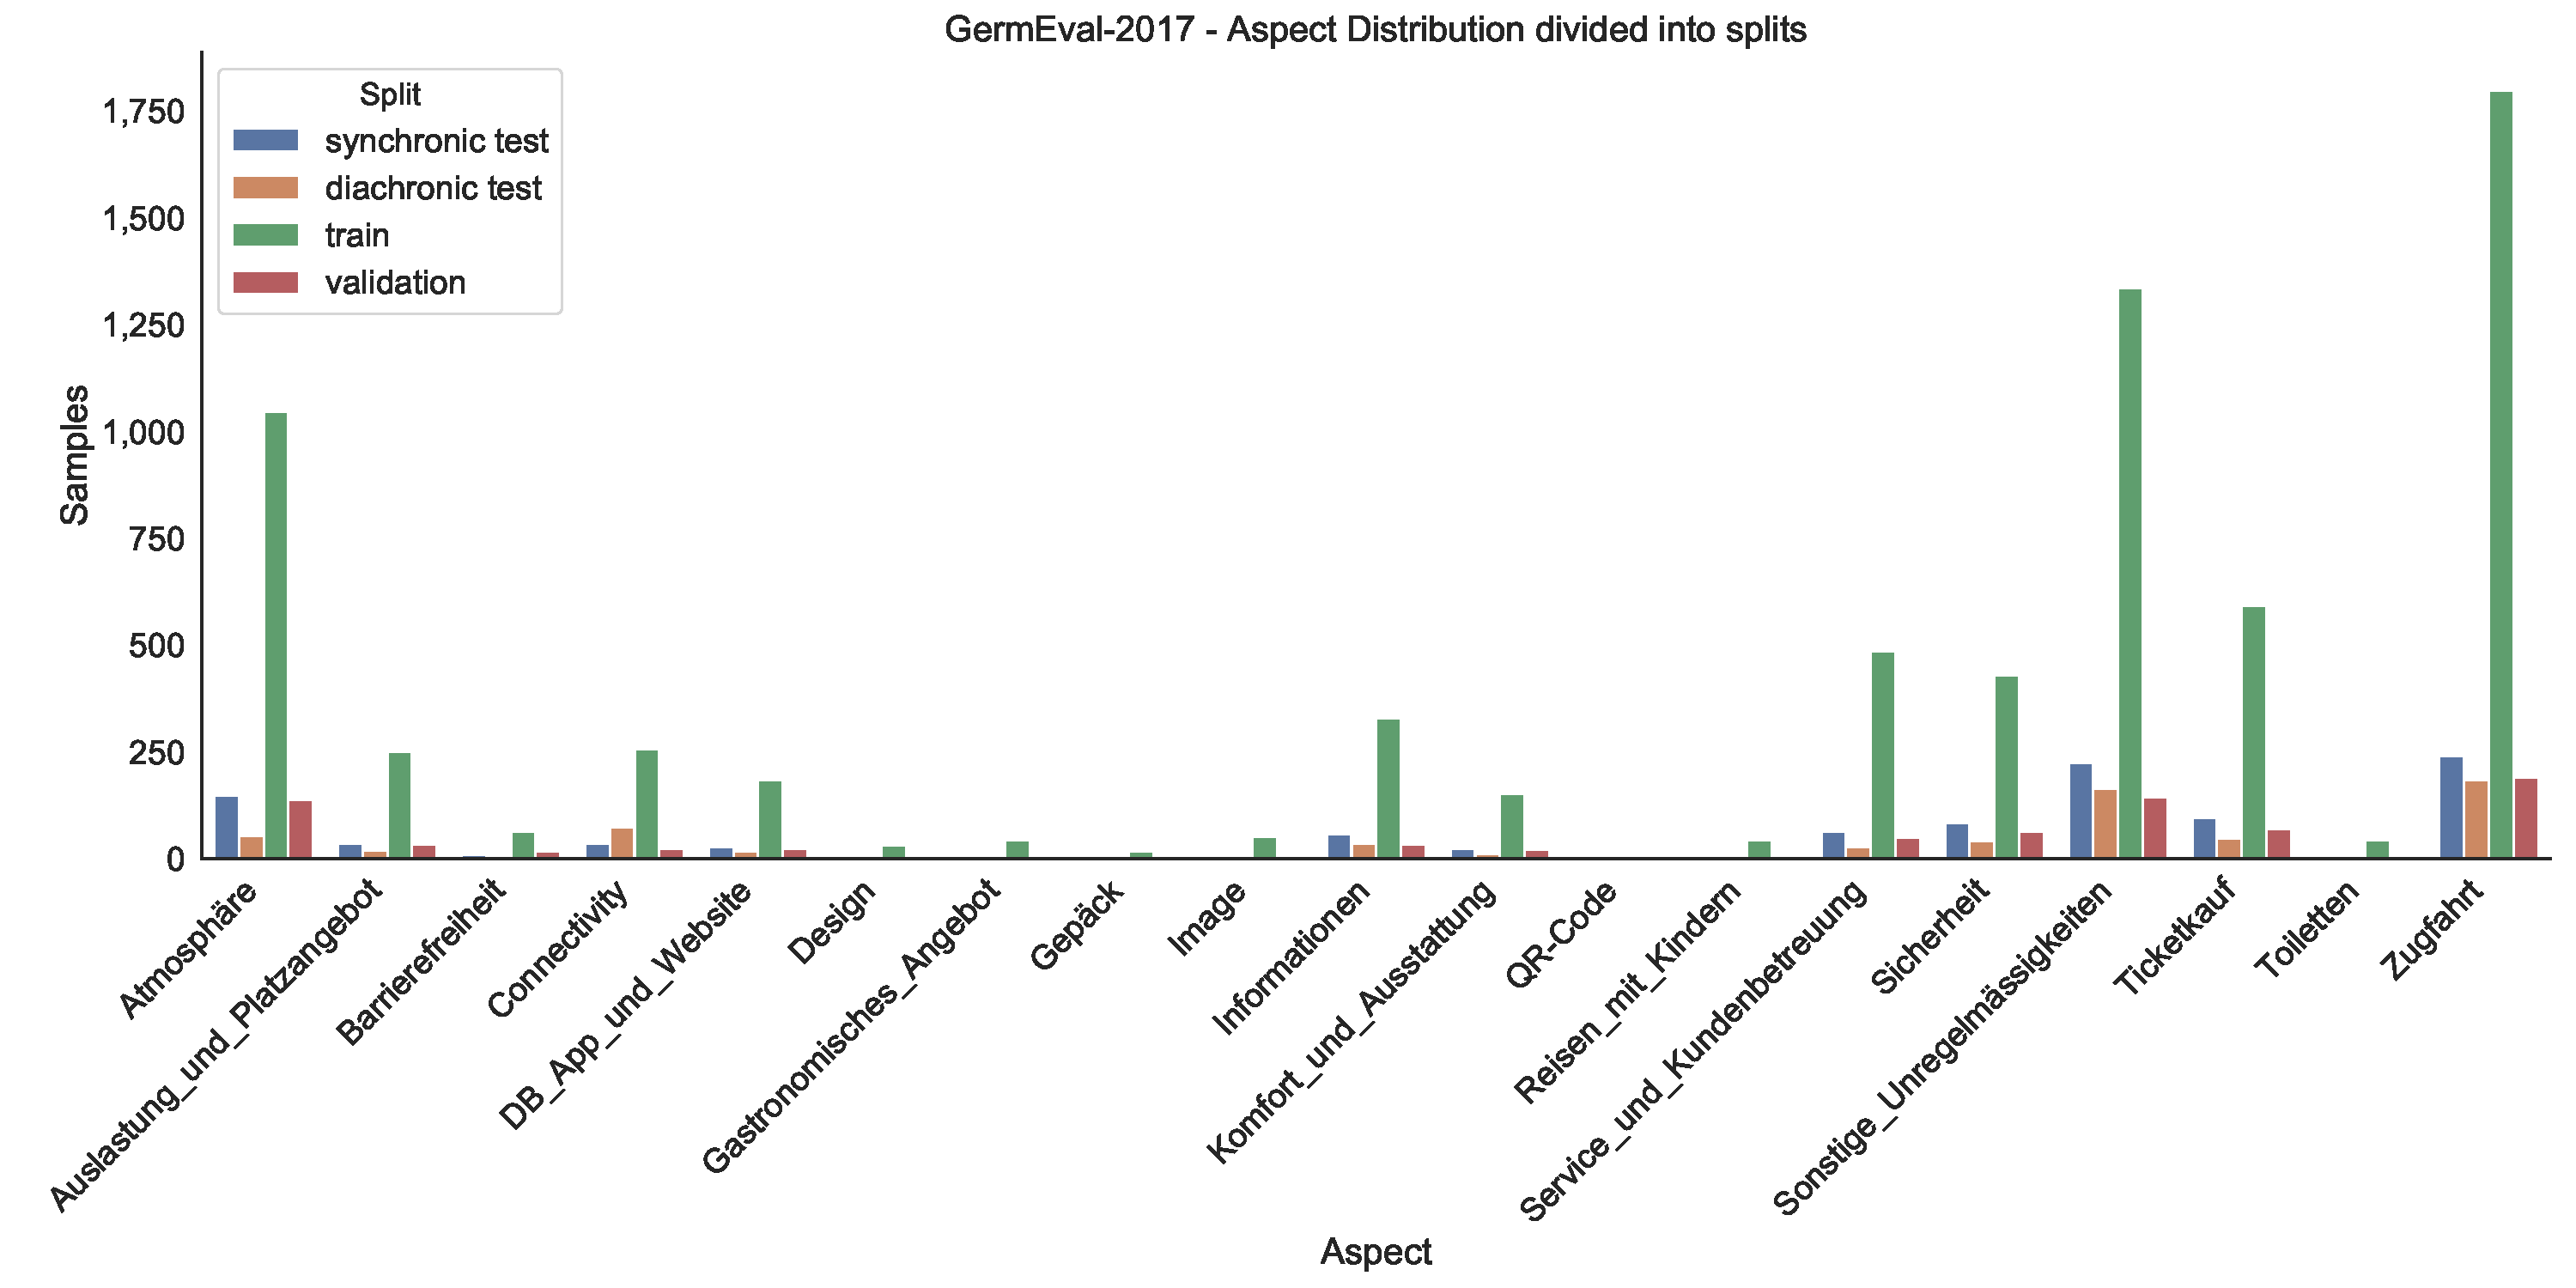
\includegraphics[width=\textwidth]{figures/08_appendix/08_germevalAspects}
    \caption{\textbf{GermEval-2017 -- Number of sentiment classes per aspect.} The graph shows how many samples are present for each aspect divided by data split.}
    \label{fig:08_germEvalStatistics}
\end{figure}

\subsection{Organic-2019 Data}

\subsubsection*{Entity -- Attribute Combinations}

\begin{multicols}{2}
    \begin{itemize}[leftmargin=*]
        \setlength\itemsep{-0.5em}

        \item[] GMOs:Nutritional quality, freshness 
        \item[] GMOs:chemicals pesticides 
        \item[] GMOs:environment
        \item[] GMOs:general
        \item[] GMOs:healthiness
        \item[] GMOs:label 
        \item[] GMOs:origin source 
        \item[] GMOs:price 
        \item[] GMOs:productivity 
        \item[] GMOs:safety
        \item[] GMOs:taste 
        \item[] convent. co.:animal welfare 
        \item[] convent. co.:availability
        \item[] convent. co.:chemicals pesticides
        \item[] convent. co.:environment 
        \item[] convent. co.:general 
        \item[] convent. co.:label
        \item[] convent. co.:productivity
        \item[] convent. co.:safety 
        \item[] convent. co.:taste
        \item[] convent. farming:Nutritional quality, freshness 
        \item[] convent. farming:animal welfare
        \item[] convent. farming:availability 
        \item[] convent. farming:chemicals pesticides 
        \item[] convent. farming:environment
        \item[] convent. farming:general
        \item[] convent. farming:healthiness
        \item[] convent. farming:label 
        \item[] convent. farming:origin source 
        \item[] convent. farming:price 
        \item[] convent. farming:productivity 
        \item[] convent. farming:safety
        \item[] convent. farming:taste 
        \item[] convent. general:Nutritional quality, freshness 
        \item[] convent. general:chemicals pesticides 
        \item[] convent. general:environment
        \item[] convent. general:general
        \item[] convent. general:healthiness
        \item[] convent. general:label 
        \item[] convent. general:origin source 
        \item[] convent. general:price 
        \item[] convent. general:productivity 
        \item[] convent. general:safety
        \item[] convent. products:Nutritional quality, freshness
        \item[] convent. products:animal welfare
        \item[] convent. products:availability 
        \item[] convent. products:chemicals pesticides 
        \item[] convent. products:environment 
        \item[] convent. products:general 
        \item[] convent. products:healthiness 
        \item[] convent. products:label
        \item[] convent. products:local
        \item[] convent. products:origin source
        \item[] convent. products:price
        \item[] convent. products:productivity 
        \item[] convent. products:safety
        \item[] convent. products:taste
        \item[] organic co.:Nutritional quality, freshness
        \item[] organic co.:animal welfare
        \item[] organic co.:availability 
        \item[] organic co.:chemicals pesticides 
        \item[] organic co.:environment 
        \item[] organic co.:general 
        \item[] organic co.:healthiness 
        \item[] organic co.:label
        \item[] organic co.:local
        \item[] organic co.:origin source
        \item[] organic co.:price
        \item[] organic co.:productivity 
        \item[] organic co.:safety
        \item[] organic co.:taste
        \item[] organic farmers:Nutritional quality, freshness 
        \item[] organic farmers:animal welfare 
        \item[] organic farmers:availability
        \item[] organic farmers:chemicals pesticides
        \item[] organic farmers:environment
        \item[] organic farmers:general
        \item[] organic farmers:healthiness
        \item[] organic farmers:label 
        \item[] organic farmers:local 
        \item[] organic farmers:origin source 
        \item[] organic farmers:price 
        \item[] organic farmers:productivity
        \item[] organic farmers:safety 
        \item[] organic farmers:taste 
        \item[] organic general:Nutritional quality, freshness 
        \item[] organic general:animal welfare 
        \item[] organic general:availability
        \item[] organic general:chemicals pesticides
        \item[] organic general:environment
        \item[] organic general:general
        \item[] organic general:healthiness
        \item[] organic general:label 
        \item[] organic general:local 
        \item[] organic general:origin source 
        \item[] organic general:price 
        \item[] organic general:productivity
        \item[] organic general:safety 
        \item[] organic general:taste 
        \item[] organic products:Nutritional quality, freshness 
        \item[] organic products:animal welfare
        \item[] organic products:availability 
        \item[] organic products:chemicals pesticides 
        \item[] organic products:environment
        \item[] organic products:general
        \item[] organic products:healthiness
        \item[] organic products:label 
        \item[] organic products:local 
        \item[] organic products:origin source 
        \item[] organic products:price 
        \item[] organic products:productivity 
        \item[] organic products:safety
        \item[] organic products:taste 
        \label{li:08_og_aspects} 
    \end{itemize}
\end{multicols}

\subsubsection*{Coarse Partition -- Combinations}

\begin{multicols}{2}
    \begin{itemize}[leftmargin=*]
        \setlength\itemsep{-0.5em}
        \item[] GMO:environment 
        \item[] GMO:experienced quality 
        \item[] GMO:general 
        \item[] GMO:price
        \item[] GMO:safety and healthiness
        \item[] GMO:trustworthy sources 
        \item[] conventional:environment 
        \item[] conventional:experienced quality 
        \item[] conventional:general 
        \item[] conventional:price
        \item[] conventional:safety and healthiness 
        \item[] conventional:trustworthy sources 
        \item[] organic:environment 
        \item[] organic:experienced quality 
        \item[] organic:general 
        \item[] organic:price
        \item[] organic:safety and healthiness
        \item[] organic:trustworthy sources
        \label{li:08_og_aspectsCoarse}  
    \end{itemize}
\end{multicols}

\subsubsection*{Distribution of Entities and Attributes}

\begin{figure}[H]
    \centering
    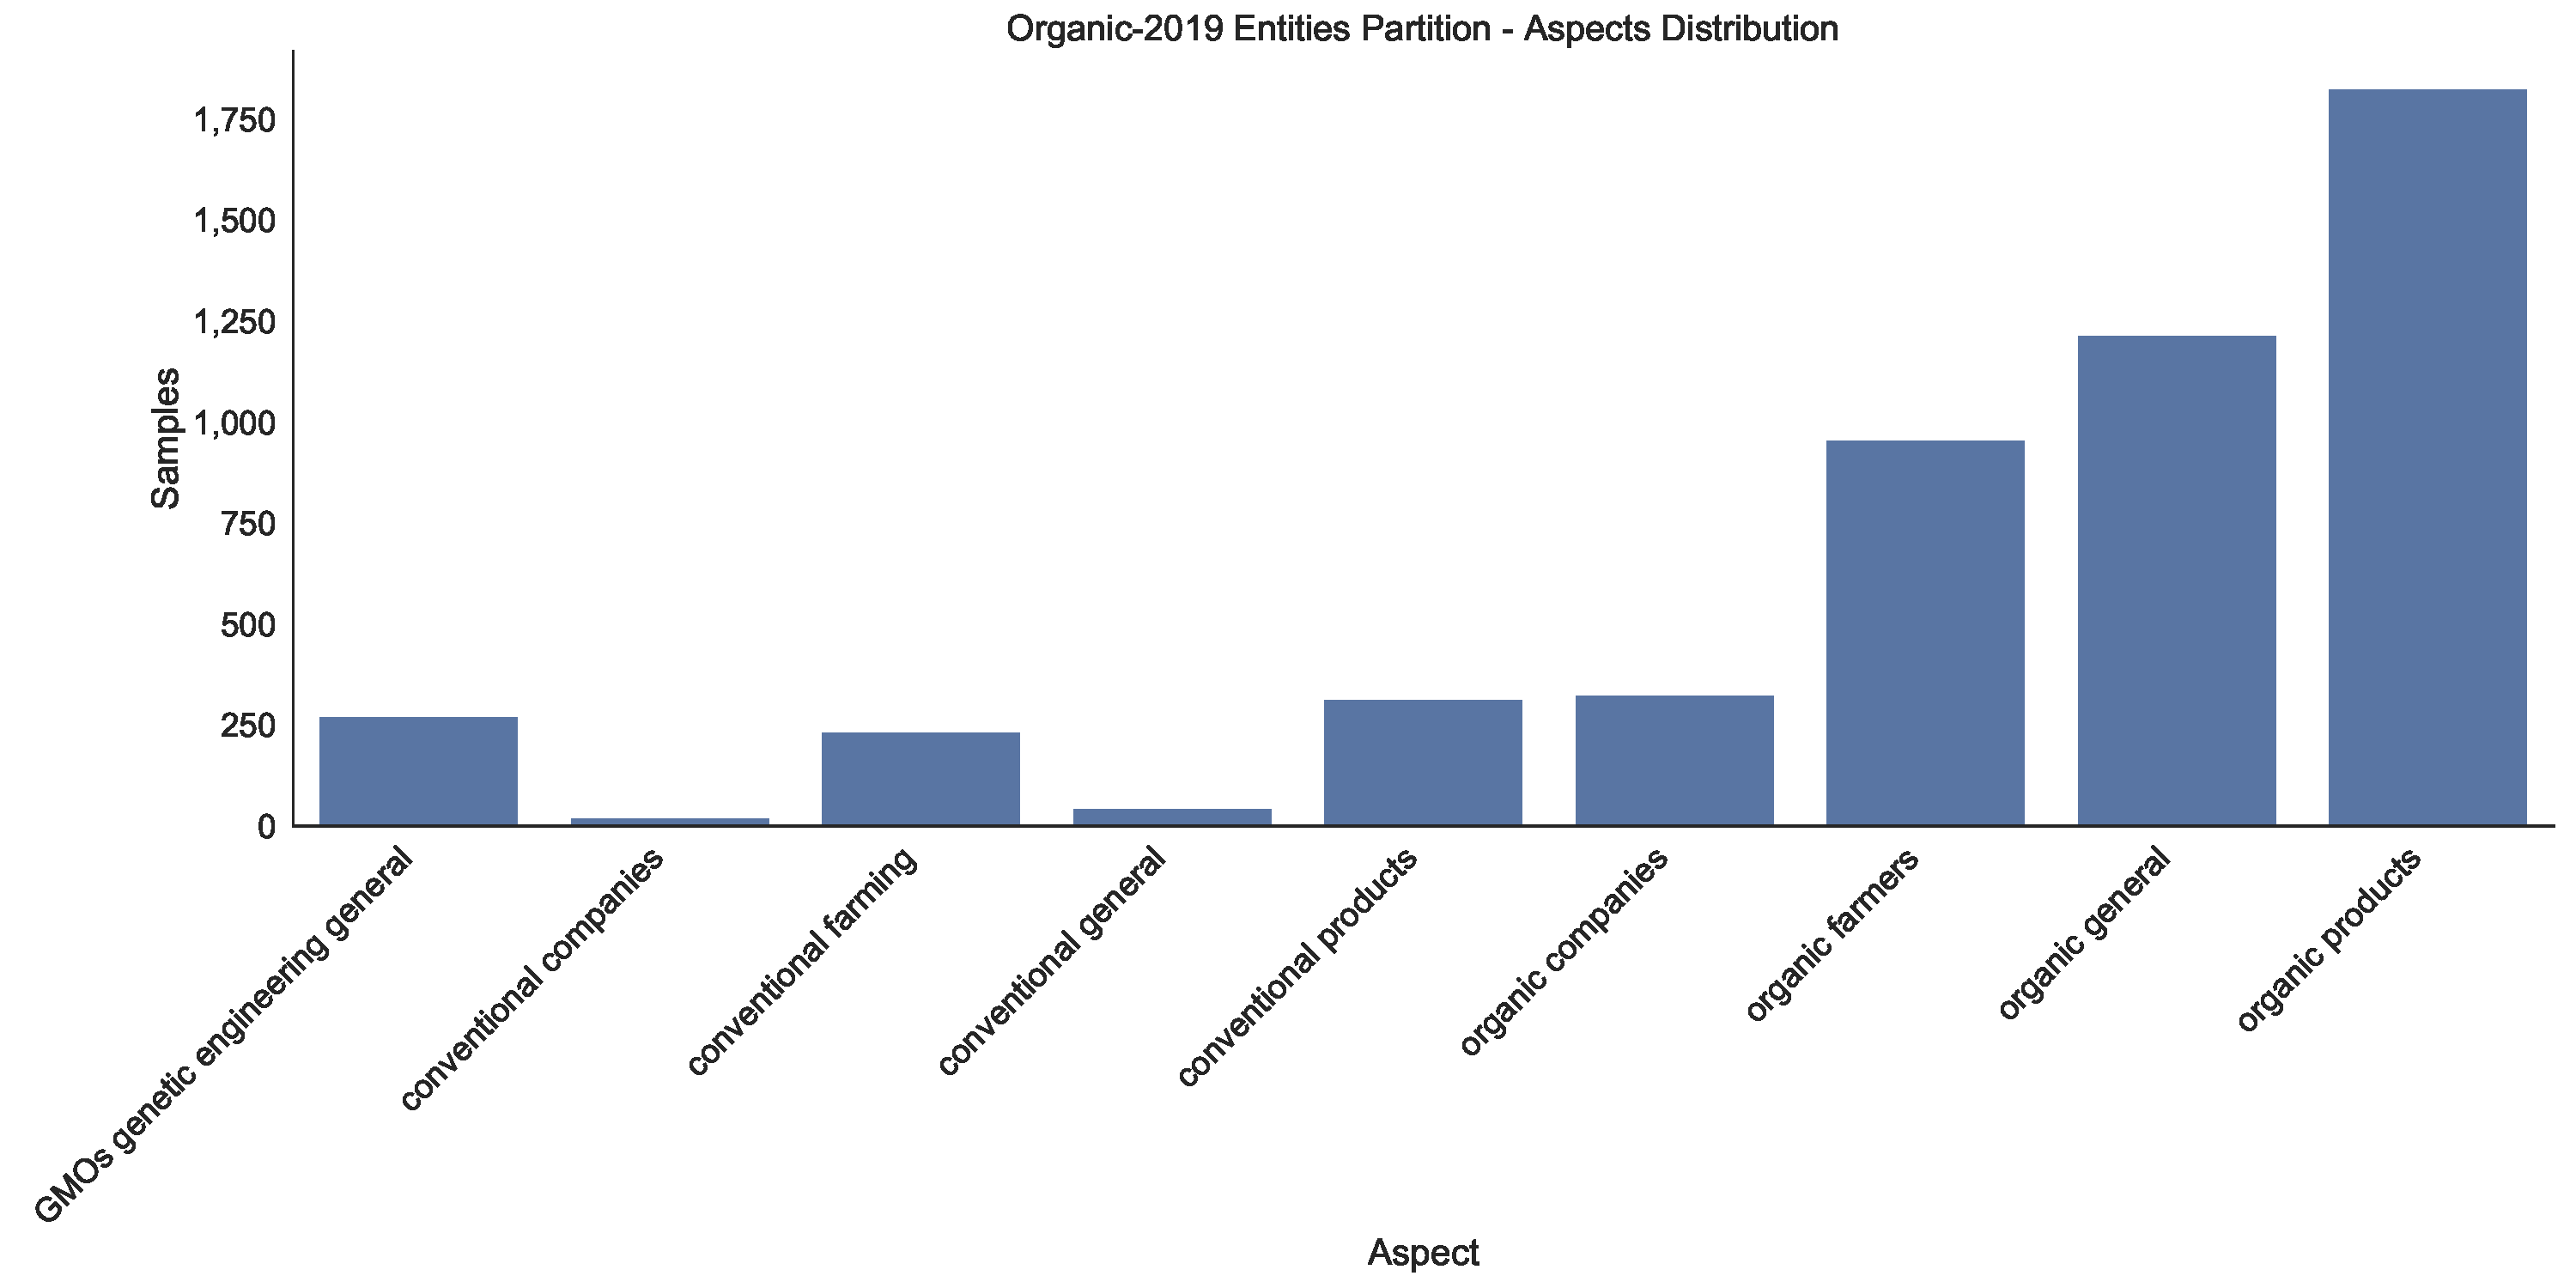
\includegraphics[width=\textwidth]{figures/05_setup/05_organicEntities}
    \caption{\textbf{Organic-2019 -- Entities} Distribution of the aspect \textit{entity} in the Organic-2019 dataset.}
    \label{fig:05_organic2019_Entities}
\end{figure}

\begin{figure}[H]
    \centering
    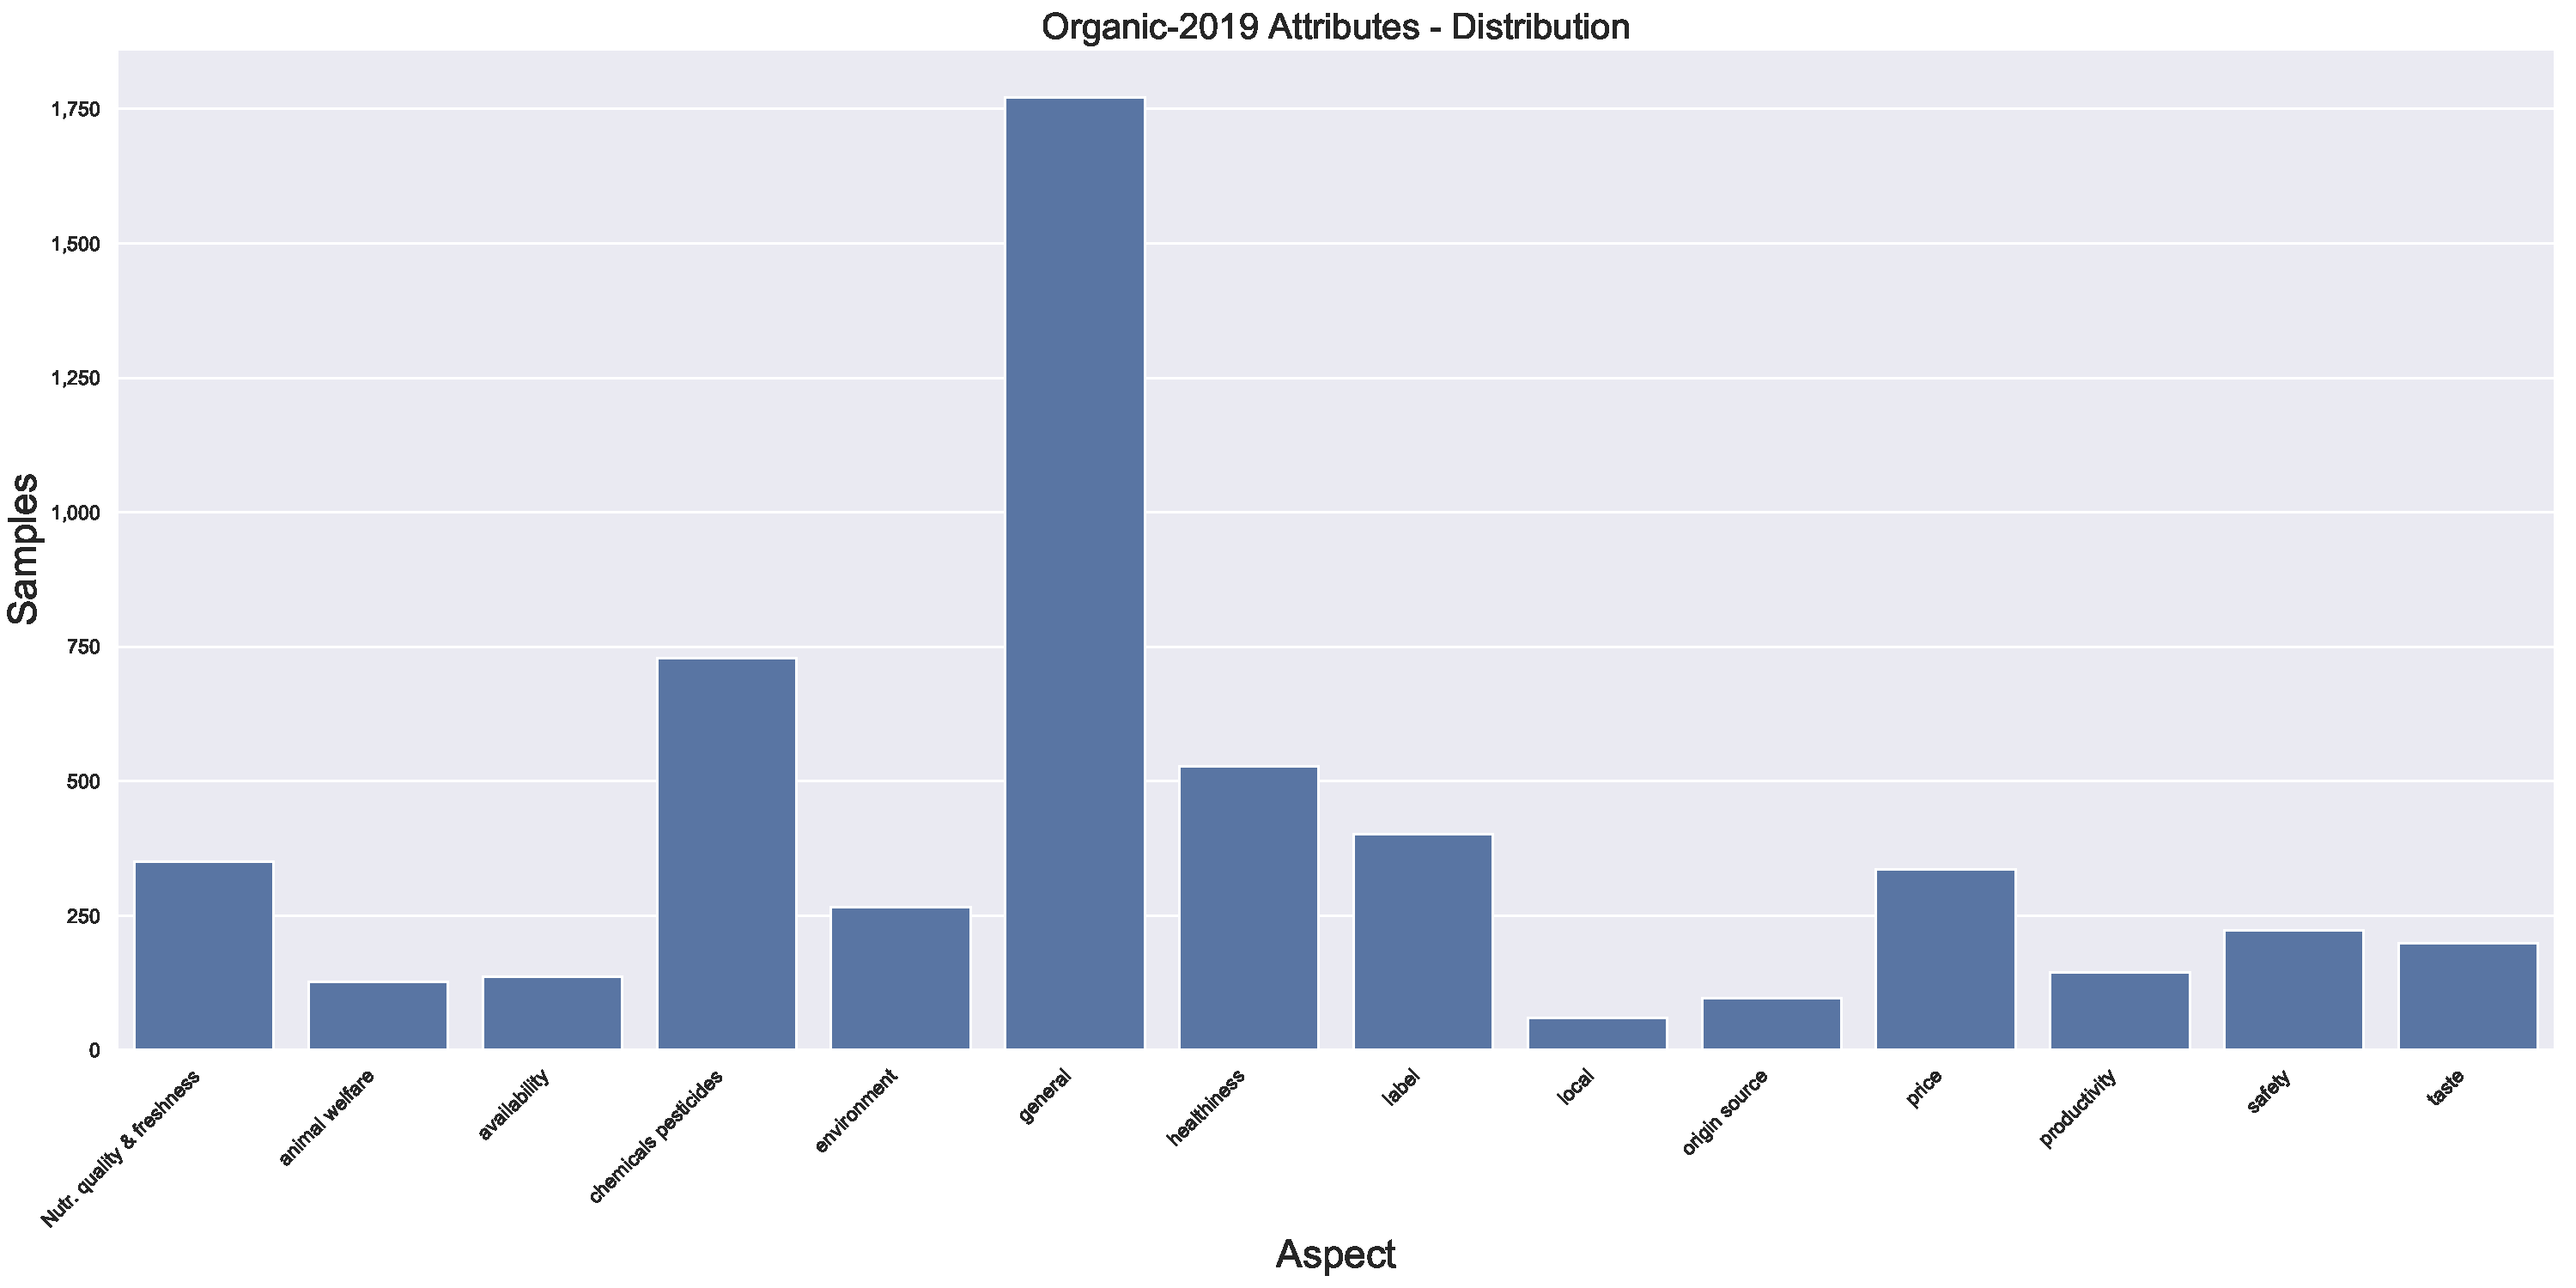
\includegraphics[width=\textwidth]{figures/05_setup/05_organicAttributes}
    \caption{\textbf{Organic-2019 -- Attributes} Distribution of the aspect \textit{attribute} in the Organic-2019 dataset.}
    \label{fig:05_organic2019_Attributes}
\end{figure}

    

\section{Optimization}

\begin{table}[H]
    \begin{center}
        \begin{tabular}{lclc}
        \toprule
        \multicolumn{4}{c}{OLS regression for Validation Loss / HyperOpt Iterations} \\
        \midrule
        \textbf{Dep. Variable:}    &        y        & \textbf{  R-squared:        } &     0.009   \\
        \textbf{Model:}            &       OLS       & \textbf{  Adj. R-squared:   } &    -0.002   \\
        \textbf{Method:}           &  Least Squares  & \textbf{  F-statistic:      } &    0.8307   \\
        \textbf{Date:}             & Mi, 24 Apr 2019 & \textbf{  Prob (F-statistic):} &    0.365    \\
        \textbf{Time:}             &     15:32:34    & \textbf{  Log-Likelihood:   } &   -51.223   \\
        \textbf{No. Observations:} &          90     & \textbf{  AIC:              } &     106.4   \\
        \textbf{Df Residuals:}     &          88     & \textbf{  BIC:              } &     111.4   \\
        \textbf{Df Model:}         &           1     & \textbf{                     } &             \\
        \bottomrule
        \end{tabular}
        \begin{tabular}{lcccccc}
                       & \textbf{coef} & \textbf{std err} & \textbf{t} & \textbf{P$>$$|$t$|$} & \textbf{[0.025} & \textbf{0.975]}  \\
        \midrule
        \textbf{const} &       0.3598  &        0.090     &     3.980  &         0.000        &        0.180    &        0.539     \\
        \textbf{x1}    &      -0.0016  &        0.002     &    -0.911  &         0.365        &       -0.005    &        0.002     \\
        \bottomrule
        \end{tabular}
        \begin{tabular}{lclc}
        \textbf{Omnibus:}       & 163.475 & \textbf{  Durbin-Watson:    } &     2.062  \\
        \textbf{Prob(Omnibus):} &   0.000 & \textbf{  Jarque-Bera (JB): } & 11634.826  \\
        \textbf{Skew:}          &   6.940 & \textbf{  Prob(JB):         } &      0.00  \\
        \textbf{Kurtosis:}      &  56.944 & \textbf{  Cond. No.          } &      102.  \\
        \bottomrule
        \end{tabular}
    \end{center}
    \caption{\textbf{\gls{ols} Regression statistics} for a regression of HyperOpt \gls{tpe} optimization losses on the validation set {(Dataset:GermEval-2017)}}
    \label{tab:08_olsLossItVal}    
\end{table}

\begin{table}[H]
    \begin{center}
        \begin{tabular}{lclc}
        \toprule
        \multicolumn{4}{c}{OLS regression for Test Loss / HyperOpt Iterations} \\
        \midrule
        \textbf{Dep. Variable:}    &        y        & \textbf{  R-squared:        } &     0.006   \\
        \textbf{Model:}            &       OLS       & \textbf{  Adj. R-squared:   } &    -0.006   \\
        \textbf{Method:}           &  Least Squares  & \textbf{  F-statistic:      } &    0.4930   \\
        \textbf{Date:}             & Mi, 24 Apr 2019 & \textbf{  Prob (F-statistic):} &    0.484    \\
        \textbf{Time:}             &     16:22:21    & \textbf{  Log-Likelihood:   } &   -206.16   \\
        \textbf{No. Observations:} &          90     & \textbf{  AIC:              } &     416.3   \\
        \textbf{Df Residuals:}     &          88     & \textbf{  BIC:              } &     421.3   \\
        \textbf{Df Model:}         &           1     & \textbf{                     } &             \\
        \bottomrule
        \end{tabular}
        \begin{tabular}{lcccccc}
                    & \textbf{coef} & \textbf{std err} & \textbf{t} & \textbf{P$>$$|$t$|$} & \textbf{[0.025} & \textbf{0.975]}  \\
        \midrule
        \textbf{const} &       0.8356  &        0.506     &     1.653  &         0.102        &       -0.169    &        1.840     \\
        \textbf{x1}    &      -0.0069  &        0.010     &    -0.702  &         0.484        &       -0.026    &        0.013     \\
        \bottomrule
        \end{tabular}
        \begin{tabular}{lclc}
        \textbf{Omnibus:}       & 191.171 & \textbf{  Durbin-Watson:    } &     2.030  \\
        \textbf{Prob(Omnibus):} &   0.000 & \textbf{  Jarque-Bera (JB): } & 25929.119  \\
        \textbf{Skew:}          &   9.027 & \textbf{  Prob(JB):         } &      0.00  \\
        \textbf{Kurtosis:}      &  84.169 & \textbf{  Cond. No.          } &      102.  \\
        \bottomrule
        \end{tabular}
    \end{center}
    \caption{\textbf{\gls{ols} Regression statistics} for a regression of HyperOpt \gls{tpe} optimization losses on the test set {(Dataset:GermEval-2017)}}
    \label{tab:08_olsLossItTest}    
\end{table}

\begin{table}[H]
    \centering
    \begin{tabular}{@{}lll@{}}
    \toprule
    Variable           & Type       & Parameters                \\ \midrule
    Batch Size         & QUniform   & Interval:{[}1, 100{]}    \\
    Comment Clipping   & QUniform   & Interval:{[}10, 250{]}   \\
    Replace URL Tokens & Bool       & {[}True, False{]}         \\
    Use Stop Words     & Bool       & {[}True, False{]}         \\
    Use Spell Checker  & Bool       & {[}True, False{]}         \\
    Harmonize Bahn     & Bool       & {[}True, False{]}         \\
    Embedding Type     & Choice     & {[}Glove, fastText{]}     \\
    \# Encoder Blocks  & QUniform   & Interval {[}1, 8{]}       \\
    \# Attention Heads & Choice     & {[}1, 2, 3, 4, 5{]}       \\
    PW Layer Size      & QUniform   & Interval:{[}32, 256{]}   \\
    TF Dropout         & Uniform    & Interval {[}0, 0.8{]}     \\
    Output Dropout     & Uniform    & Interval {[}0, 0.8{]}     \\
    Transformer Bias   & Bool       & {[}True, False{]}         \\
    LR Warmup          & QUniform   & Interval {[}1000, 9000{]} \\
    LR Factor          & Uniform    & Interval {[}0.01, 4{]}    \\
    Adam $\beta 1$        & Uniform    & Interval {[}0.7, 0.999{]} \\
    Adam $\beta 2$        & Uniform    & Interval {[}0.7, 0.999{]} \\
    Adam EPS           & LogUniform & log(1e-10), log(1)        \\
    LR                 & LogNormal  & log(0.01, log(10)         \\
    Weight Decay       & QUniform   & $1e^{[-8, -3]}$       \\
    Output Layer       & Choice     & {[}CNN*, LinSum{]}        \\
    \# CNN Filter*     & QUniform   & Interval {[}1, 400{]}     \\
    Kernel Size*       & QUniform   & Interval {[}1, 10{]}      \\
    Stride*            & QUniform   & Interval {[}1, 10{]}      \\
    Padding*           & QUniform   & Interval {[}0, 5{]}       \\ \bottomrule
    \end{tabular}
    \caption{\textbf{Hyperparameter Search space for GermEval-2017.} * marks parameters which are only sampled if CNN is chosen as the output layer.}
    \label{tab:08_hpSpace}    
\end{table}

\begin{figure}[H]
    \centering
    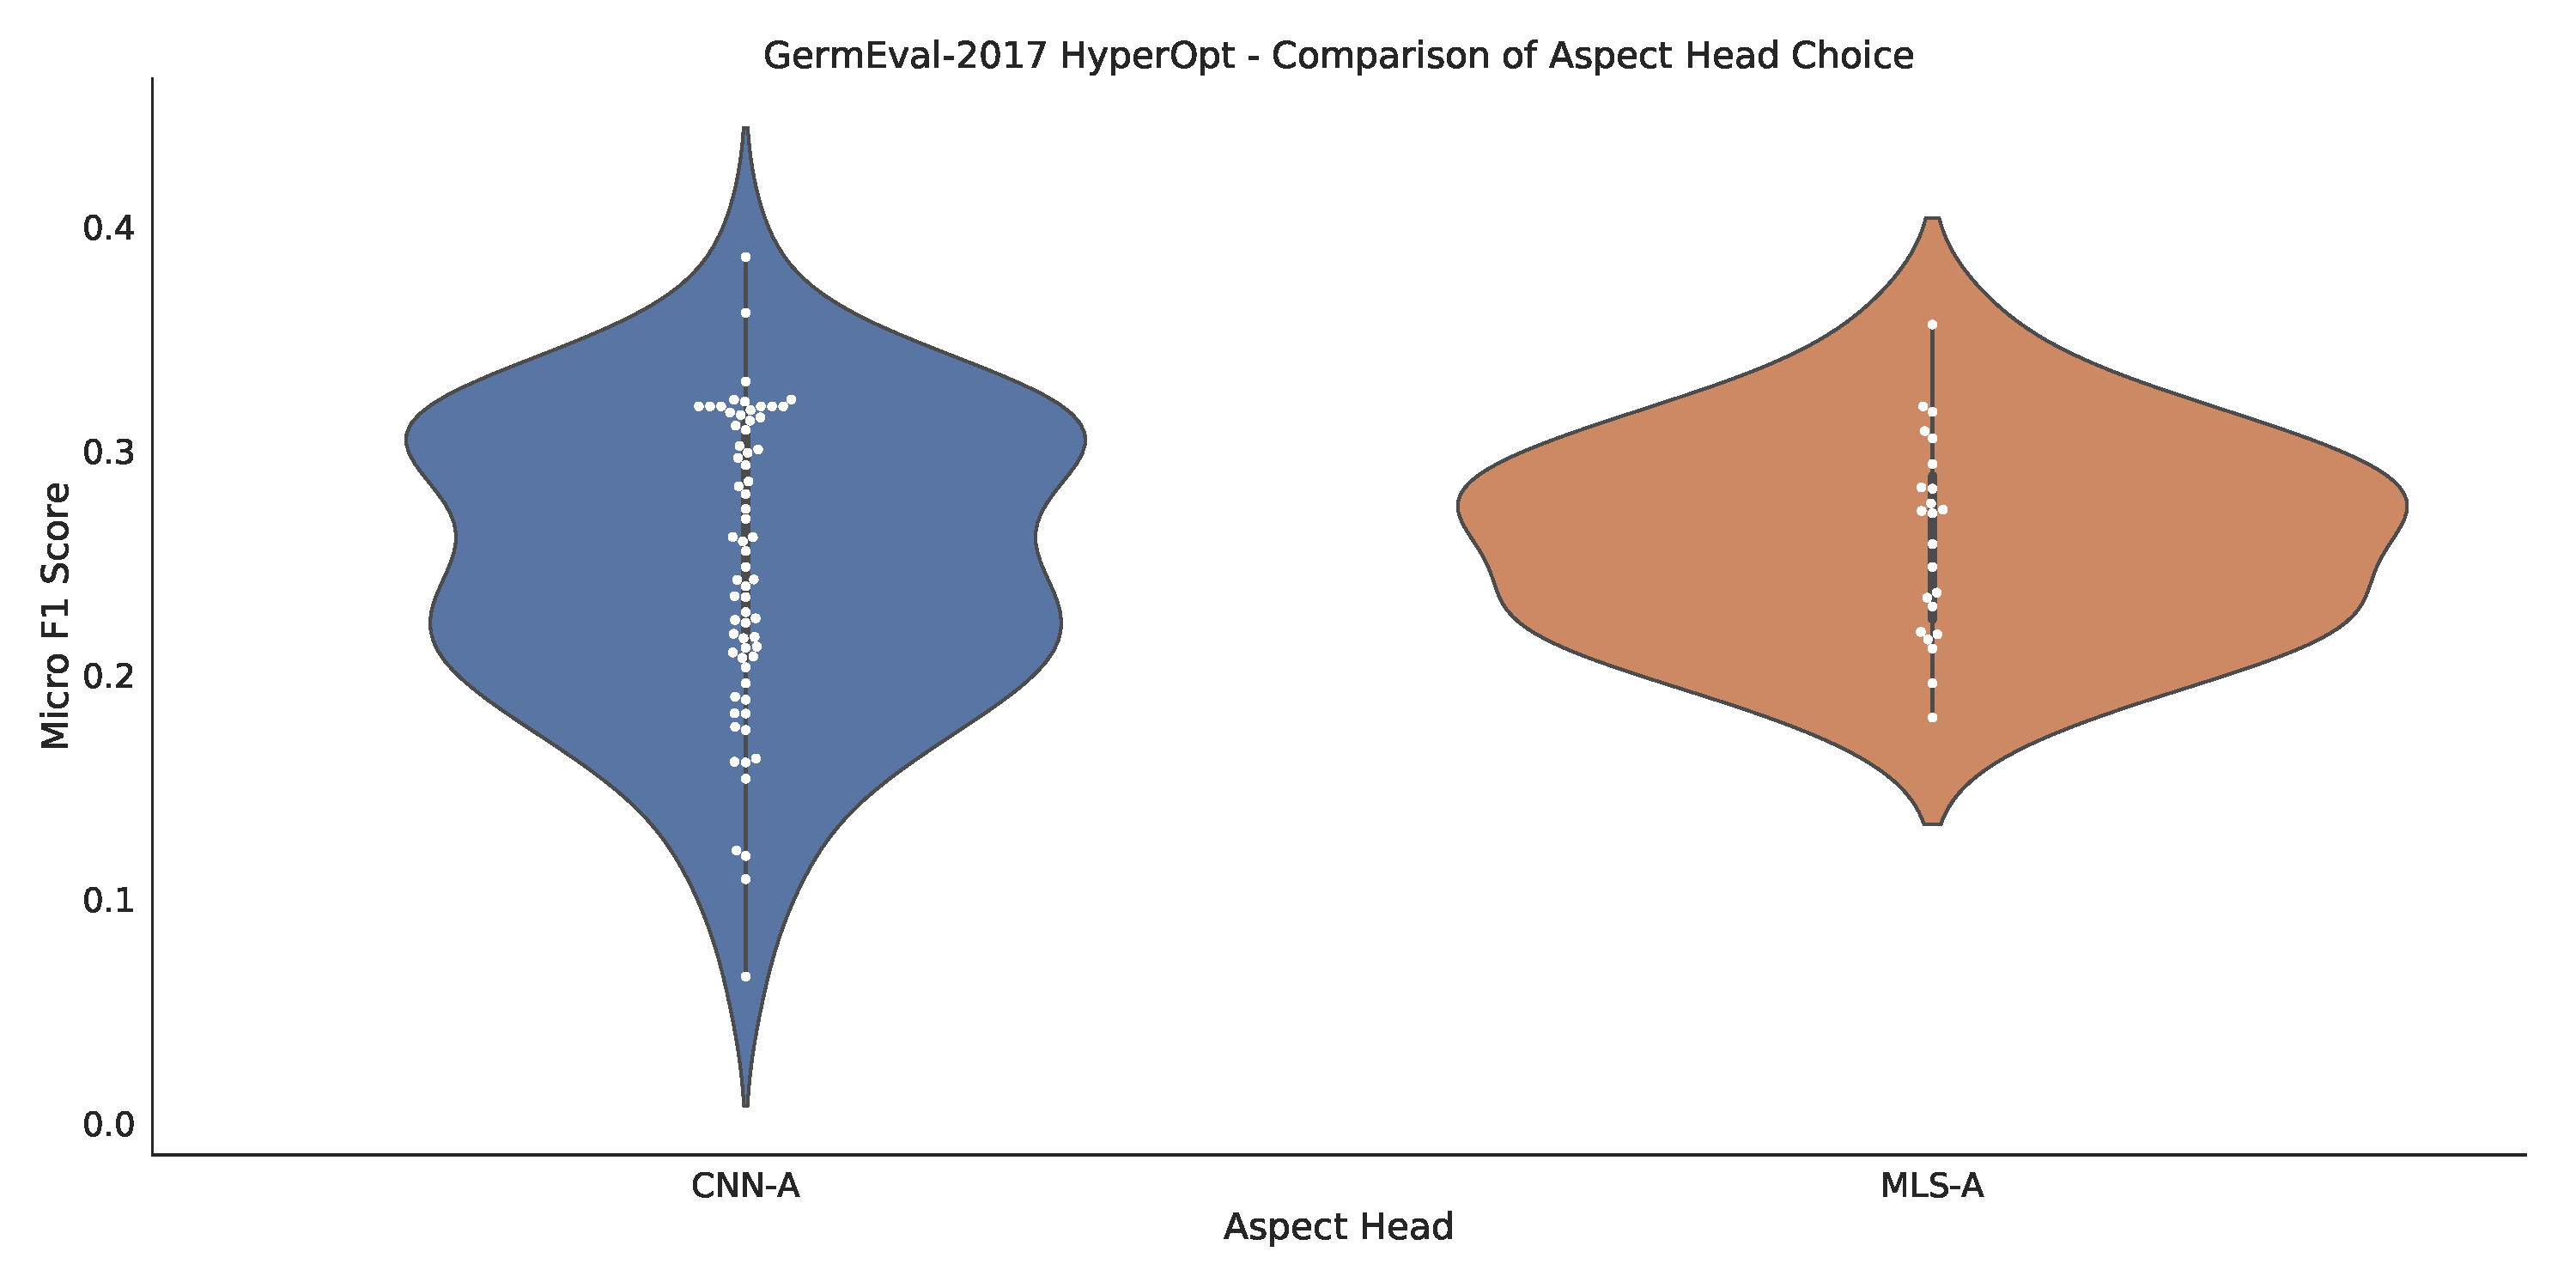
\includegraphics[width=\textwidth]{figures/06_results/06_hp_ge_vio_aspectHead_test}
    \caption{\textbf{Hyperopt -- Comparison and impact of aspect head choices and sampling amount}.}
    \label{fig:06_ge_aspectHeadChoices}
\end{figure}

\begin{figure}[H]
    \centering
    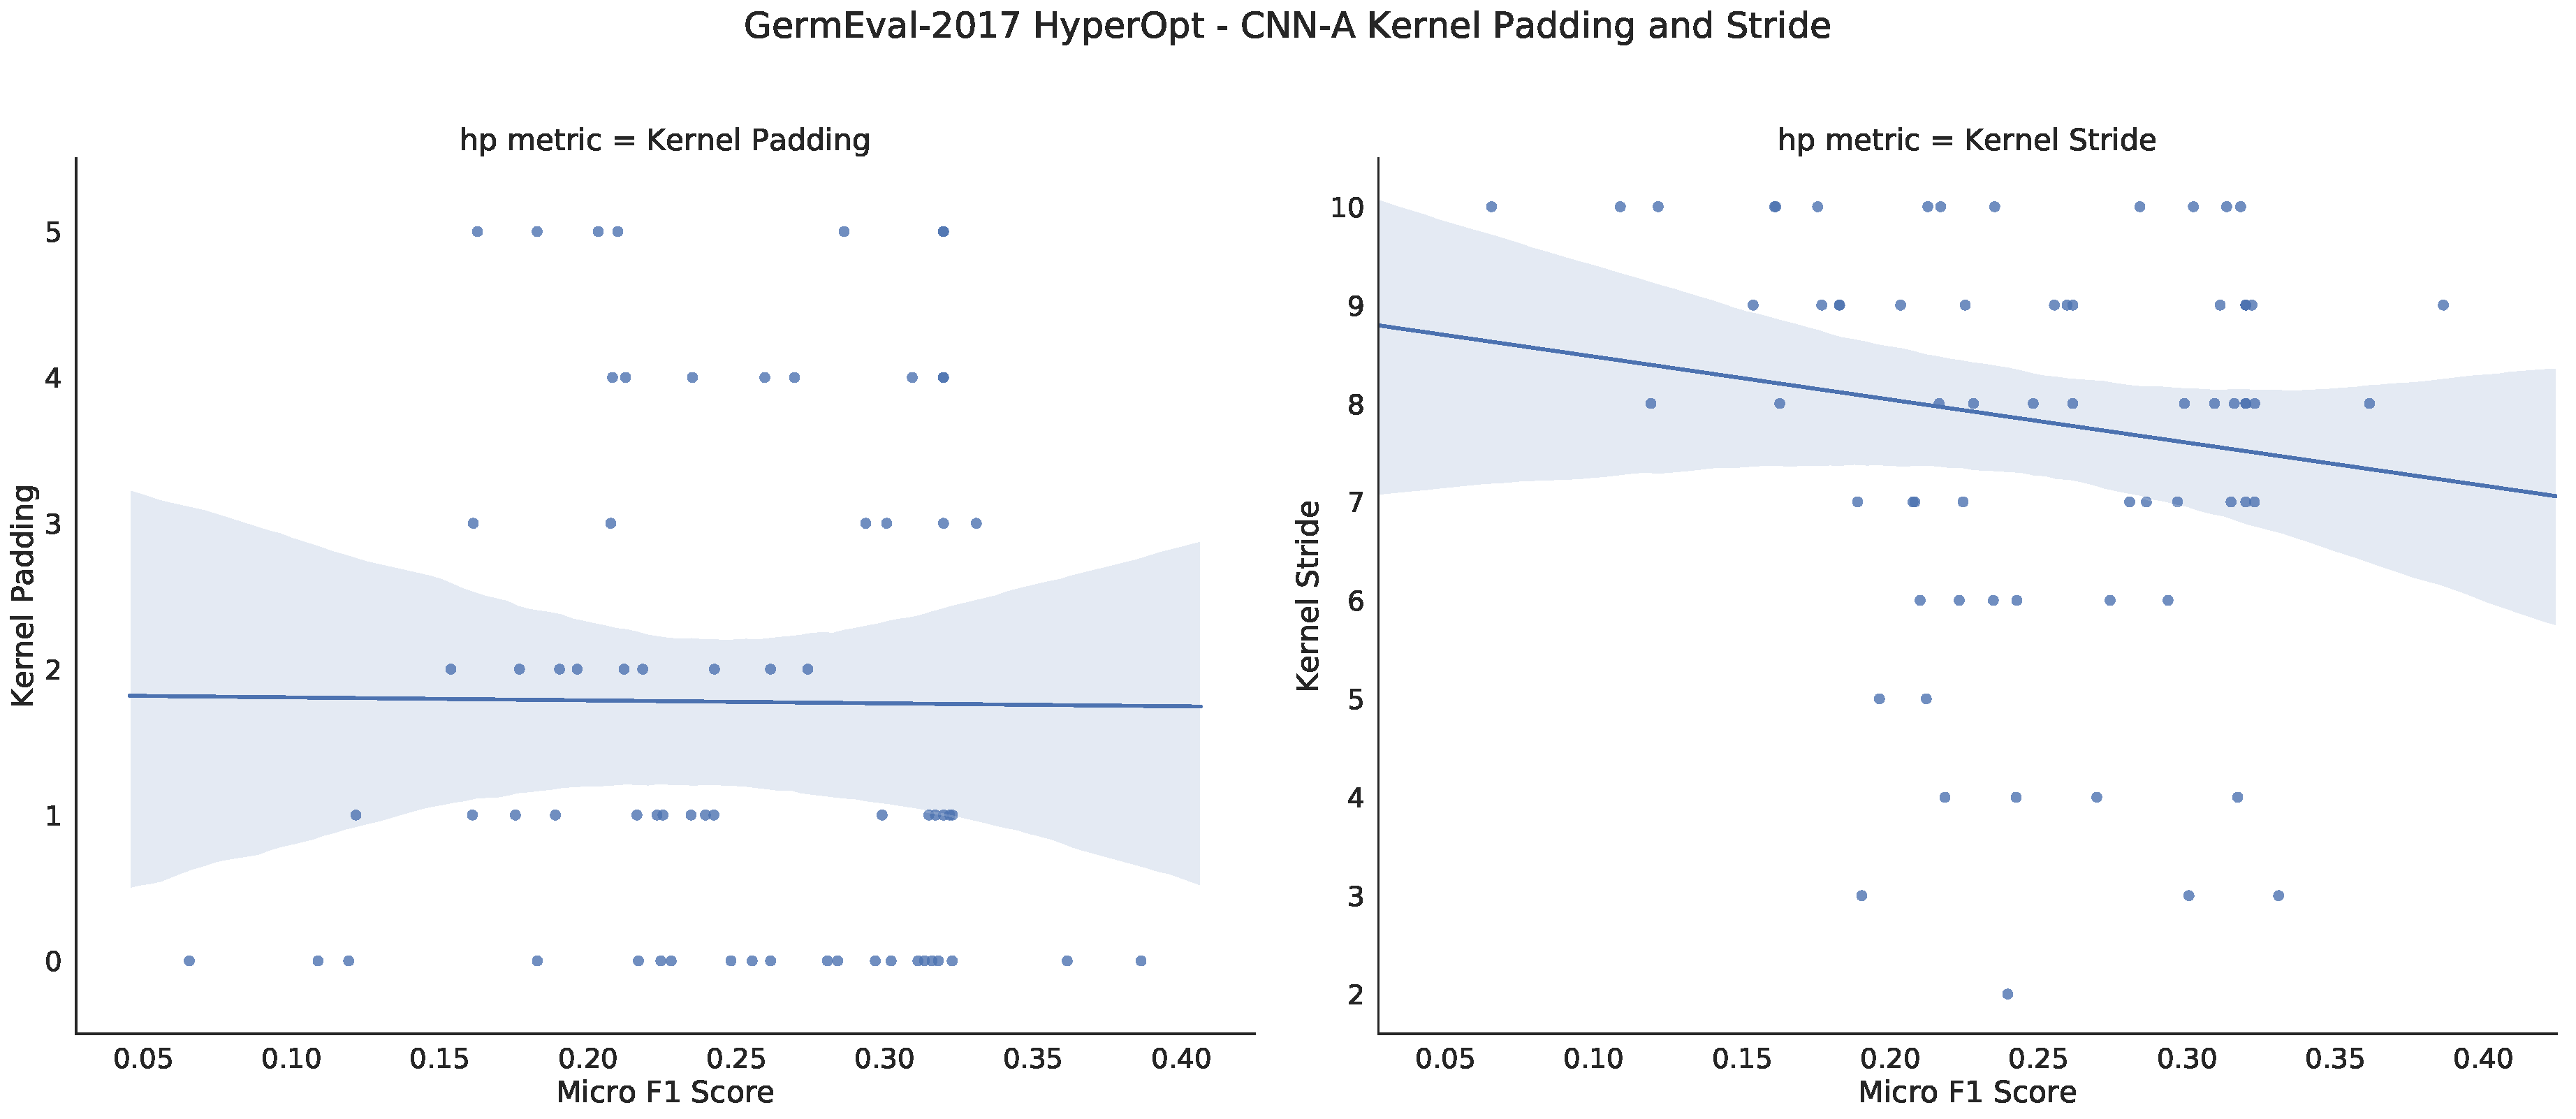
\includegraphics[width=\textwidth]{figures/06_results/06_hp_ge_lm_cnnParams2_test}
    \caption{\textbf{Impact of CNN parameters on micro F1-score.} The graph on the left shows the impact of the kernel padding on the model performance. The graph on the right depicts the influence of the kernel stride on the F1-score.}
    \label{fig:06_HpOptim_CnnParams2}
\end{figure}

\section{Results}

\subsection{GermEval-2017}

\begin{figure}[H]
    \centering

    \subfloat[Allgemein]{
        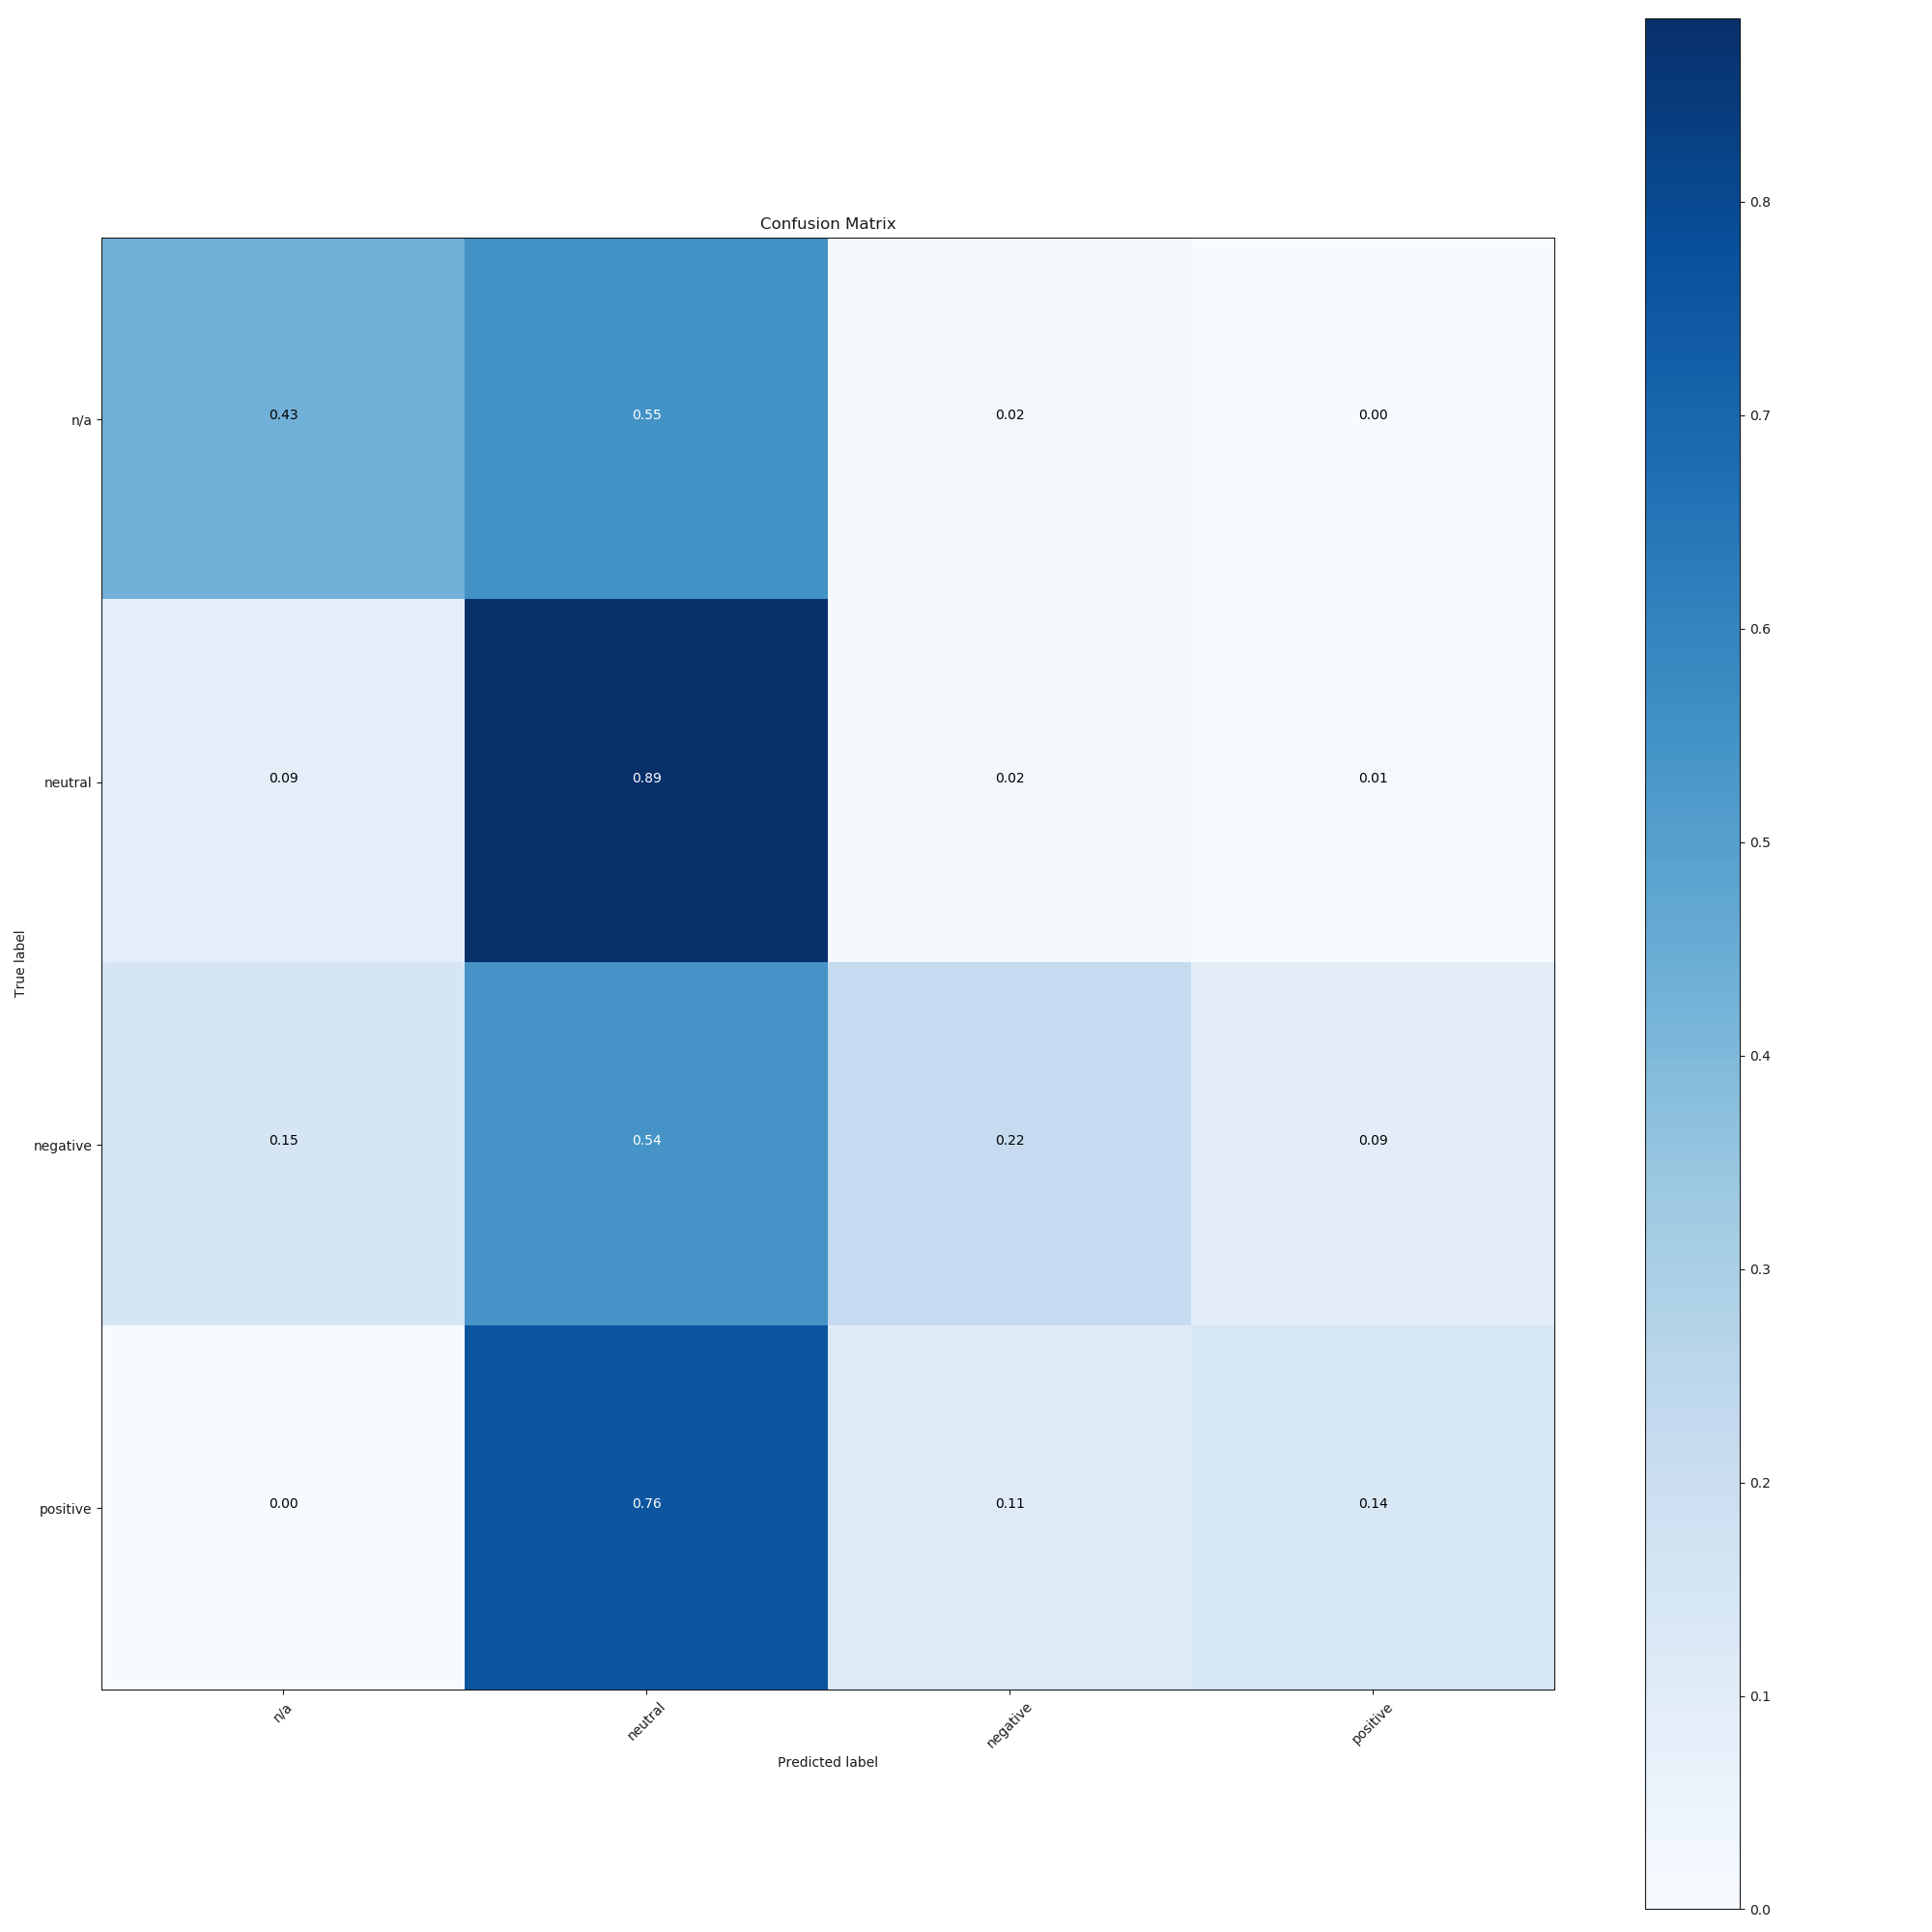
\includegraphics[width=0.19\textwidth]{figures/08_appendix/germeval/08_1}
    }
    \subfloat[Atmosphäre]{
        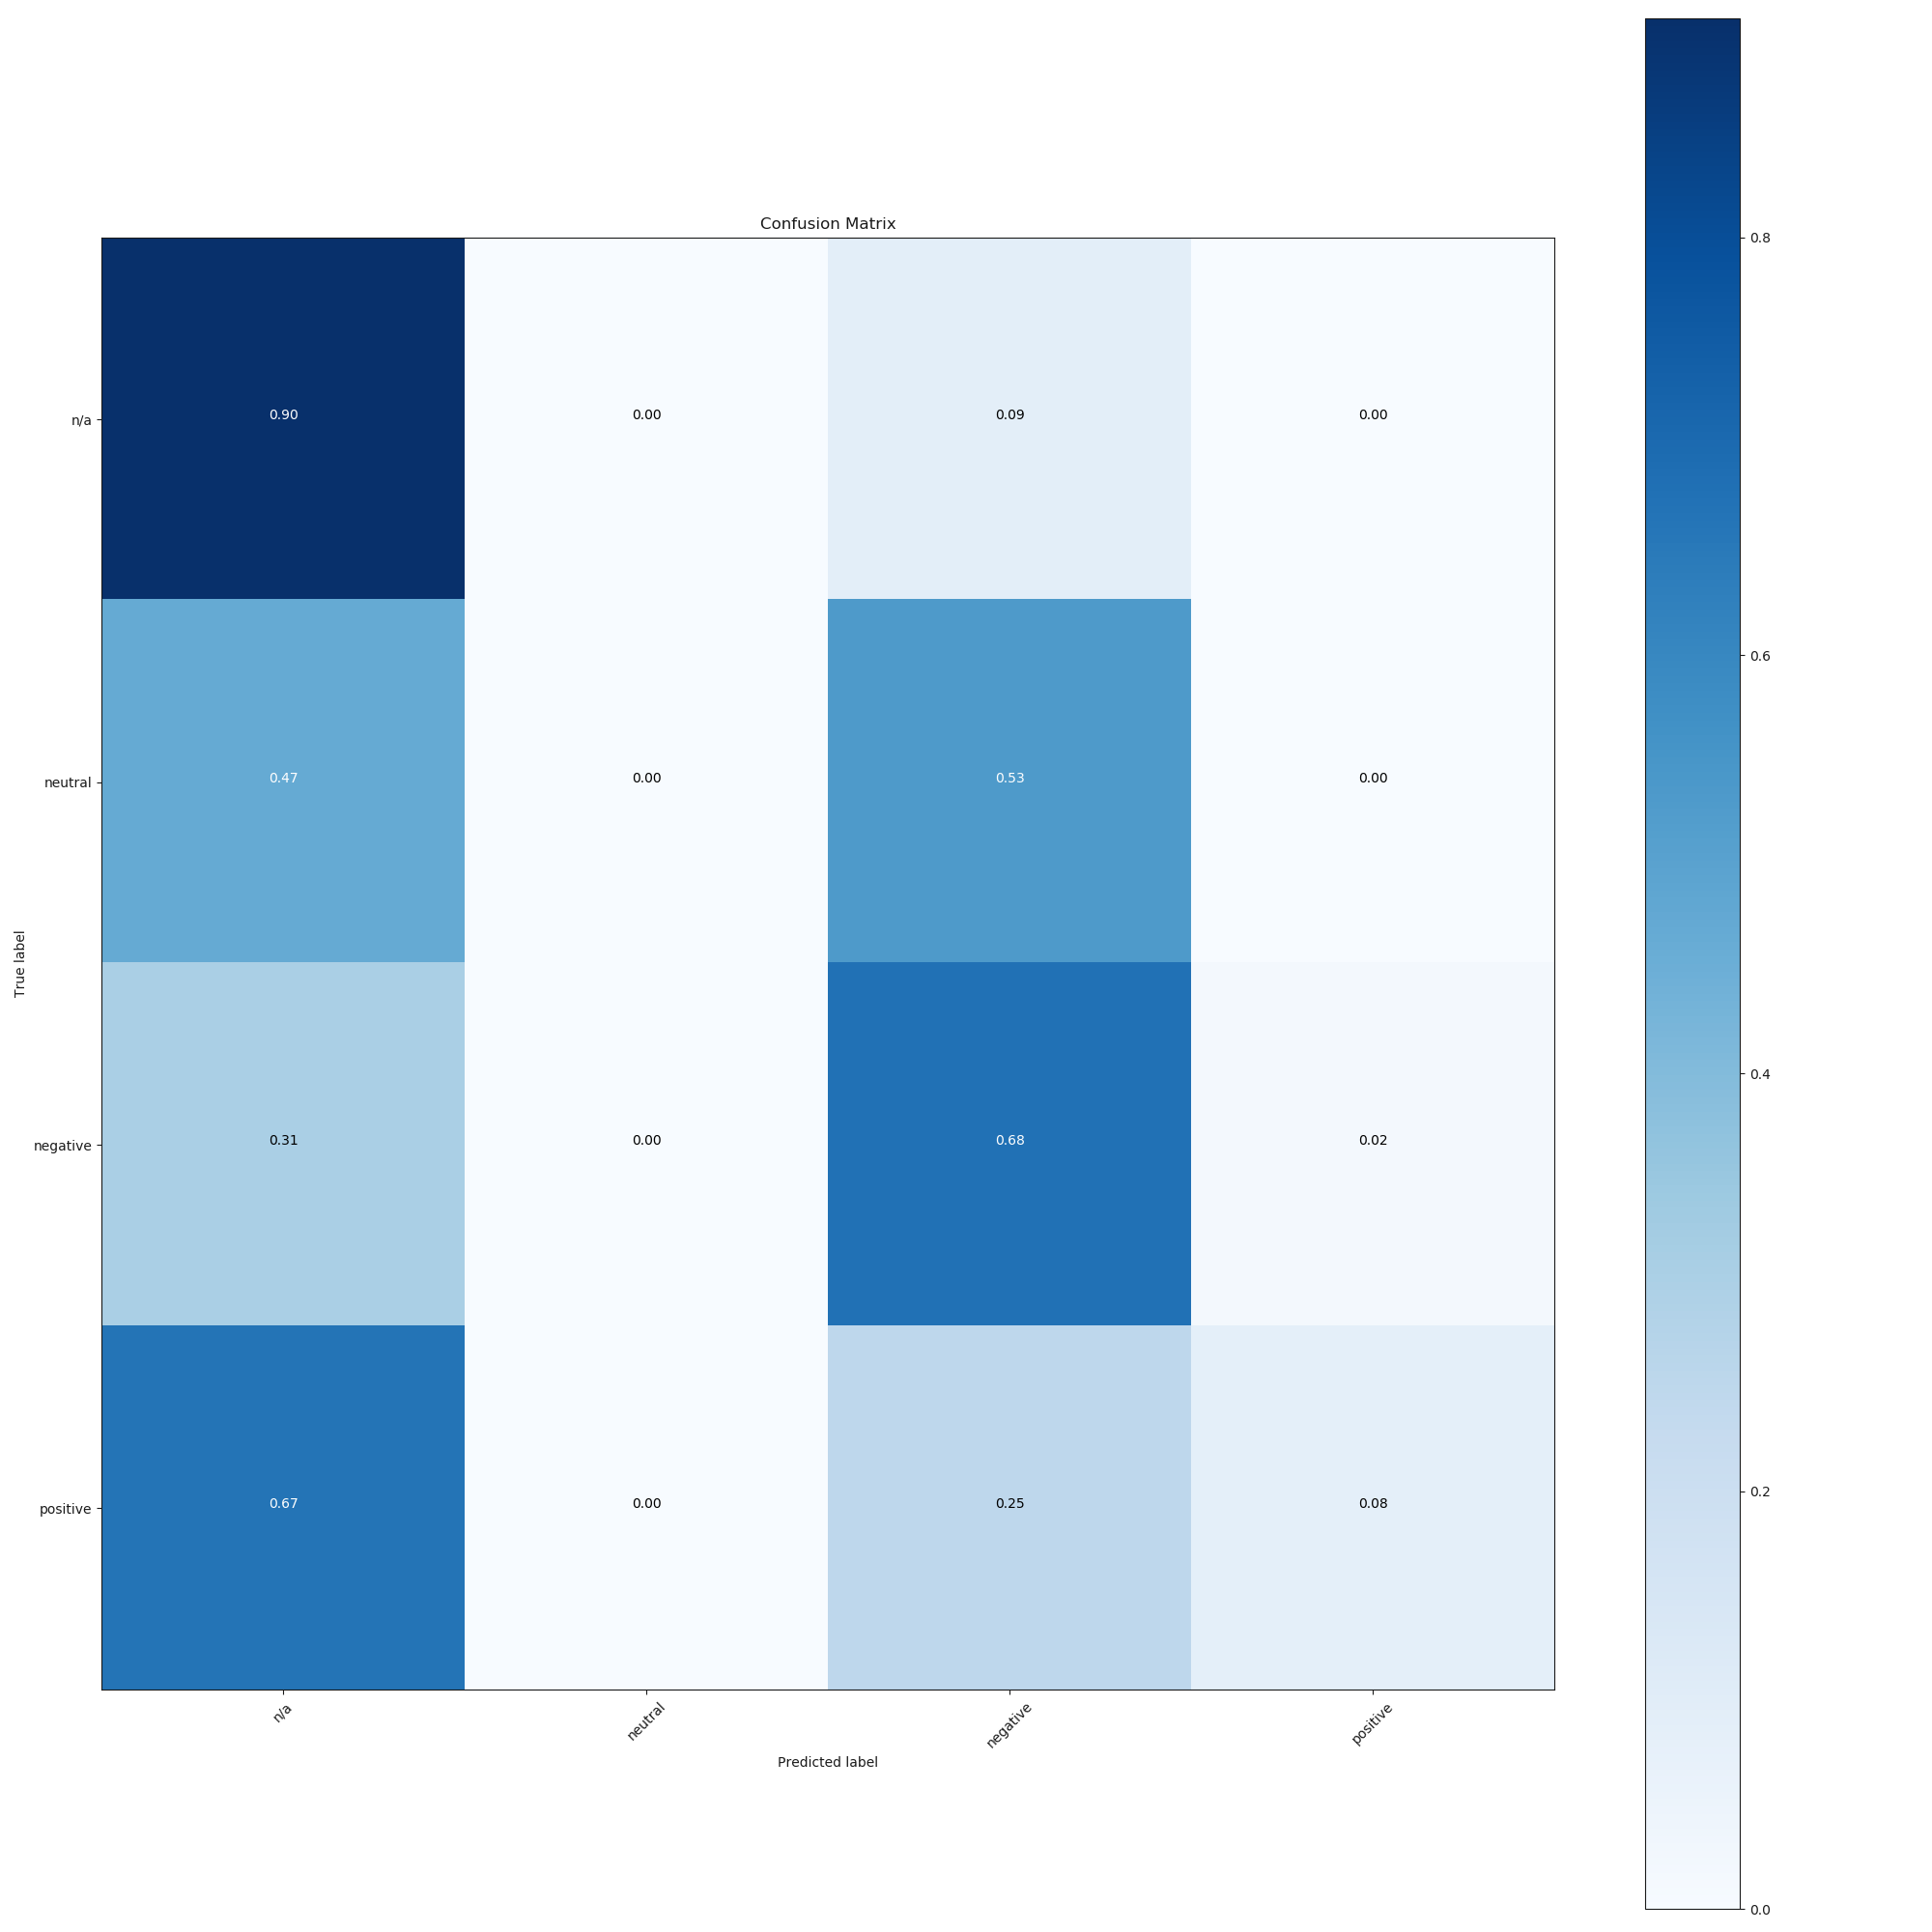
\includegraphics[width=0.19\textwidth]{figures/08_appendix/germeval/08_2}
    }
    \subfloat[Auslastung + Platz]{
        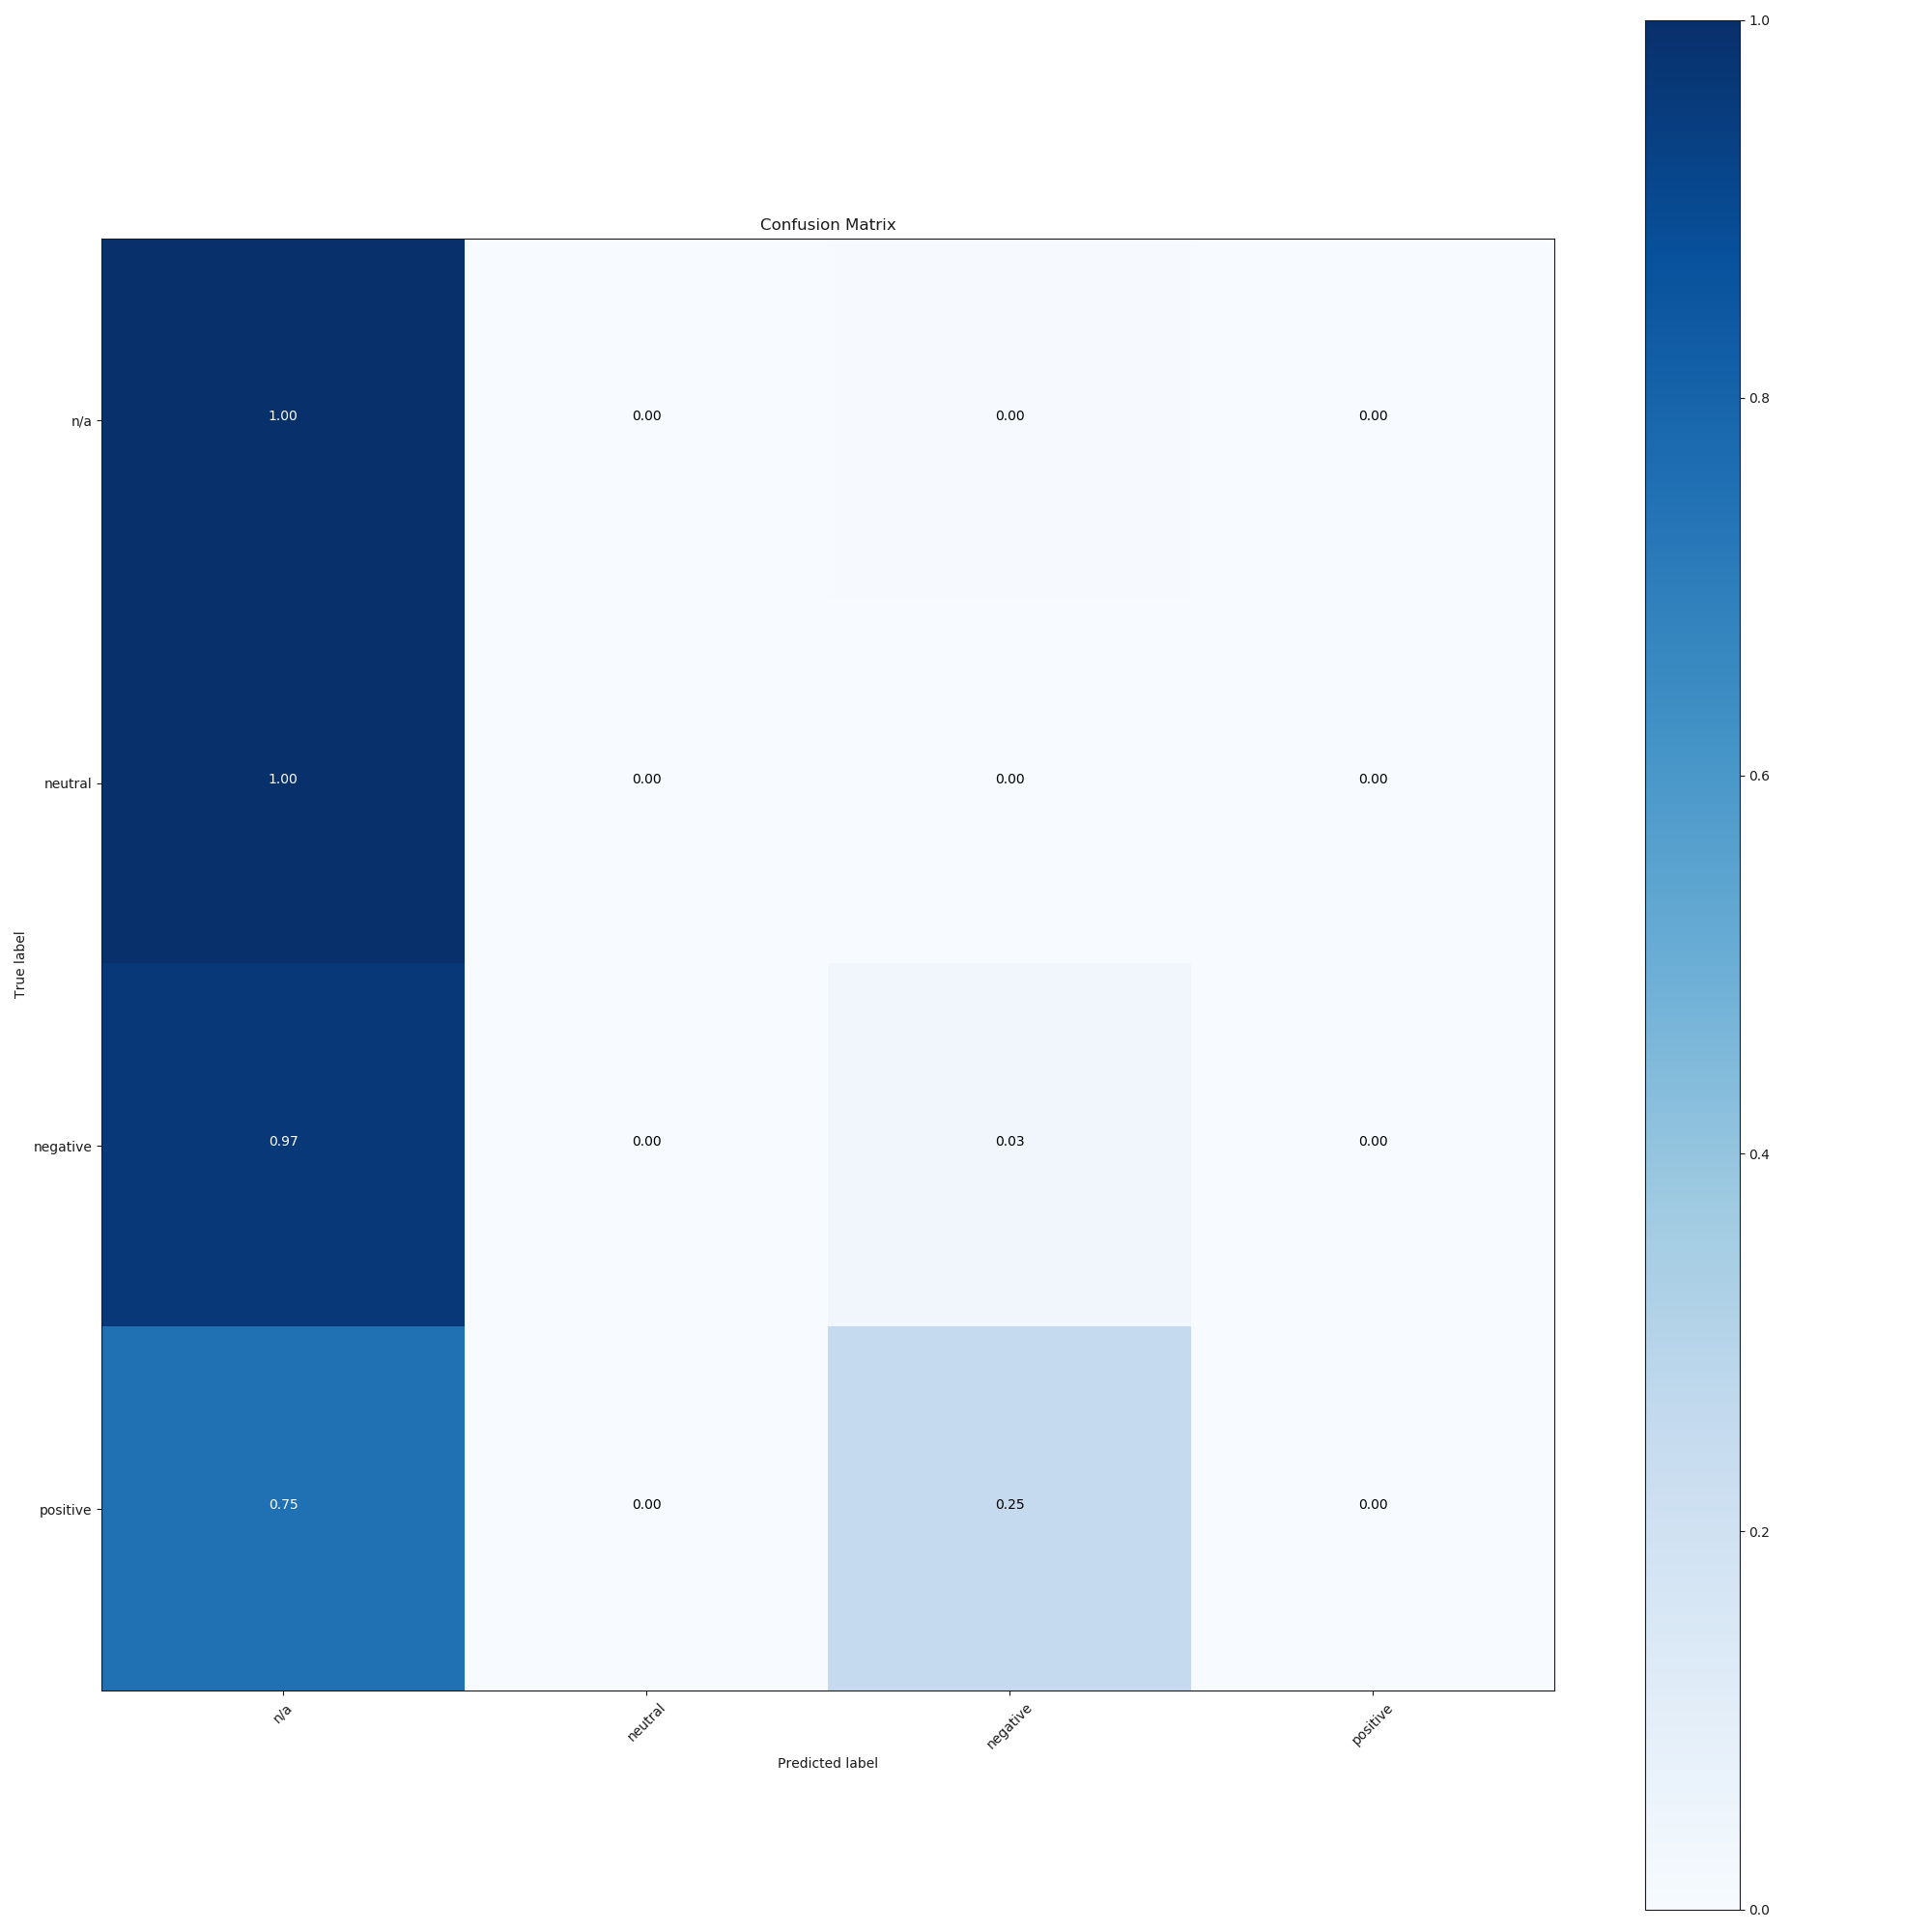
\includegraphics[width=0.19\textwidth]{figures/08_appendix/germeval/08_3}
    }
    \subfloat[Barrierefreiheit]{
        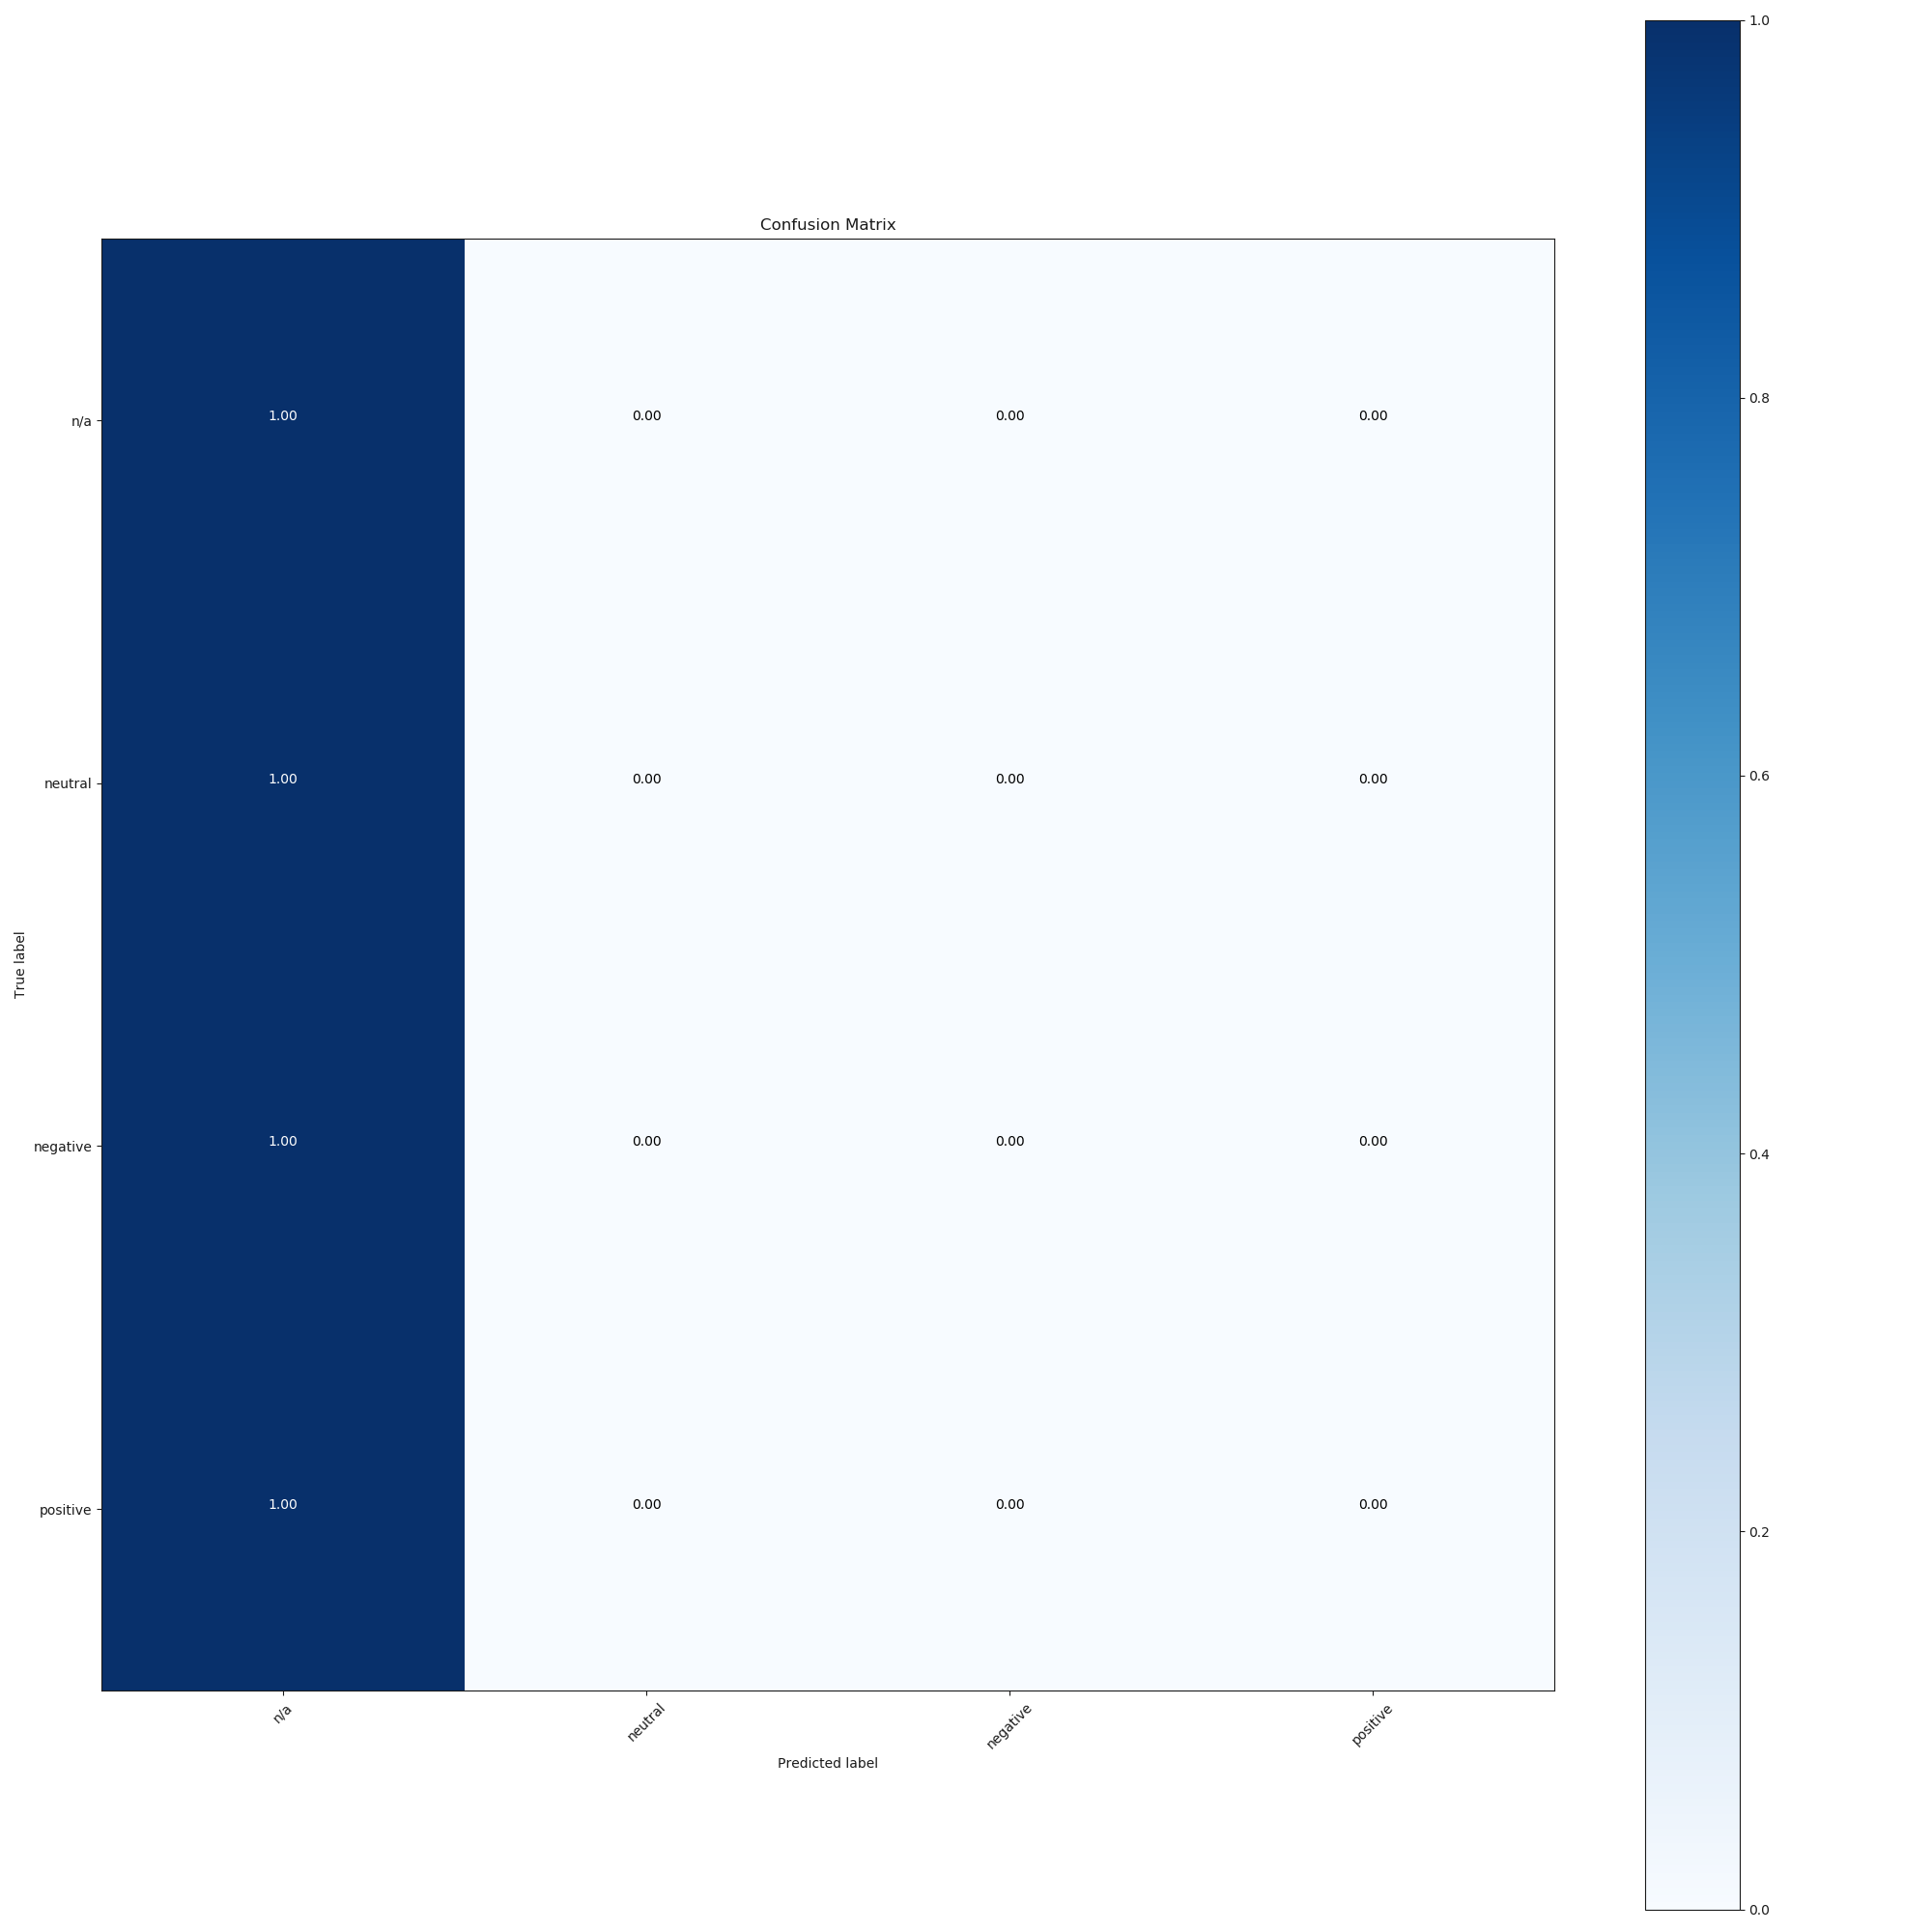
\includegraphics[width=0.19\textwidth]{figures/08_appendix/germeval/08_4}
    }
    \subfloat[Connectivity]{
        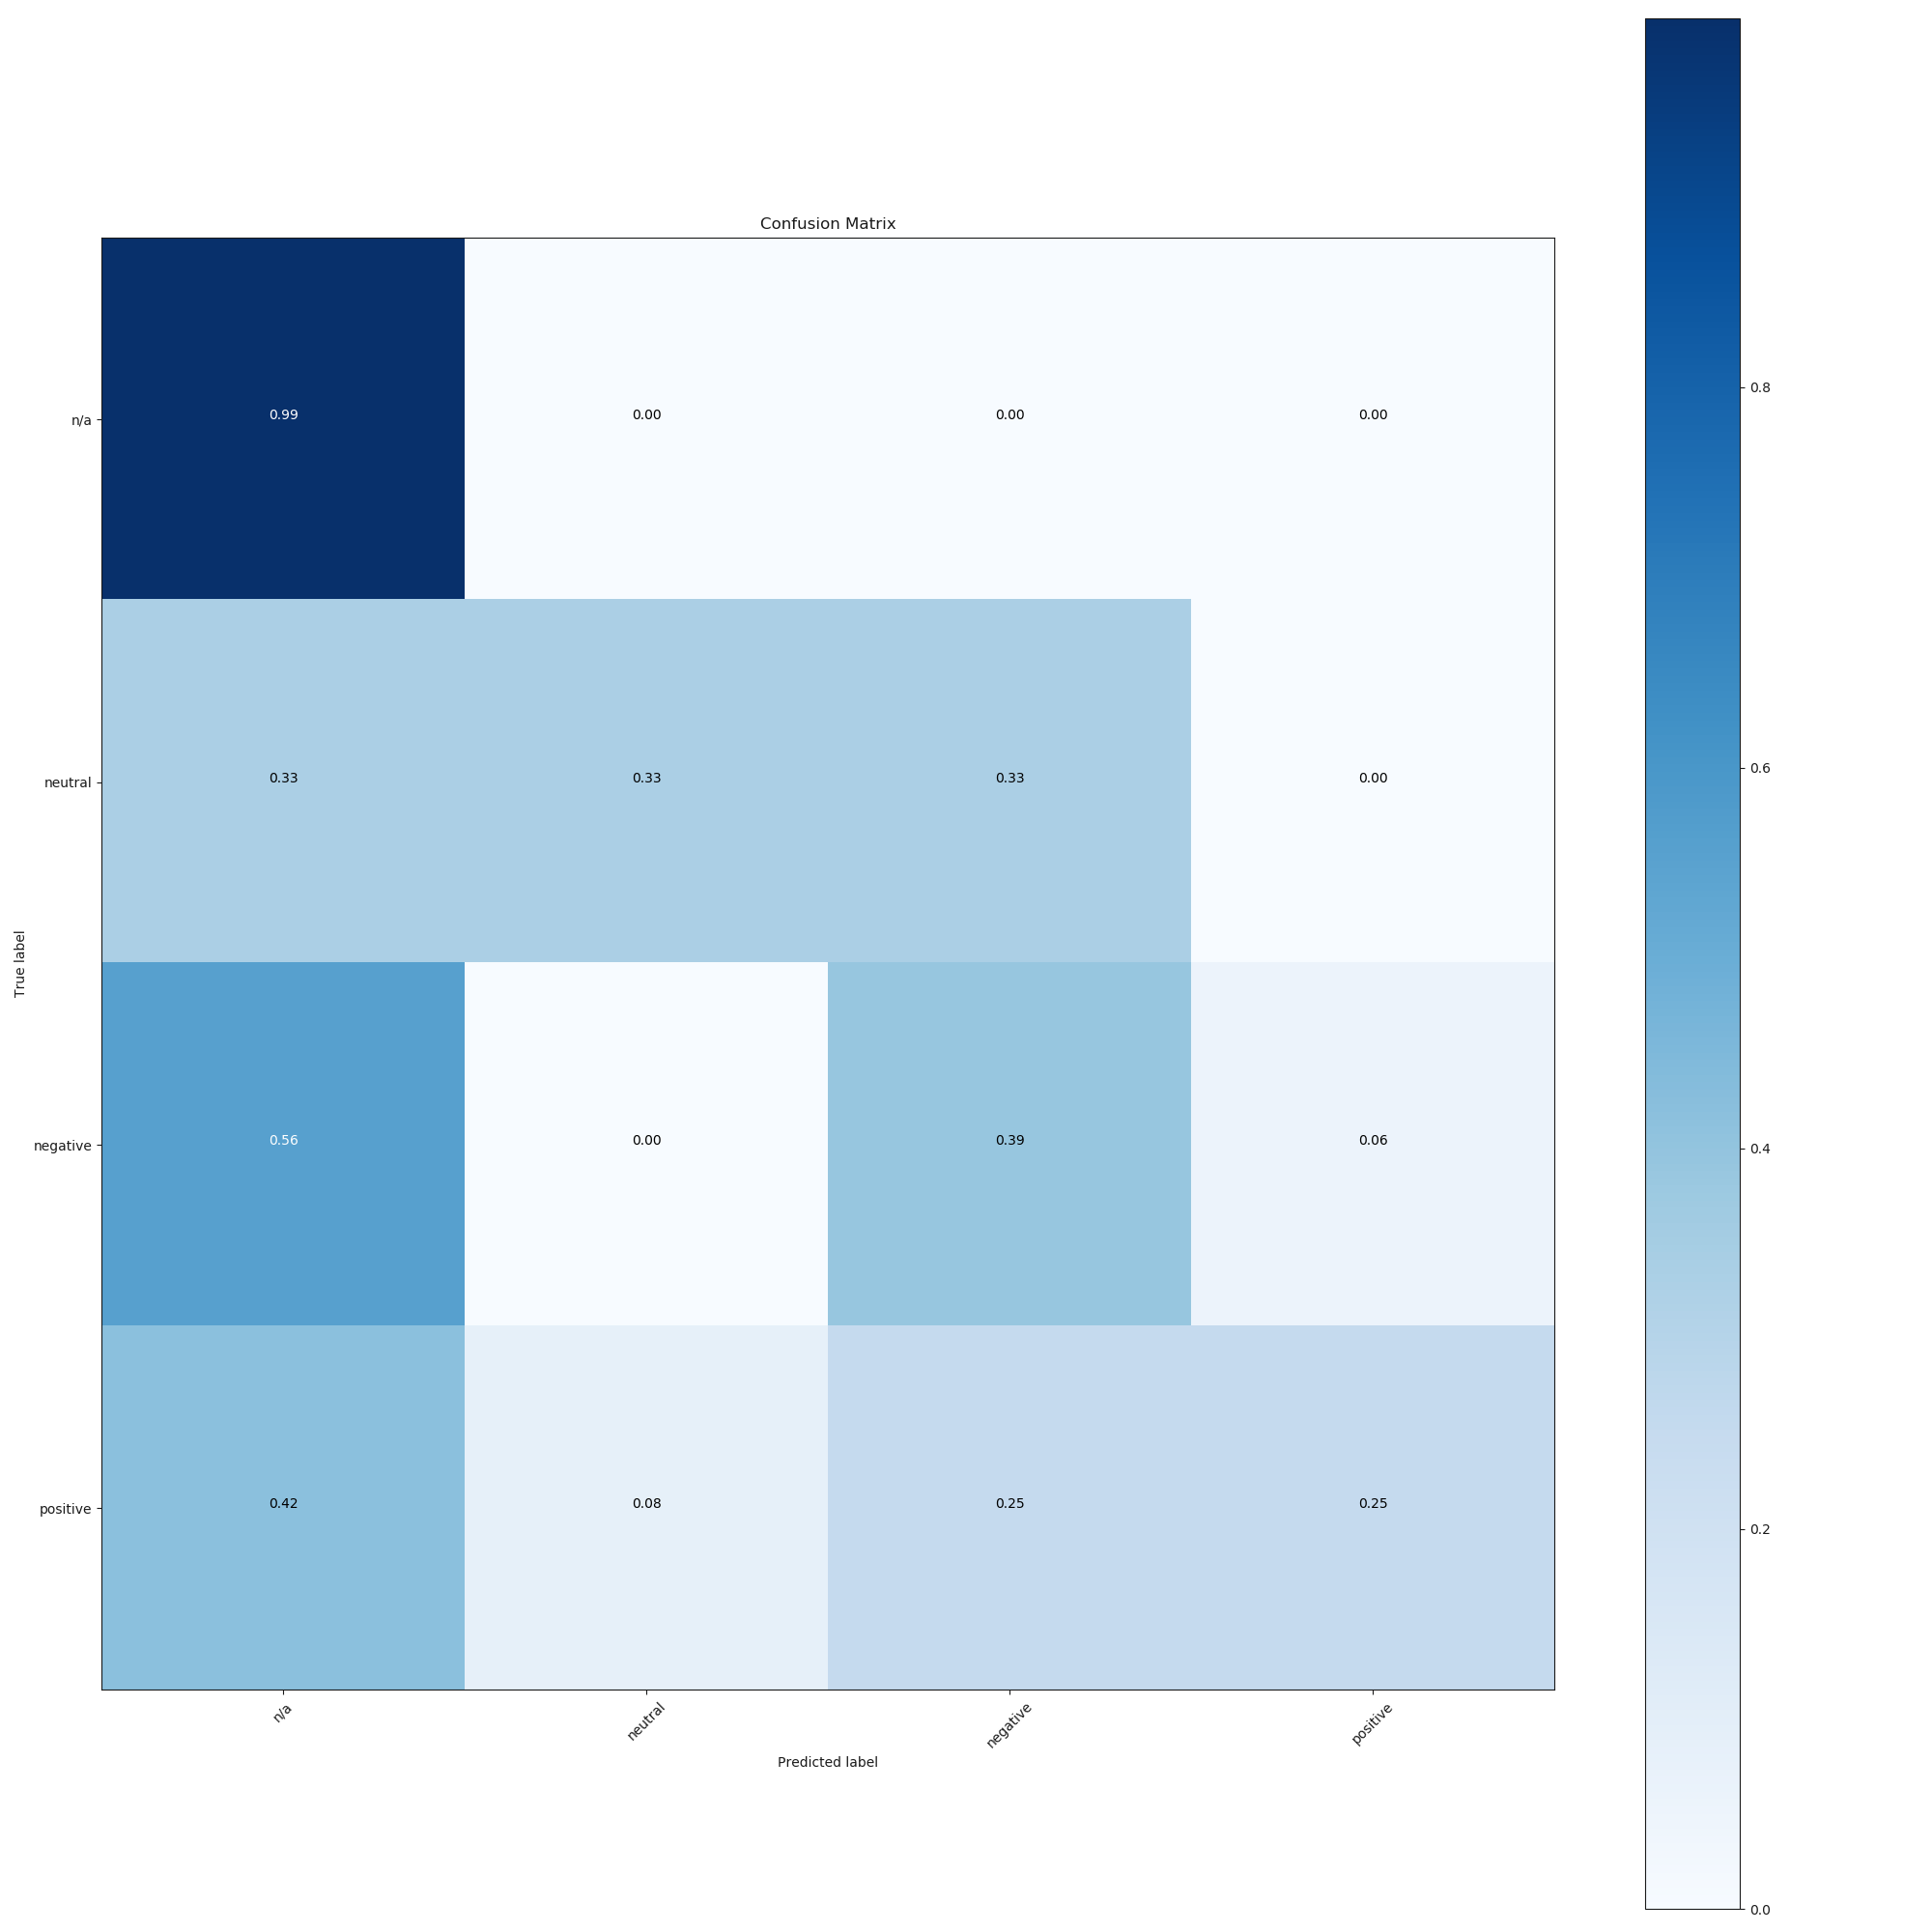
\includegraphics[width=0.19\textwidth]{figures/08_appendix/germeval/08_5}
    }     
    \hspace{0mm}

    \subfloat[App \& Website]{
        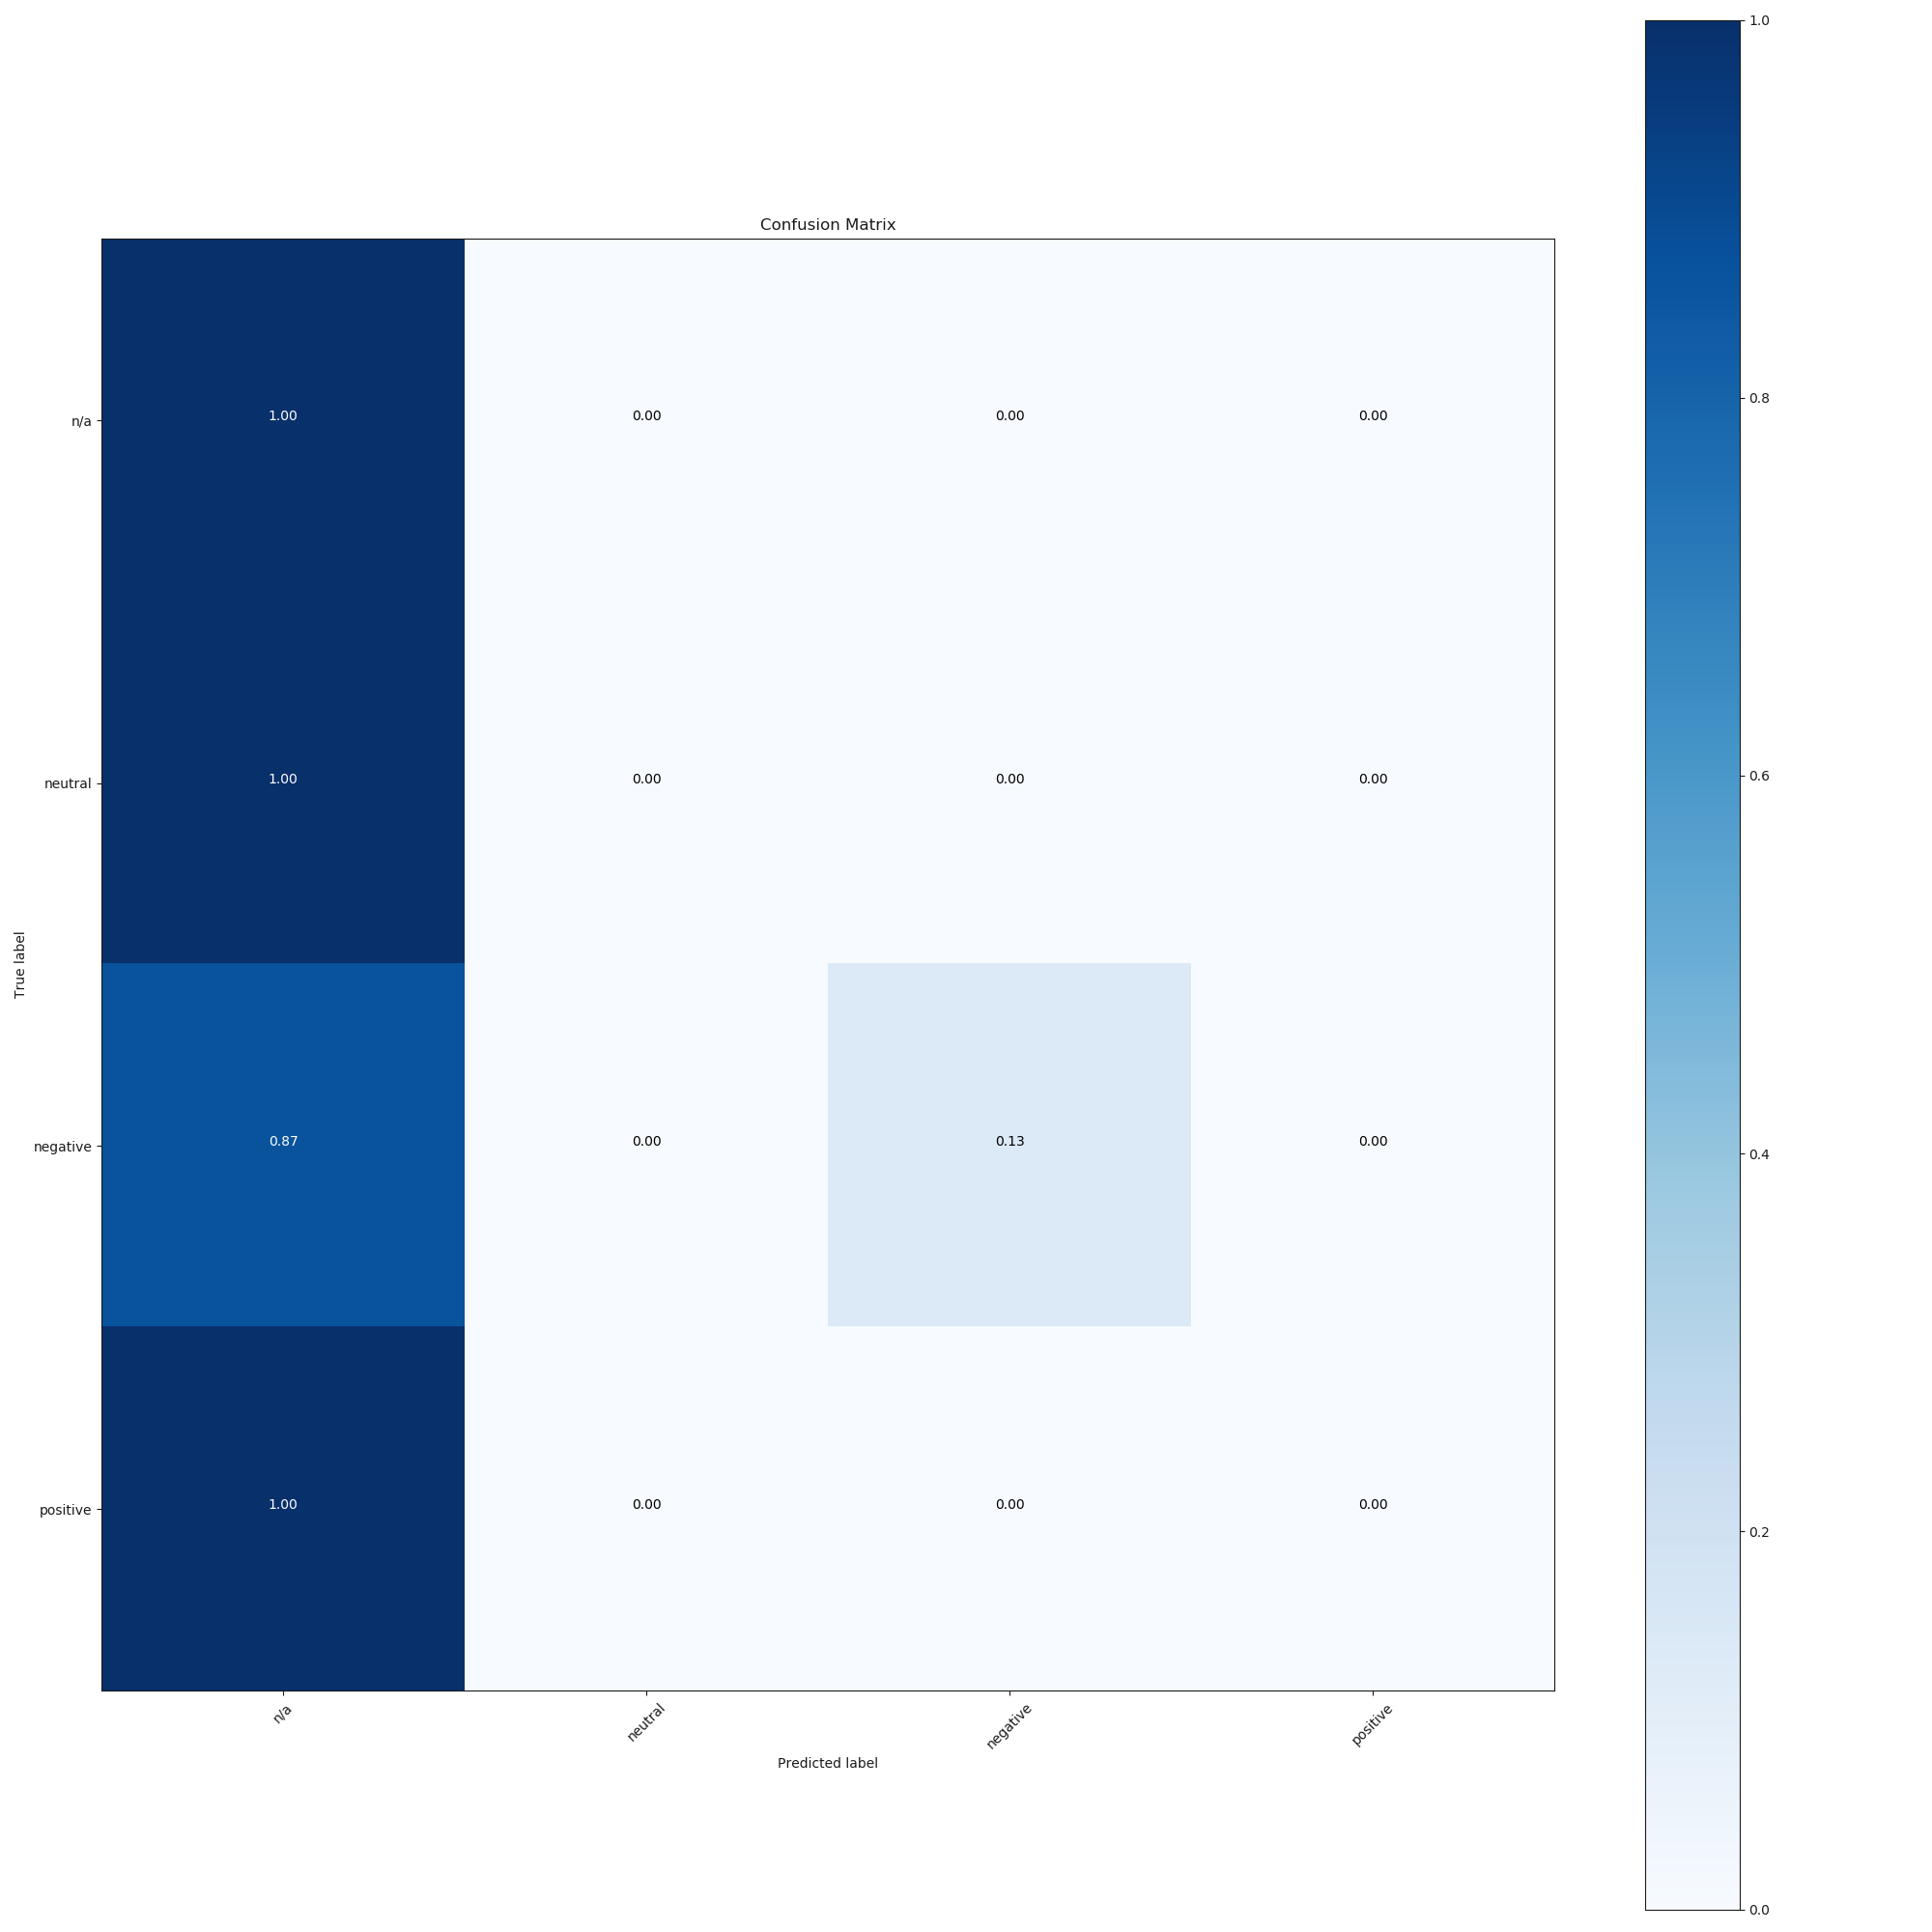
\includegraphics[width=0.19\textwidth]{figures/08_appendix/germeval/08_6}
    }
    \subfloat[Design]{
        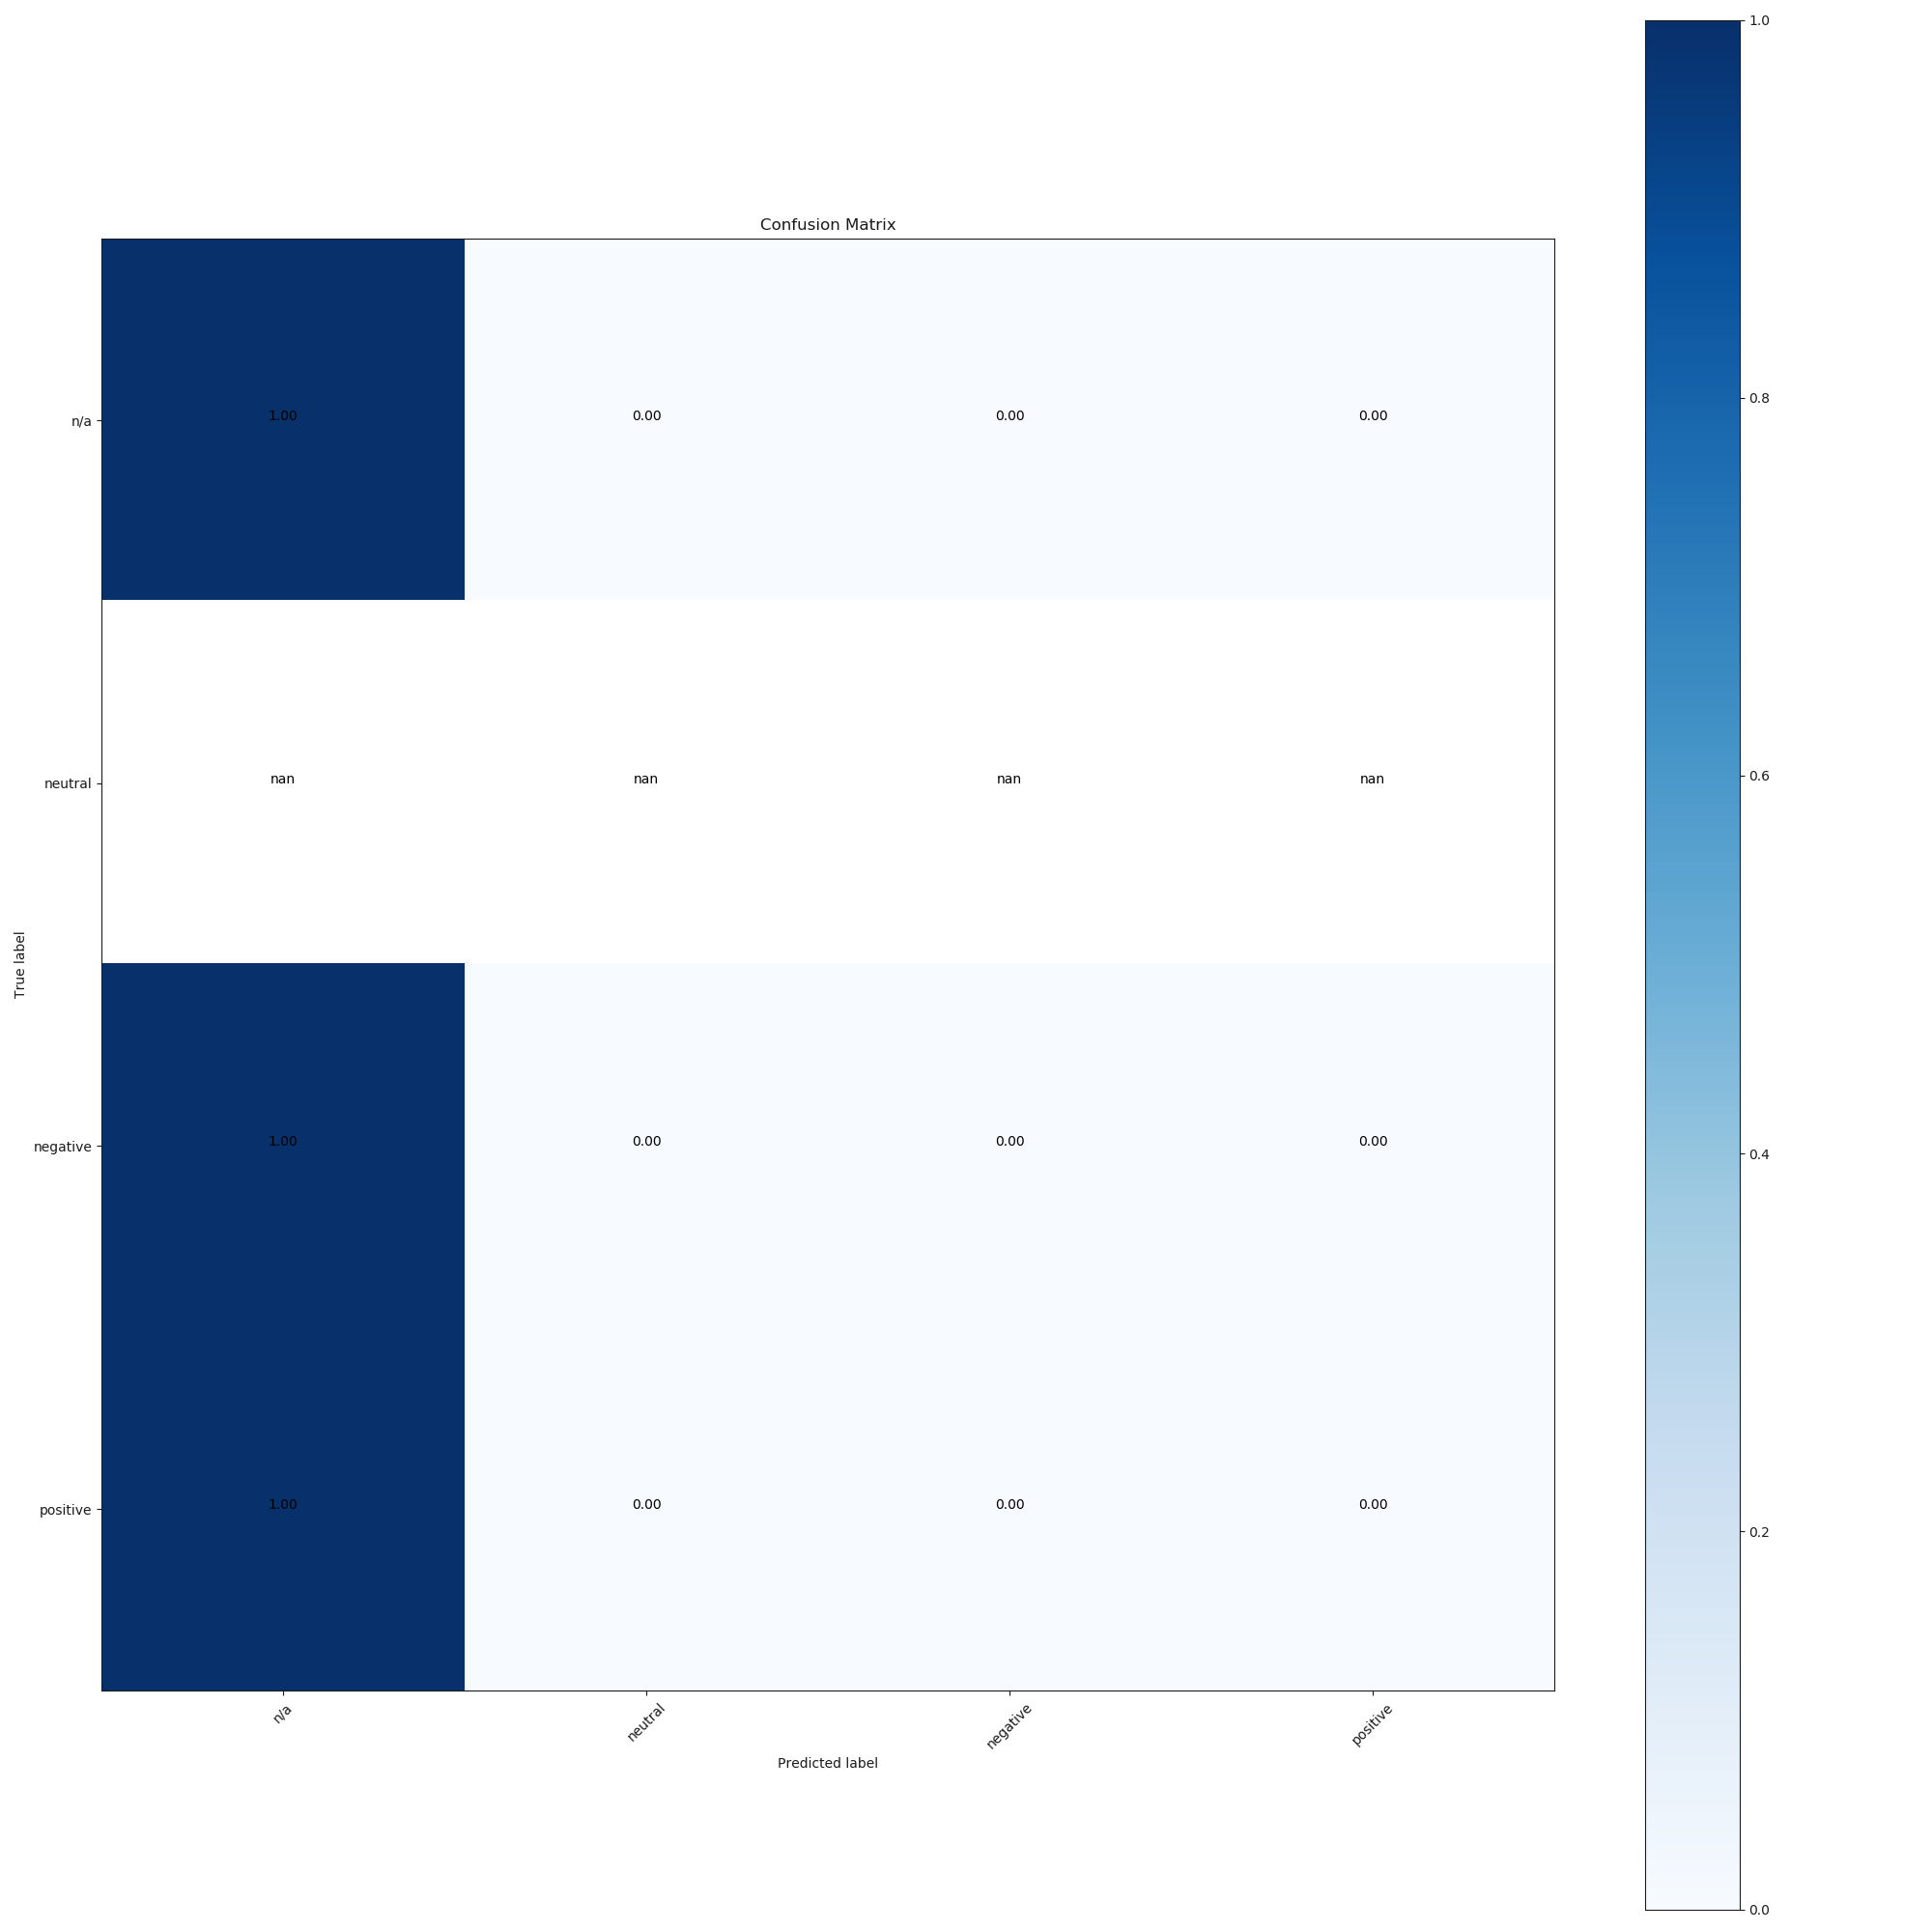
\includegraphics[width=0.19\textwidth]{figures/08_appendix/germeval/08_7}
    }
    \subfloat[Gastronomie]{
        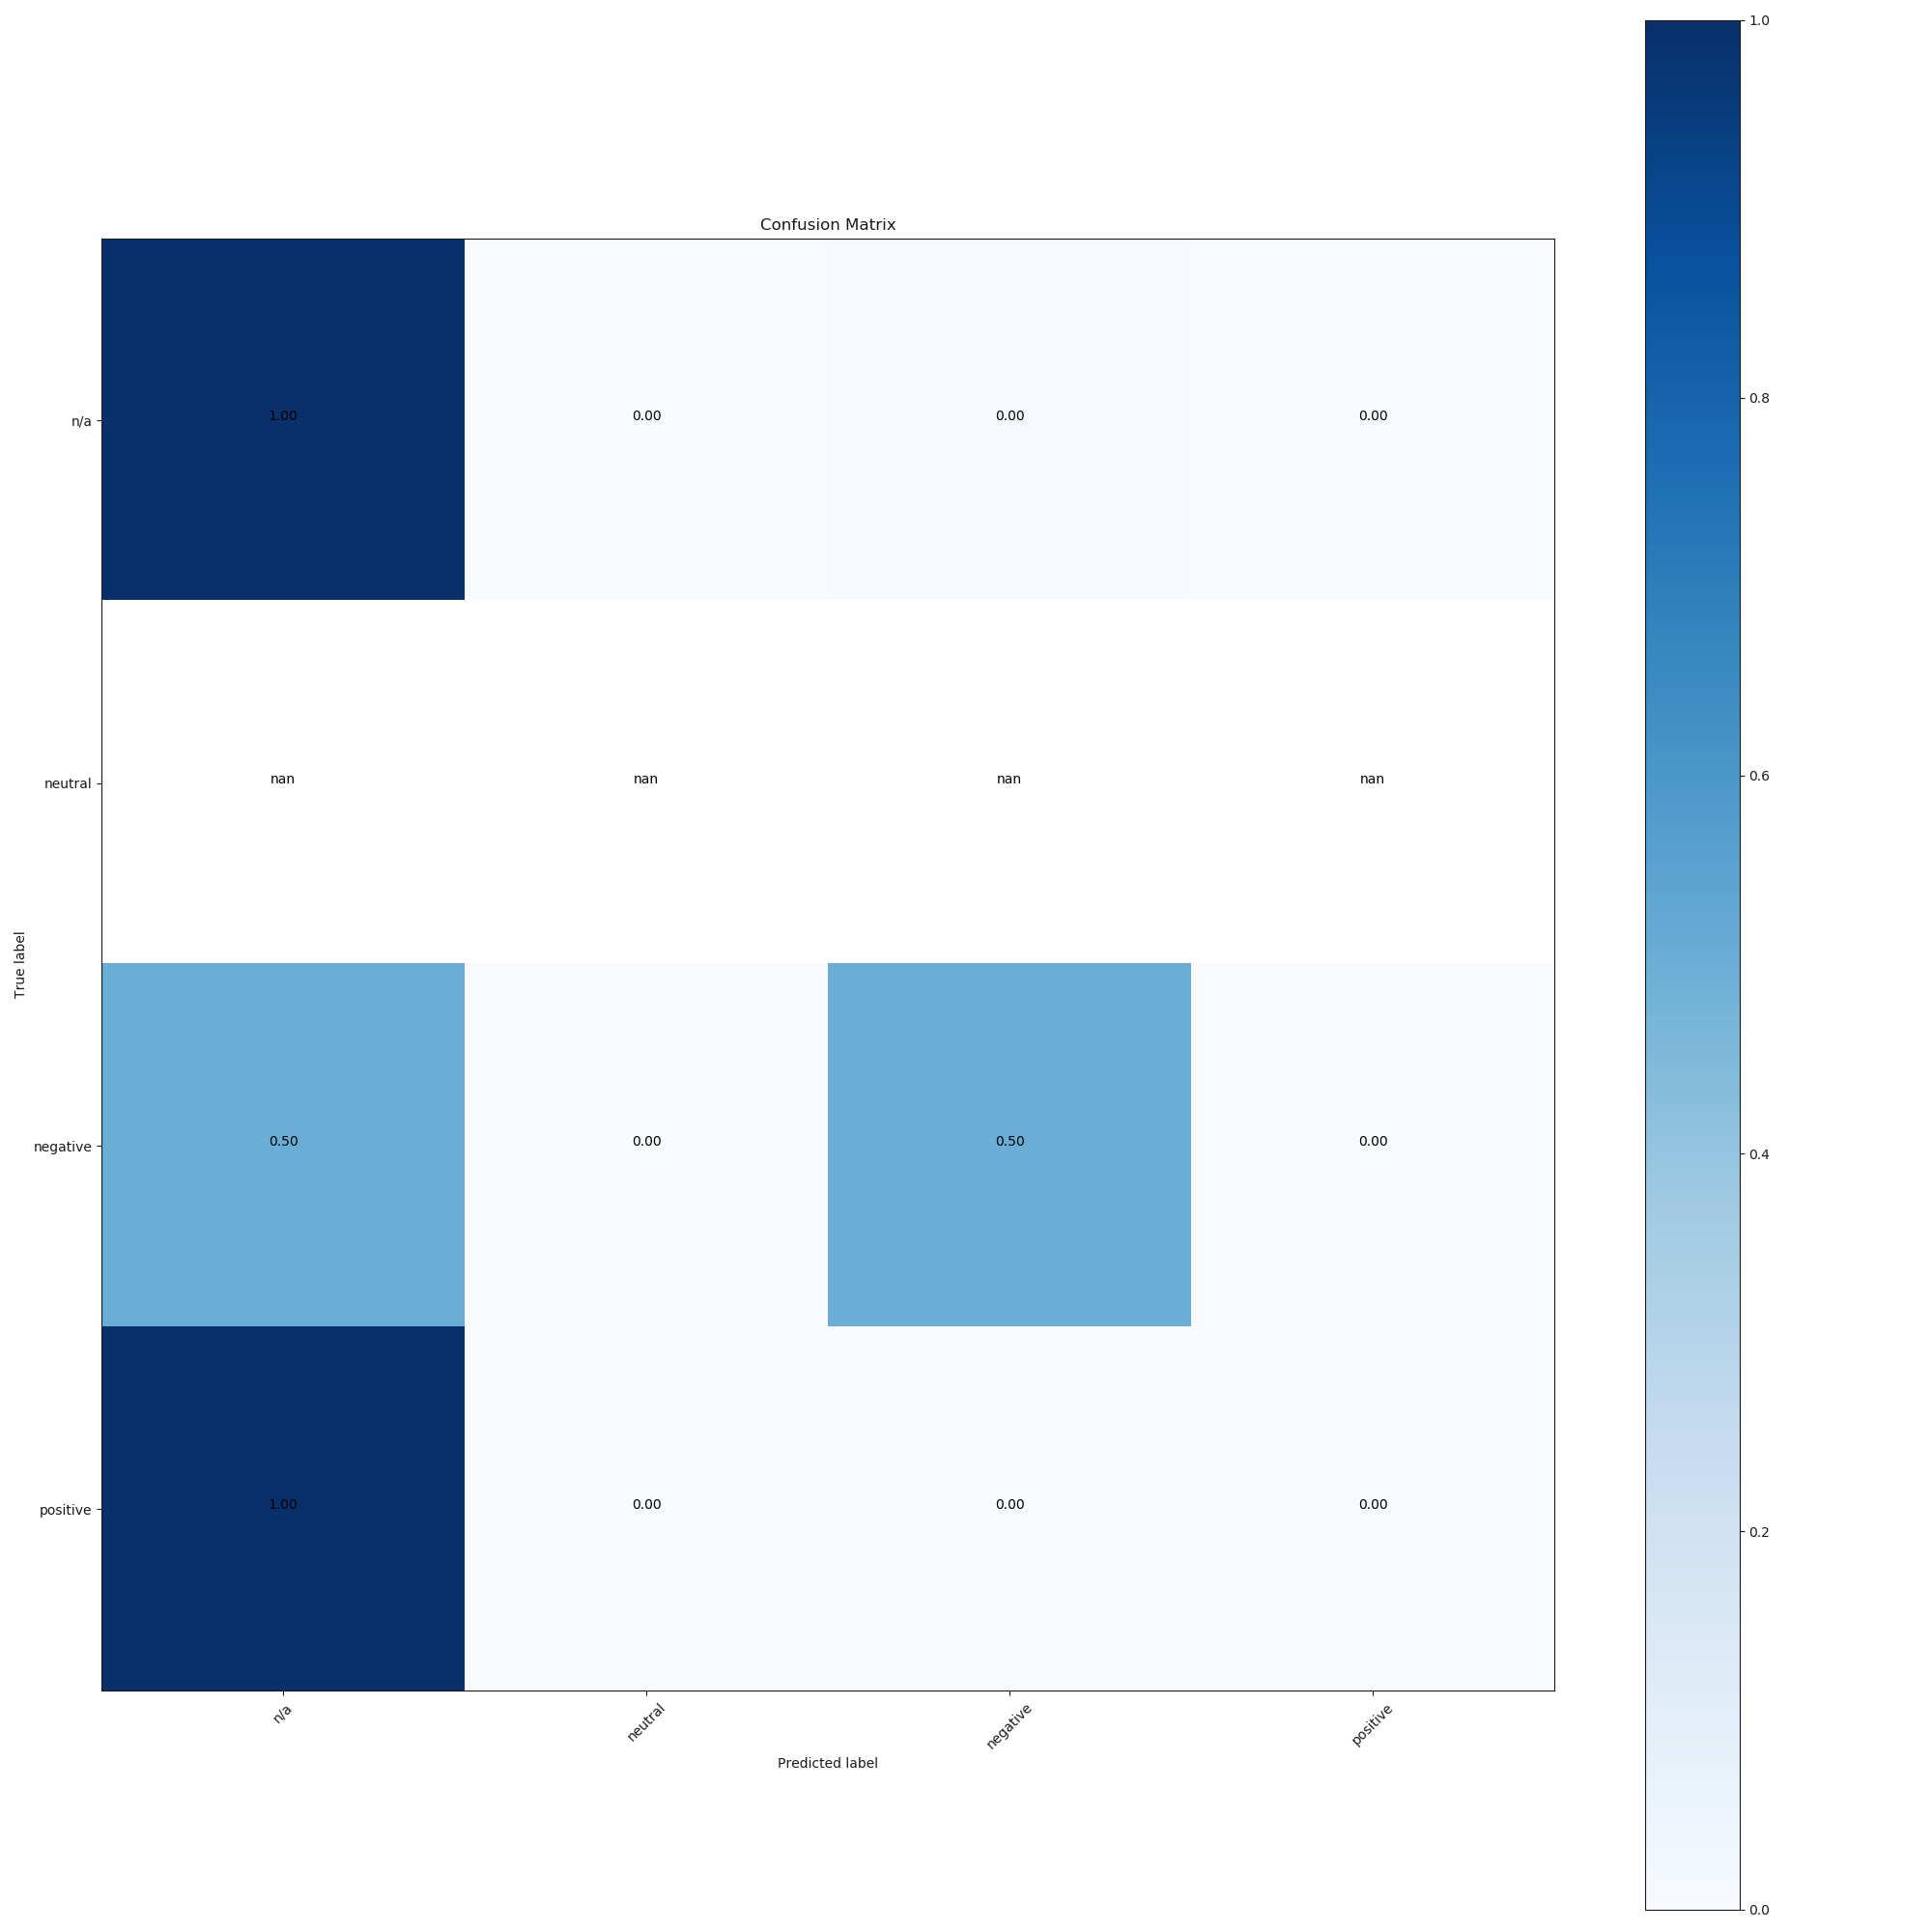
\includegraphics[width=0.19\textwidth]{figures/08_appendix/germeval/08_8}
    }
    \subfloat[Gepäck]{
        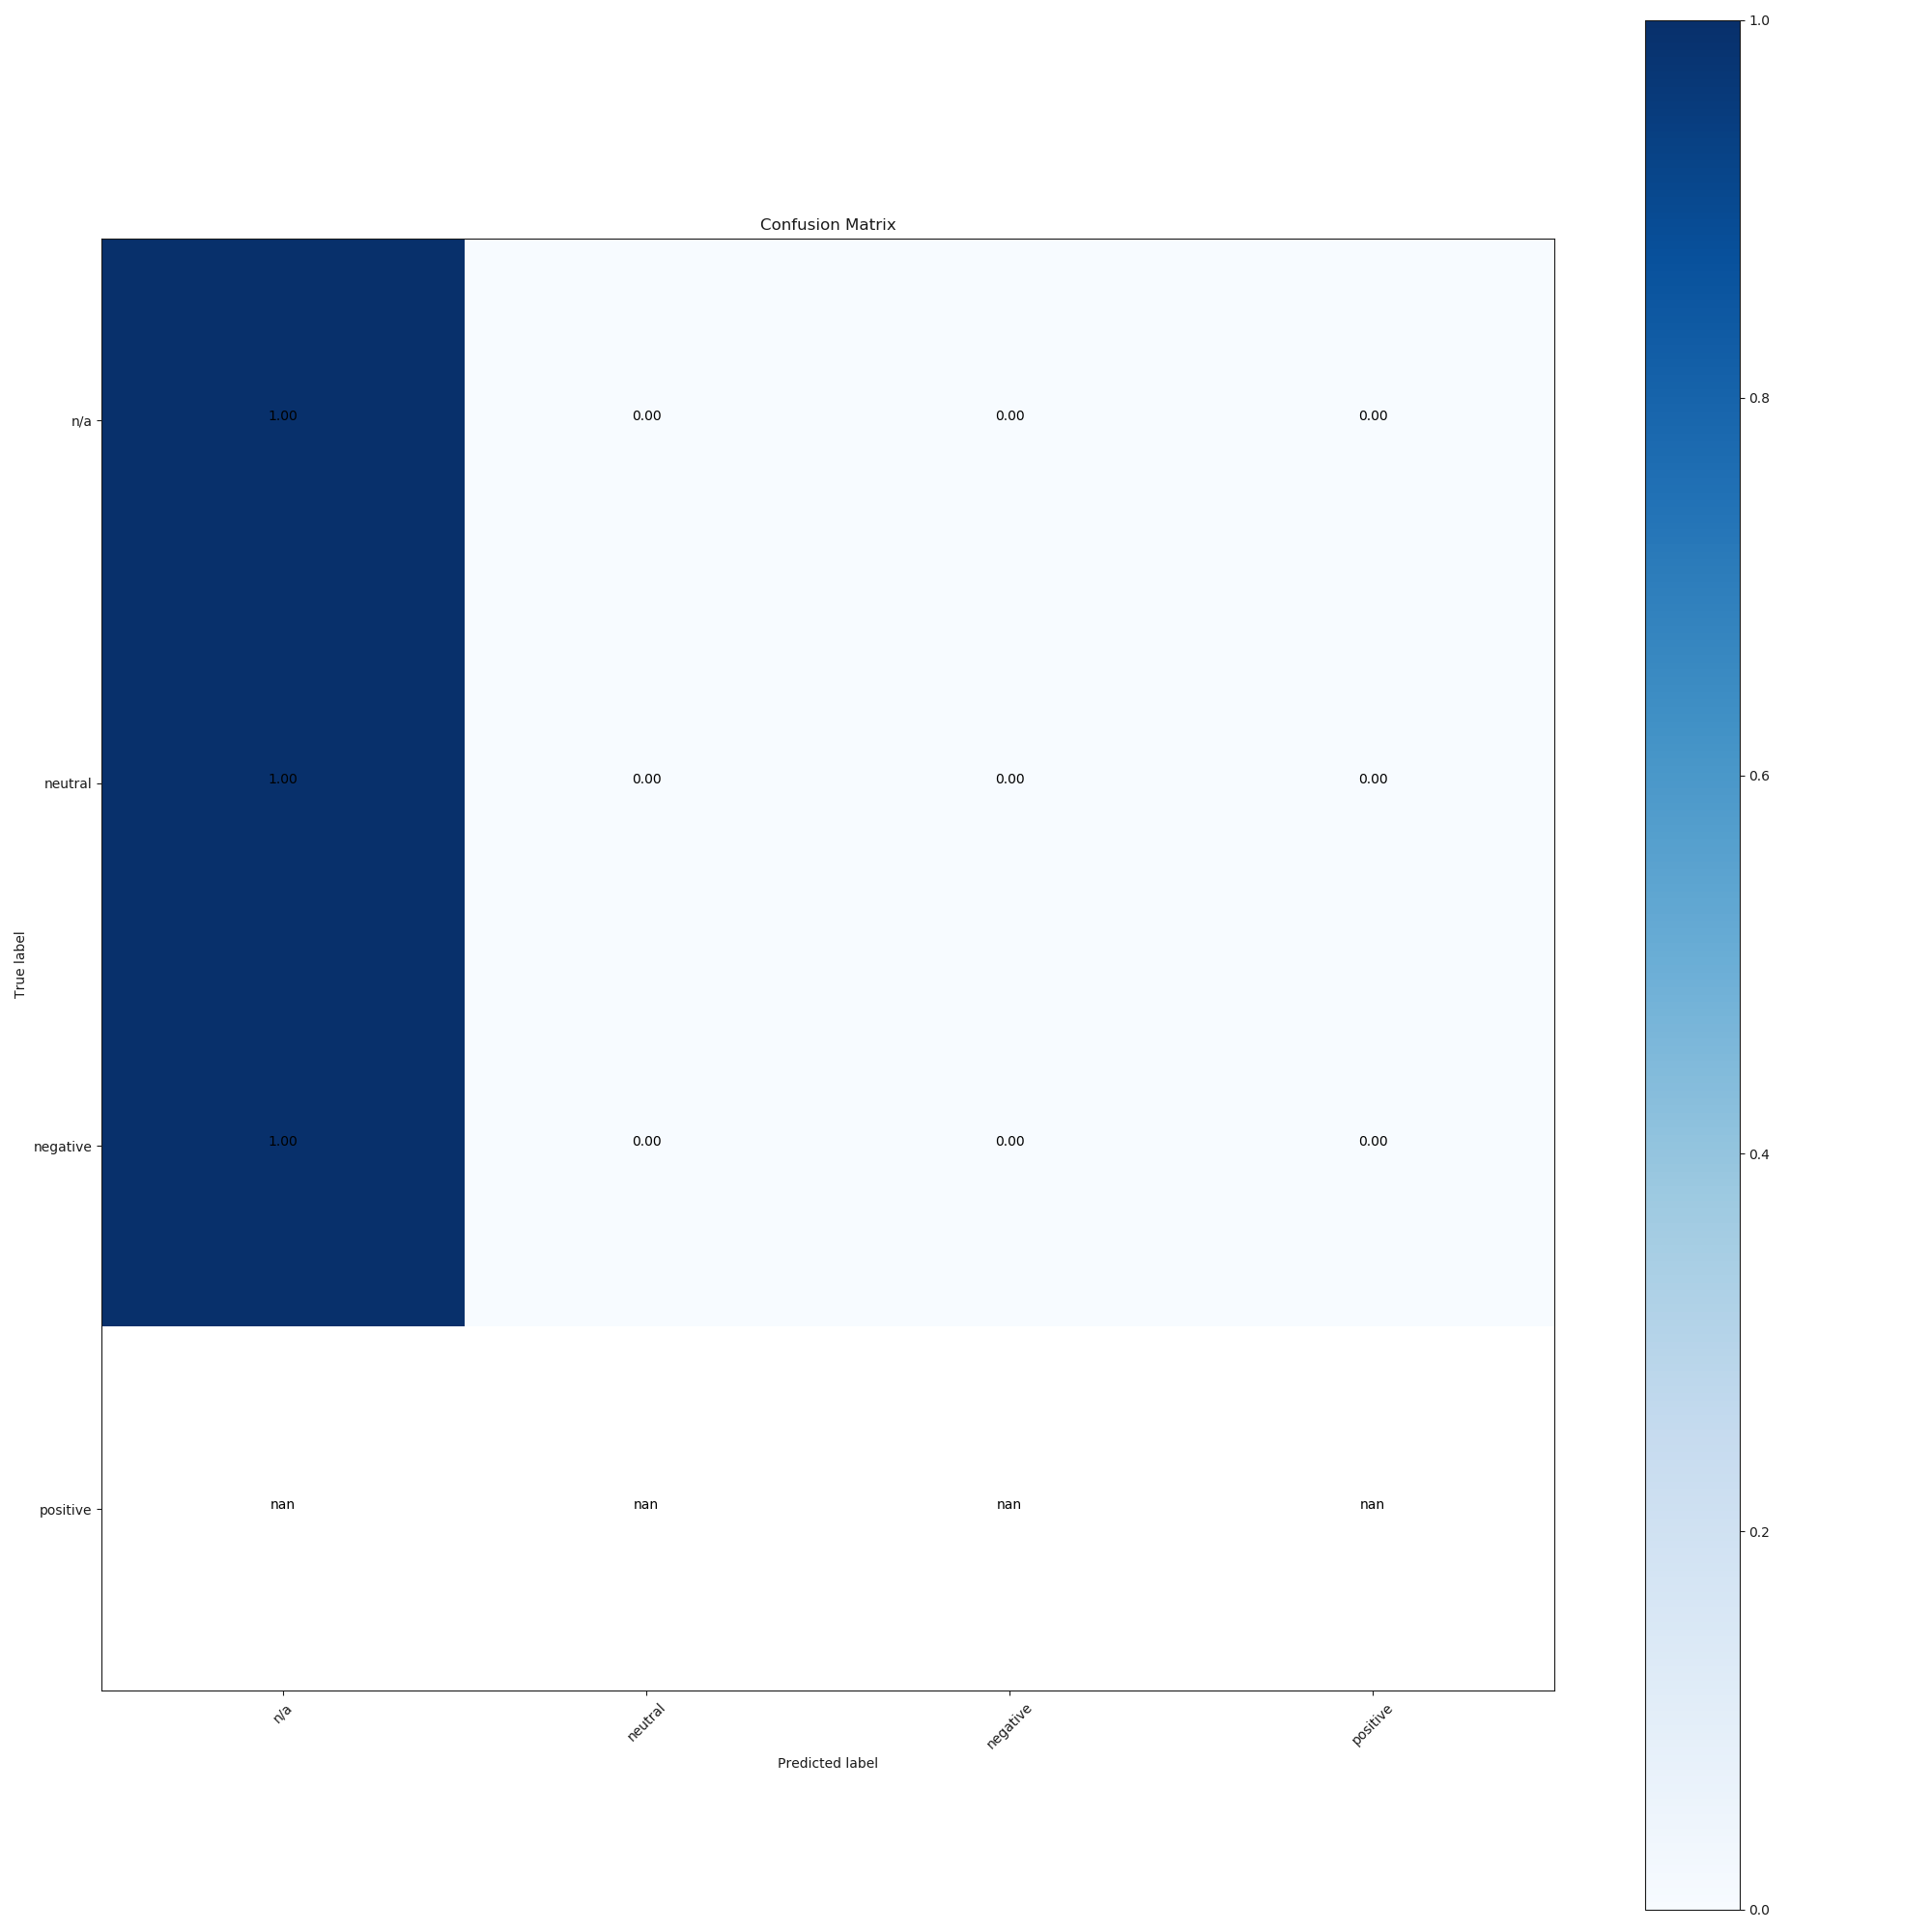
\includegraphics[width=0.19\textwidth]{figures/08_appendix/germeval/08_9}
    }
    \subfloat[Image]{
        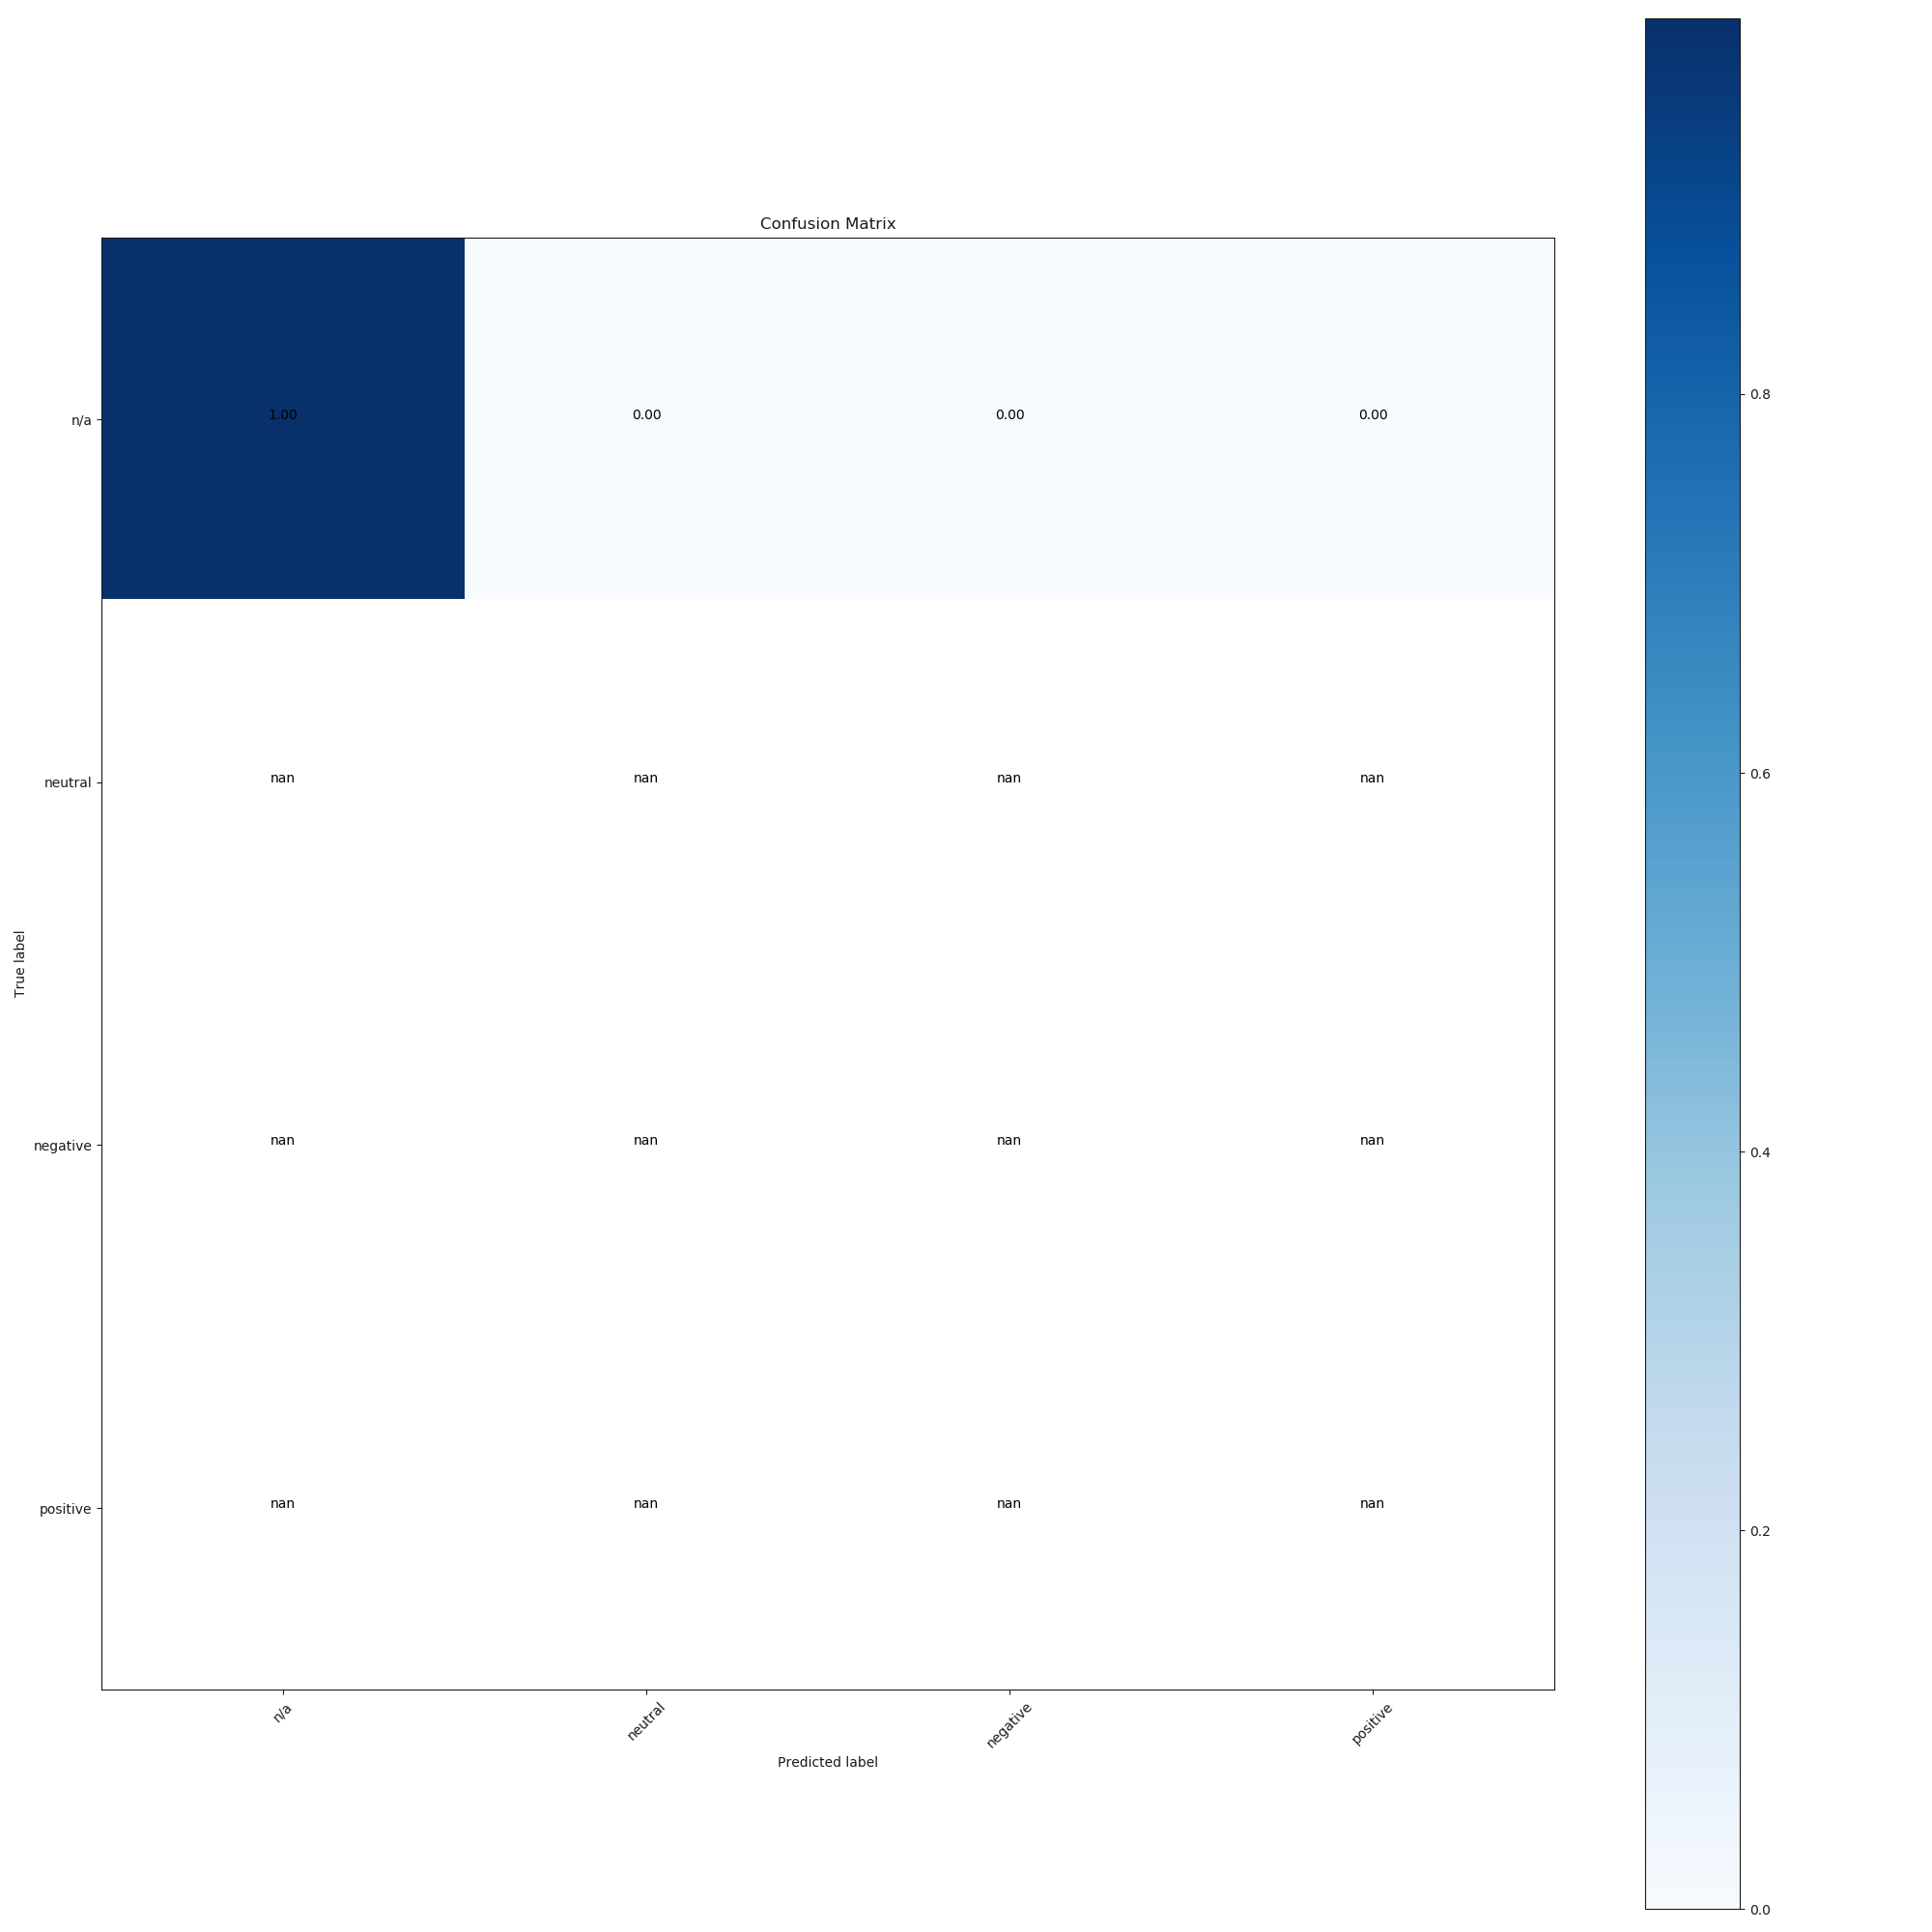
\includegraphics[width=0.19\textwidth]{figures/08_appendix/germeval/08_10}
    }
    \hspace{0mm}

    \subfloat[Informationen]{
        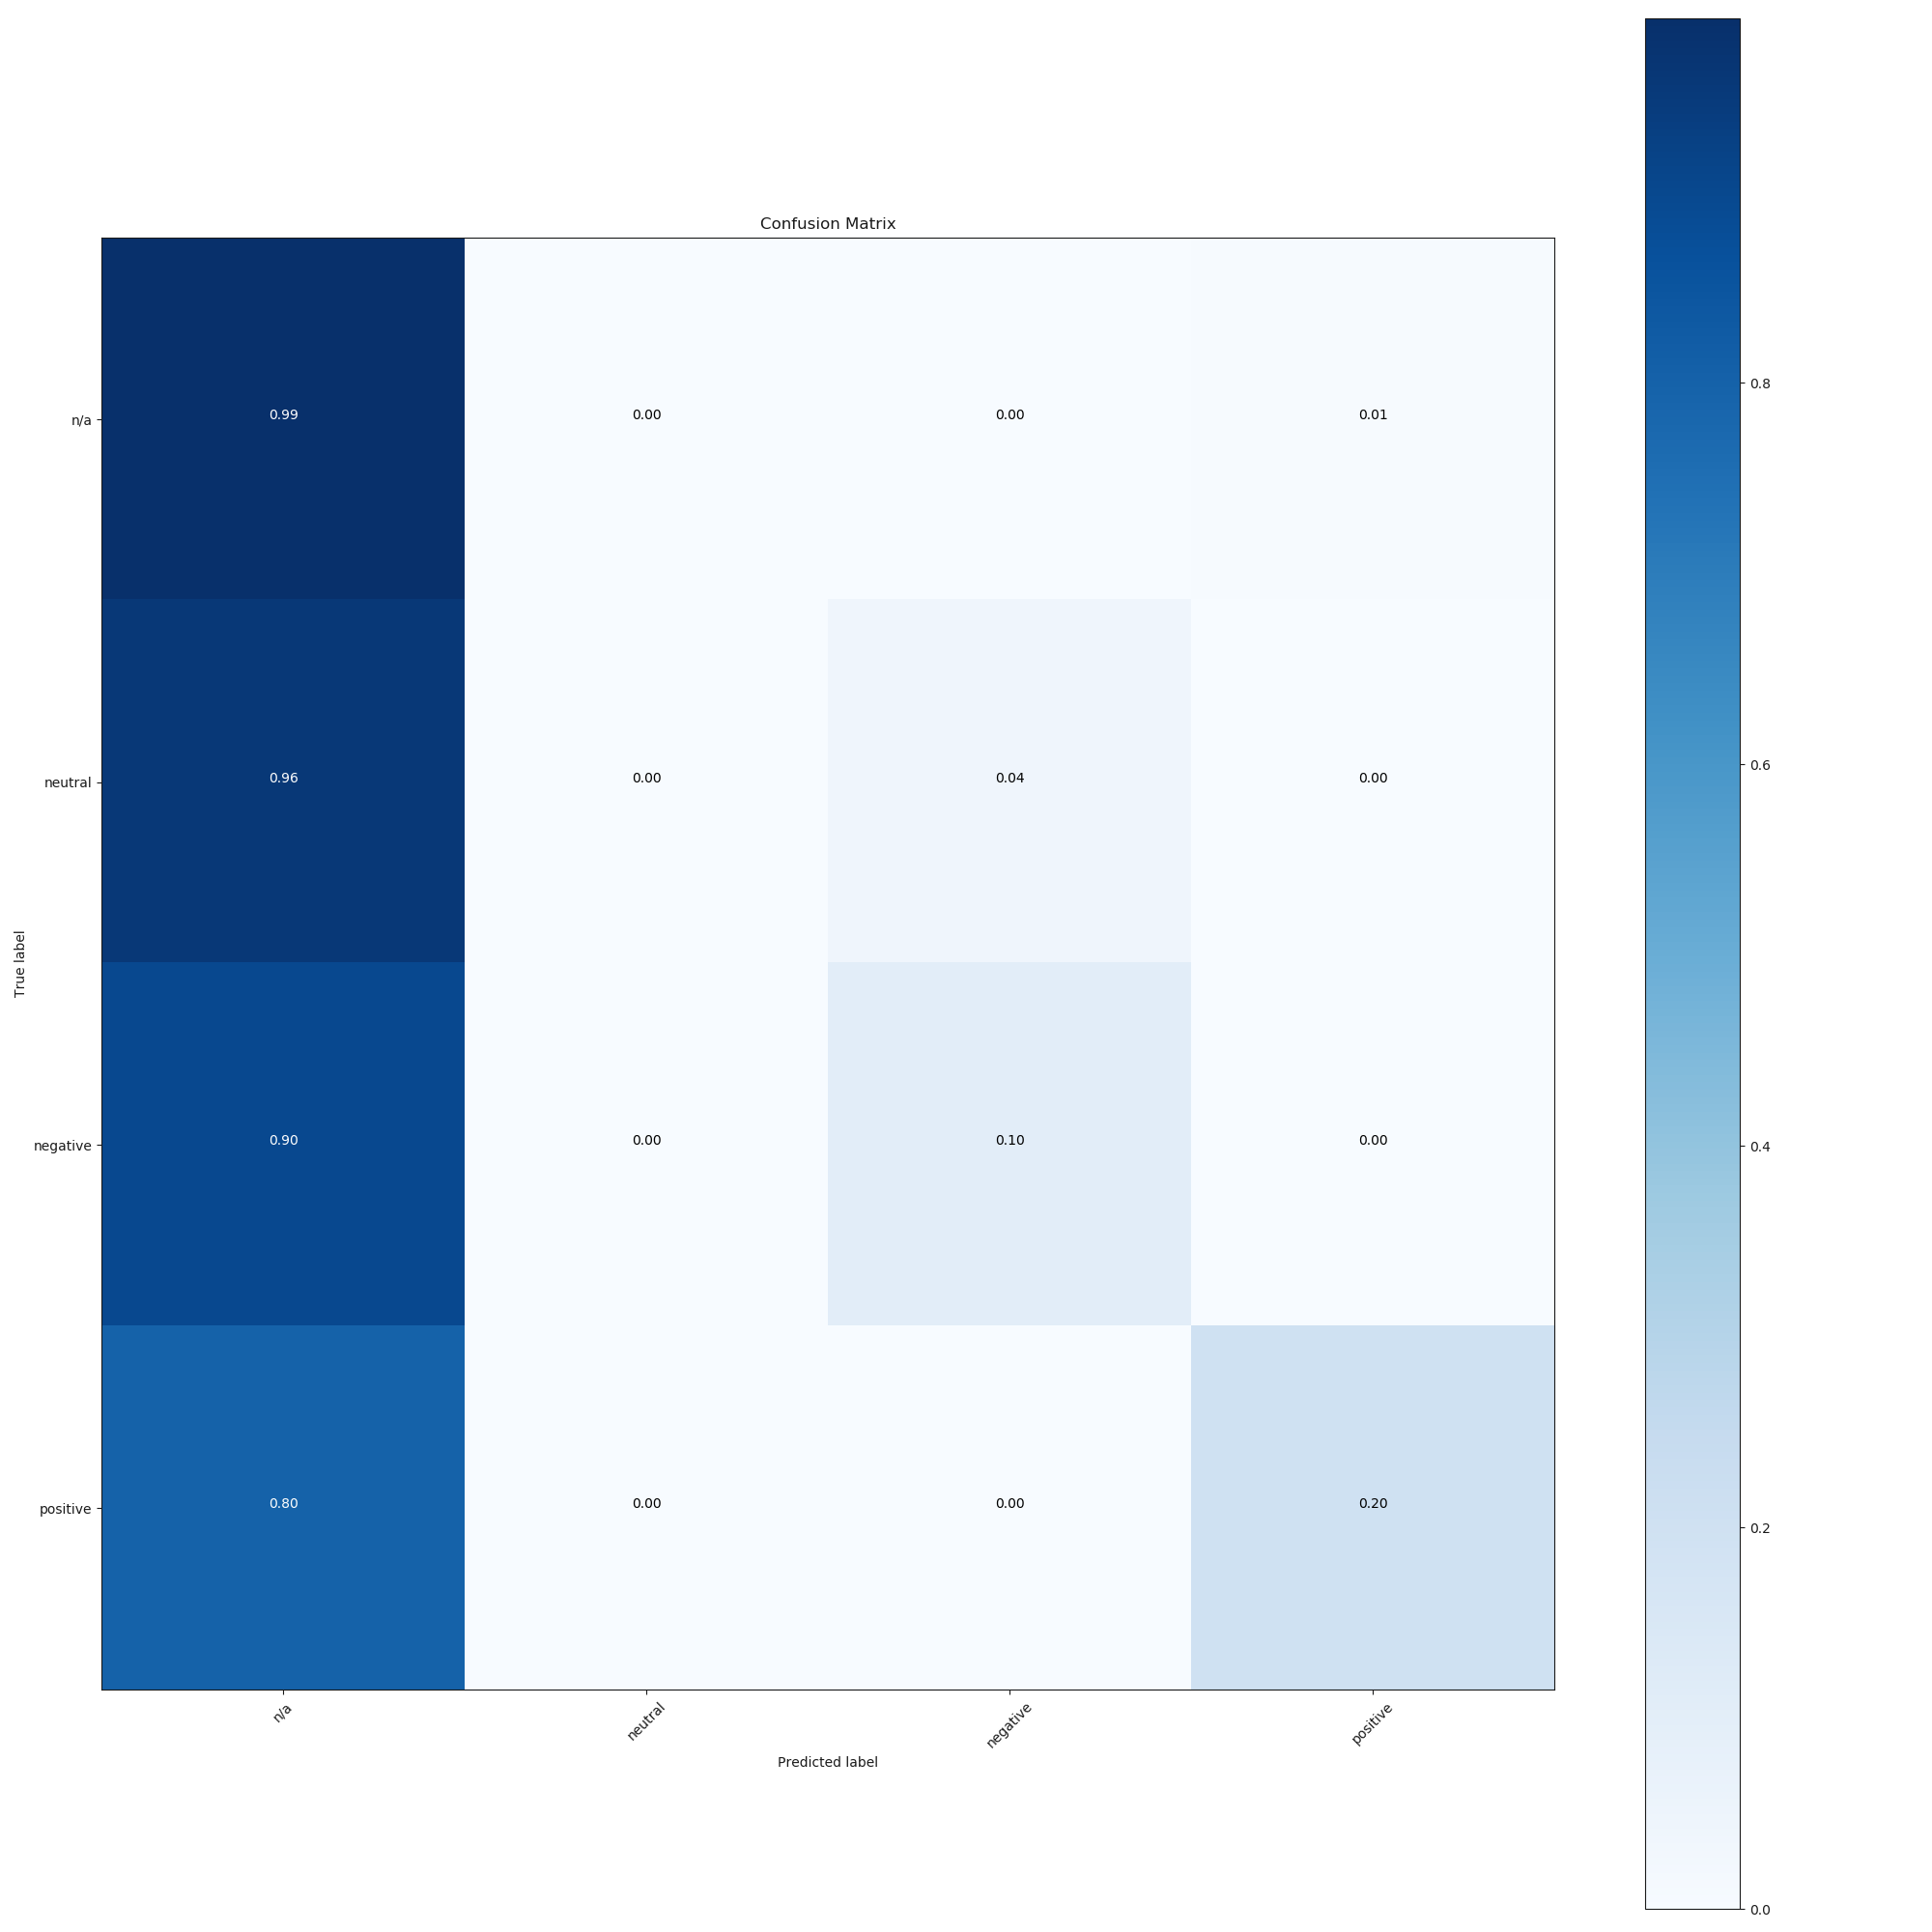
\includegraphics[width=0.19\textwidth]{figures/08_appendix/germeval/08_11}
    }
    \subfloat[Komfort]{
        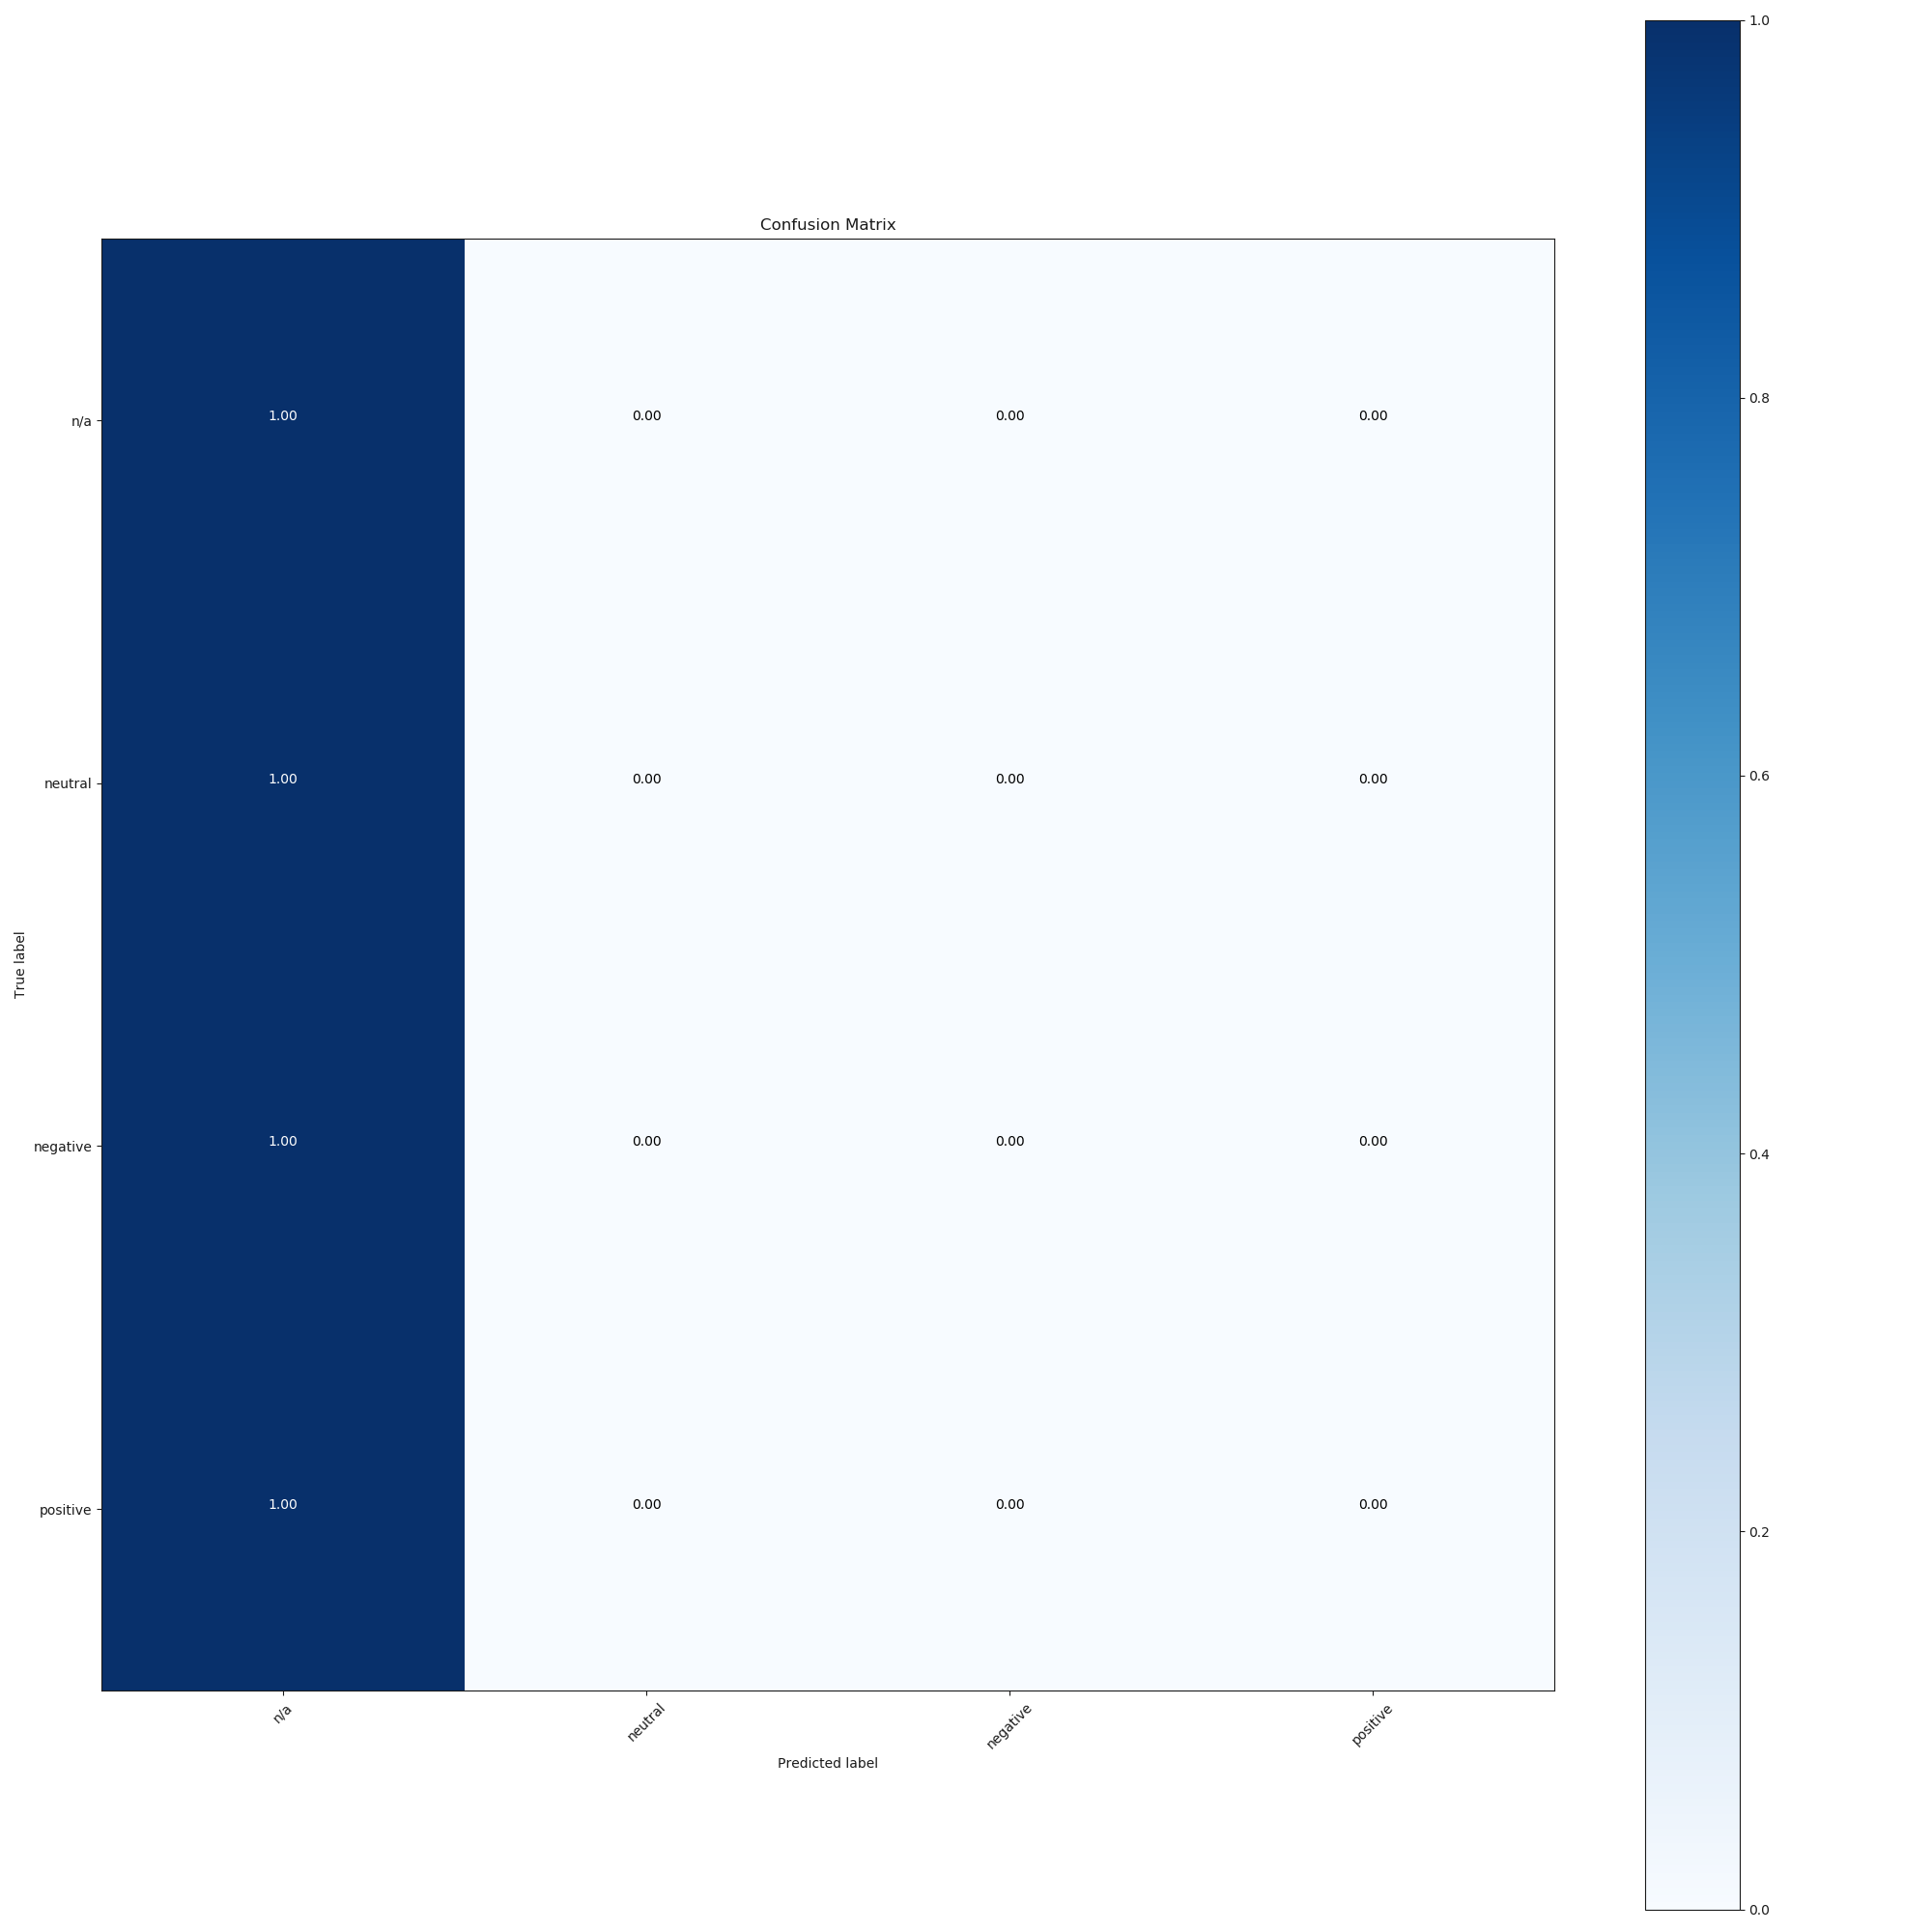
\includegraphics[width=0.19\textwidth]{figures/08_appendix/germeval/08_12}
    }
    \subfloat[QR-Code]{
        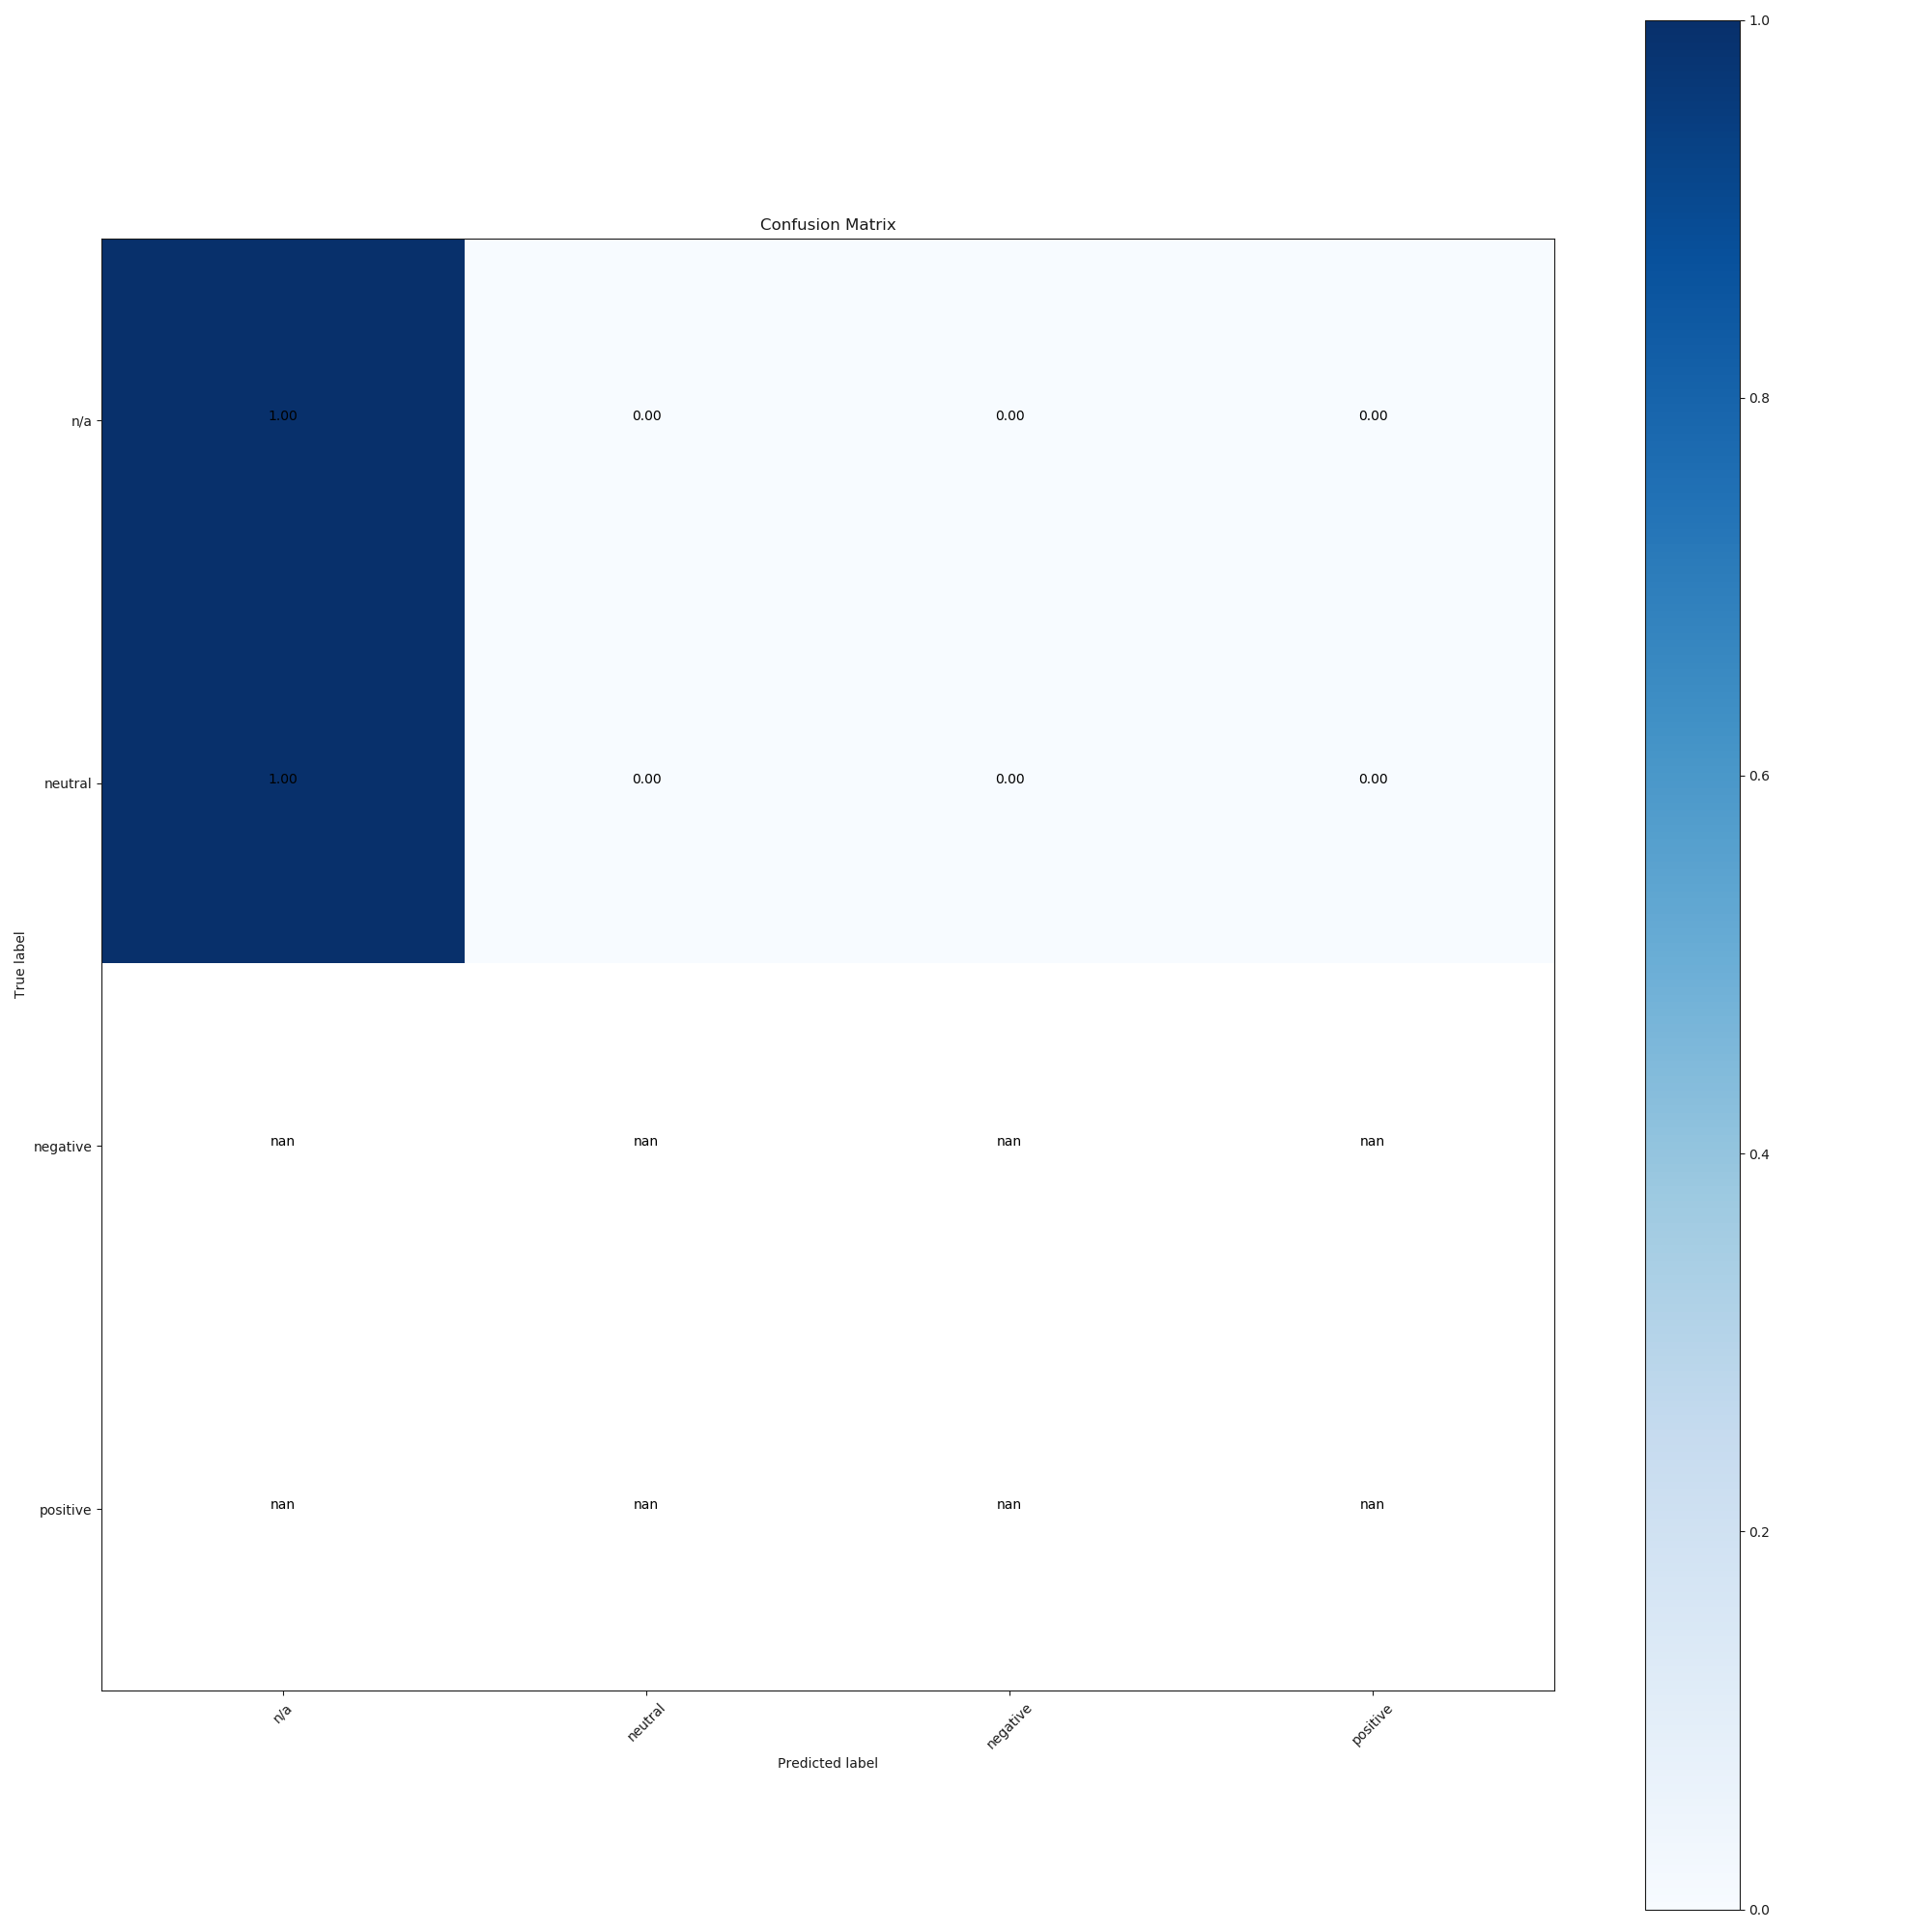
\includegraphics[width=0.19\textwidth]{figures/08_appendix/germeval/08_13}
    }
    \subfloat[Reise m. Kindern]{
        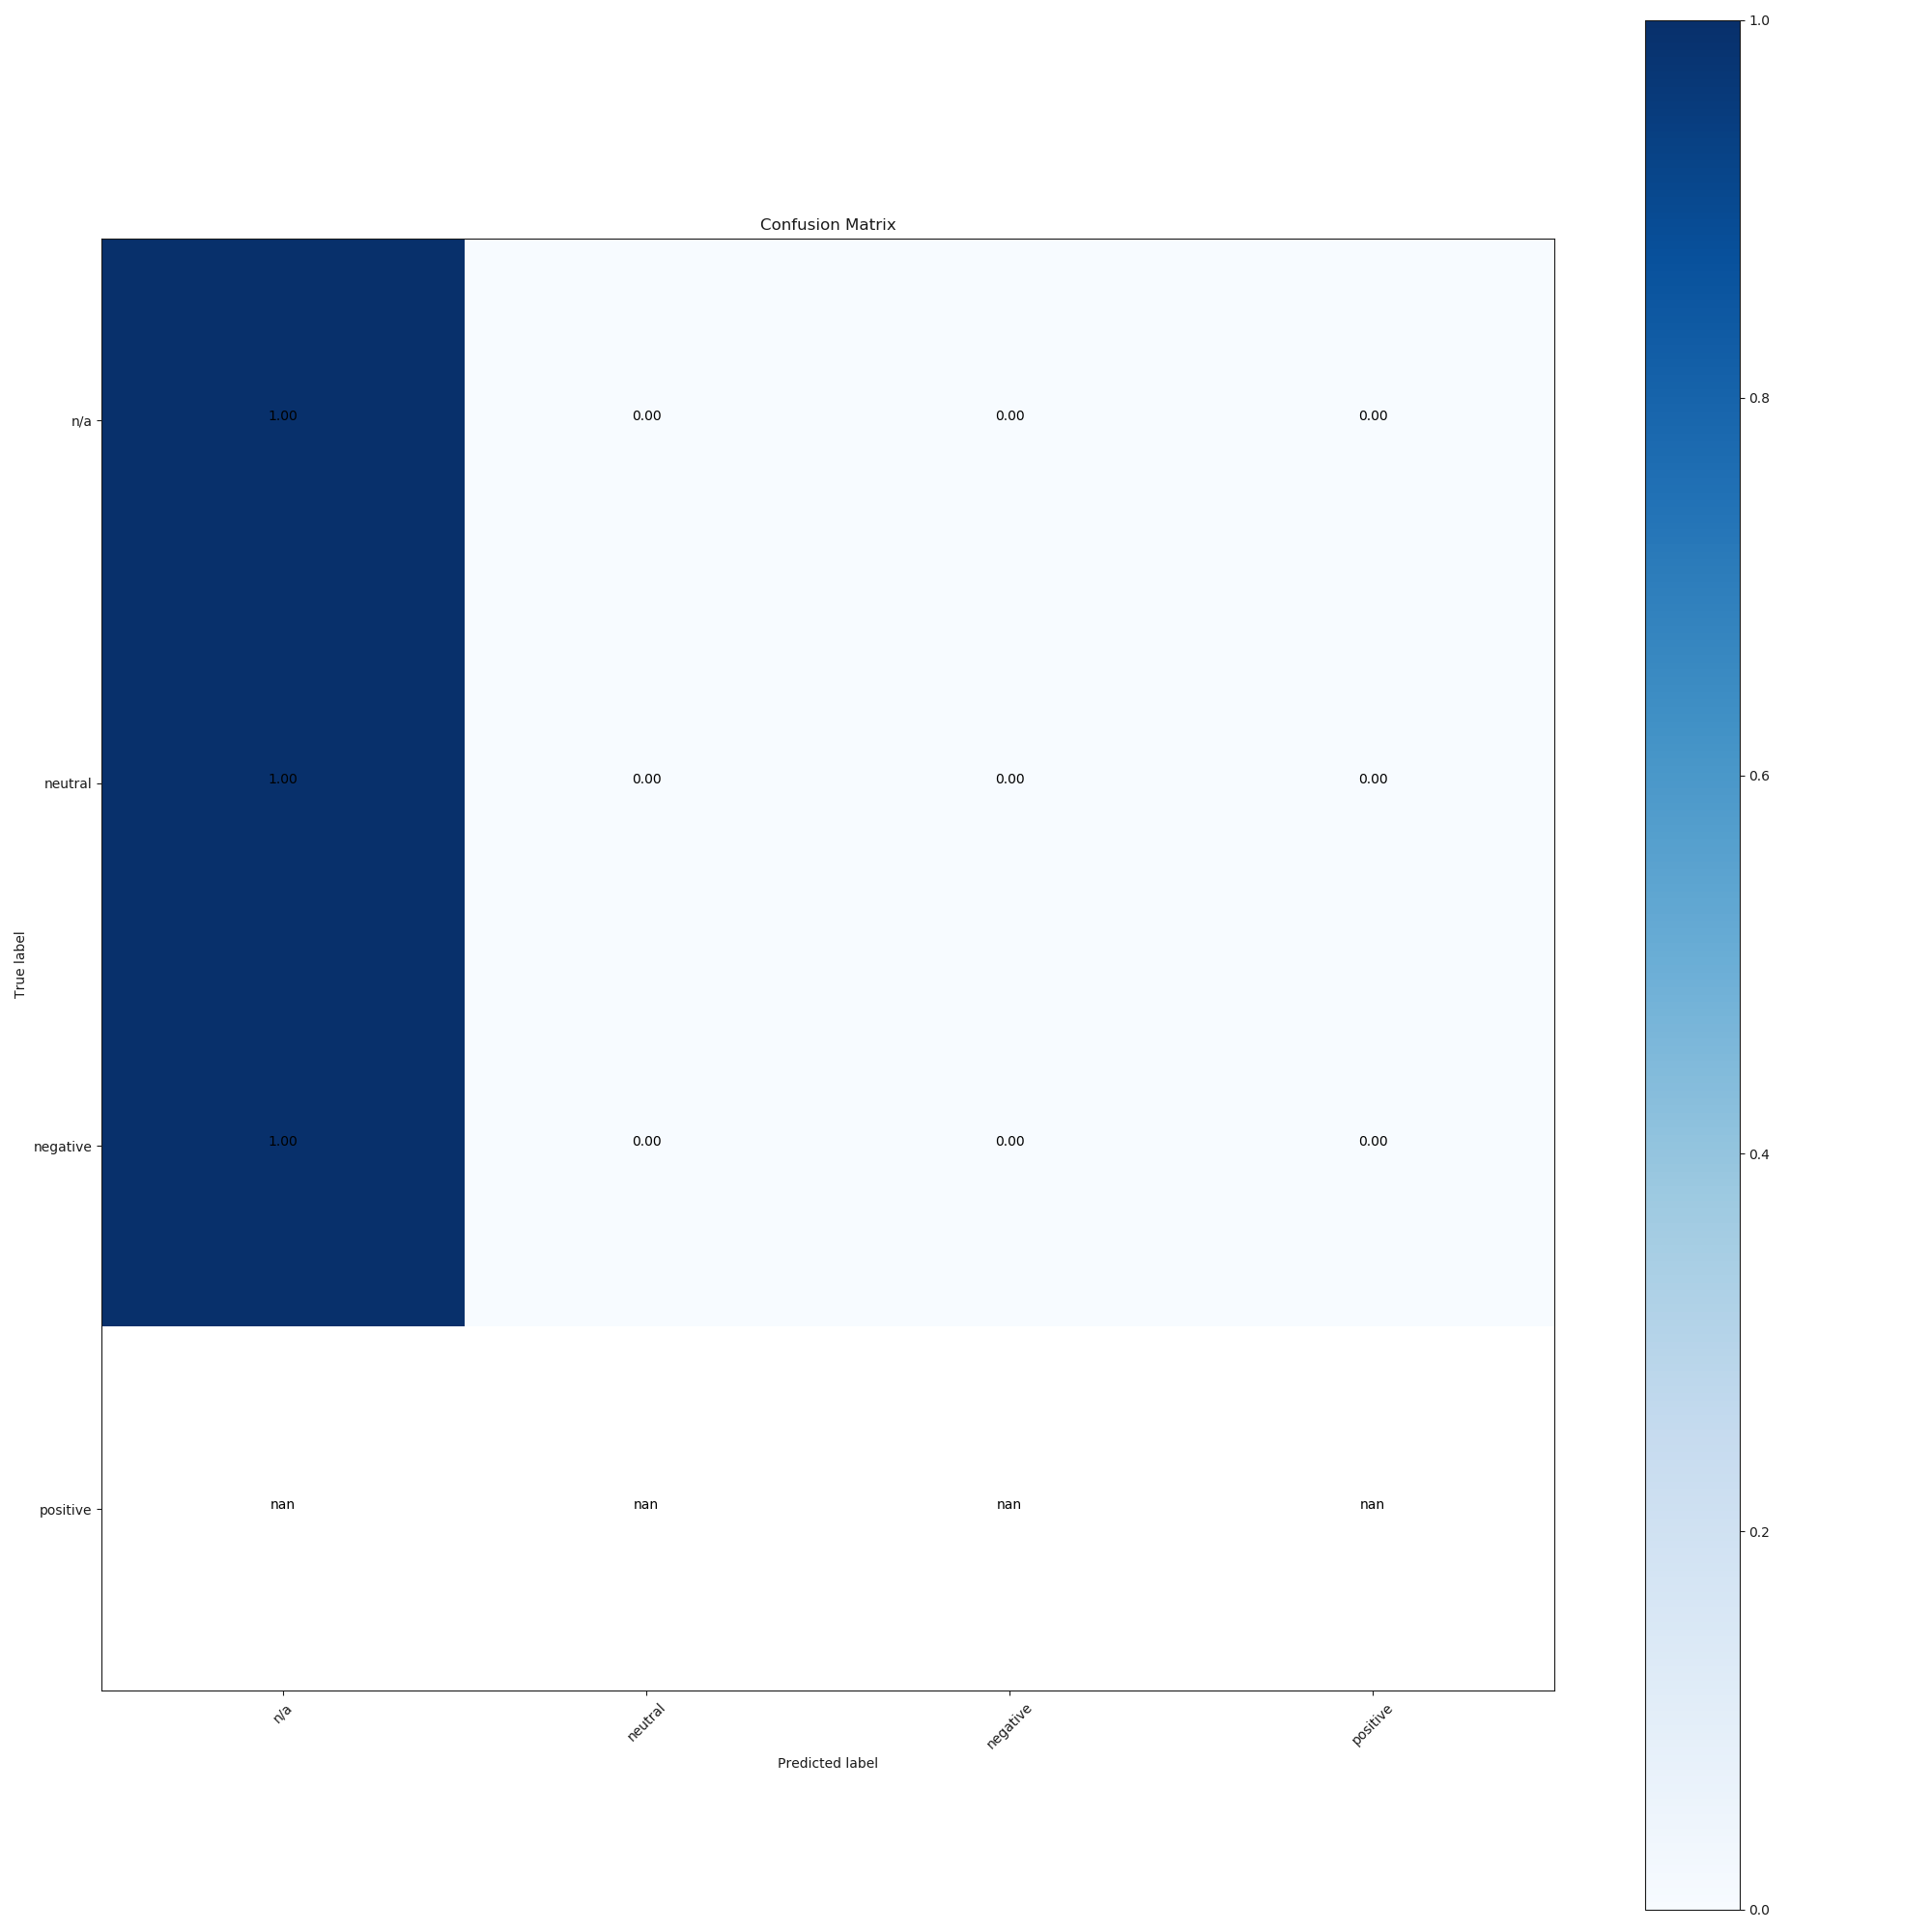
\includegraphics[width=0.19\textwidth]{figures/08_appendix/germeval/08_14}
    }
    \subfloat[Service \& Support]{
        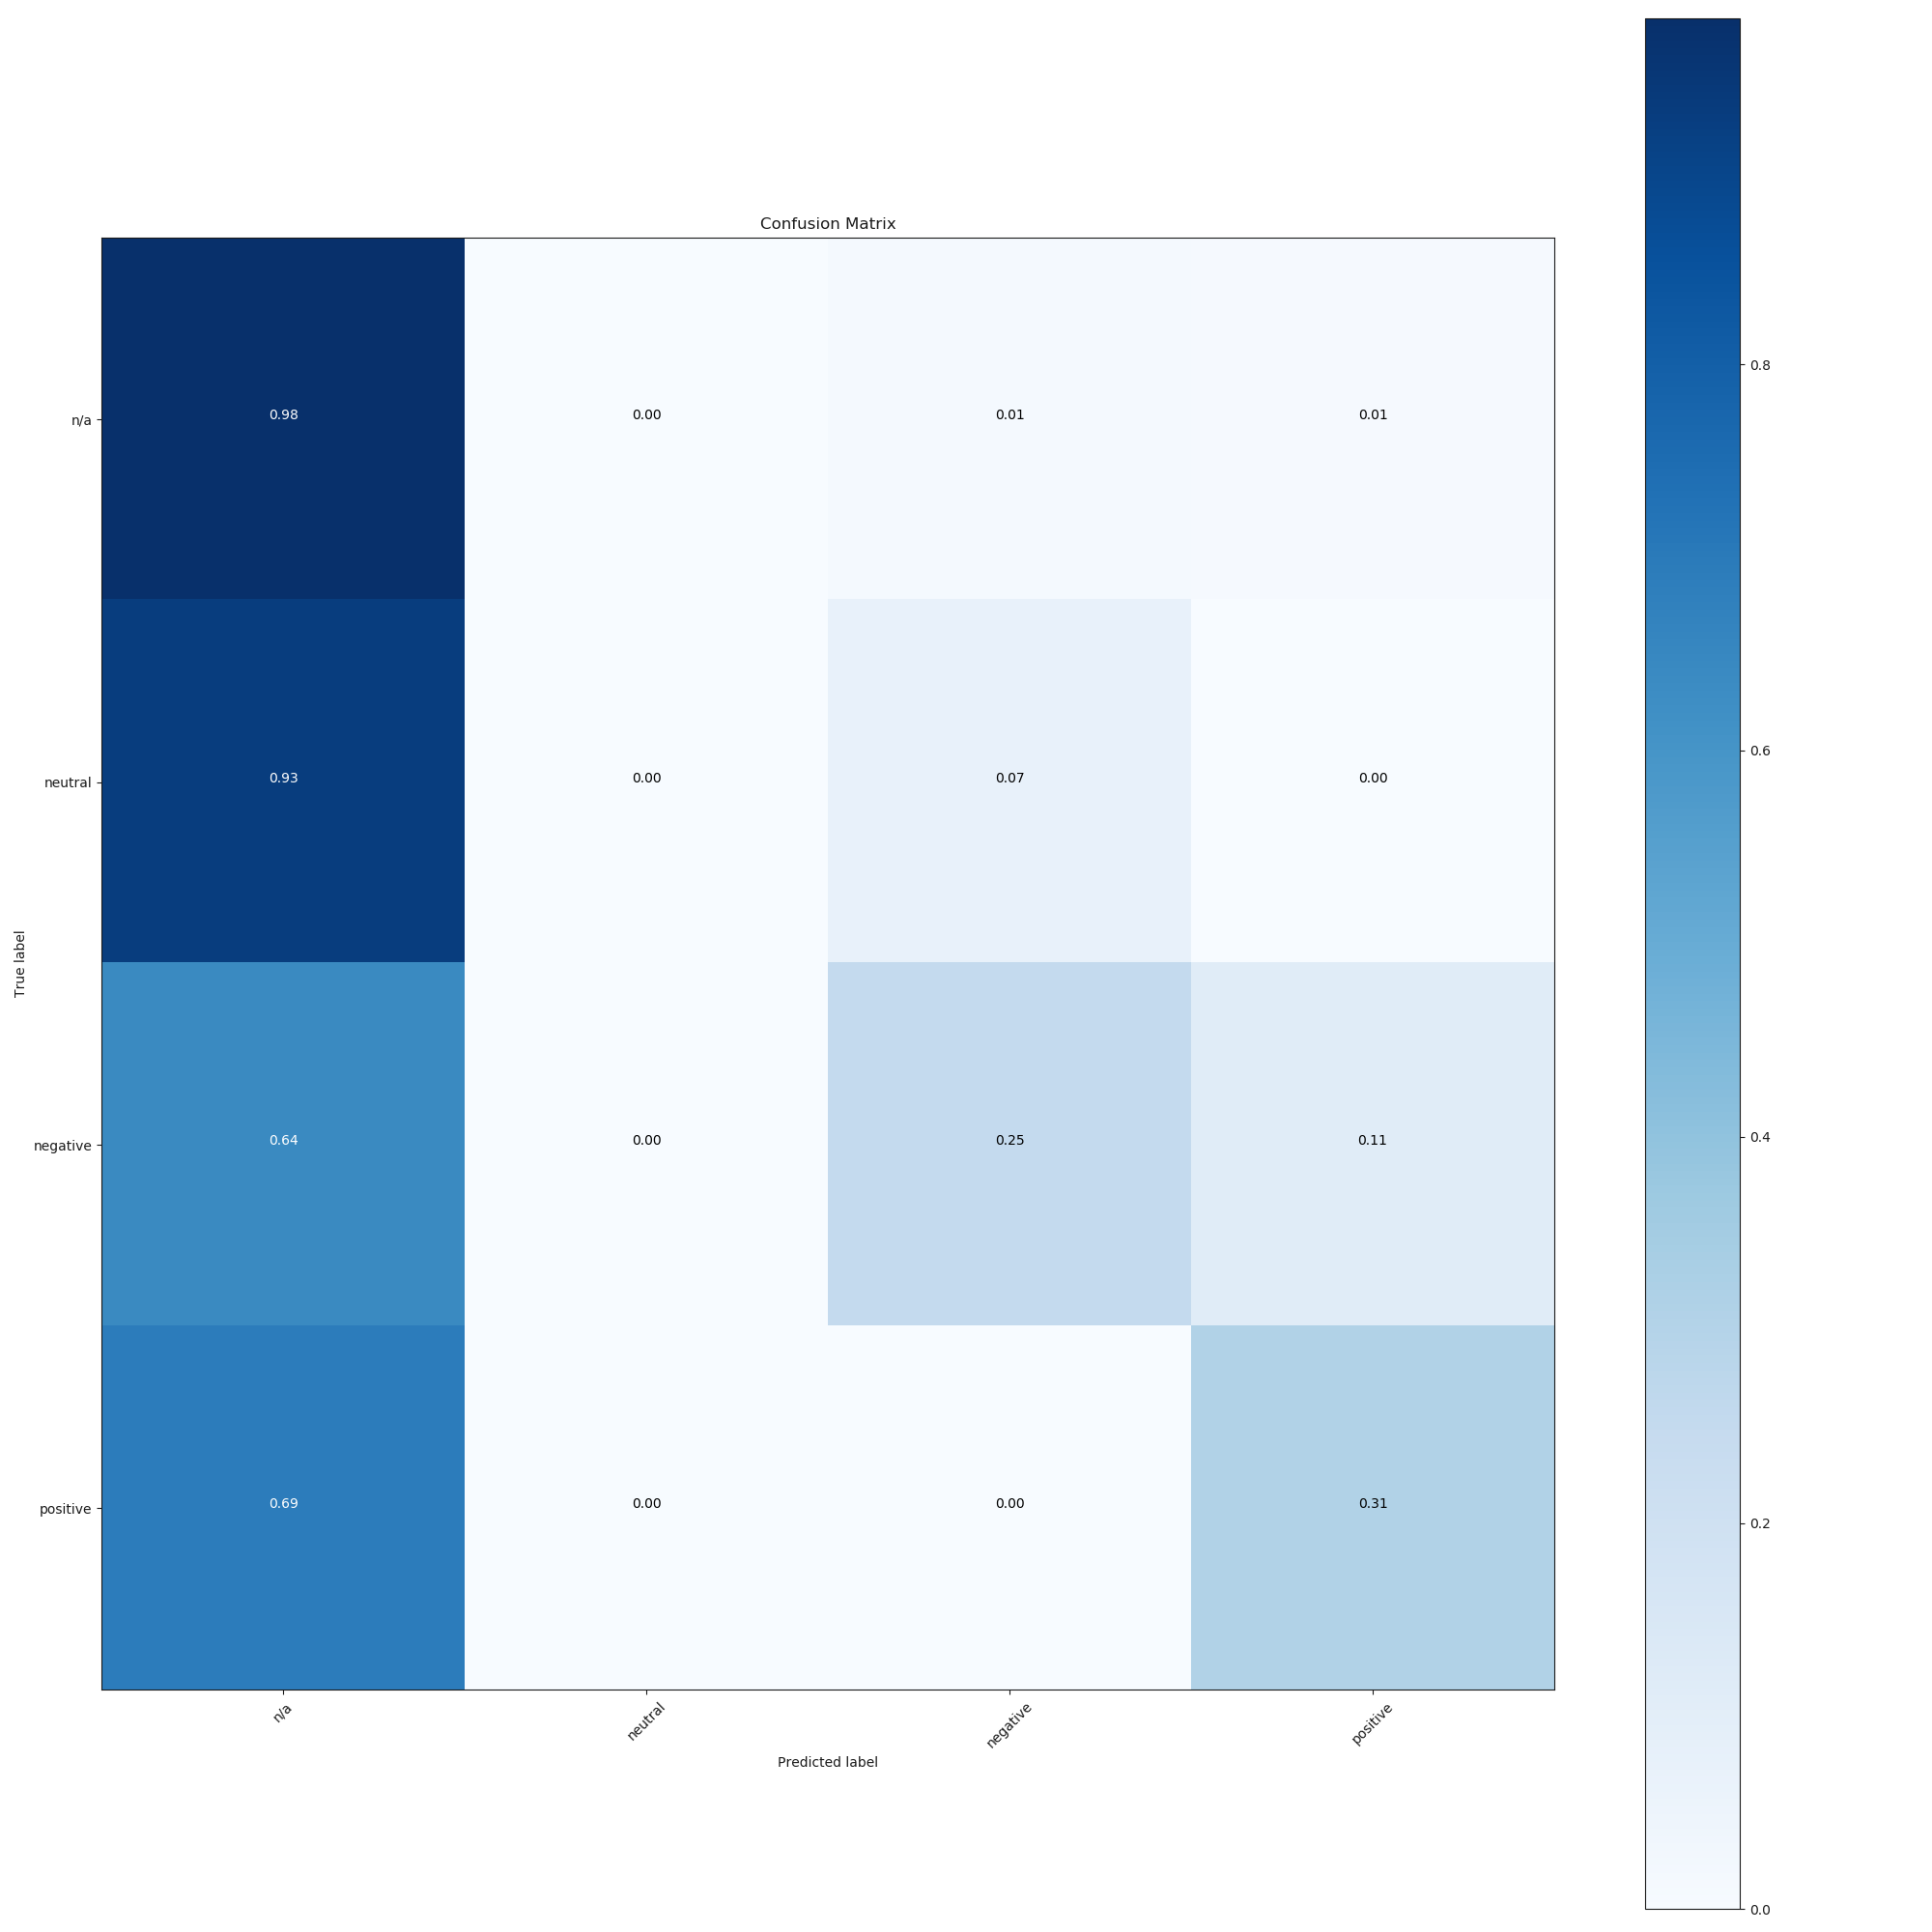
\includegraphics[width=0.19\textwidth]{figures/08_appendix/germeval/08_15}
    }
    \hspace{0mm}

    \subfloat[Sicherheit]{
        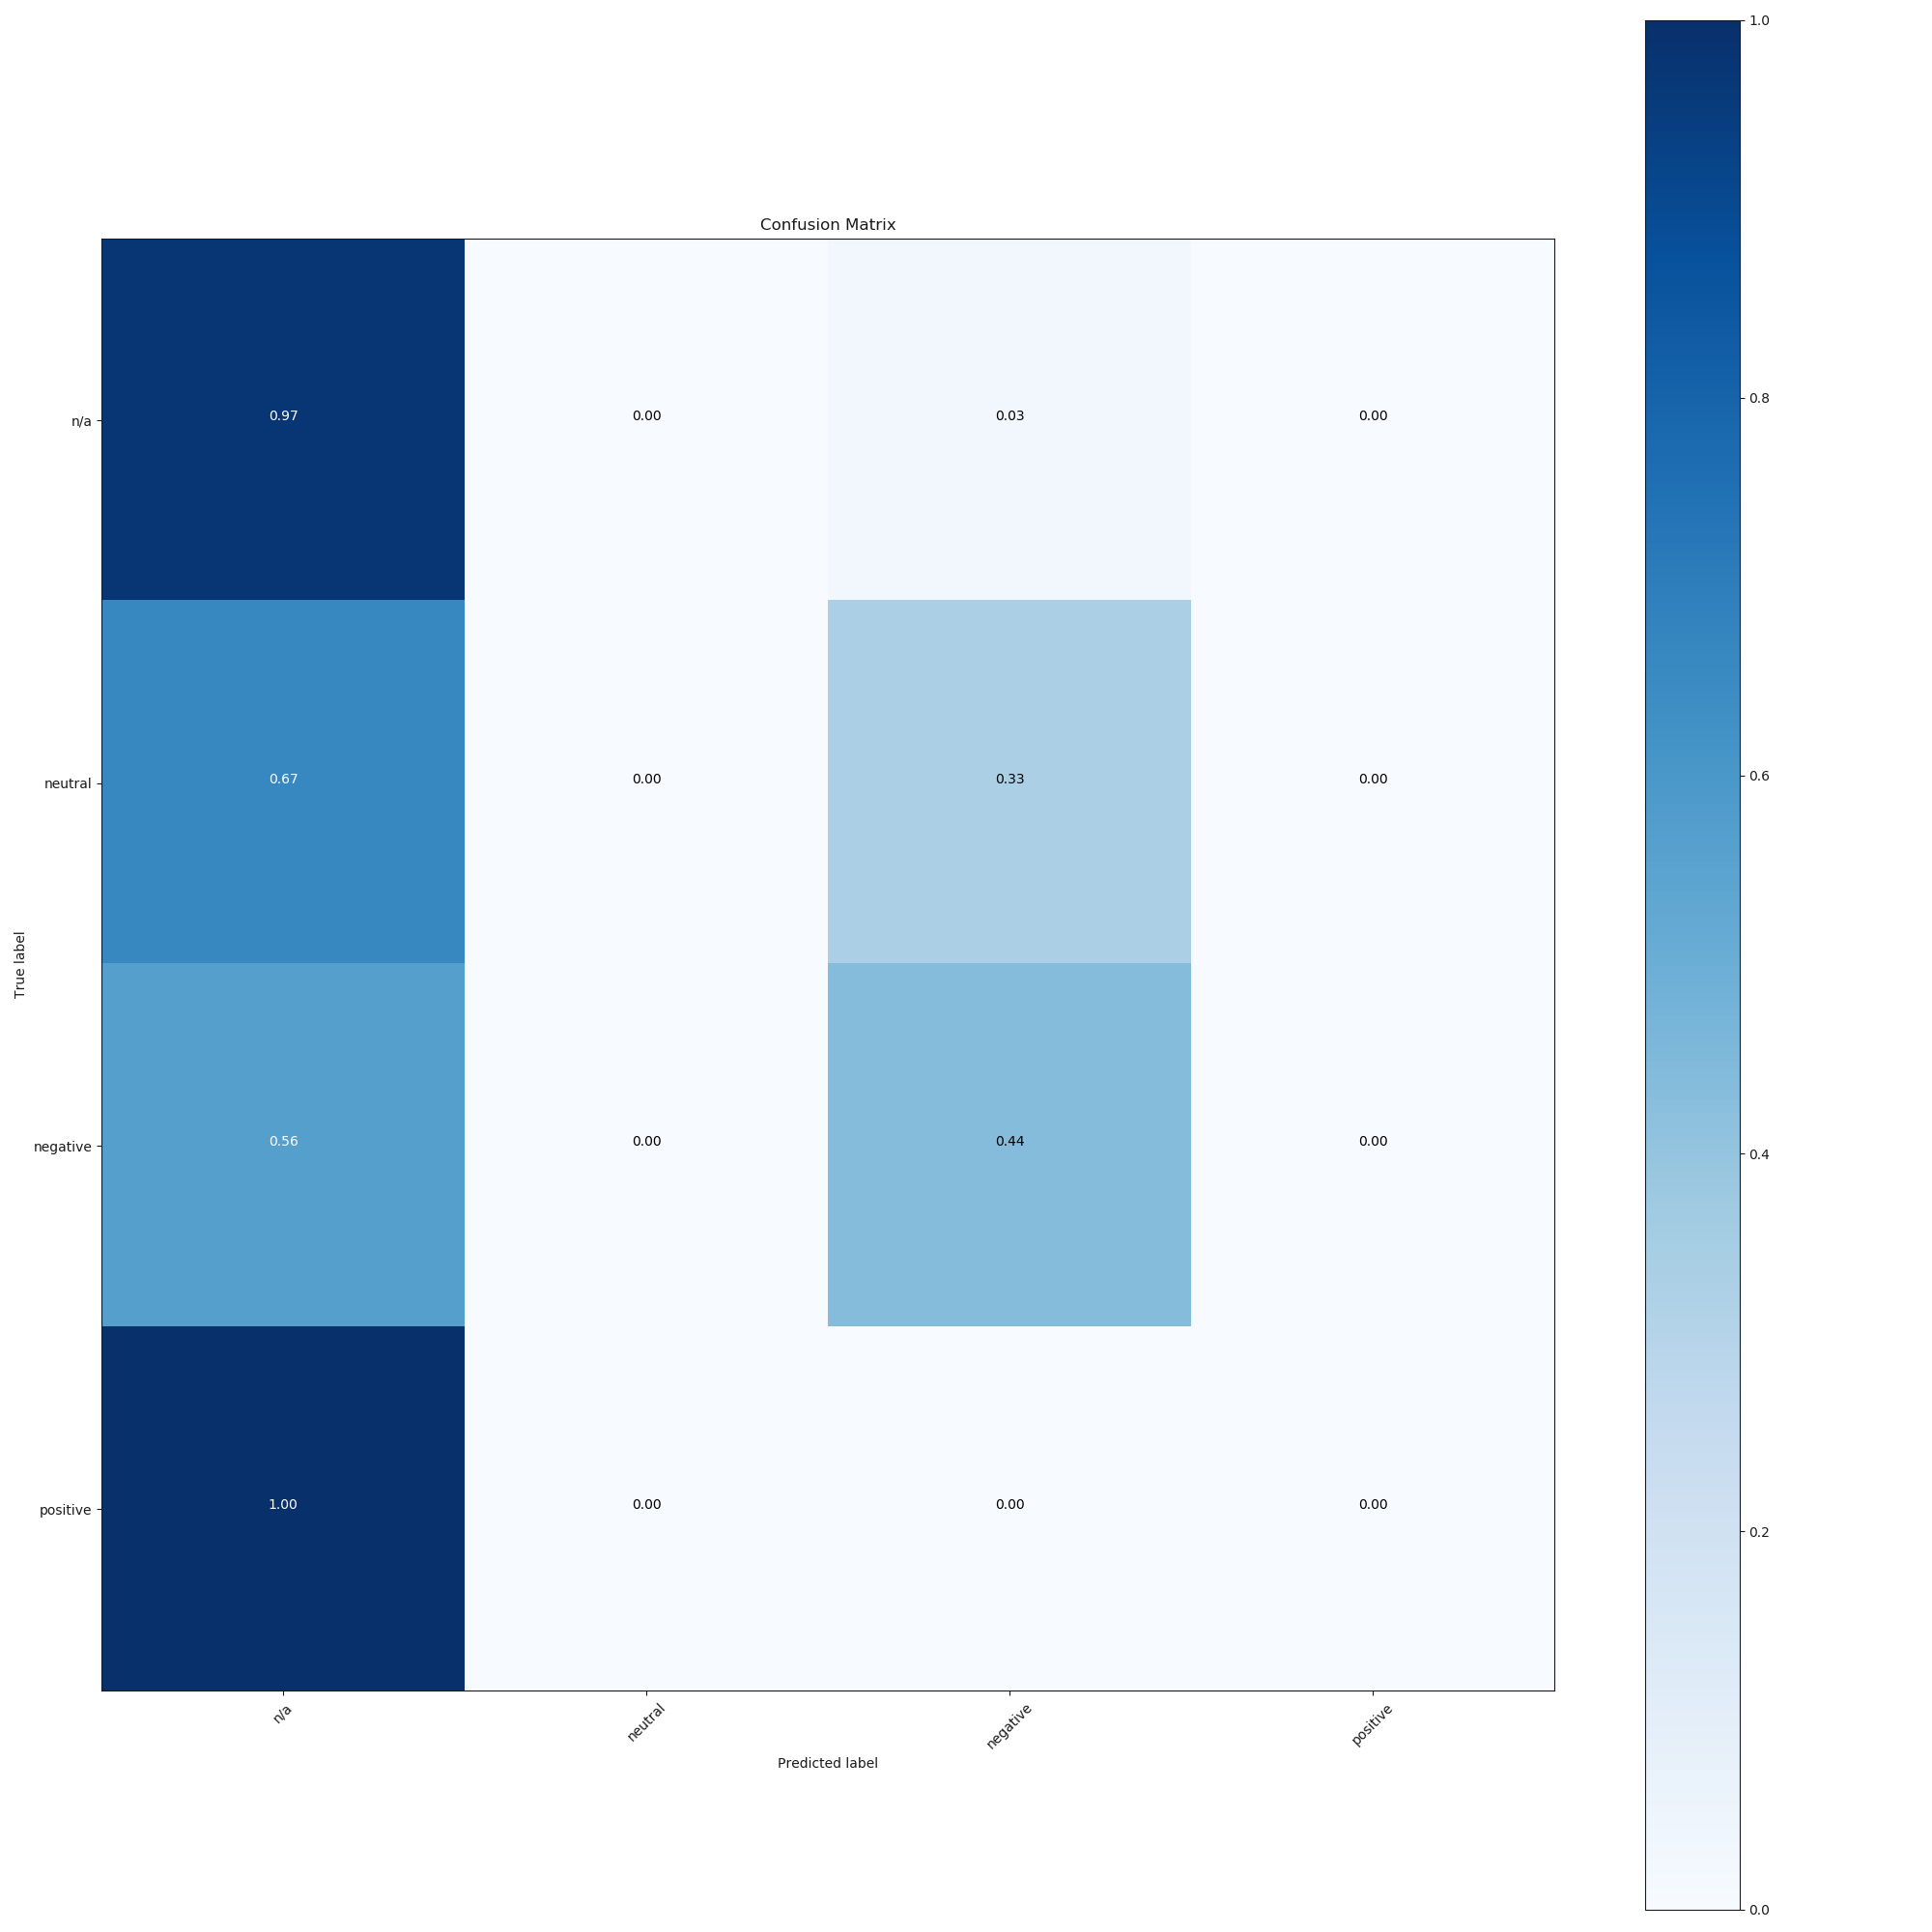
\includegraphics[width=0.19\textwidth]{figures/08_appendix/germeval/08_16}
    }
    \subfloat[Unregelmäßigkeiten]{
        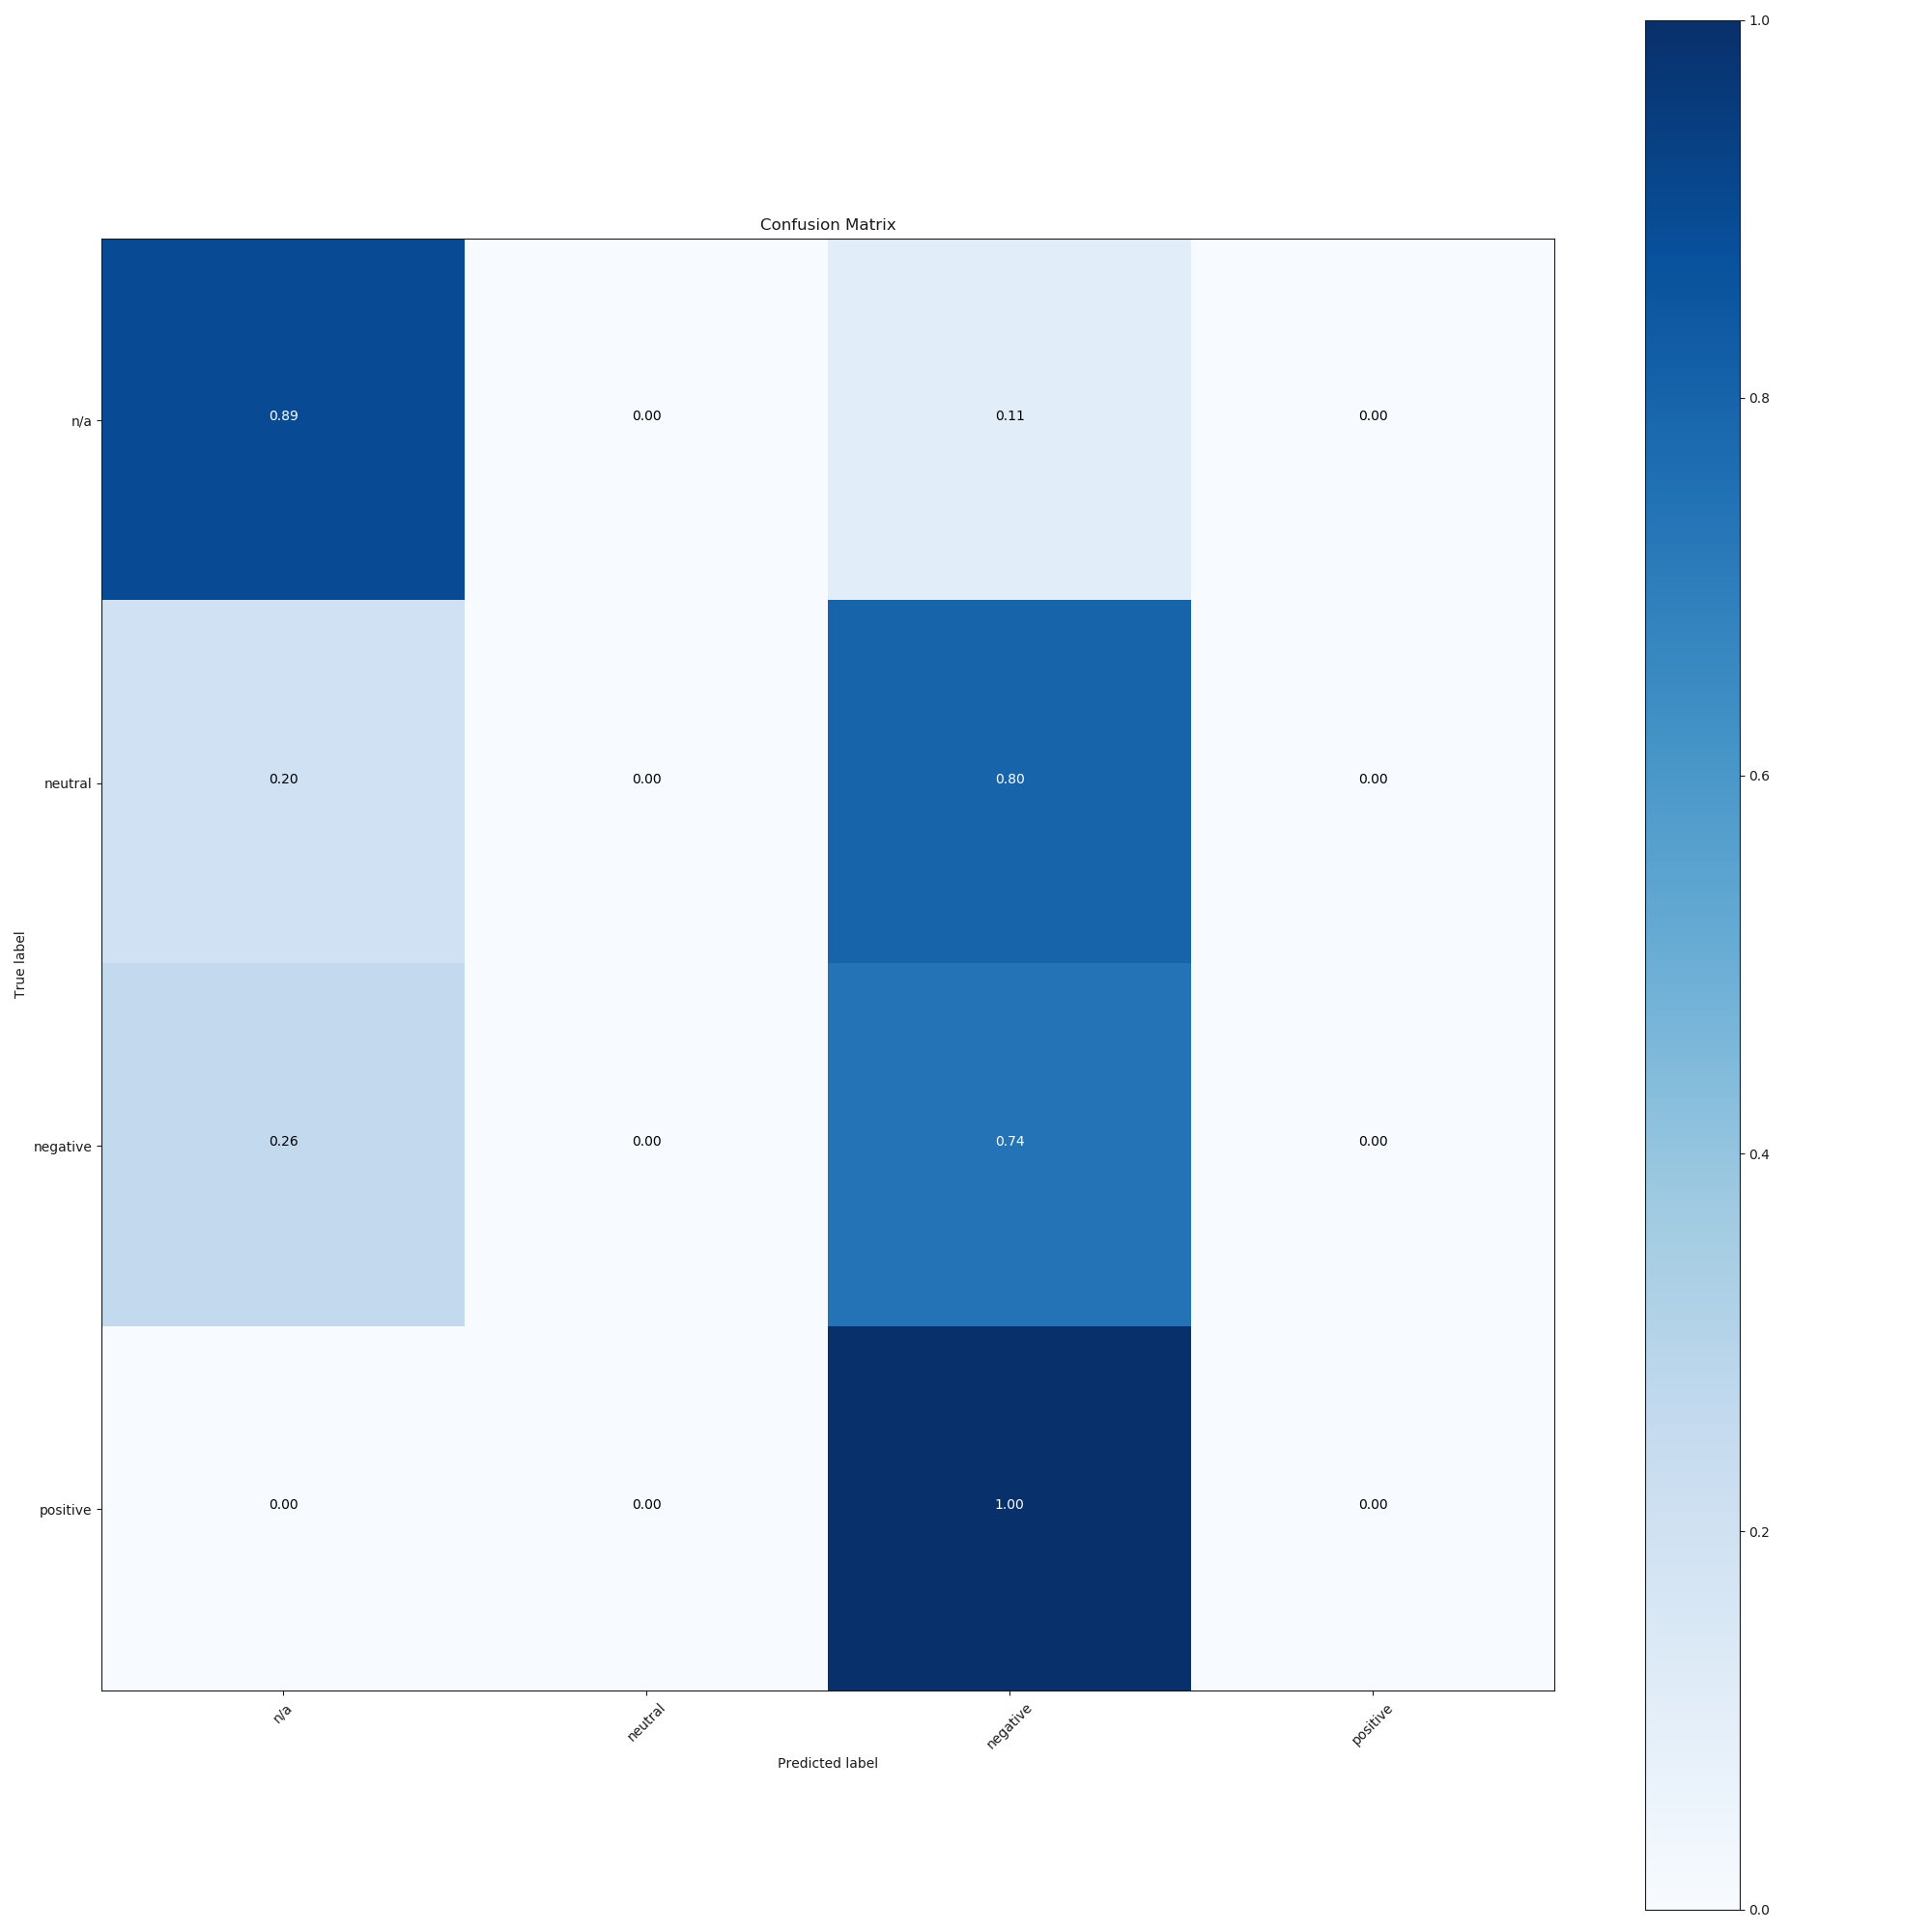
\includegraphics[width=0.19\textwidth]{figures/08_appendix/germeval/08_17}
    }
    \subfloat[Ticketkauf]{
        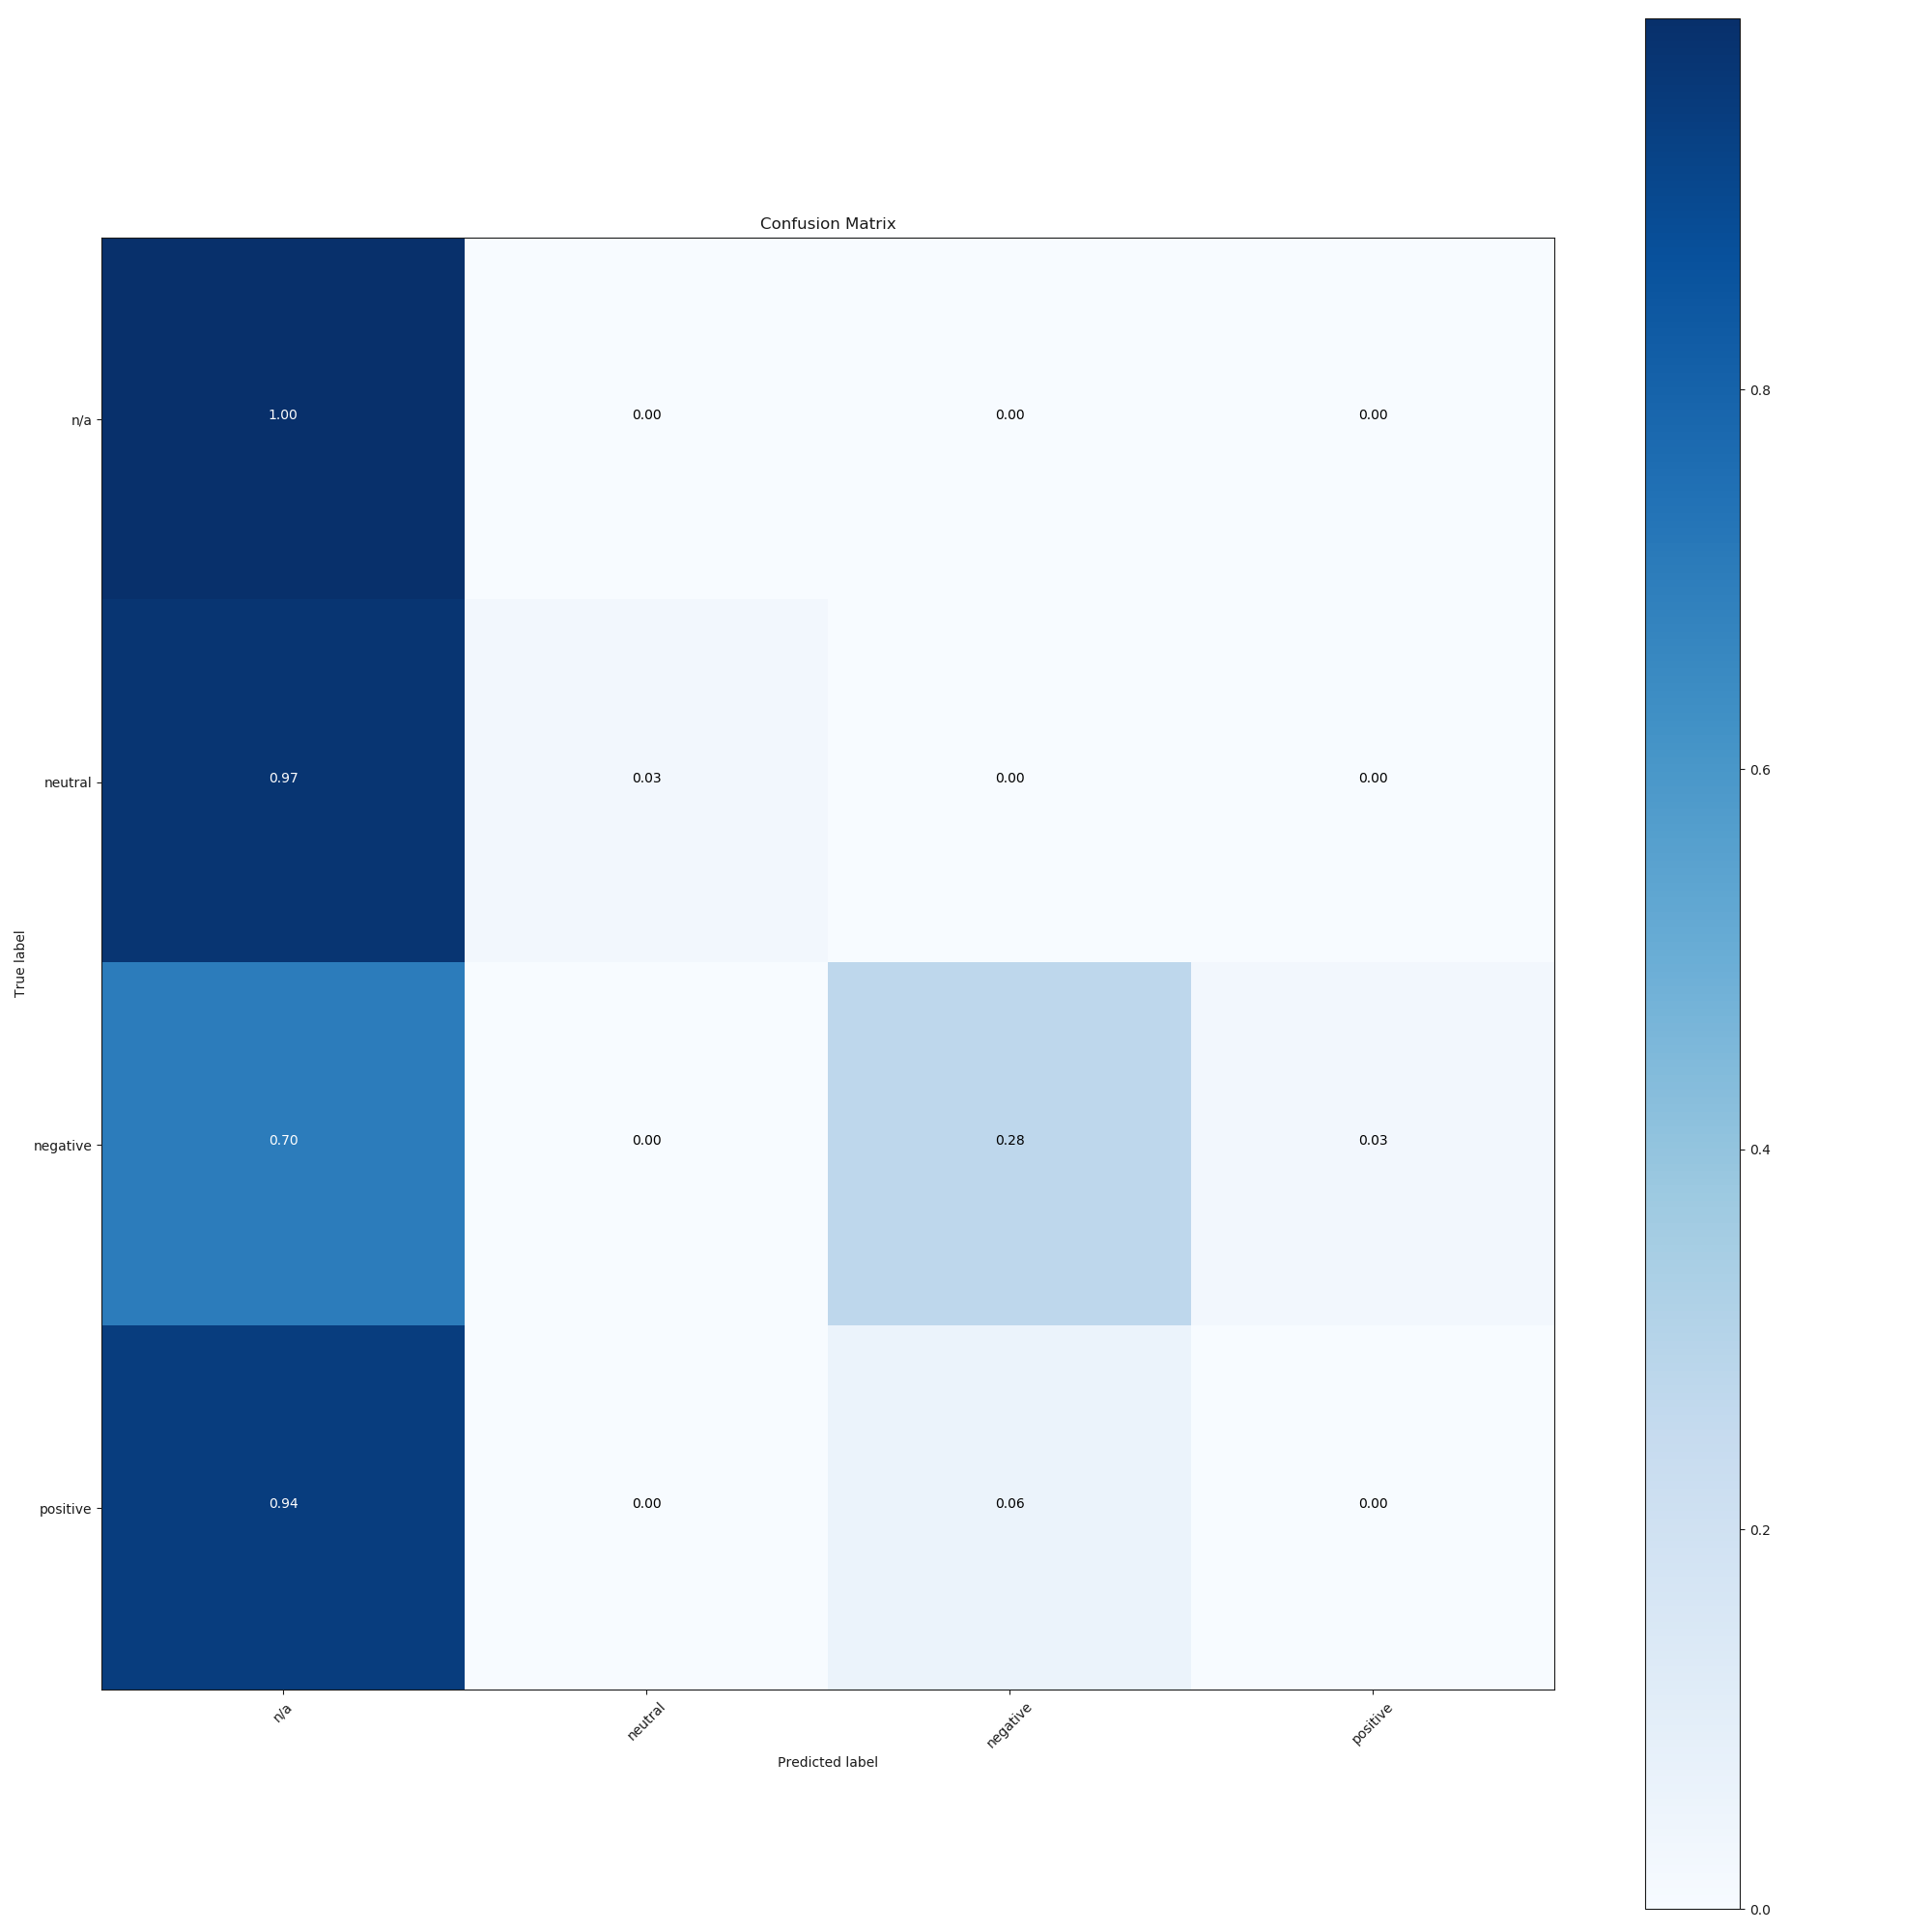
\includegraphics[width=0.19\textwidth]{figures/08_appendix/germeval/08_18}
    }
    \subfloat[Toiletten]{
        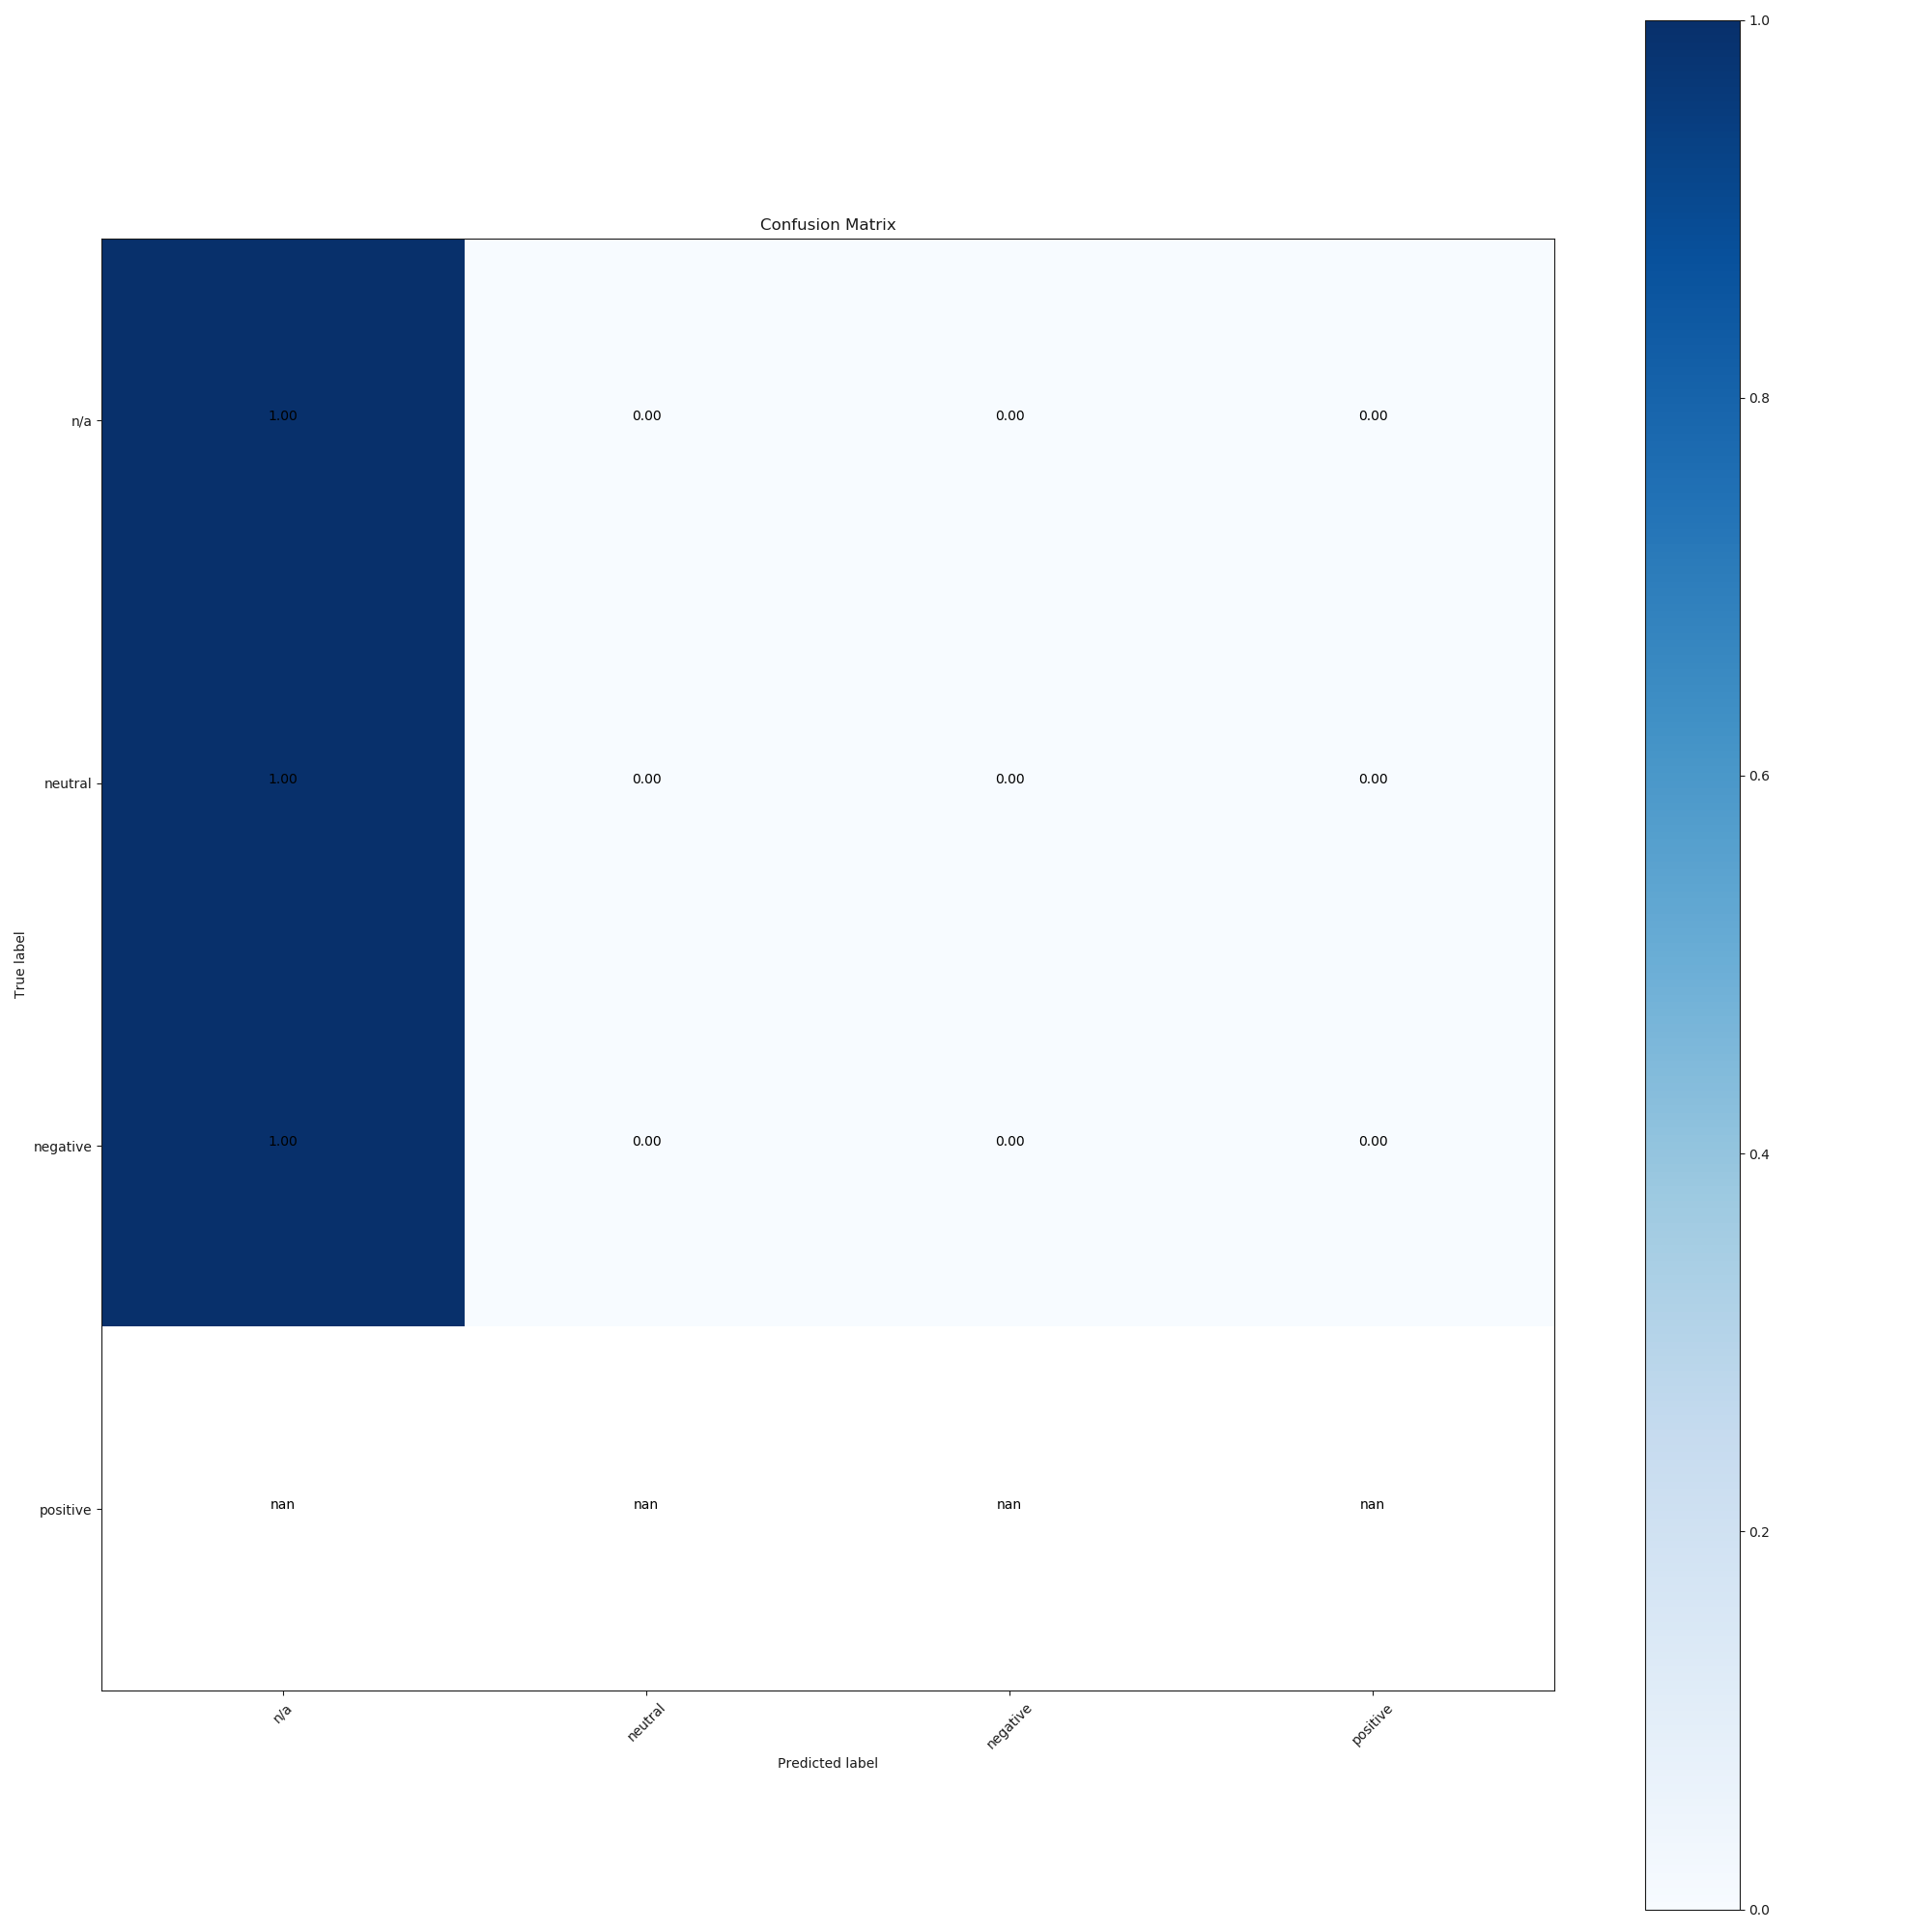
\includegraphics[width=0.19\textwidth]{figures/08_appendix/germeval/08_19}
    }
    \subfloat[Zugfahrt]{
        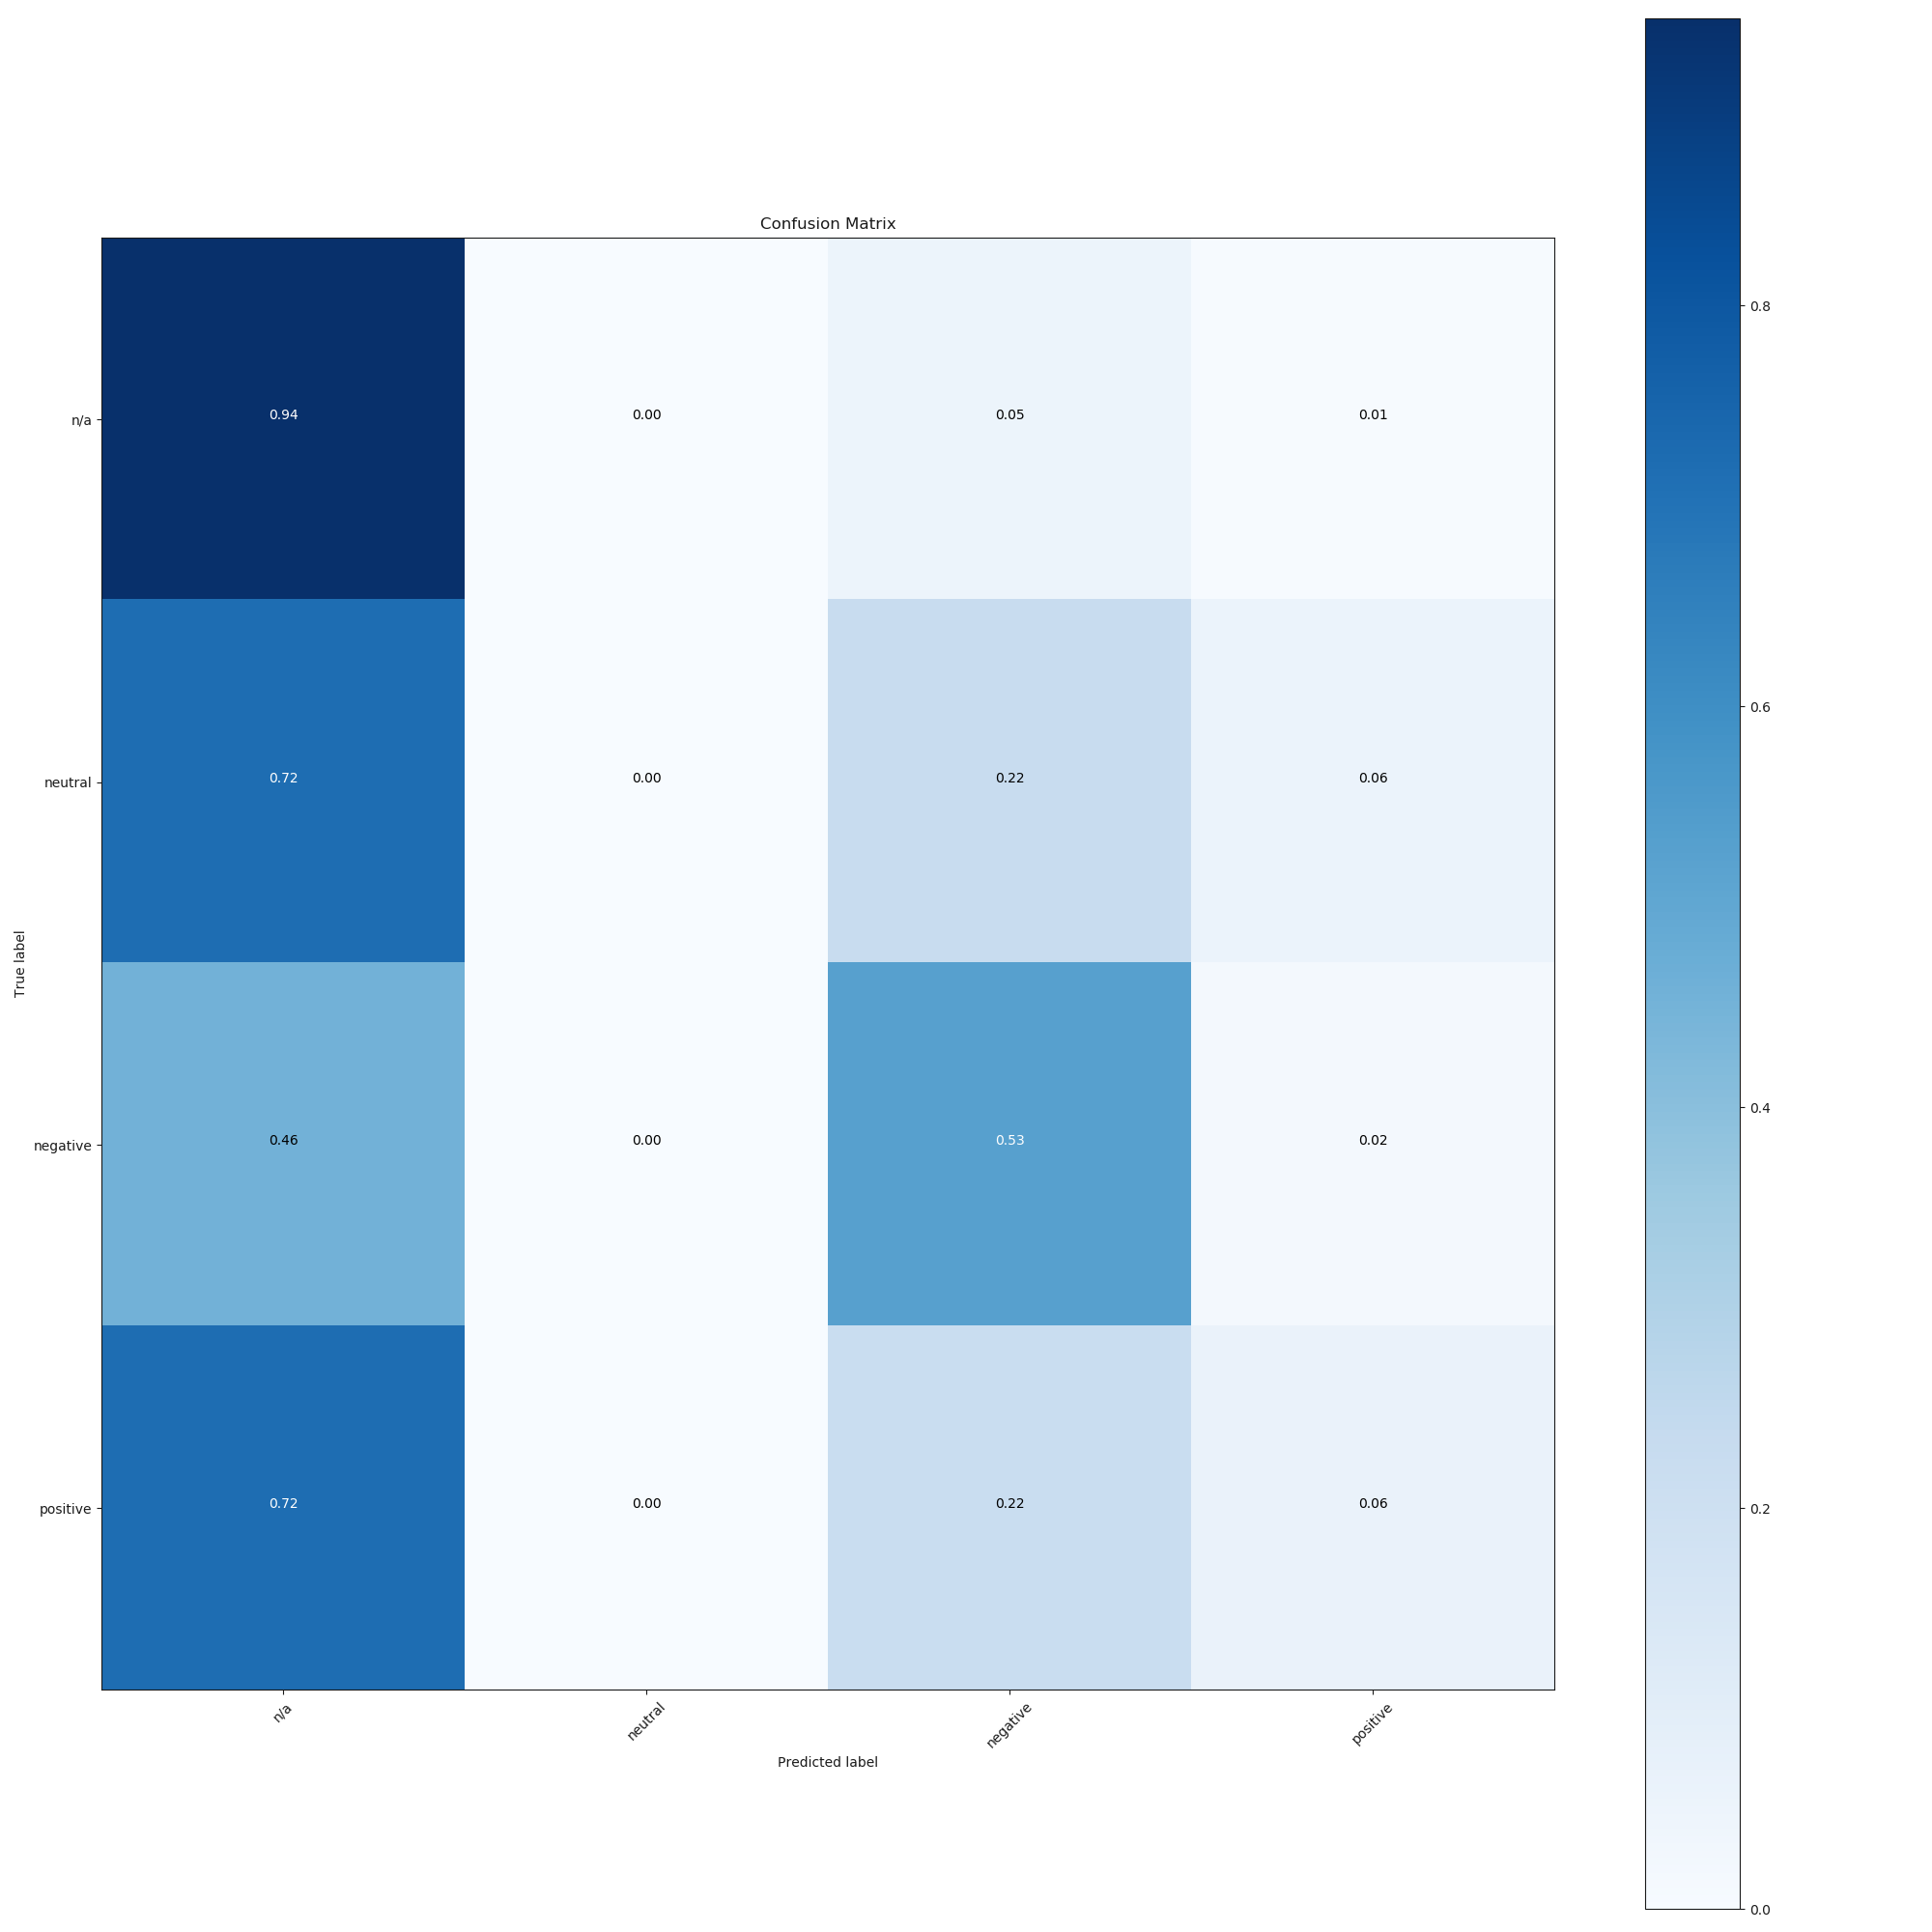
\includegraphics[width=0.19\textwidth]{figures/08_appendix/germeval/08_20}
    }    \hspace{0mm}

\caption{\textbf{GermEval-2017 -- Confusion matrices of the aspect on the test split.} The figure shows a normalized confusion matrix for each aspect head. From left to right: n/a, neutral, positive, negative.}
\label{fig:08_ge_conf}
\end{figure}

\subsection{Amazon reviews}

\begin{figure}[H]
    \centering
    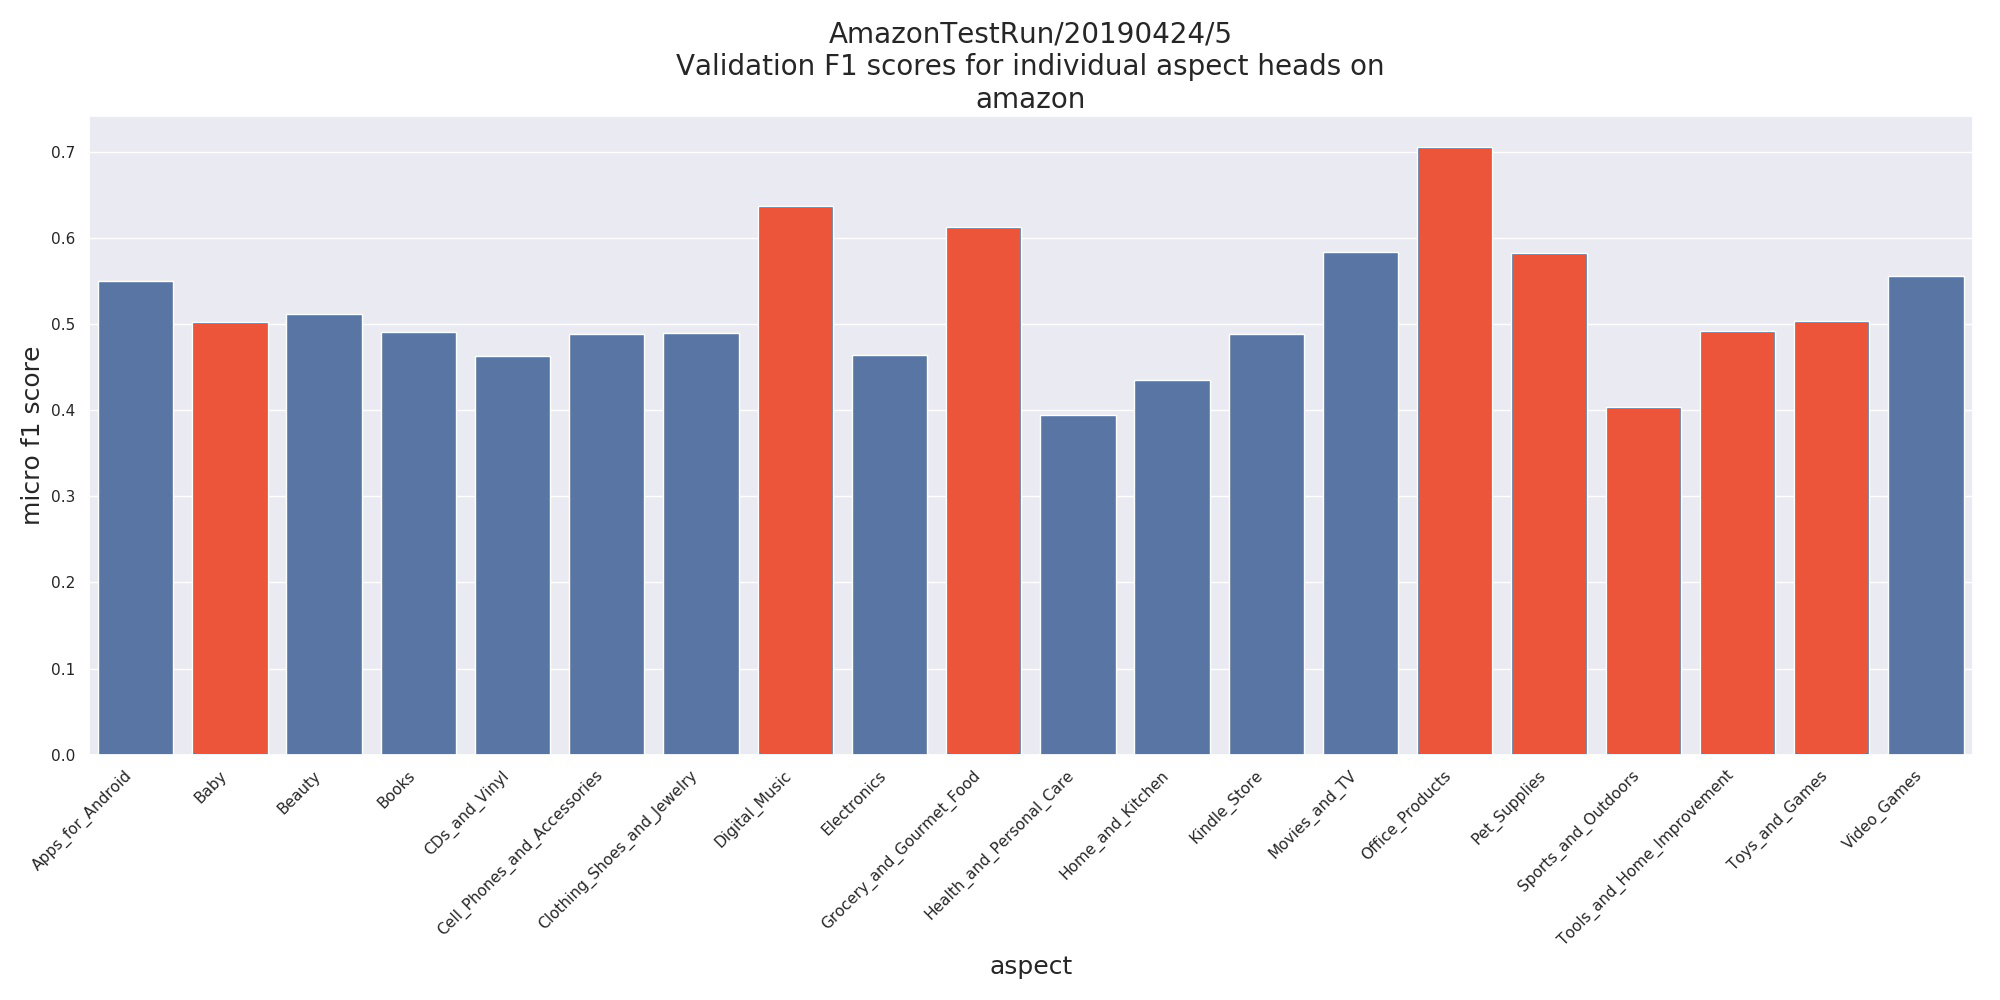
\includegraphics[width=\textwidth]{figures/08_appendix/08_am_headResults}
    \caption{\textbf{Amazon Reviews -- Micro F1 scores}. Individual aspect head micro F1 scores achieved on the validation set of the custom Amazon reviews dataset. This figure reports the overall micro F1 score for the aspect heads without including the metrics for the n/a labels. The classes, marked as red which are not balanced along the sentiment dimension are Baby, Digital Music, Grocery \& Gourmet Food, Office Products, Pet Supplies, Sports and Outdoors, Tools and Home Improvement and Toys \& Games.}
    \label{fig:08_am_val_f1}
\end{figure}

\subsection{Organic Coarse}

\begin{figure}[H]
    \centering

    \subfloat[Conventional:Environment]{
        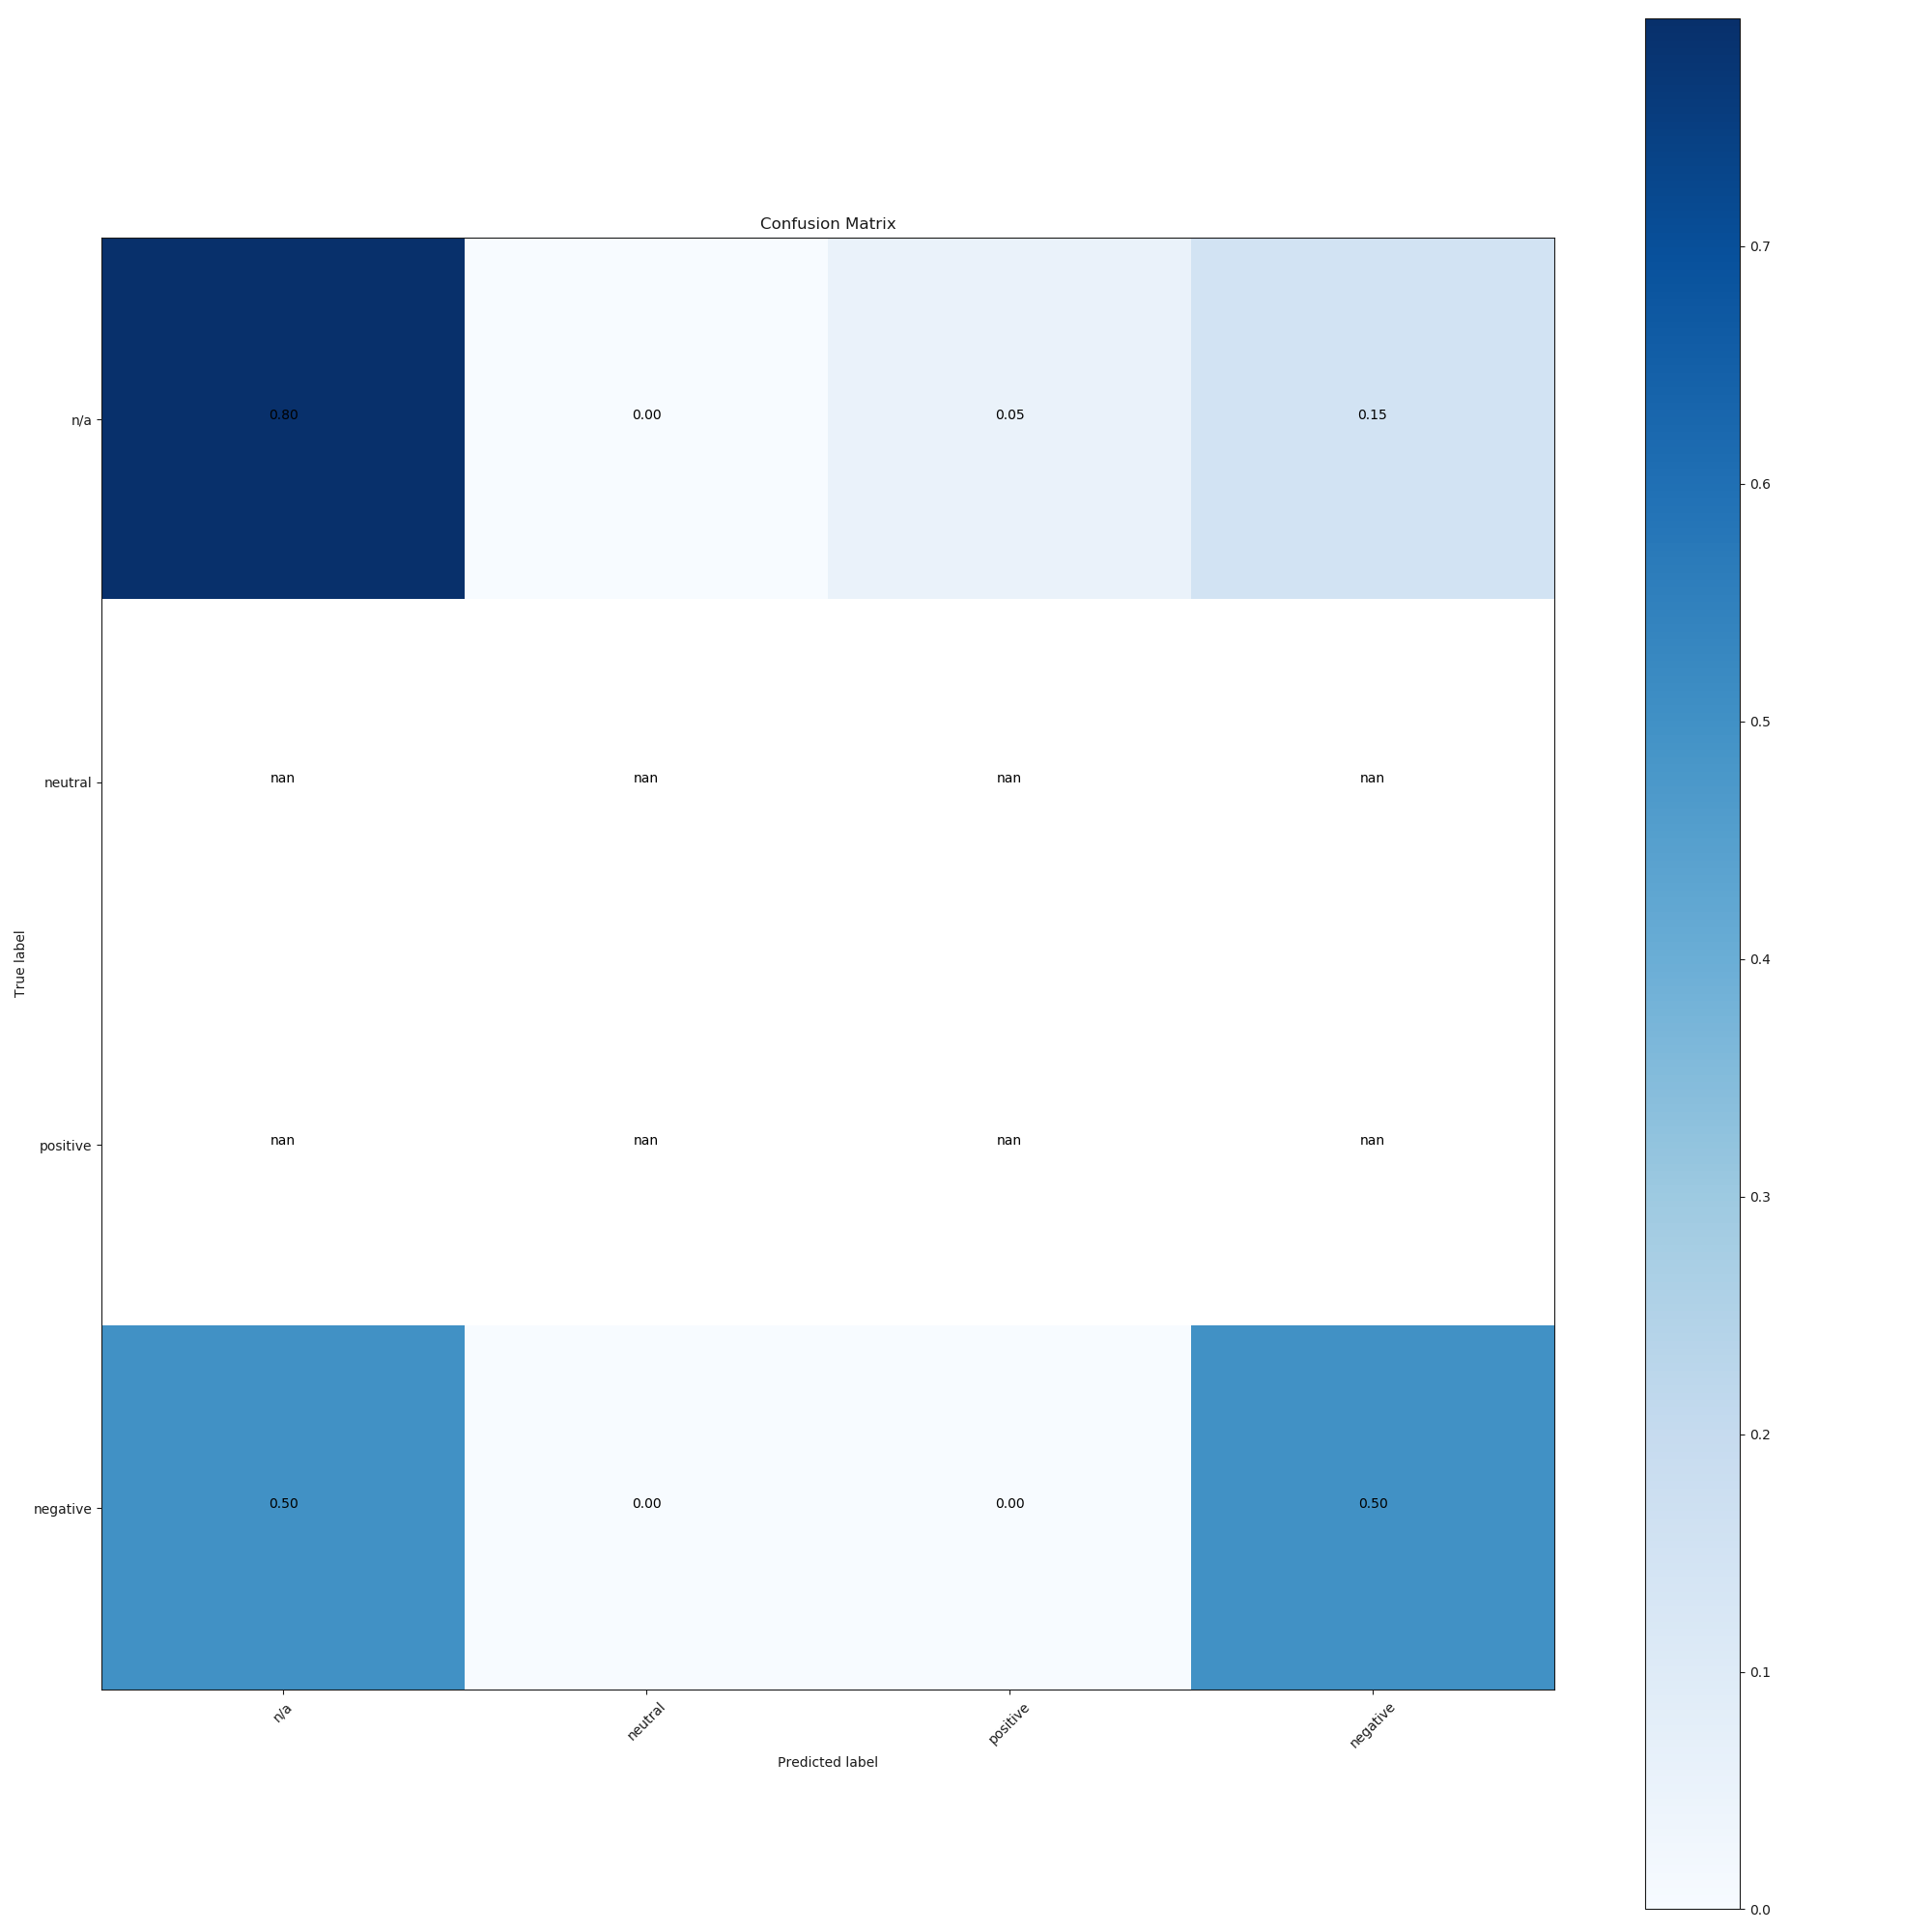
\includegraphics[width=0.19\textwidth]{figures/08_appendix/organic/08_1}
    }
    \subfloat[Conventional:Quality]{
        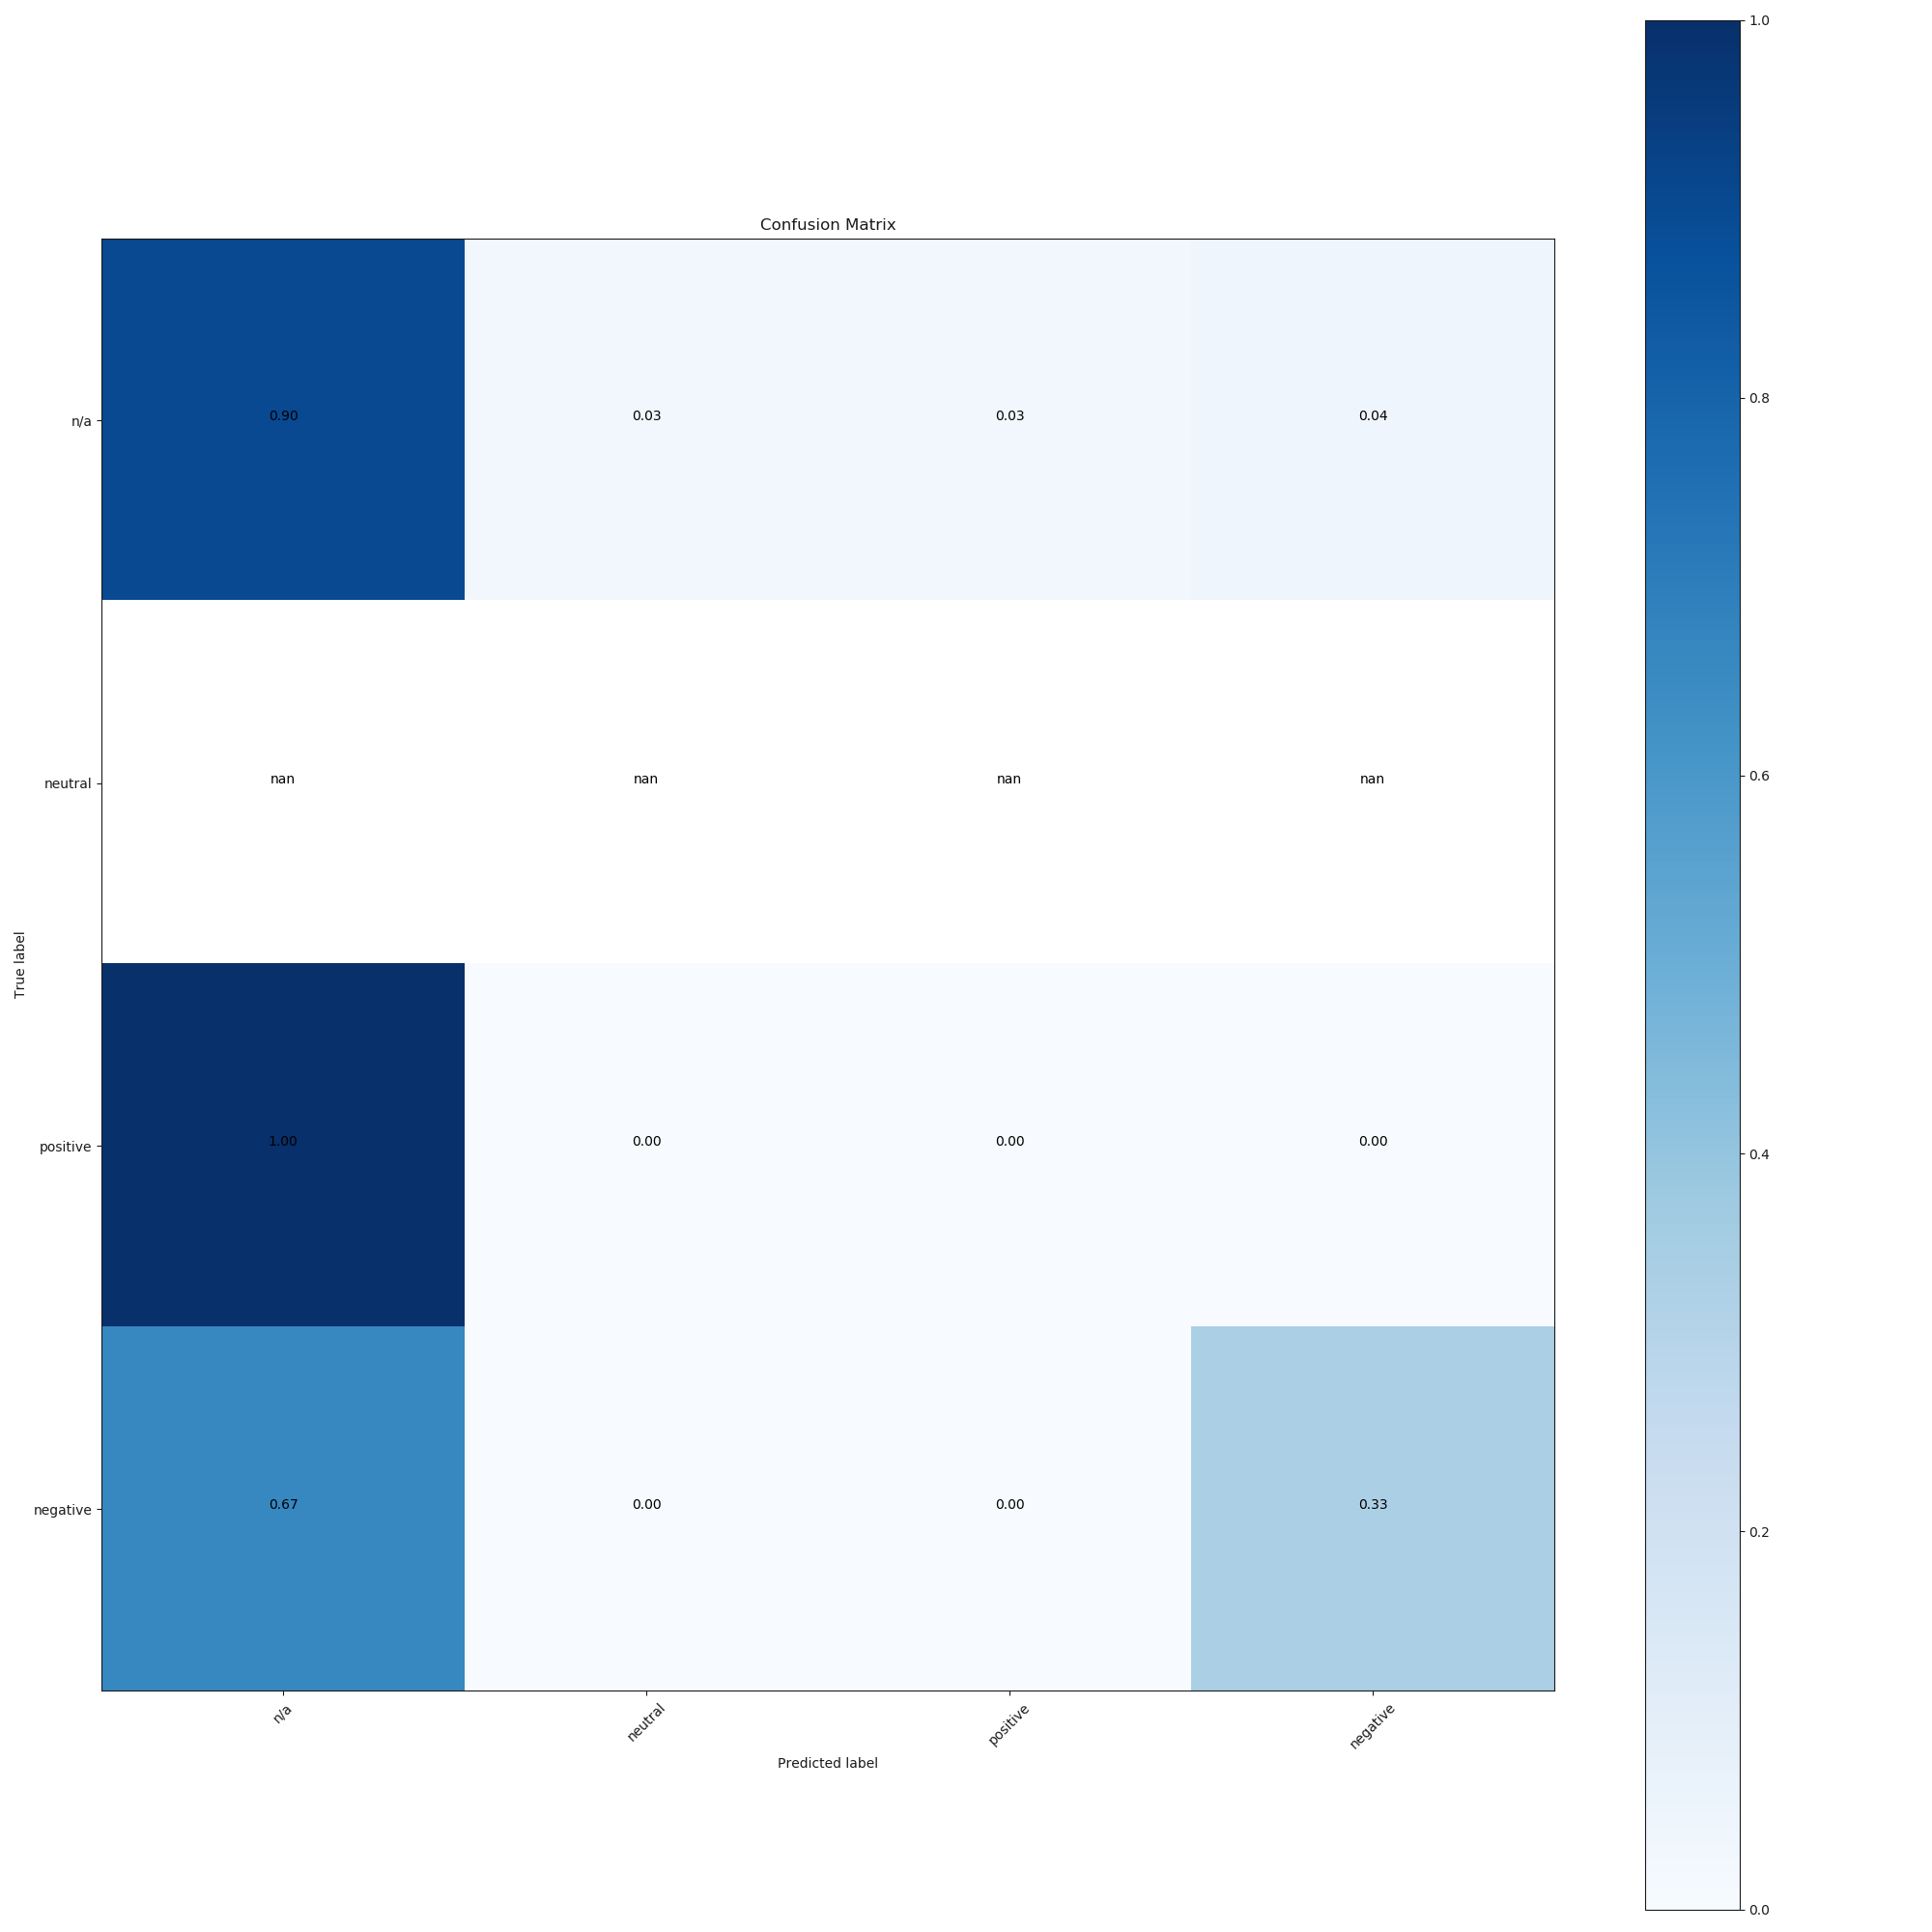
\includegraphics[width=0.19\textwidth]{figures/08_appendix/organic/08_2}
    }
    \subfloat[Conventional:General]{
        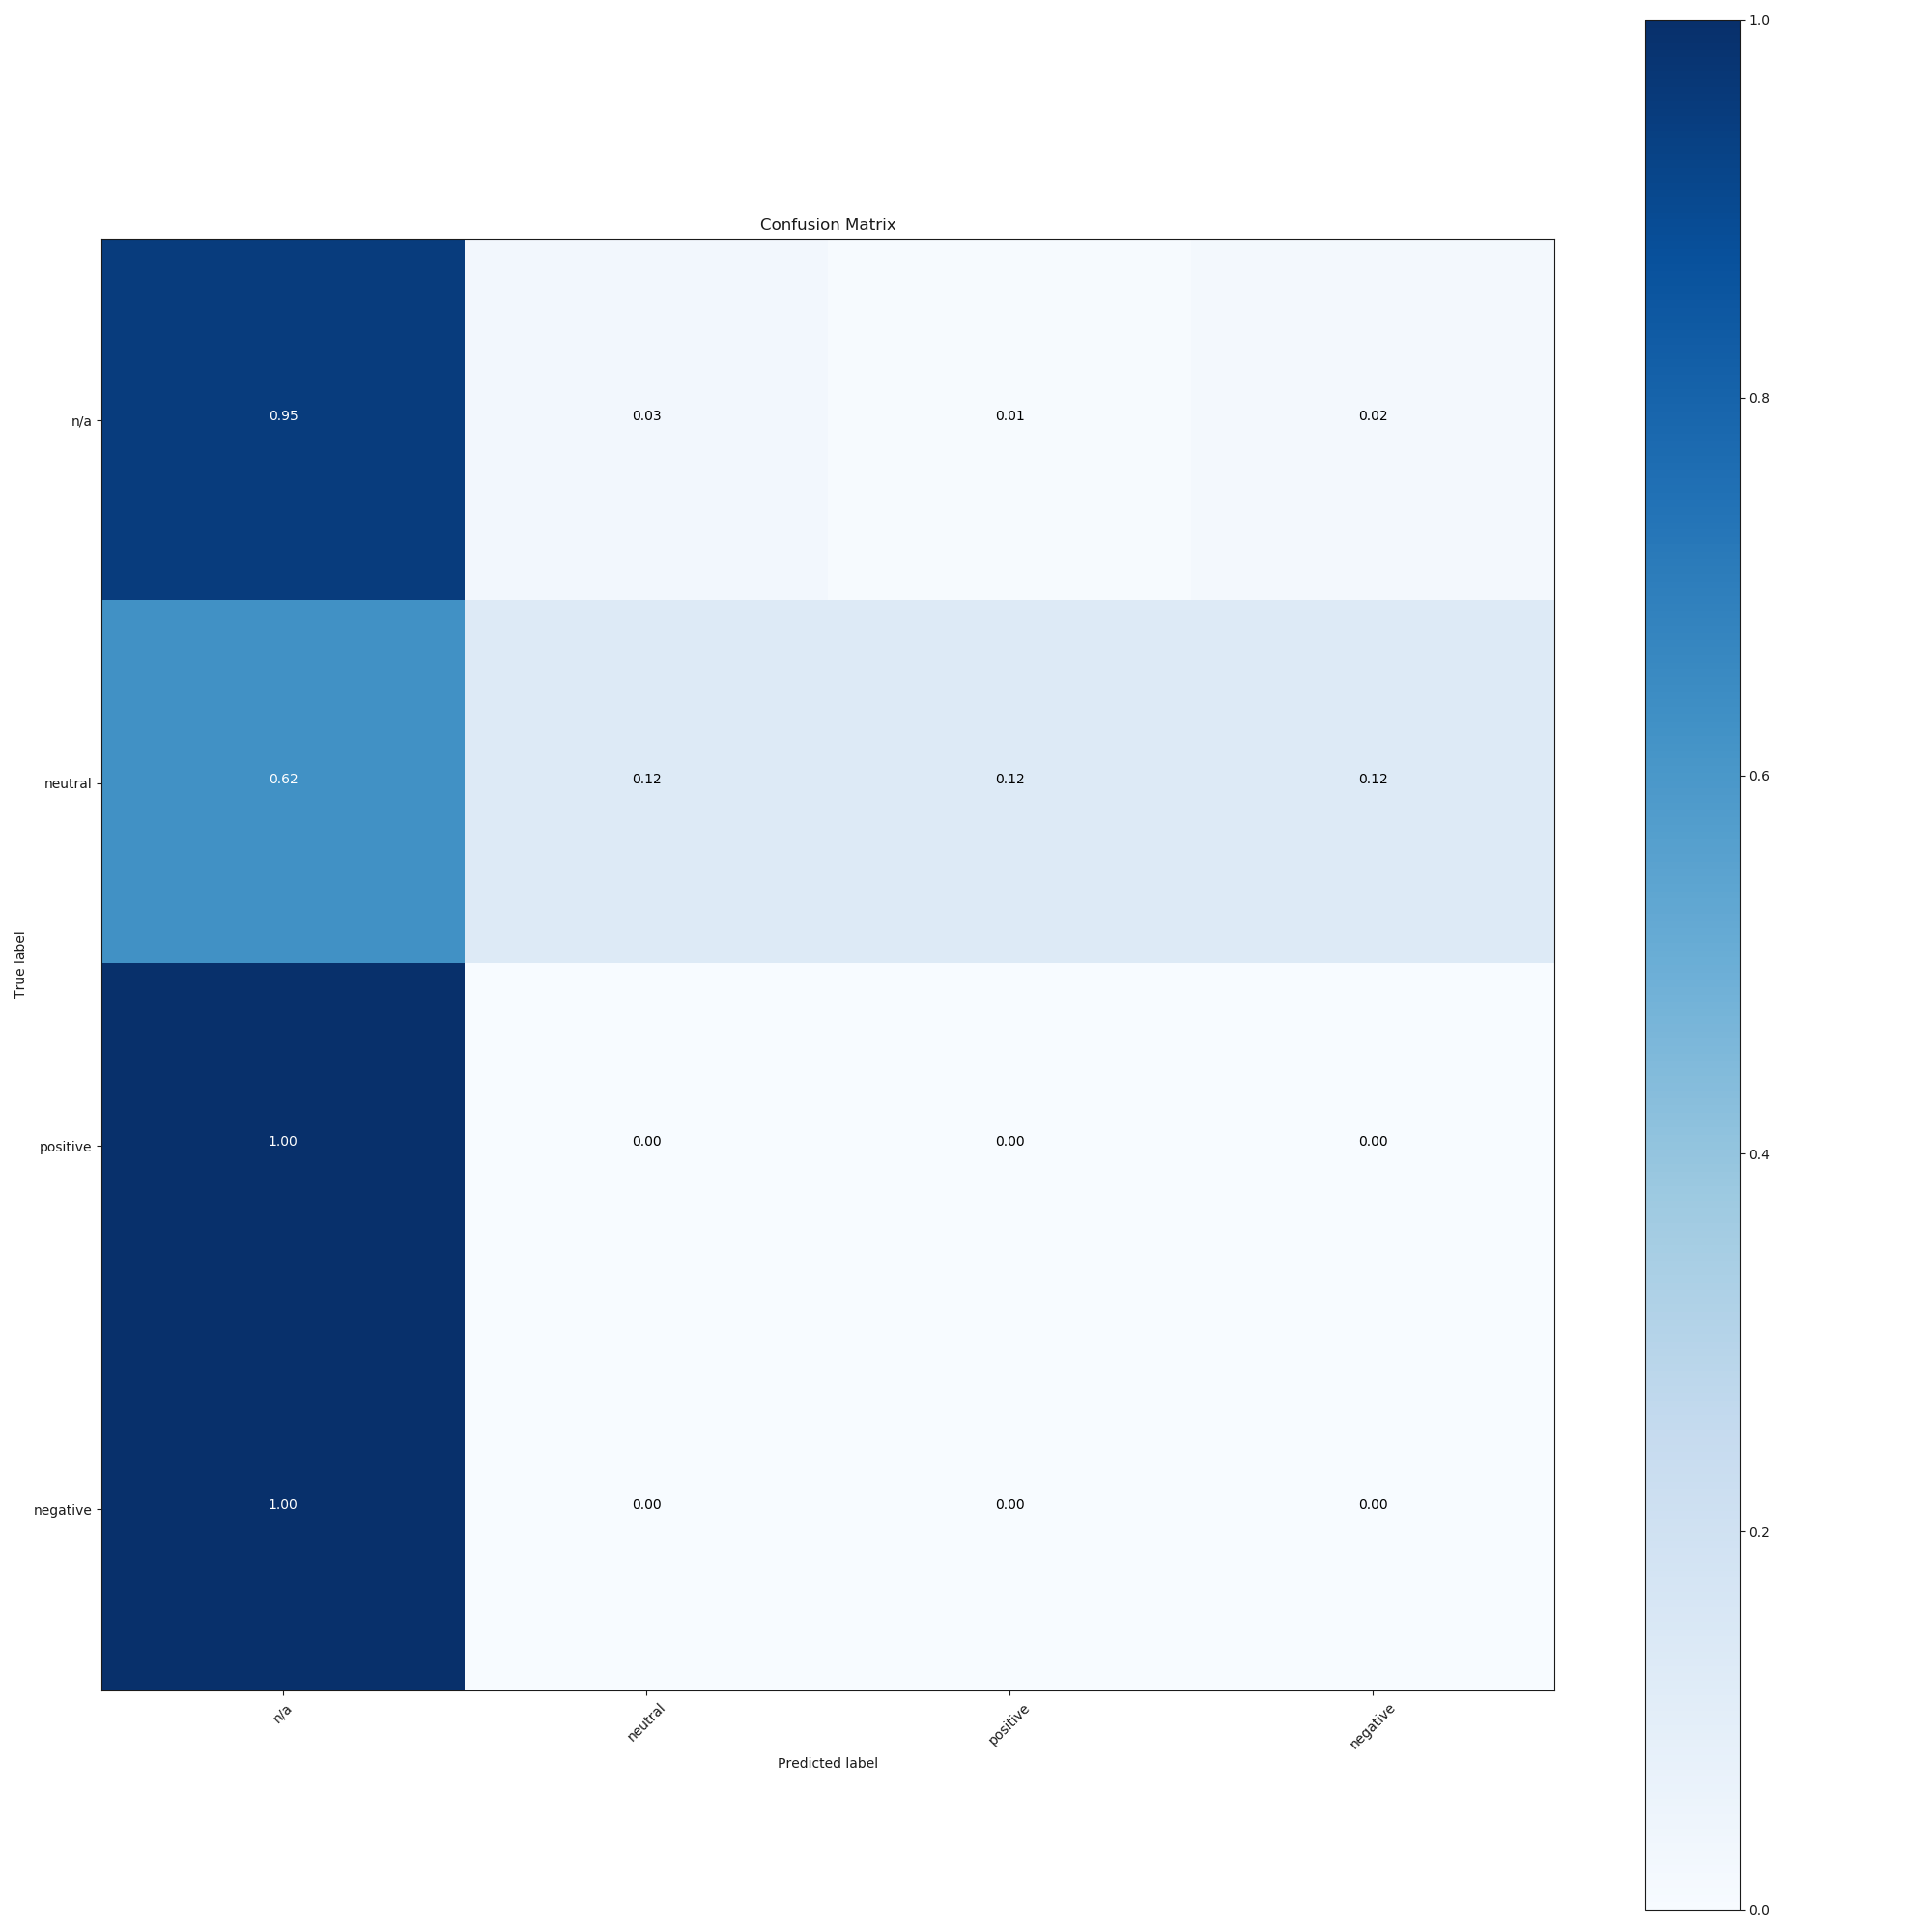
\includegraphics[width=0.19\textwidth]{figures/08_appendix/organic/08_3}
    }
    \subfloat[Conventional:Price]{
        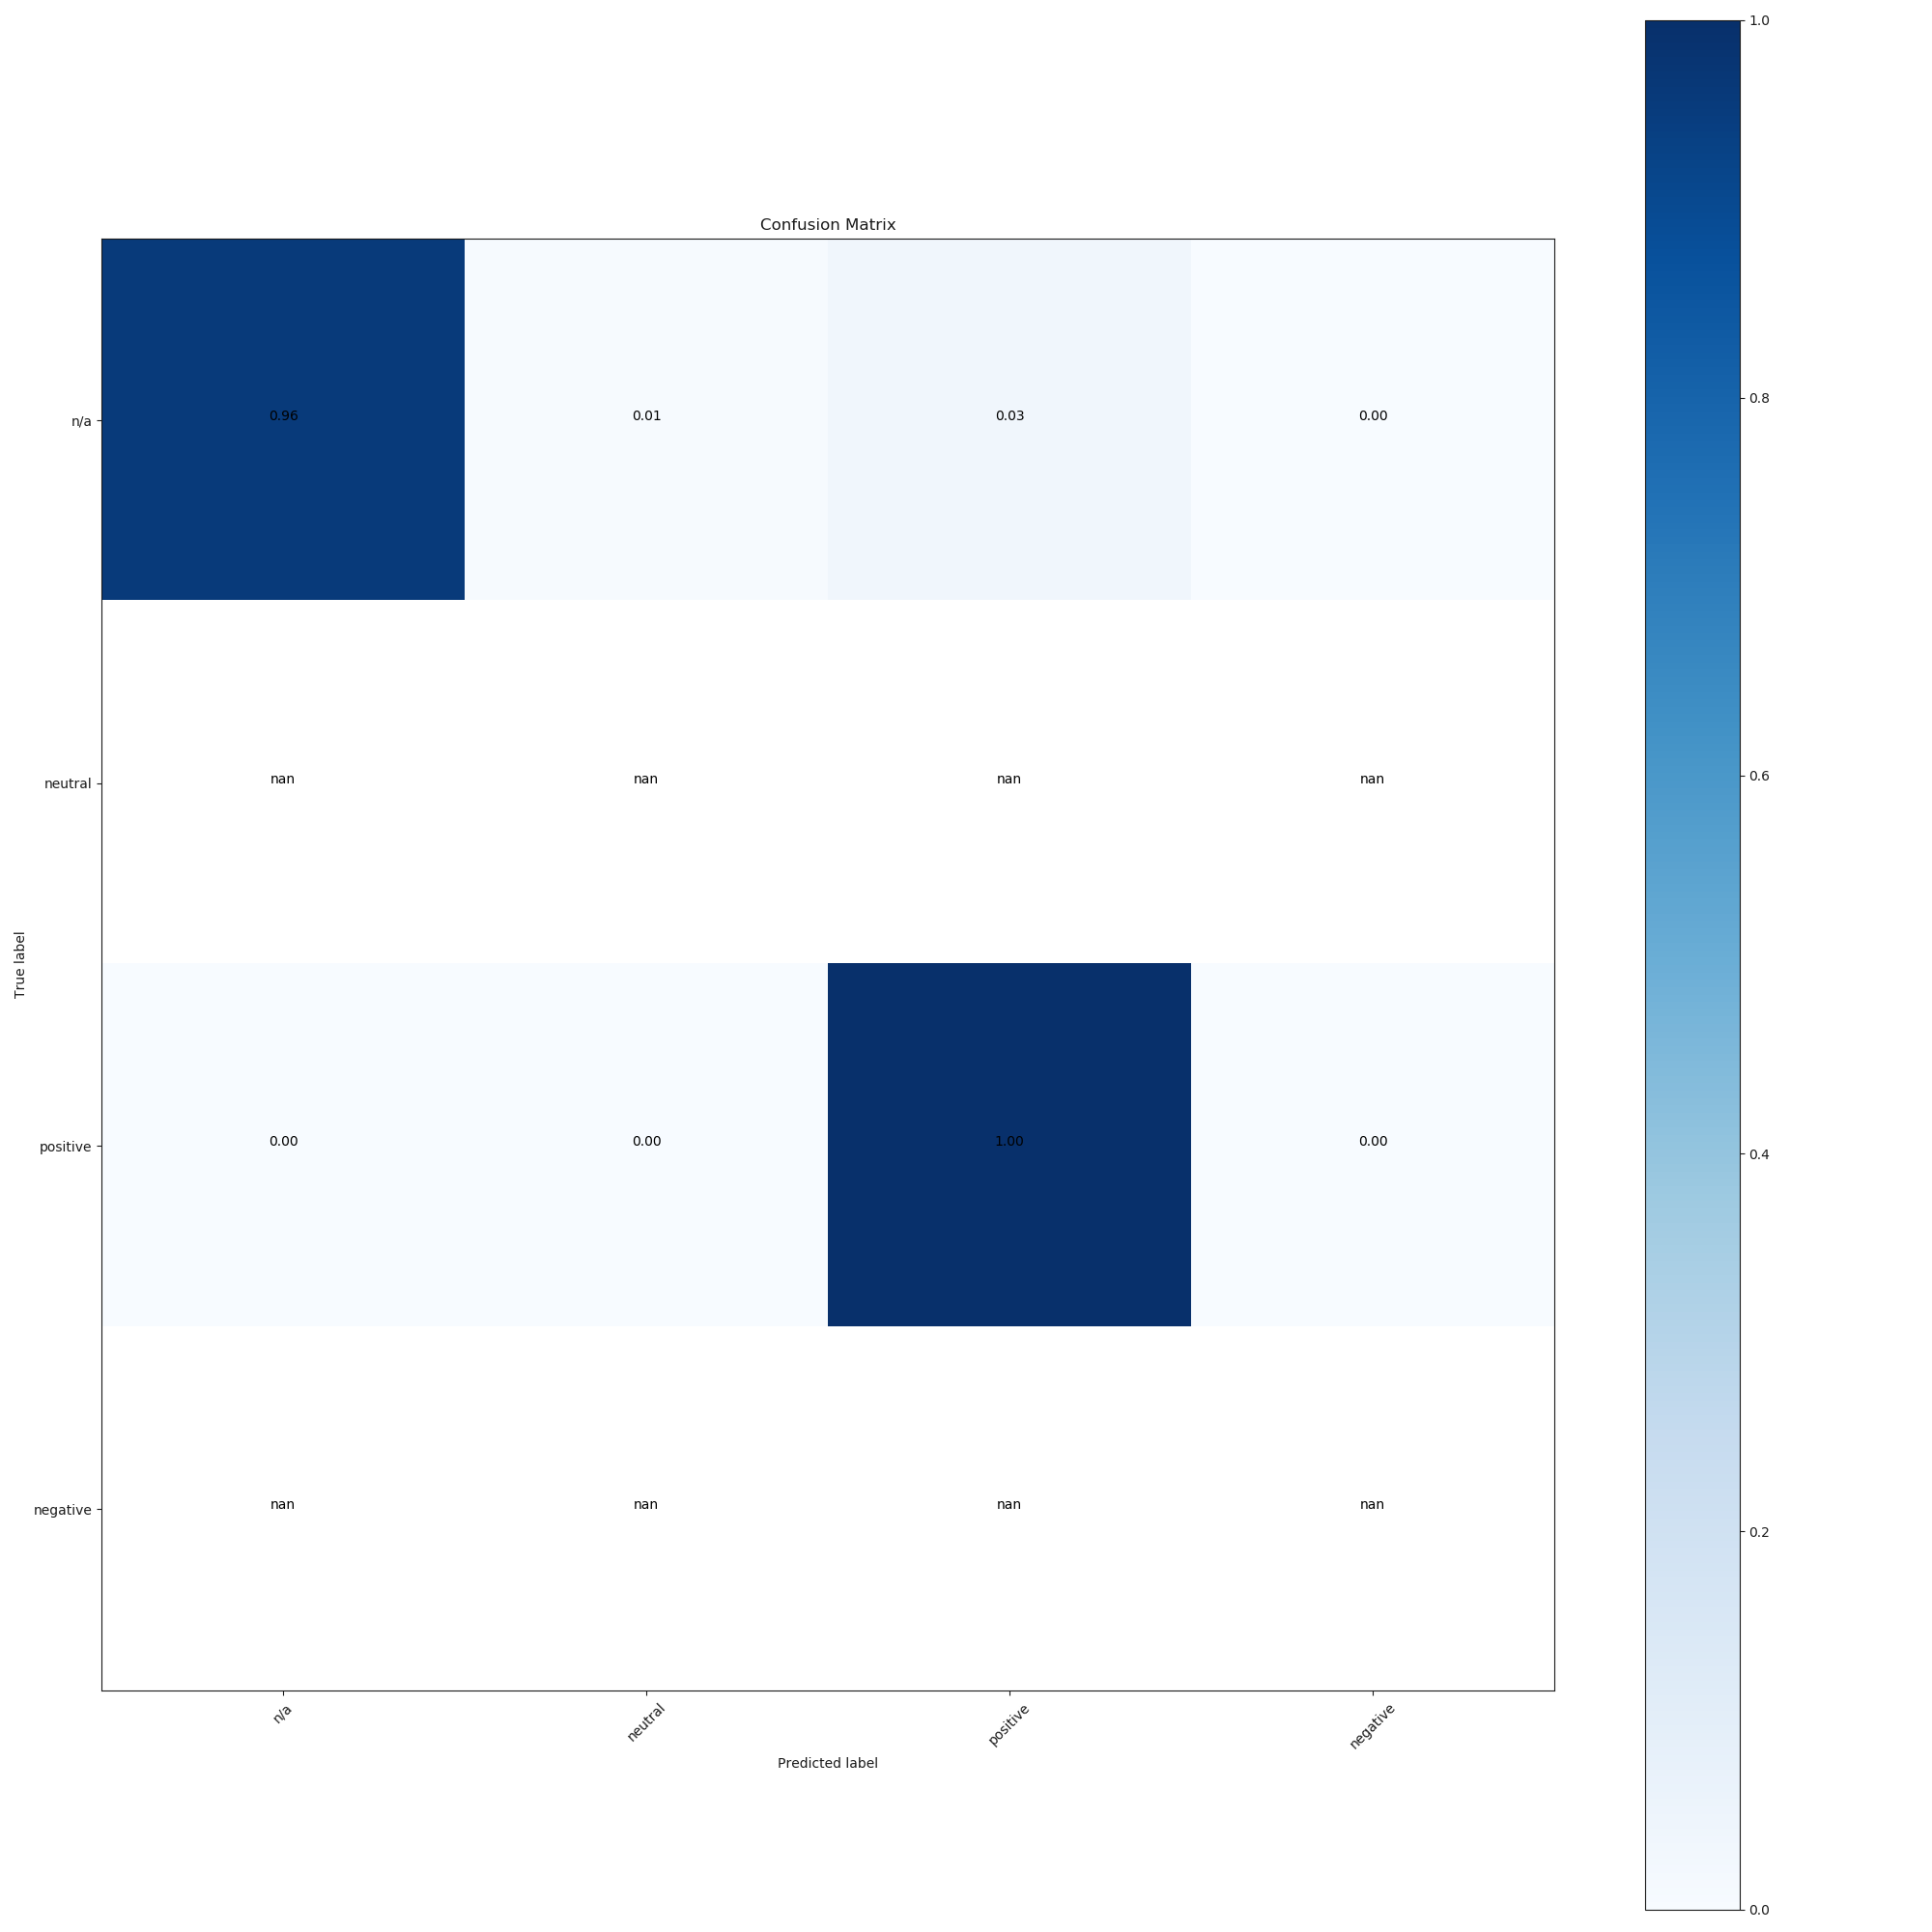
\includegraphics[width=0.19\textwidth]{figures/08_appendix/organic/08_4}
    }
    \subfloat[Conventional:Safety]{
        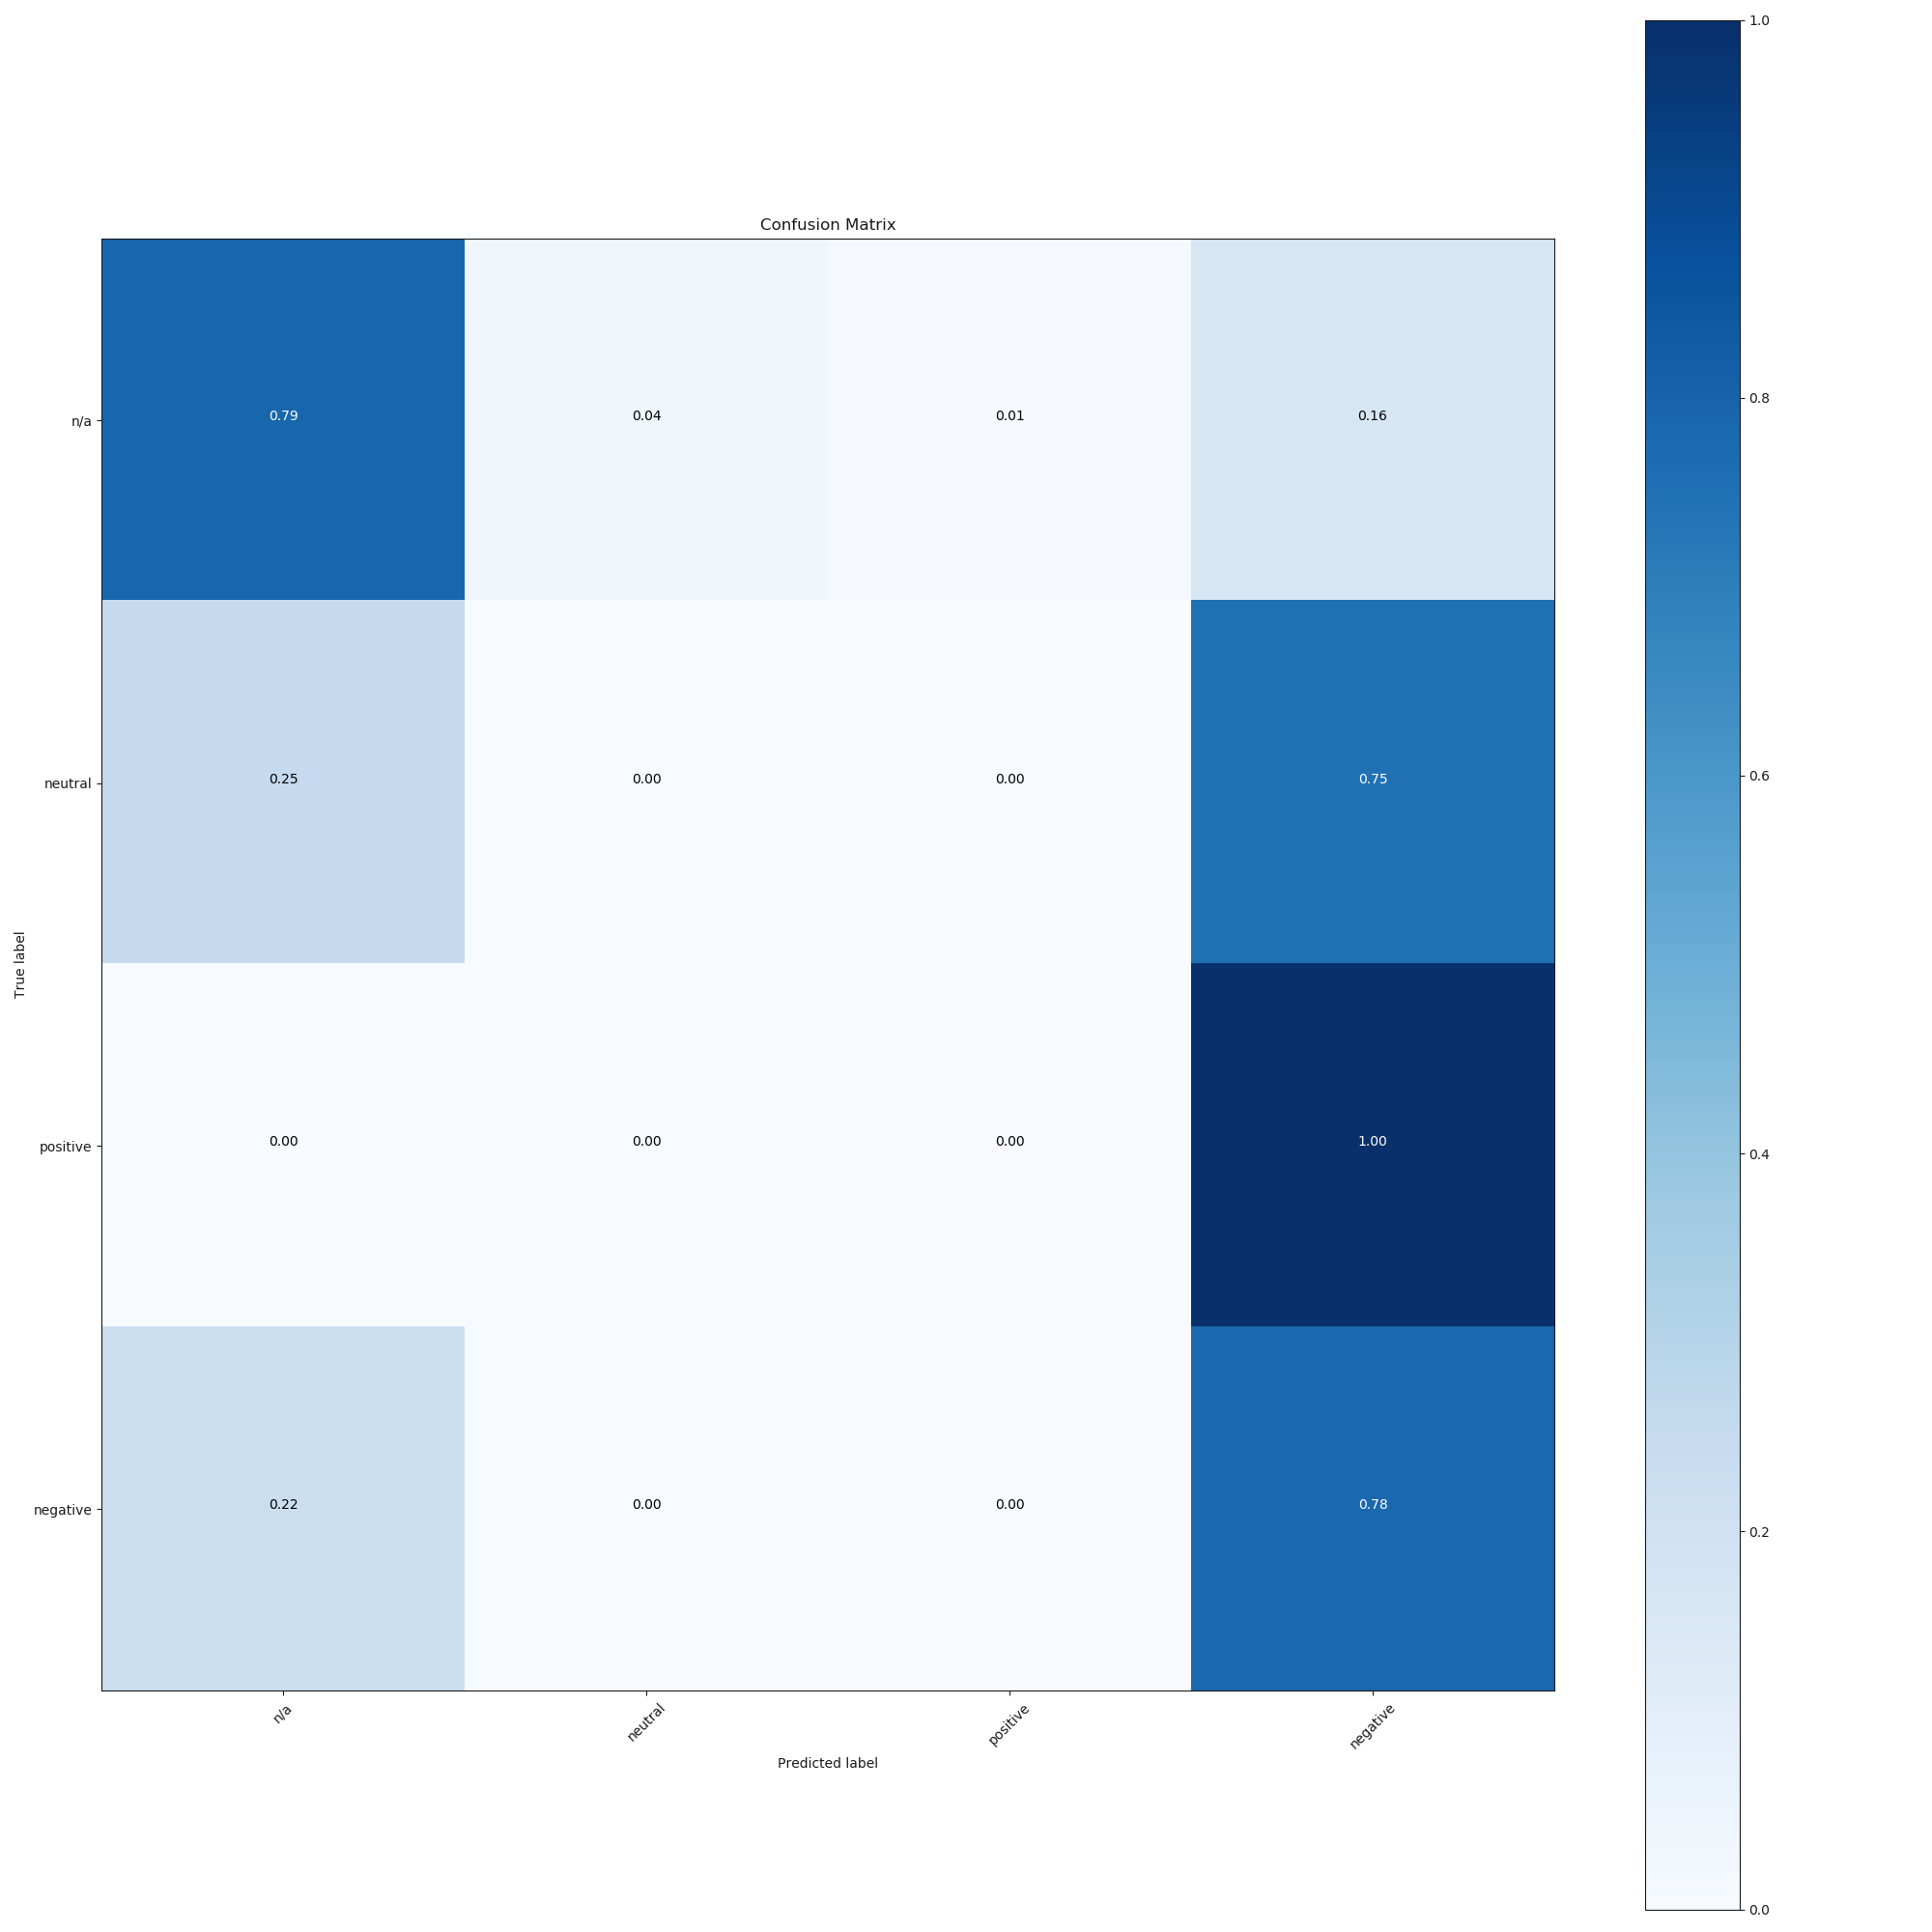
\includegraphics[width=0.19\textwidth]{figures/08_appendix/organic/08_5}
    }
    \hspace{0mm}

    \subfloat[Conventional:Sources]{
        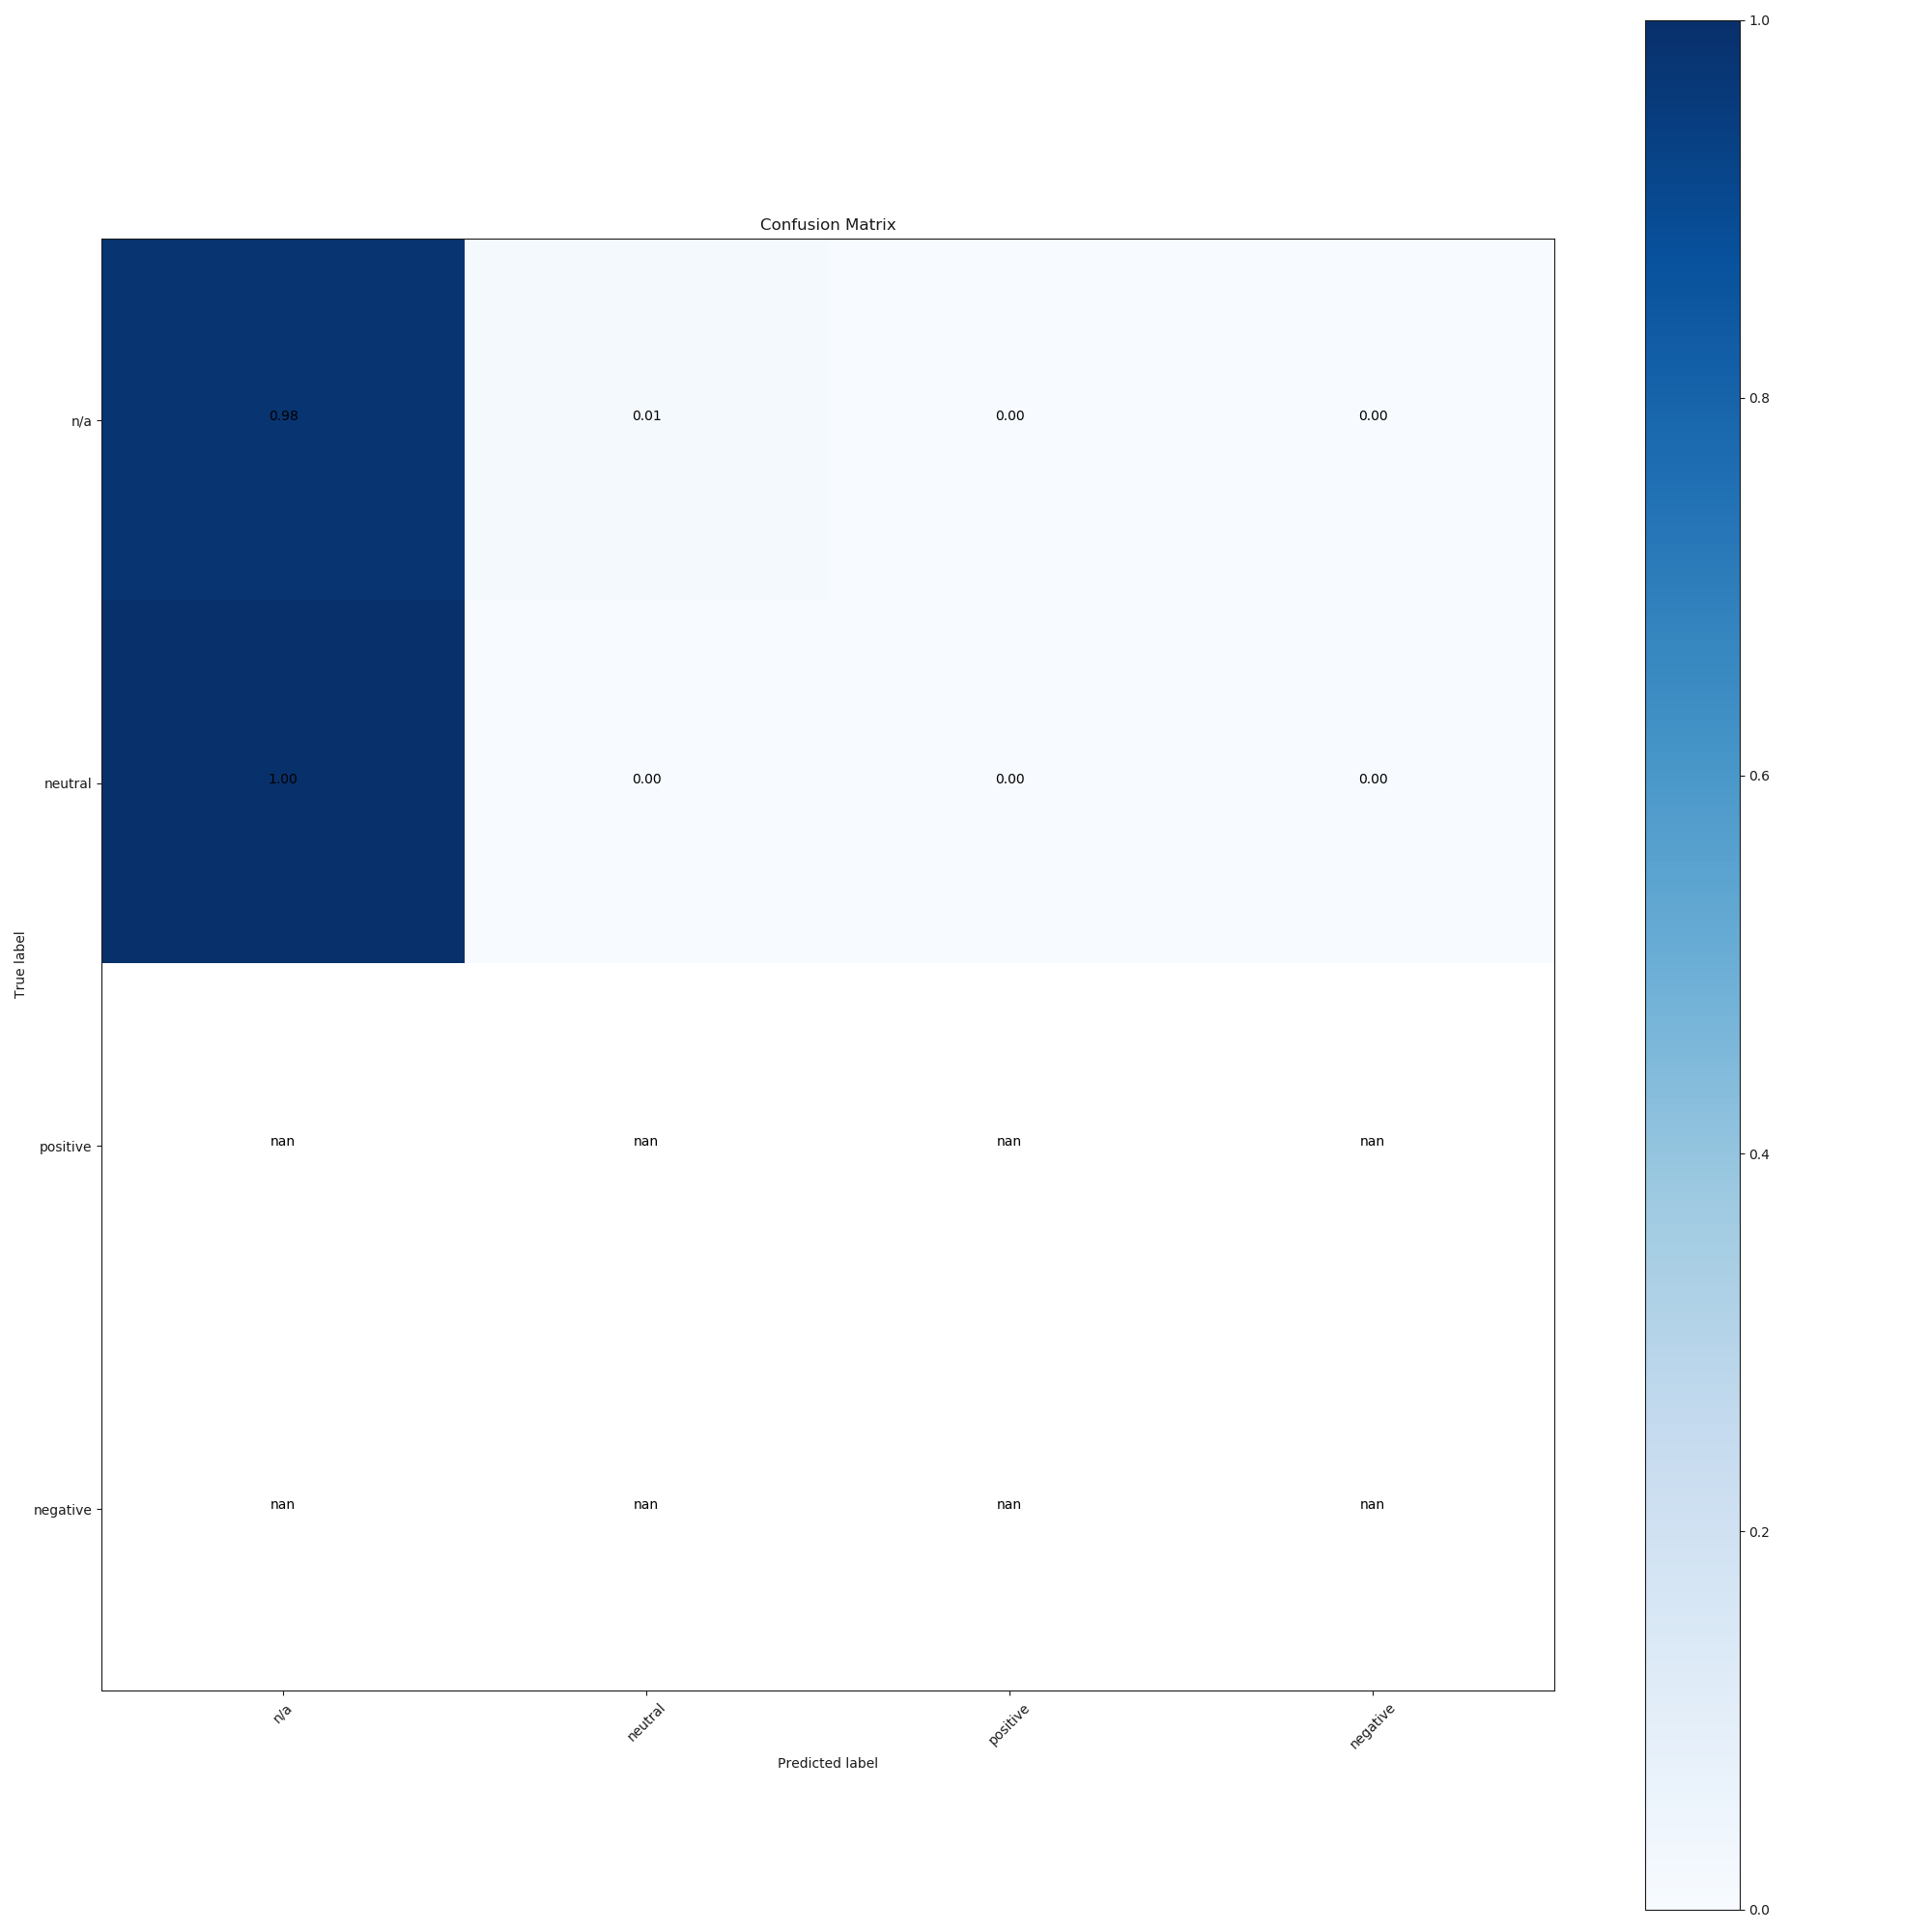
\includegraphics[width=0.19\textwidth]{figures/08_appendix/organic/08_6}
    }
    \subfloat[GMO:Environment]{
        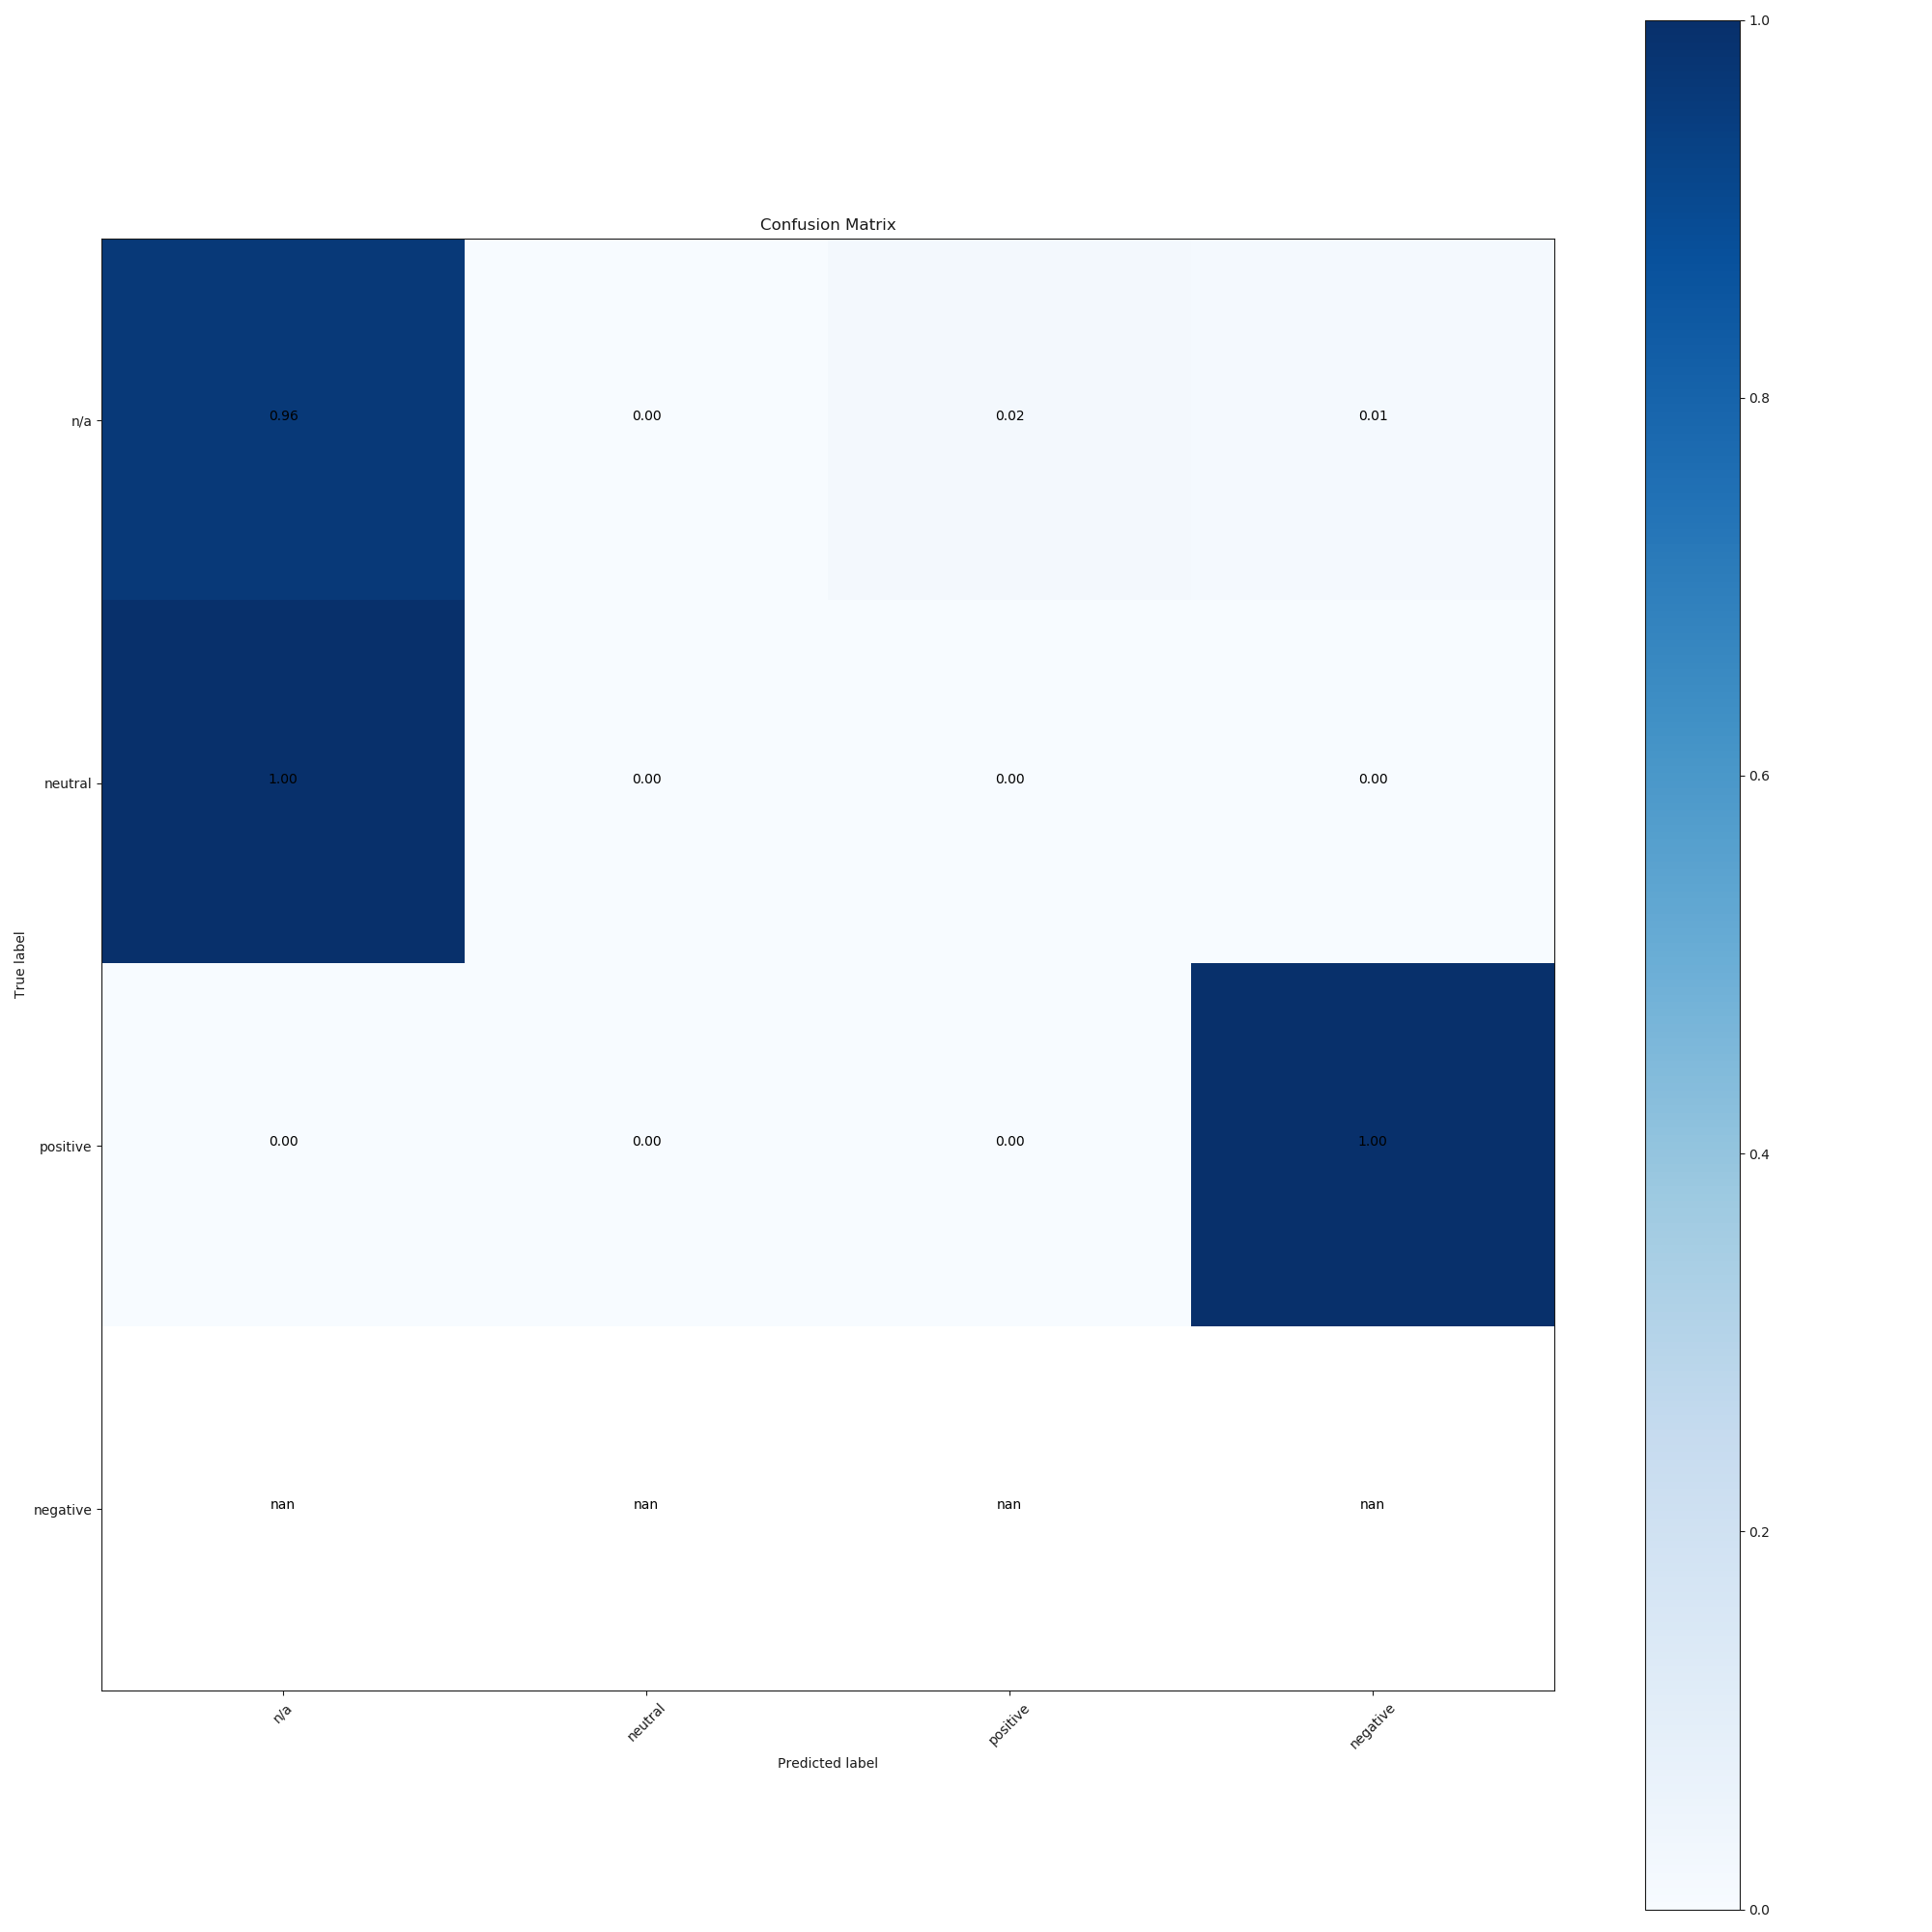
\includegraphics[width=0.19\textwidth]{figures/08_appendix/organic/08_7}
    }
    \subfloat[GMO:Quality]{
        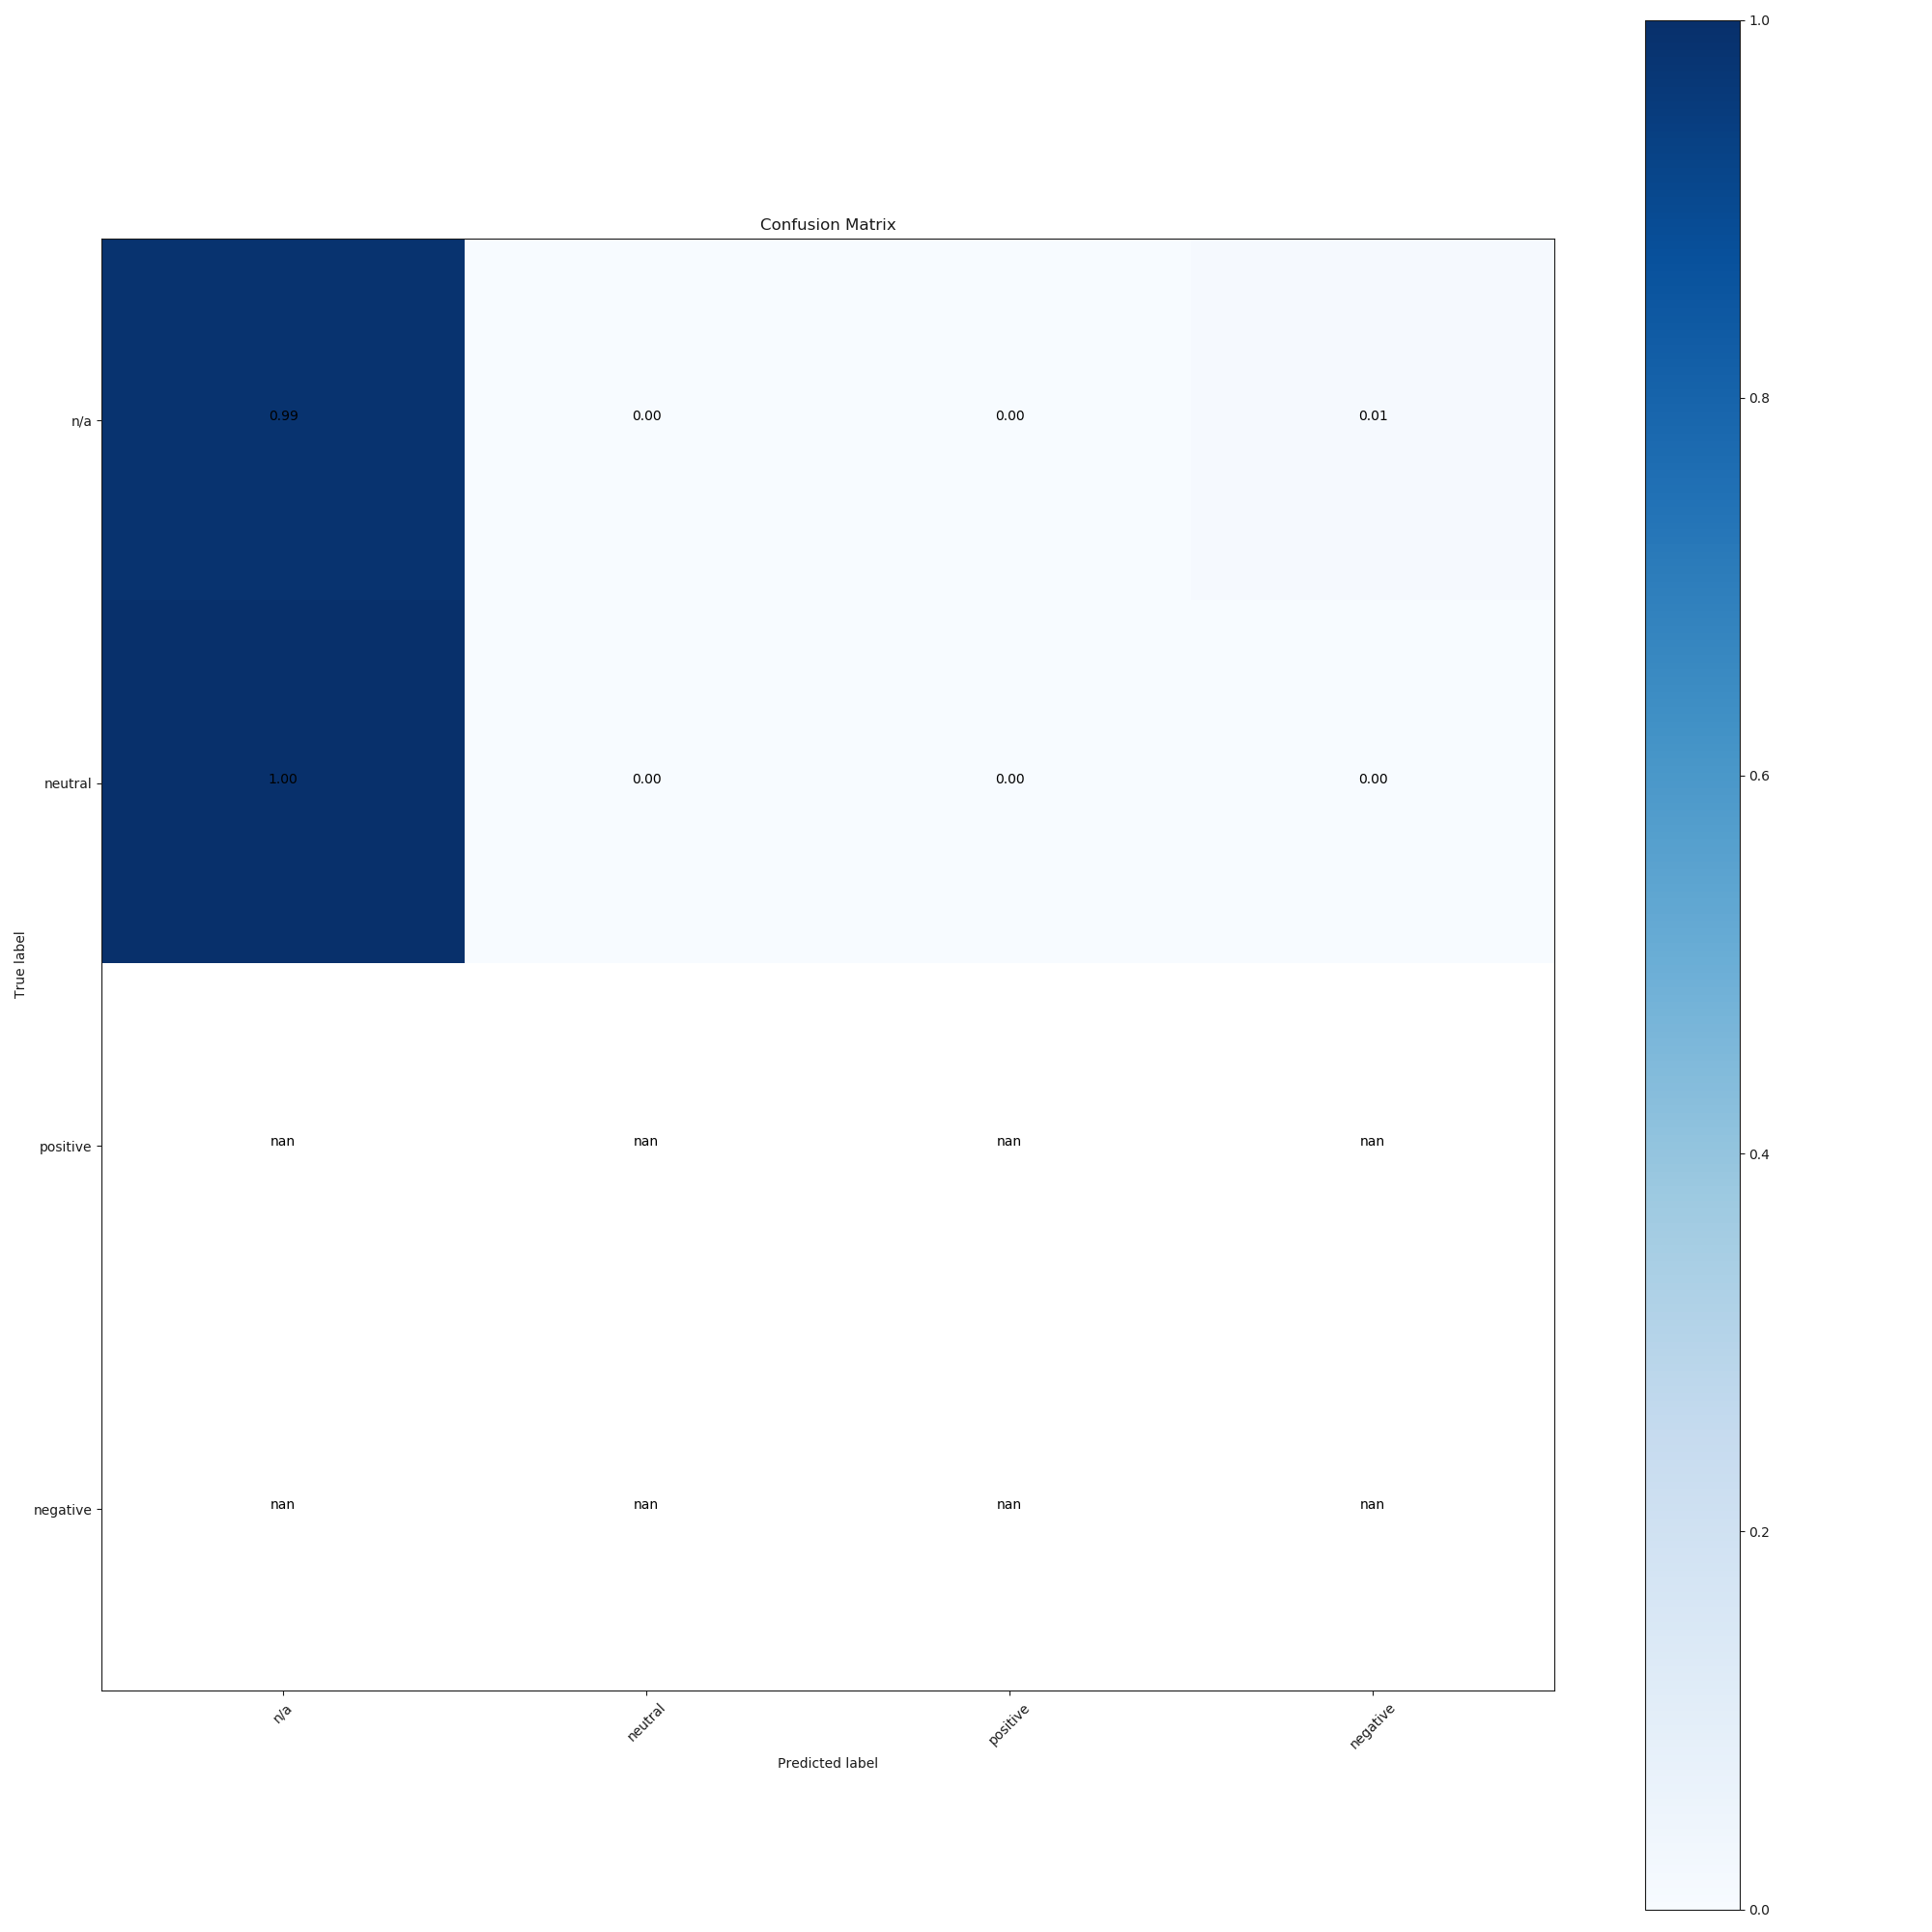
\includegraphics[width=0.19\textwidth]{figures/08_appendix/organic/08_8}
    }
    \subfloat[GMO:General]{
        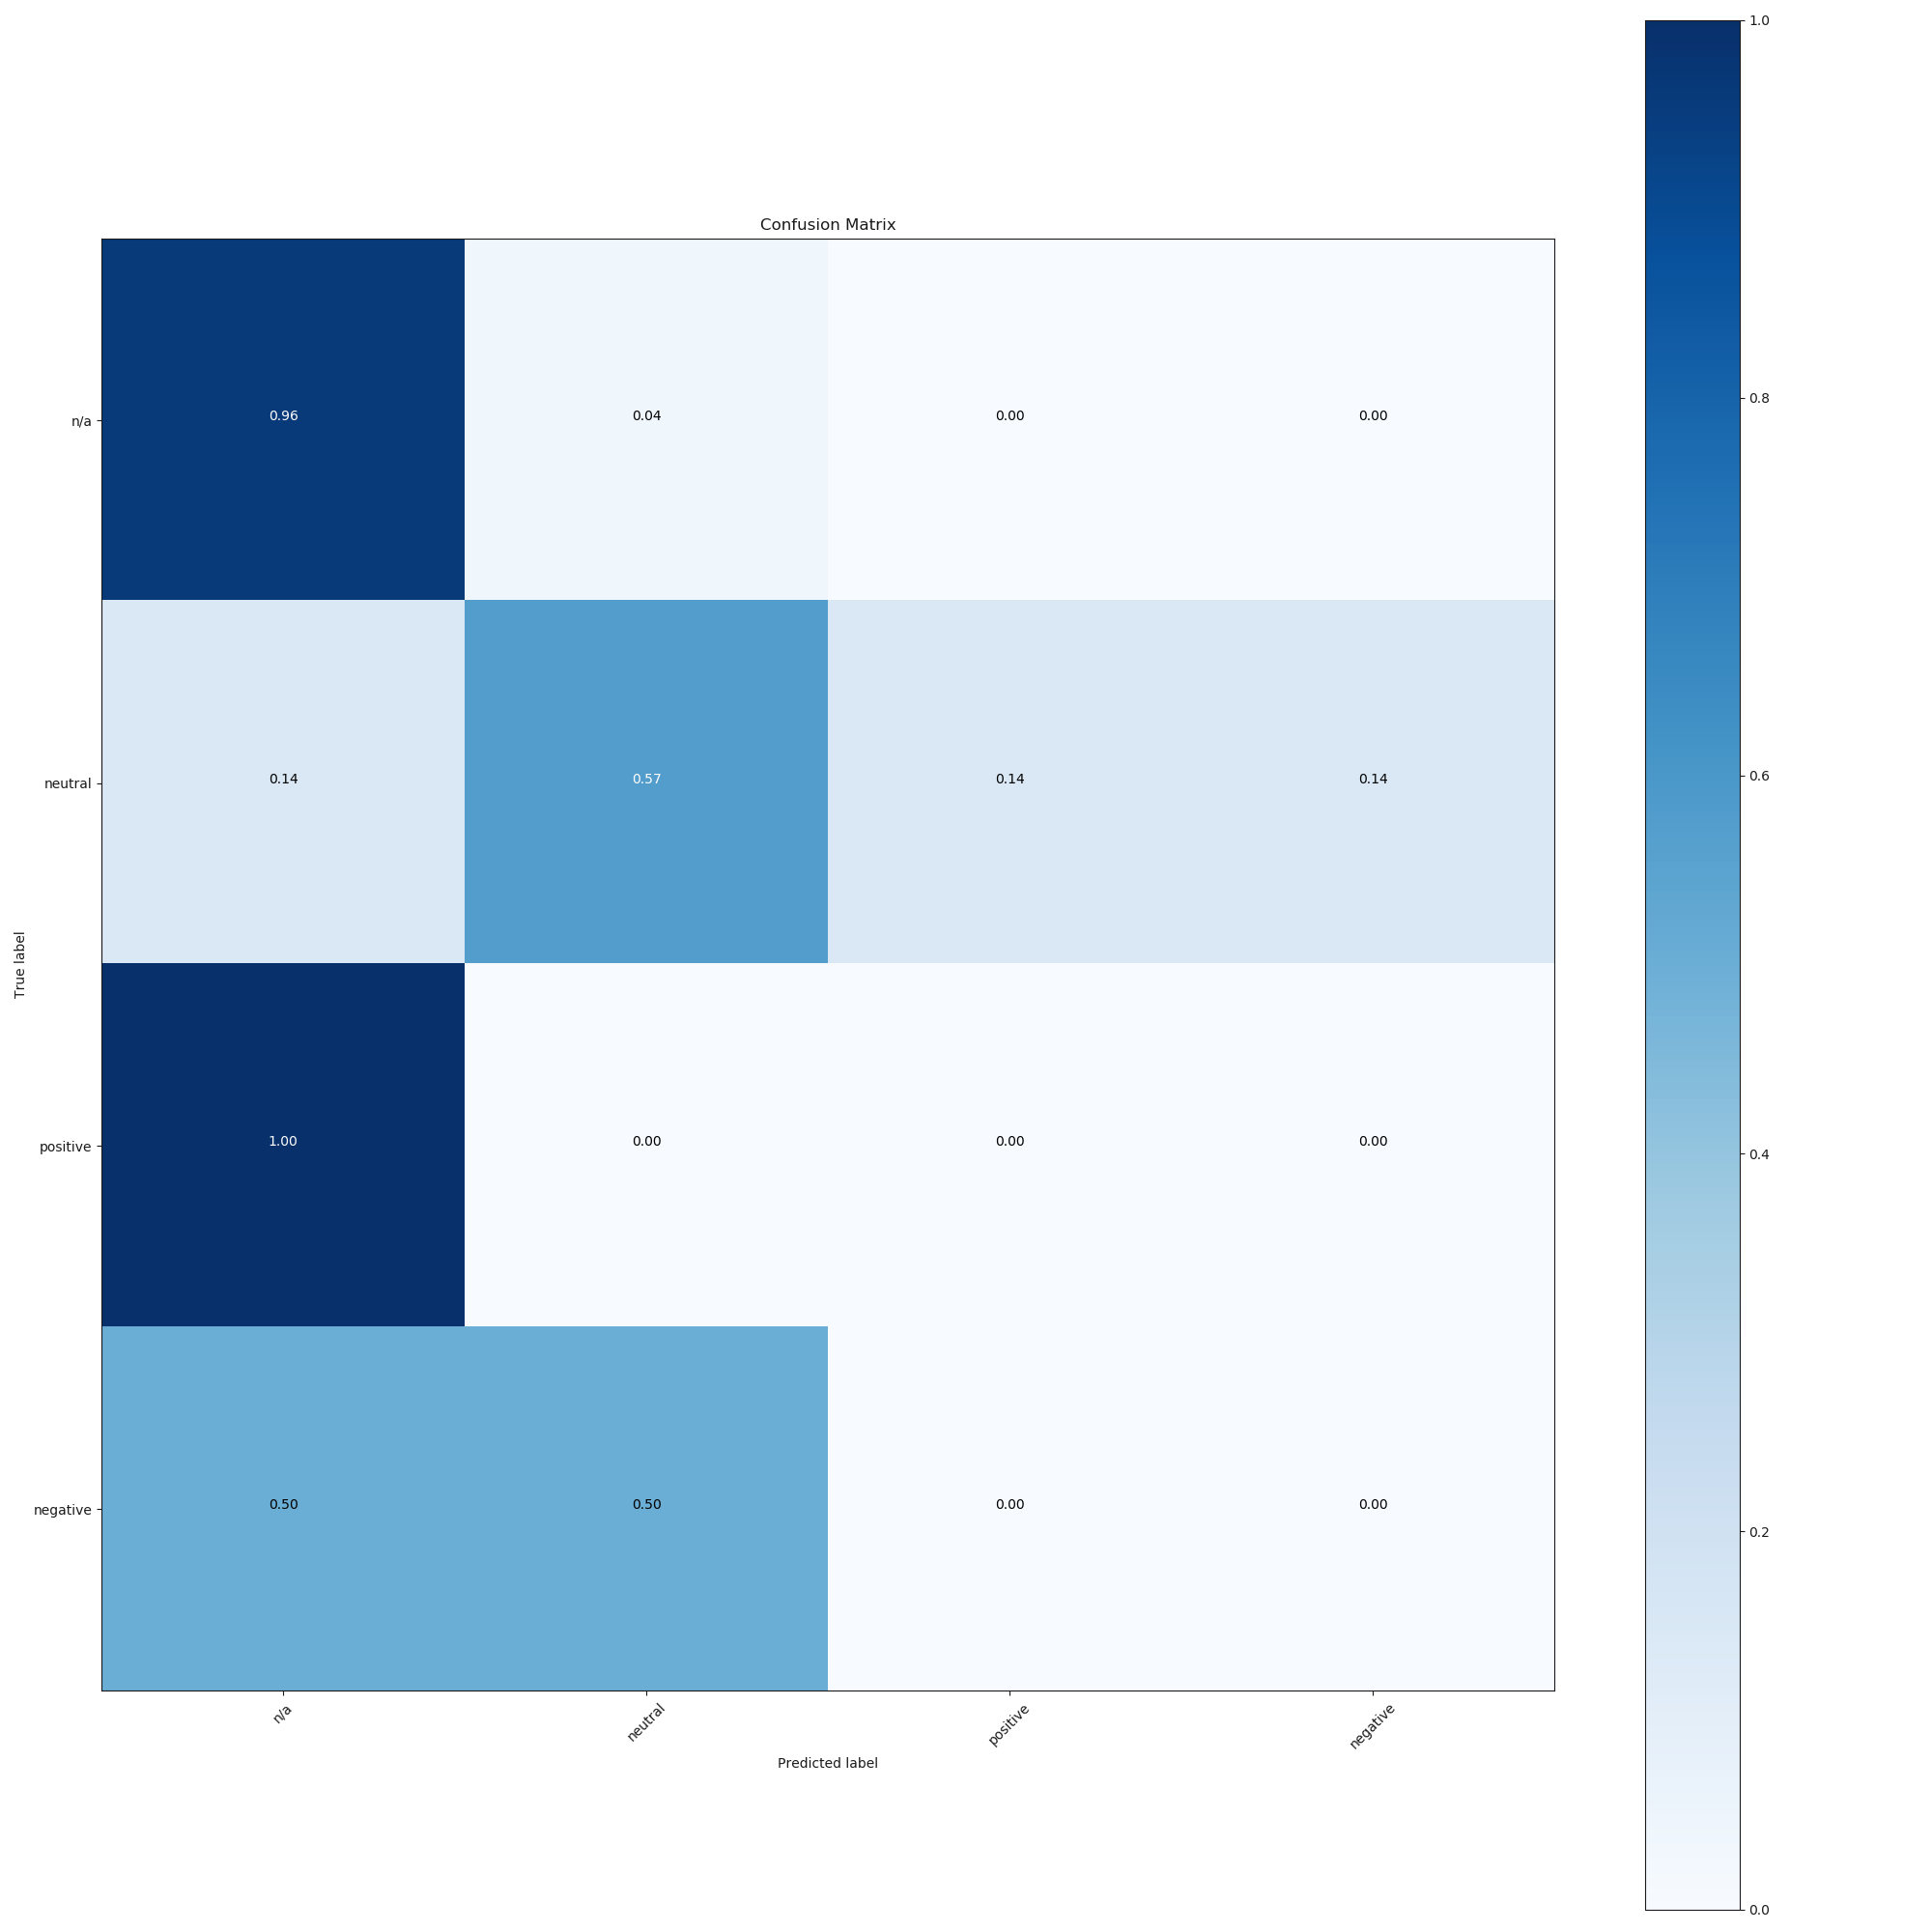
\includegraphics[width=0.19\textwidth]{figures/08_appendix/organic/08_9}
    }
    \subfloat[GMO:Price]{
        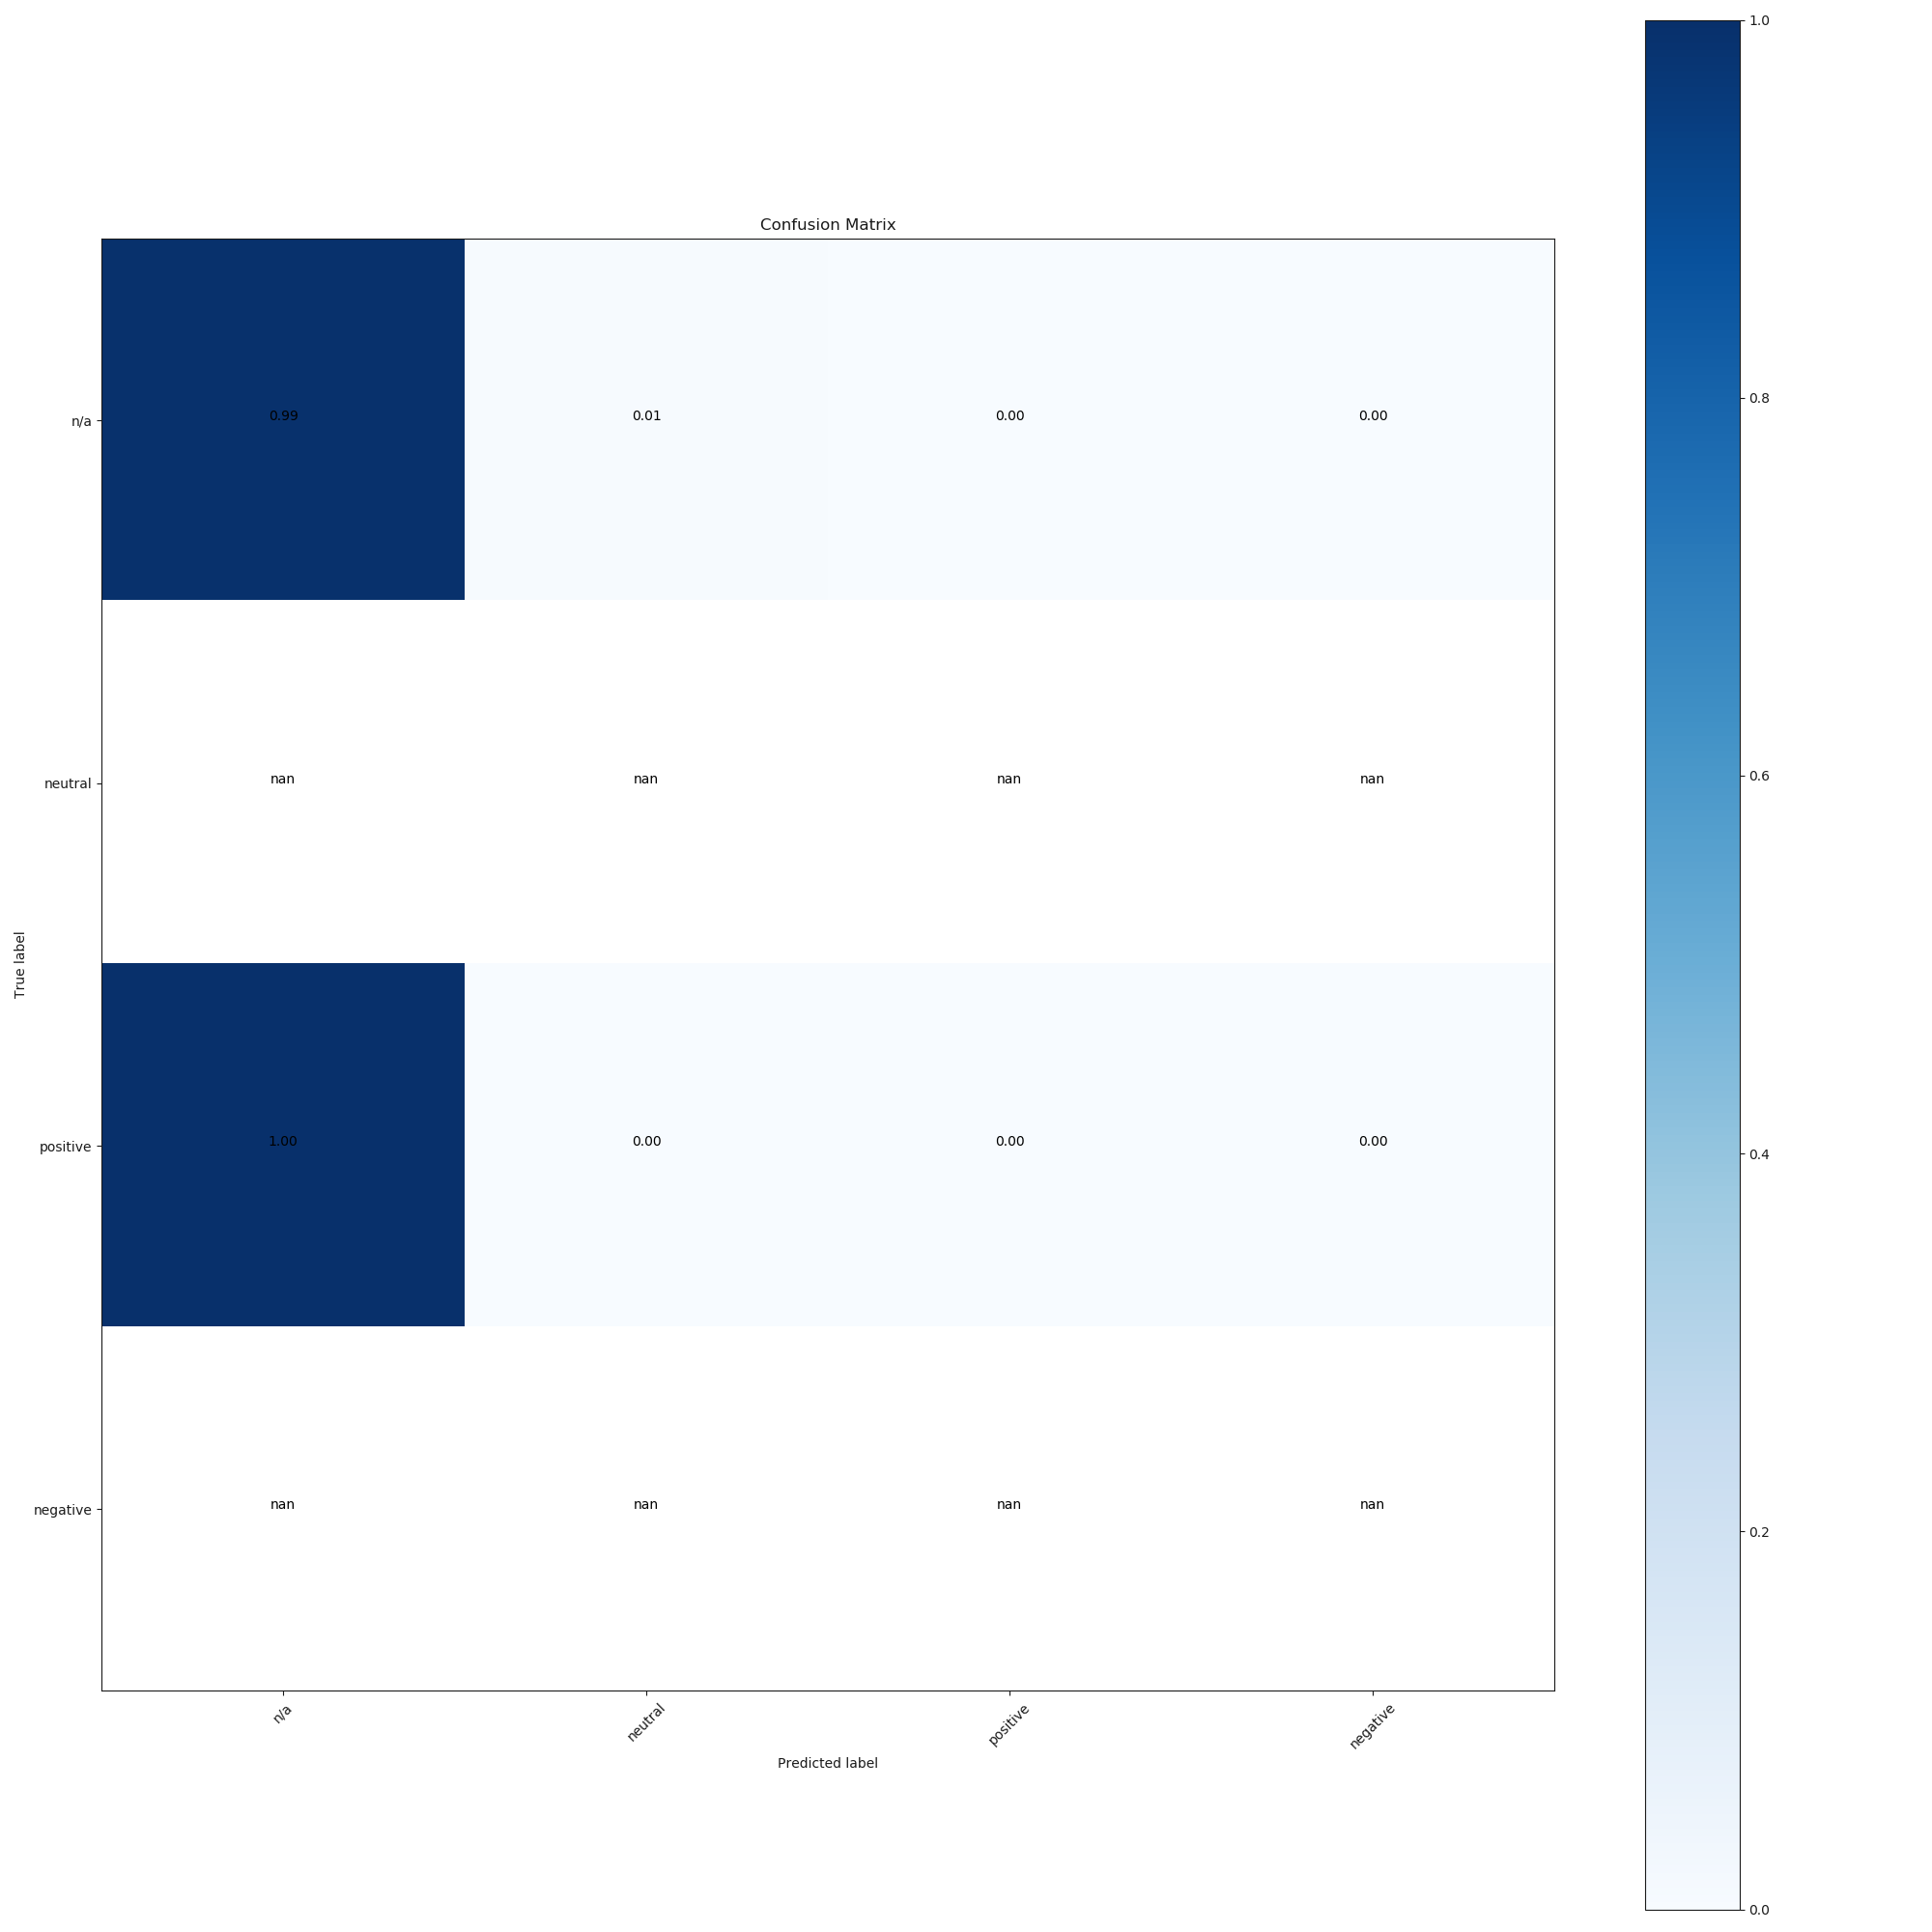
\includegraphics[width=0.19\textwidth]{figures/08_appendix/organic/08_10}
    }
    \hspace{0mm}

    \subfloat[GMO:Safety]{
        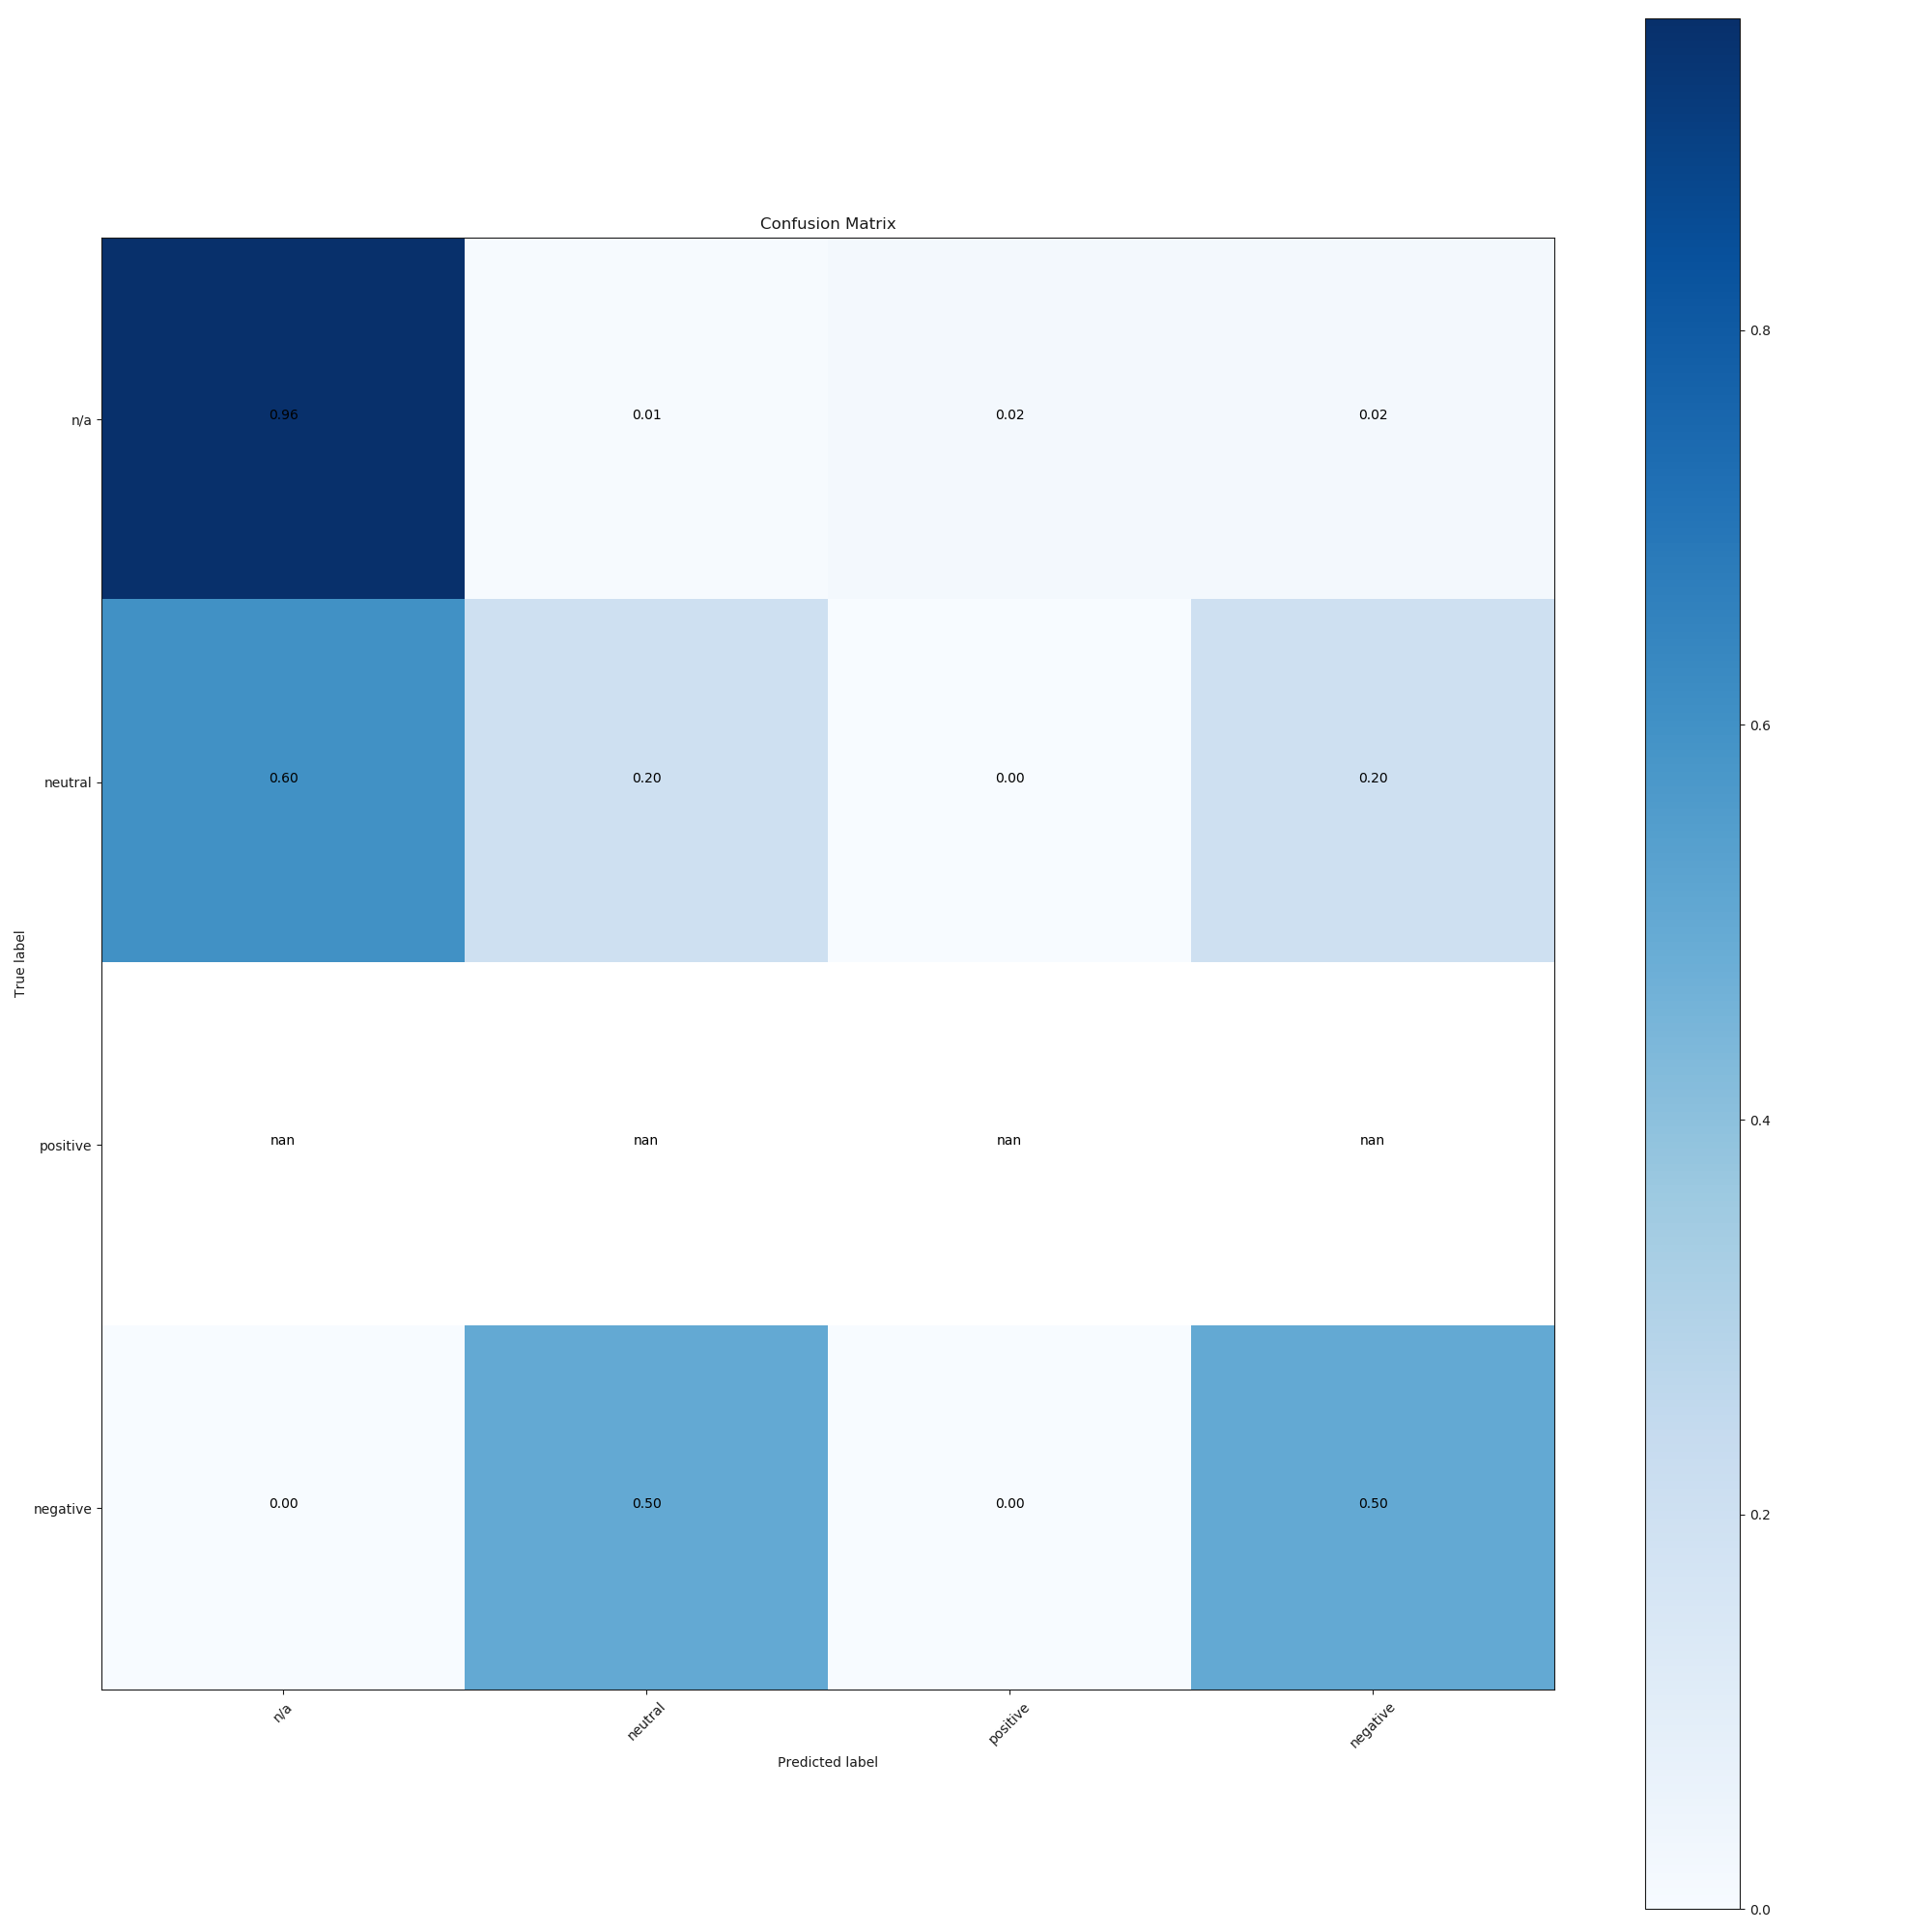
\includegraphics[width=0.19\textwidth]{figures/08_appendix/organic/08_11}
    }
    \subfloat[GMO:Sources]{
        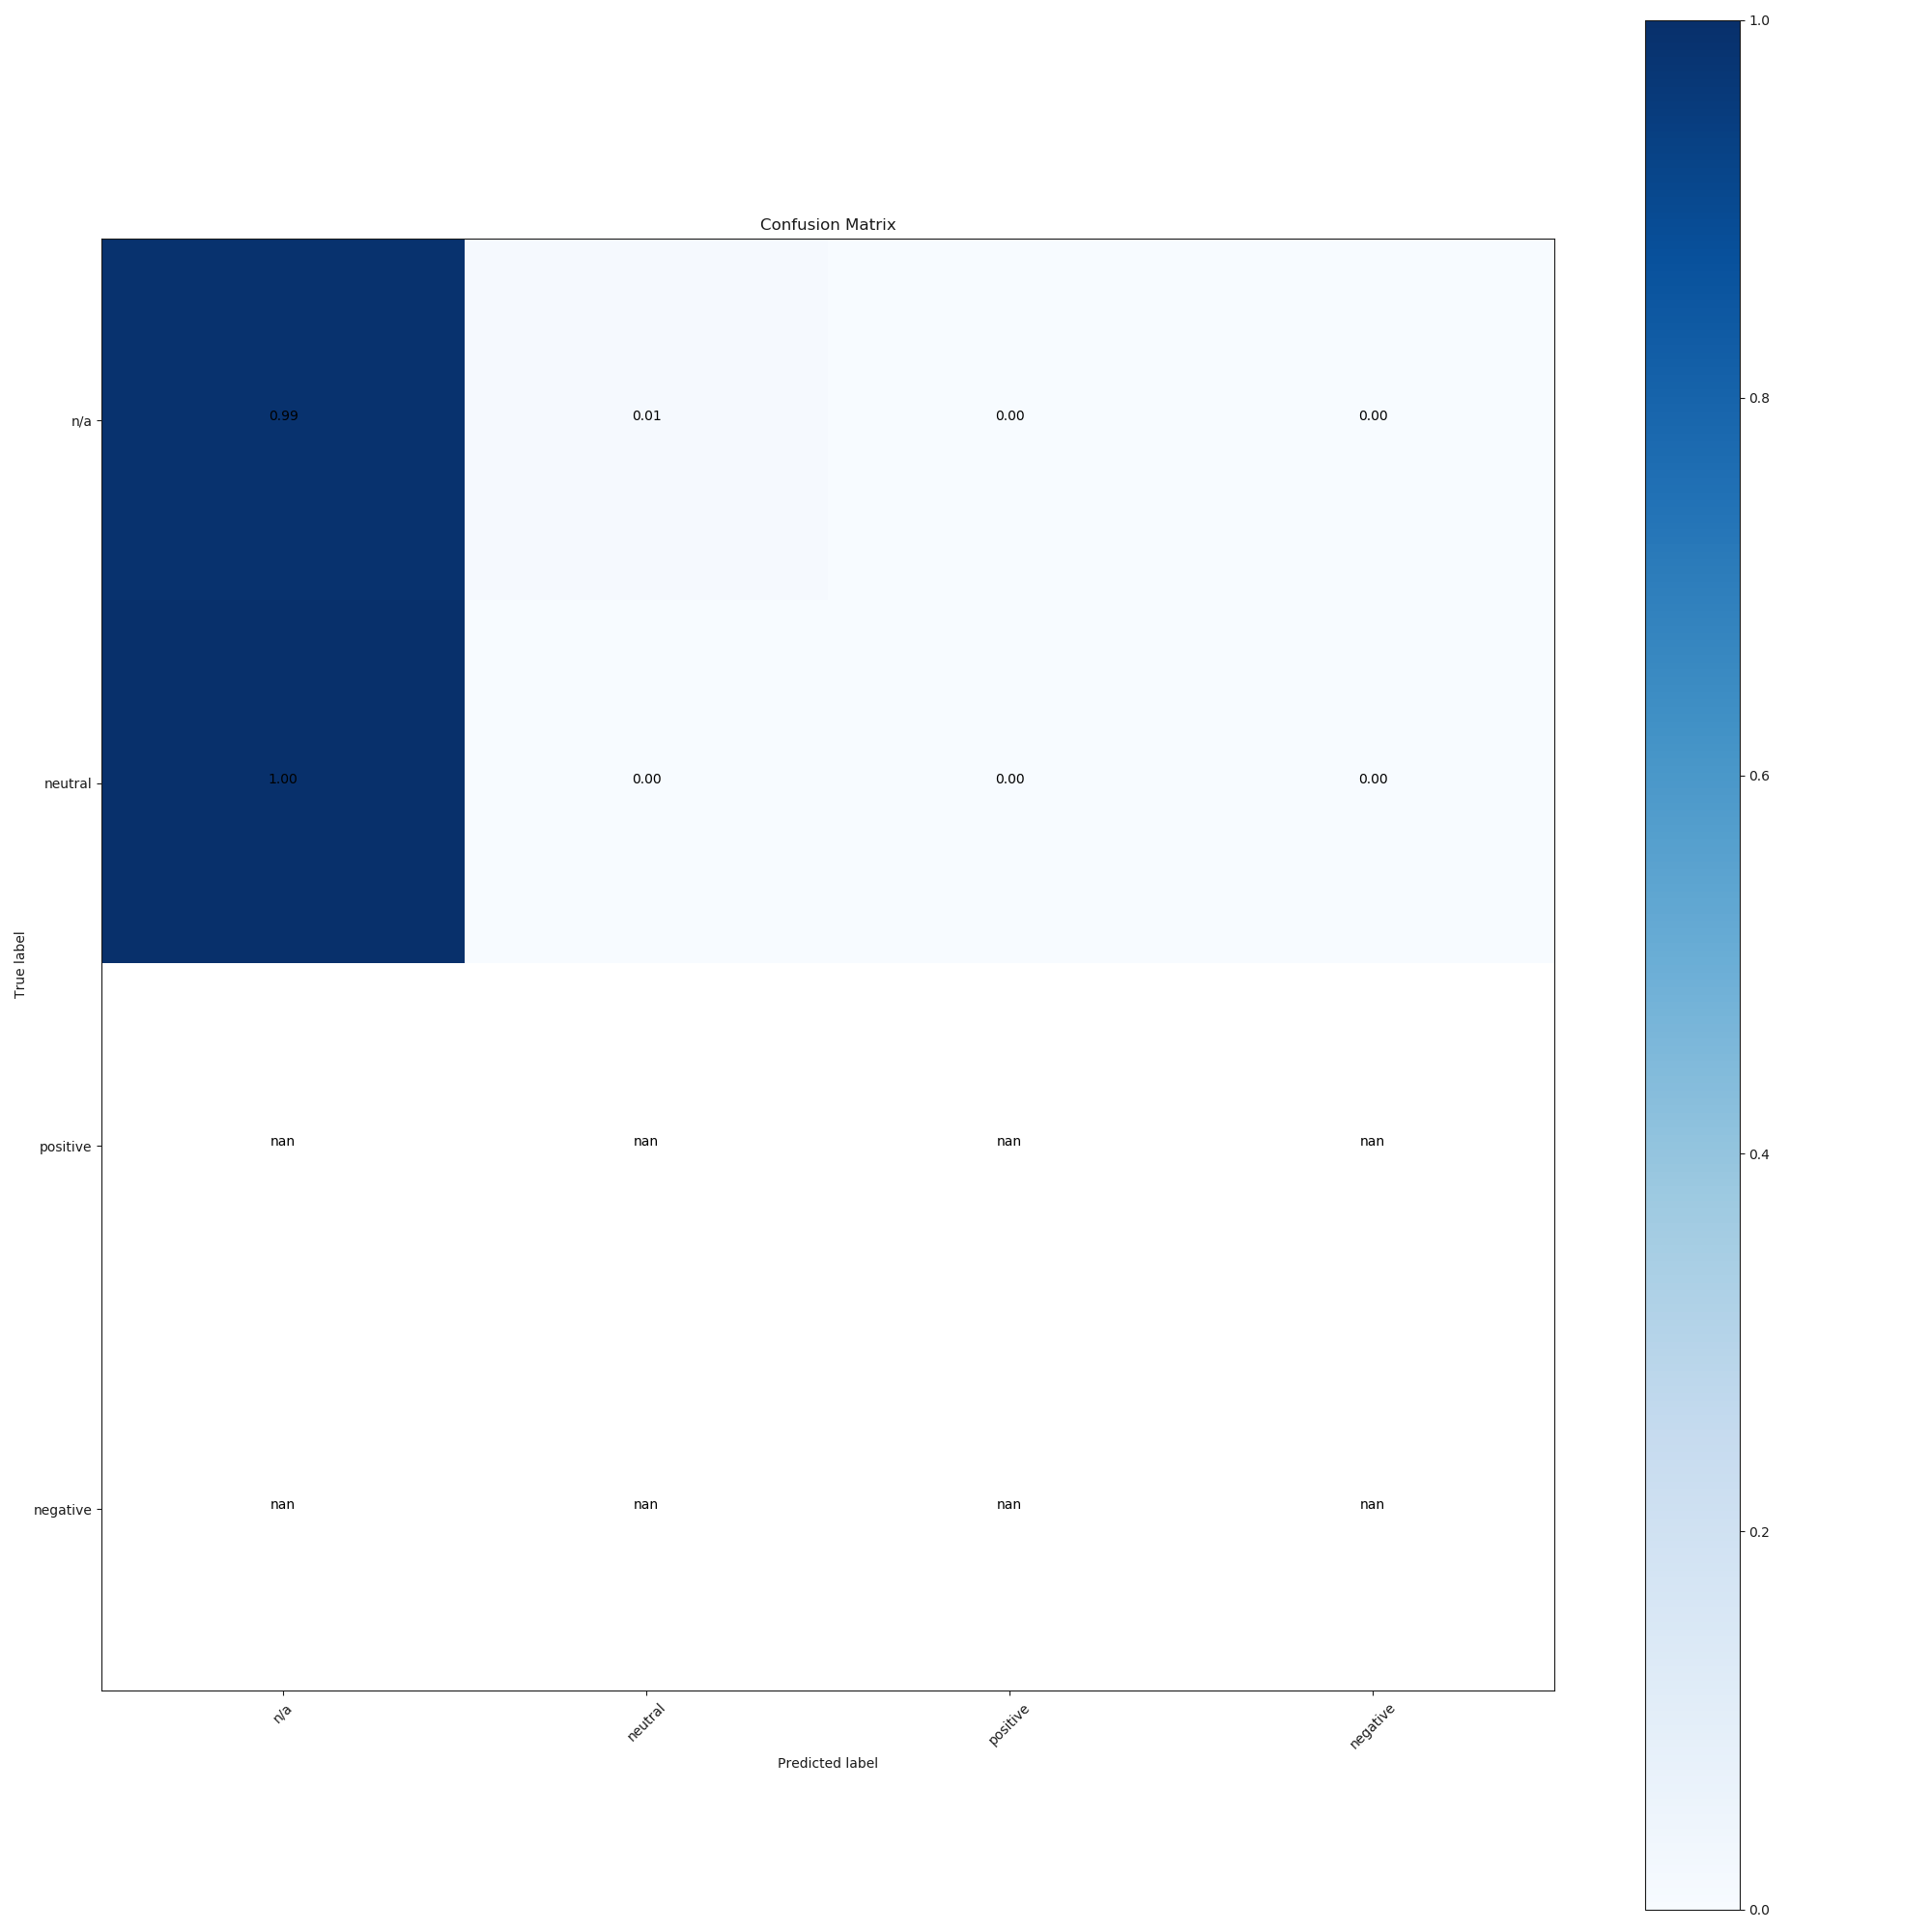
\includegraphics[width=0.19\textwidth]{figures/08_appendix/organic/08_12}
    }
    \subfloat[Organic:Environment]{
        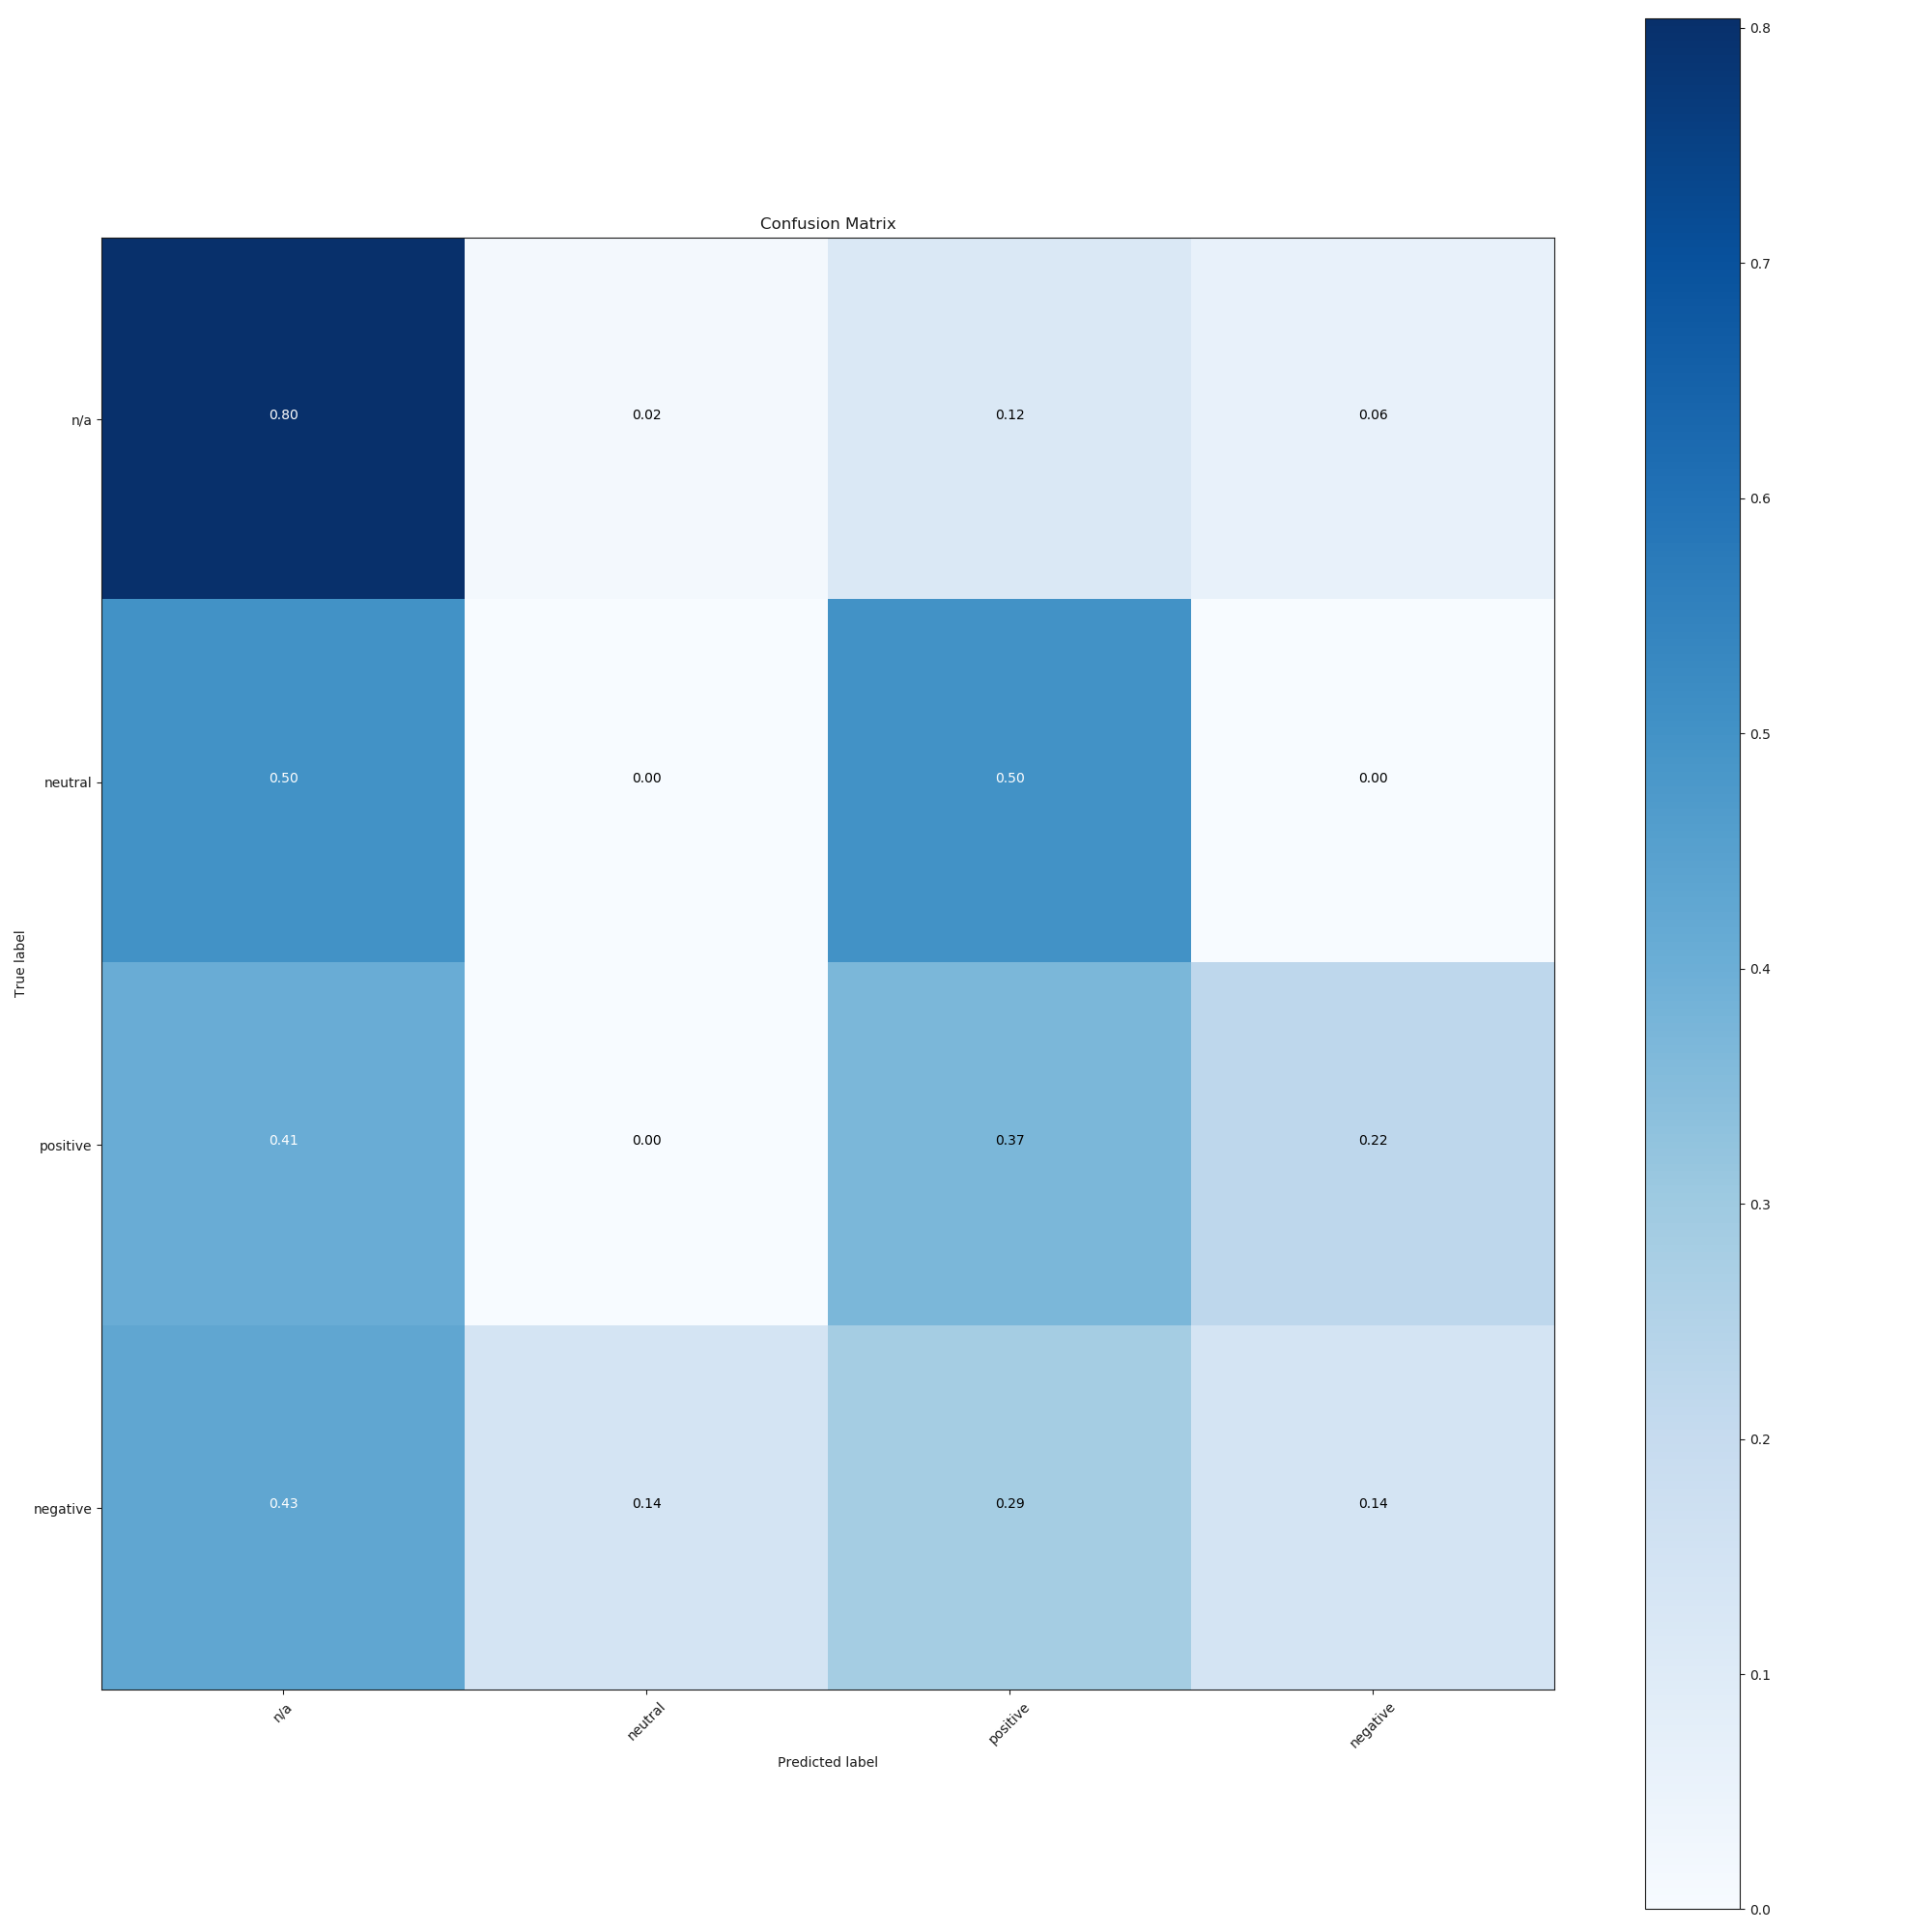
\includegraphics[width=0.19\textwidth]{figures/08_appendix/organic/08_13}
    }
    \subfloat[Organic:Quality]{
        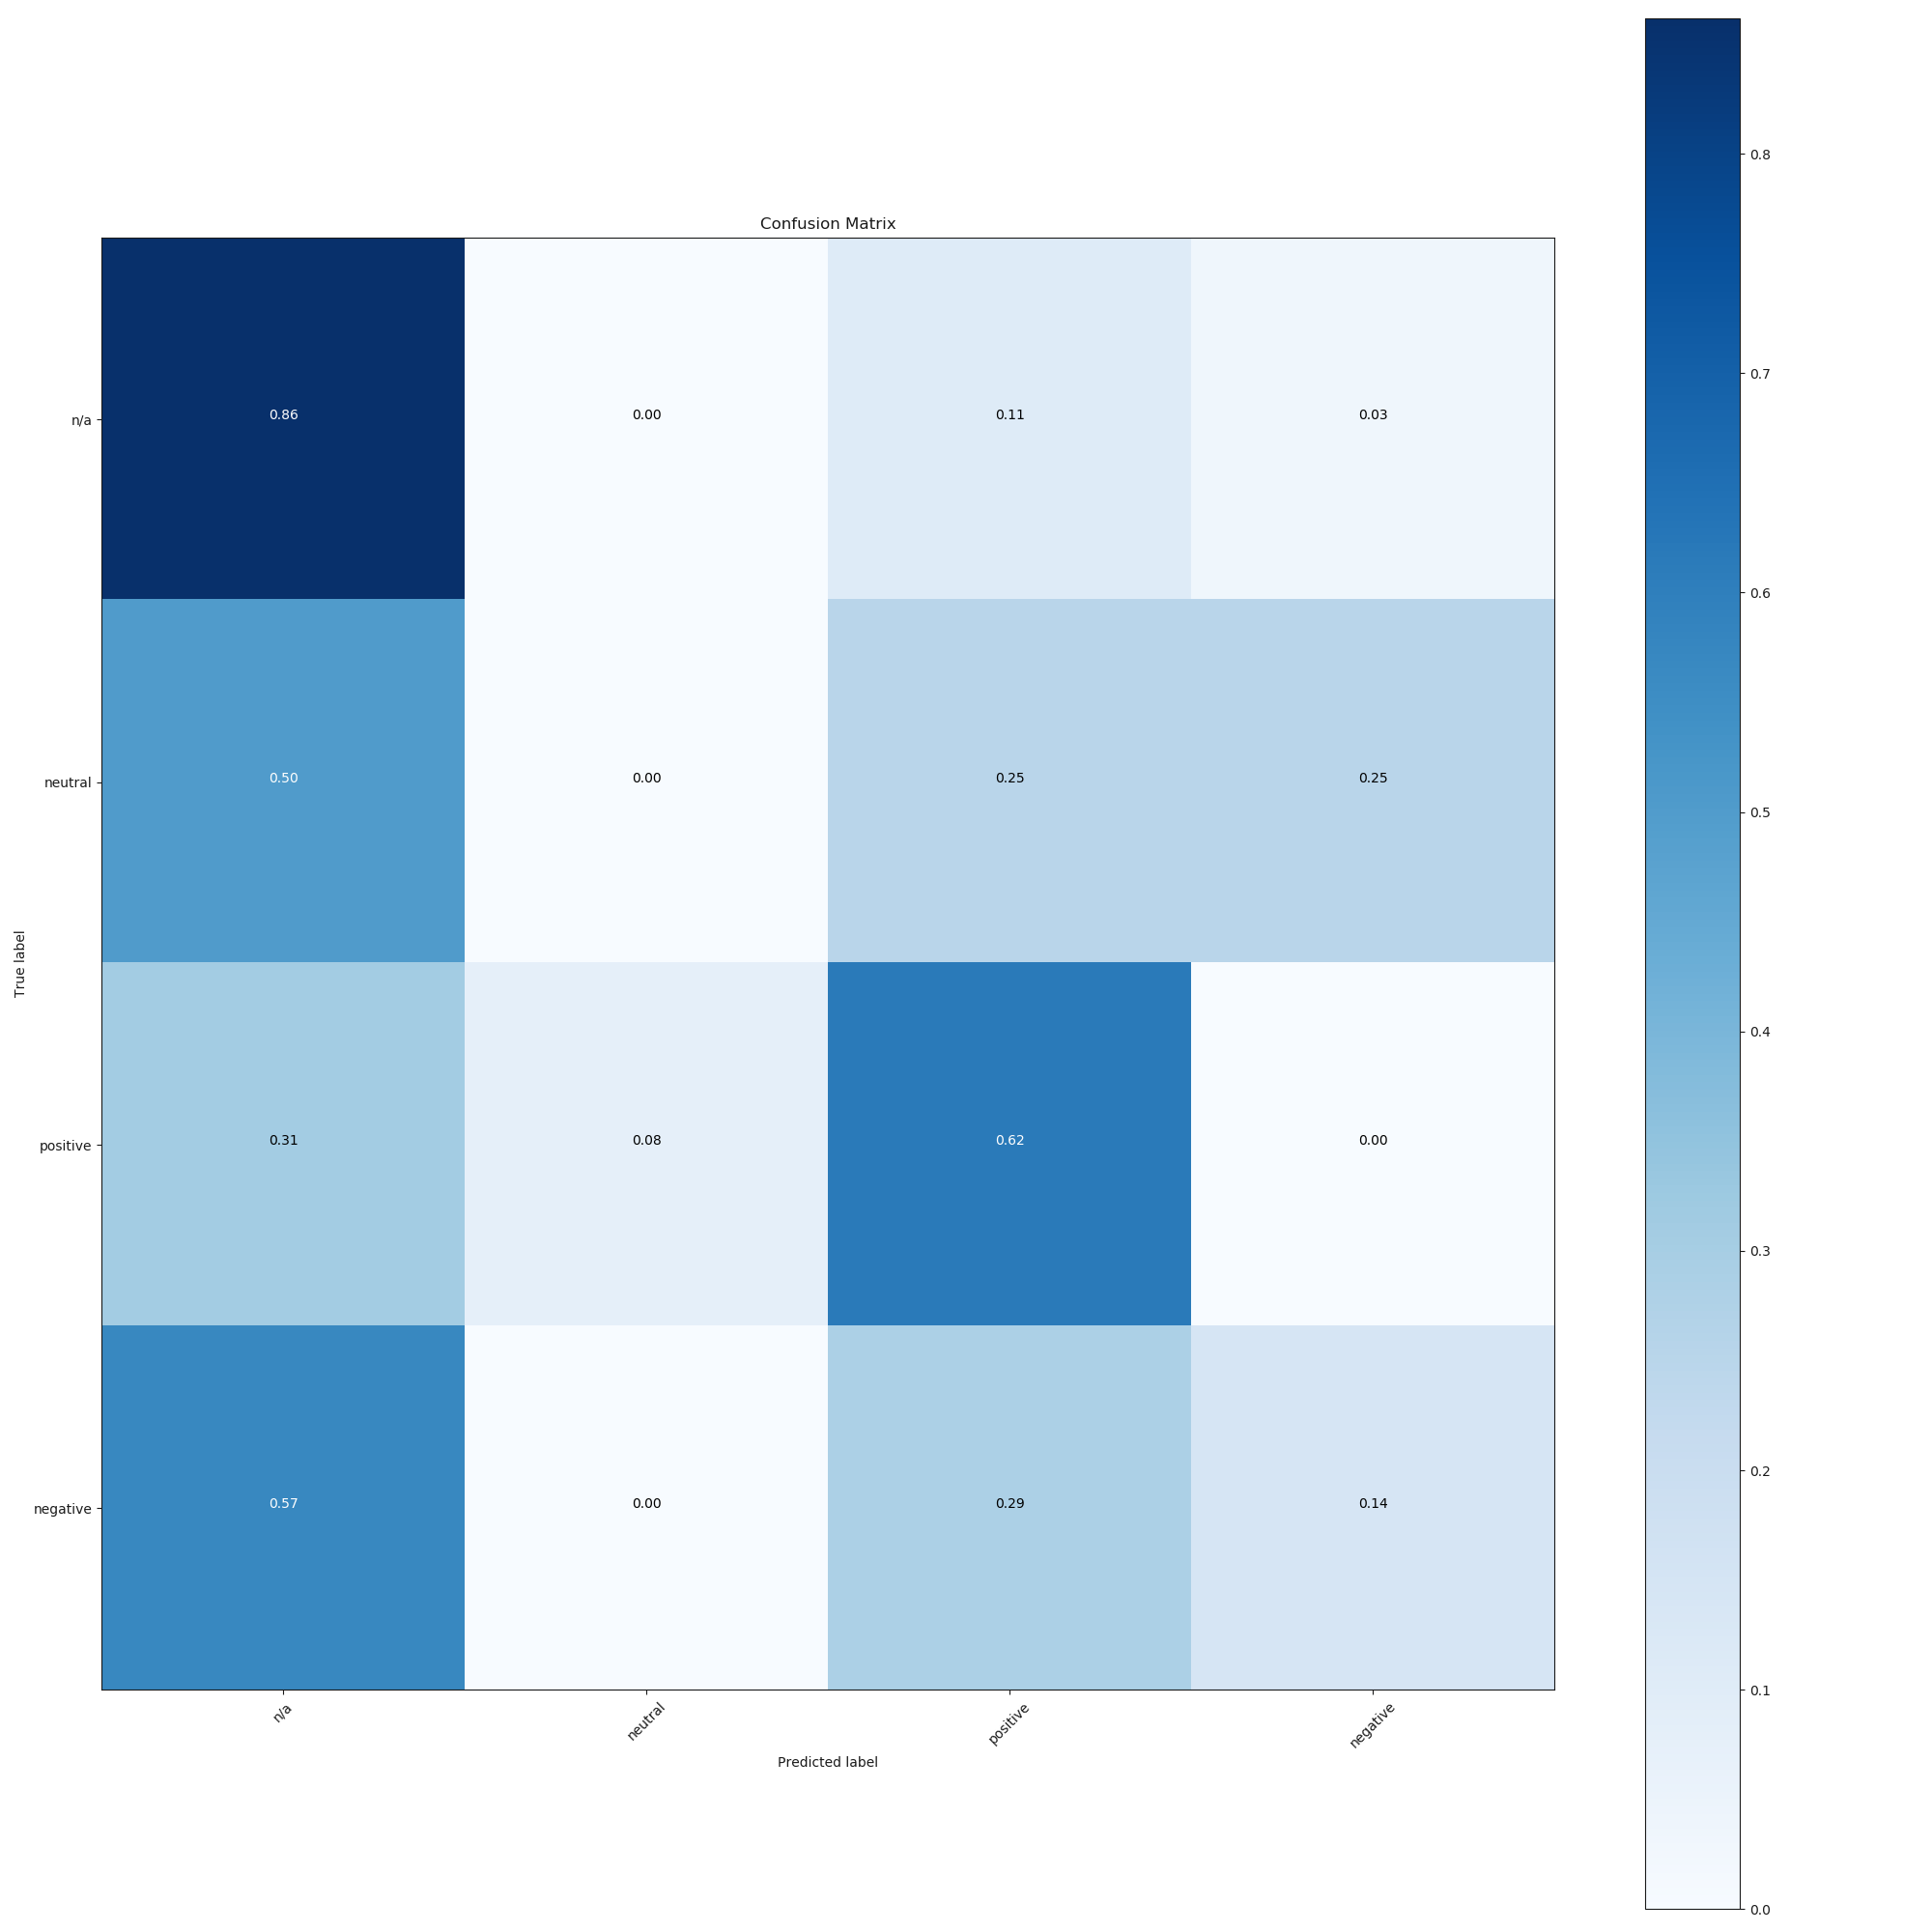
\includegraphics[width=0.19\textwidth]{figures/08_appendix/organic/08_14}
    }
    \hspace{0mm}

    \subfloat[Organic:General]{
        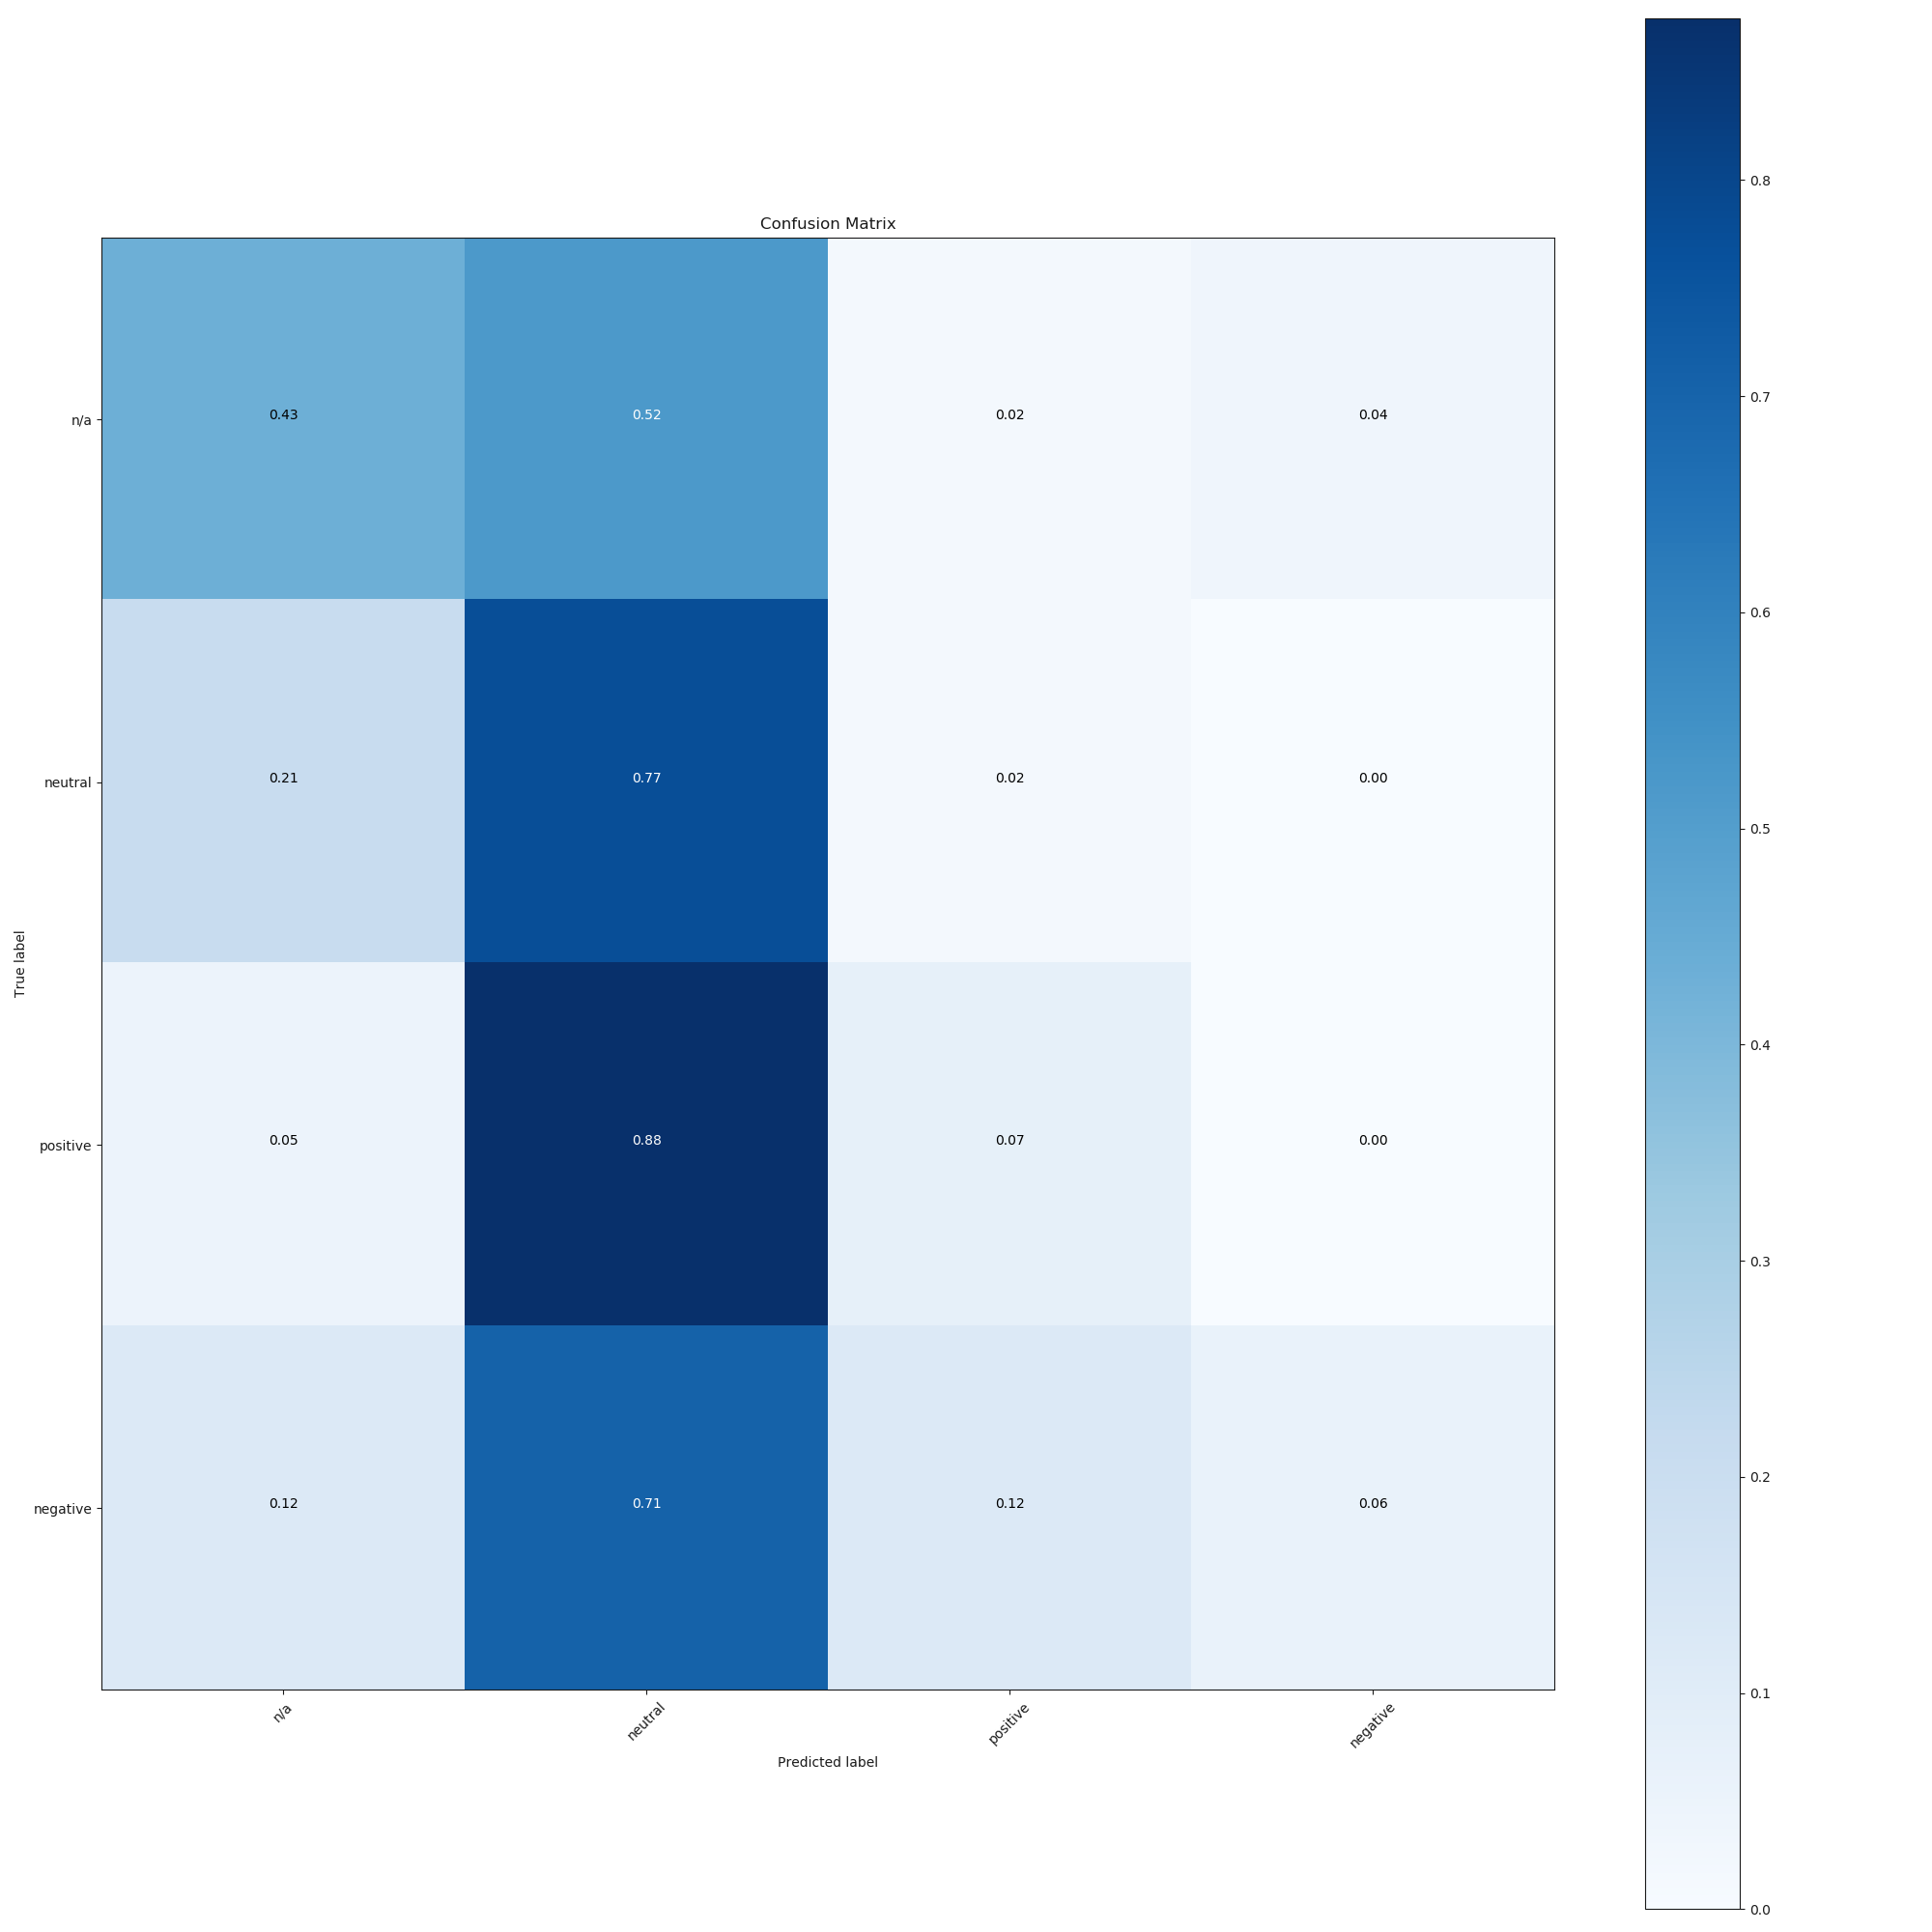
\includegraphics[width=0.19\textwidth]{figures/08_appendix/organic/08_15}
    }
    \subfloat[Organic:Price]{
        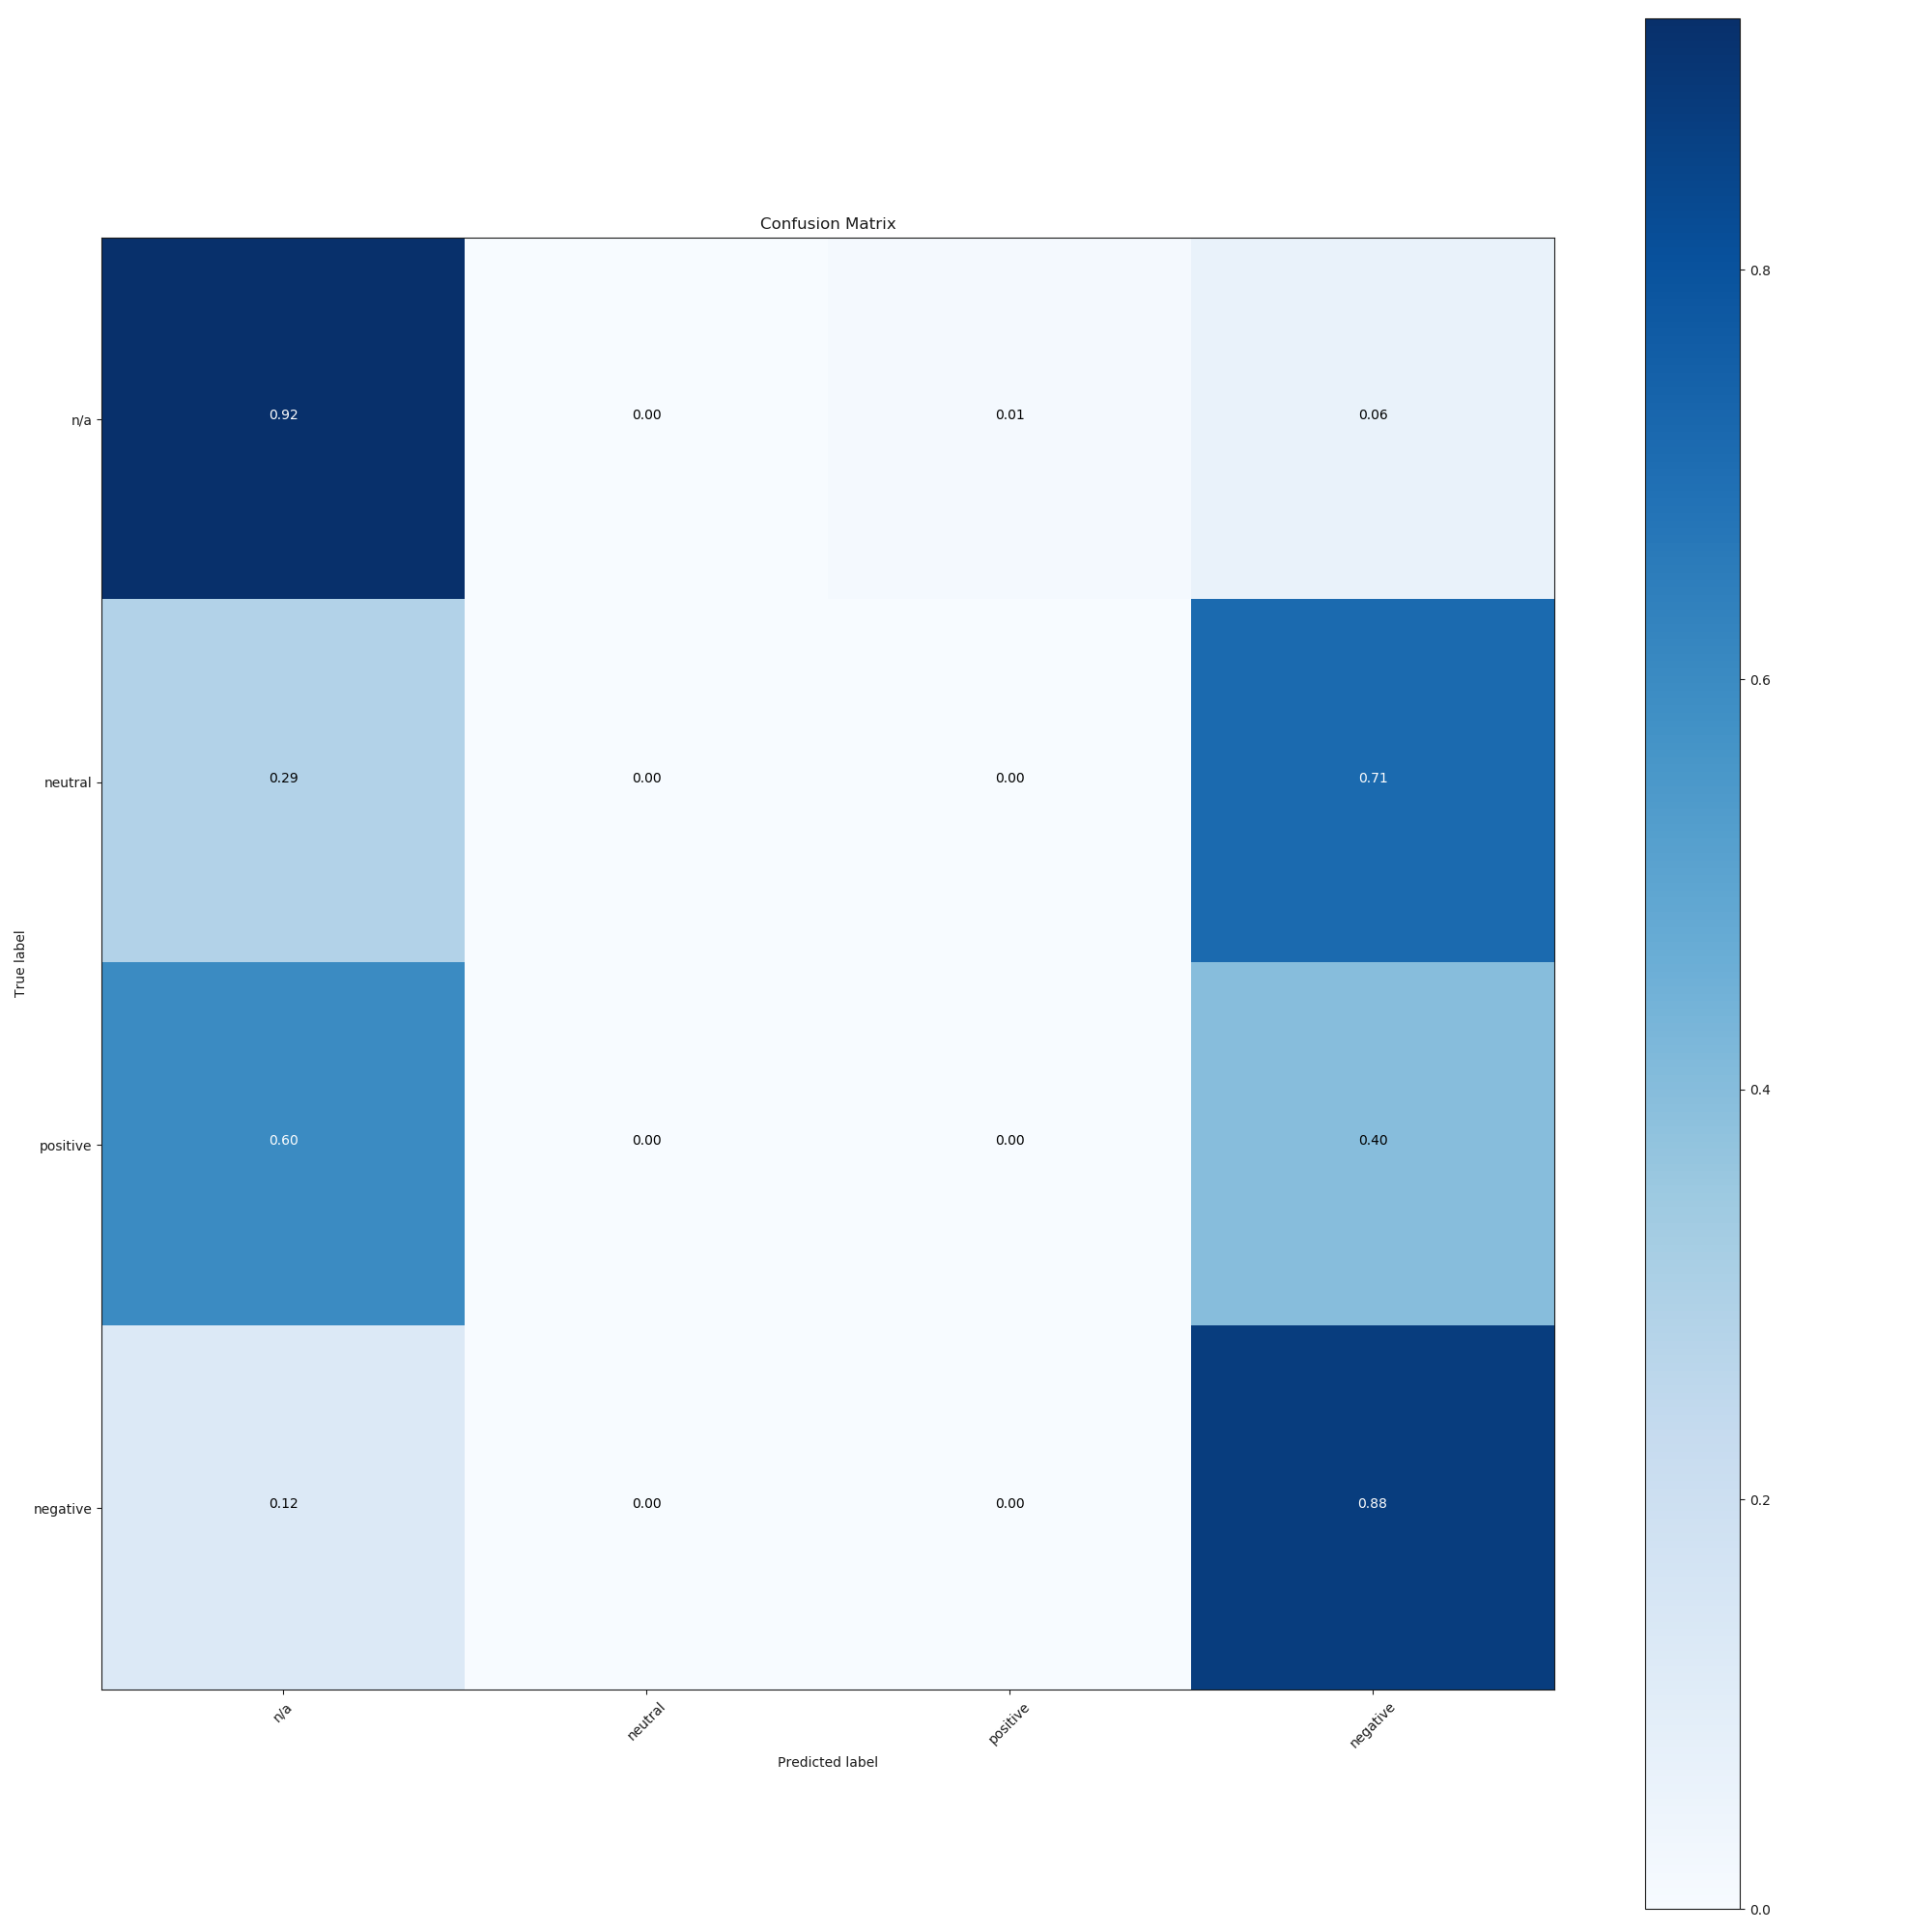
\includegraphics[width=0.19\textwidth]{figures/08_appendix/organic/08_16}
    }
    \subfloat[Organic:Safety]{
        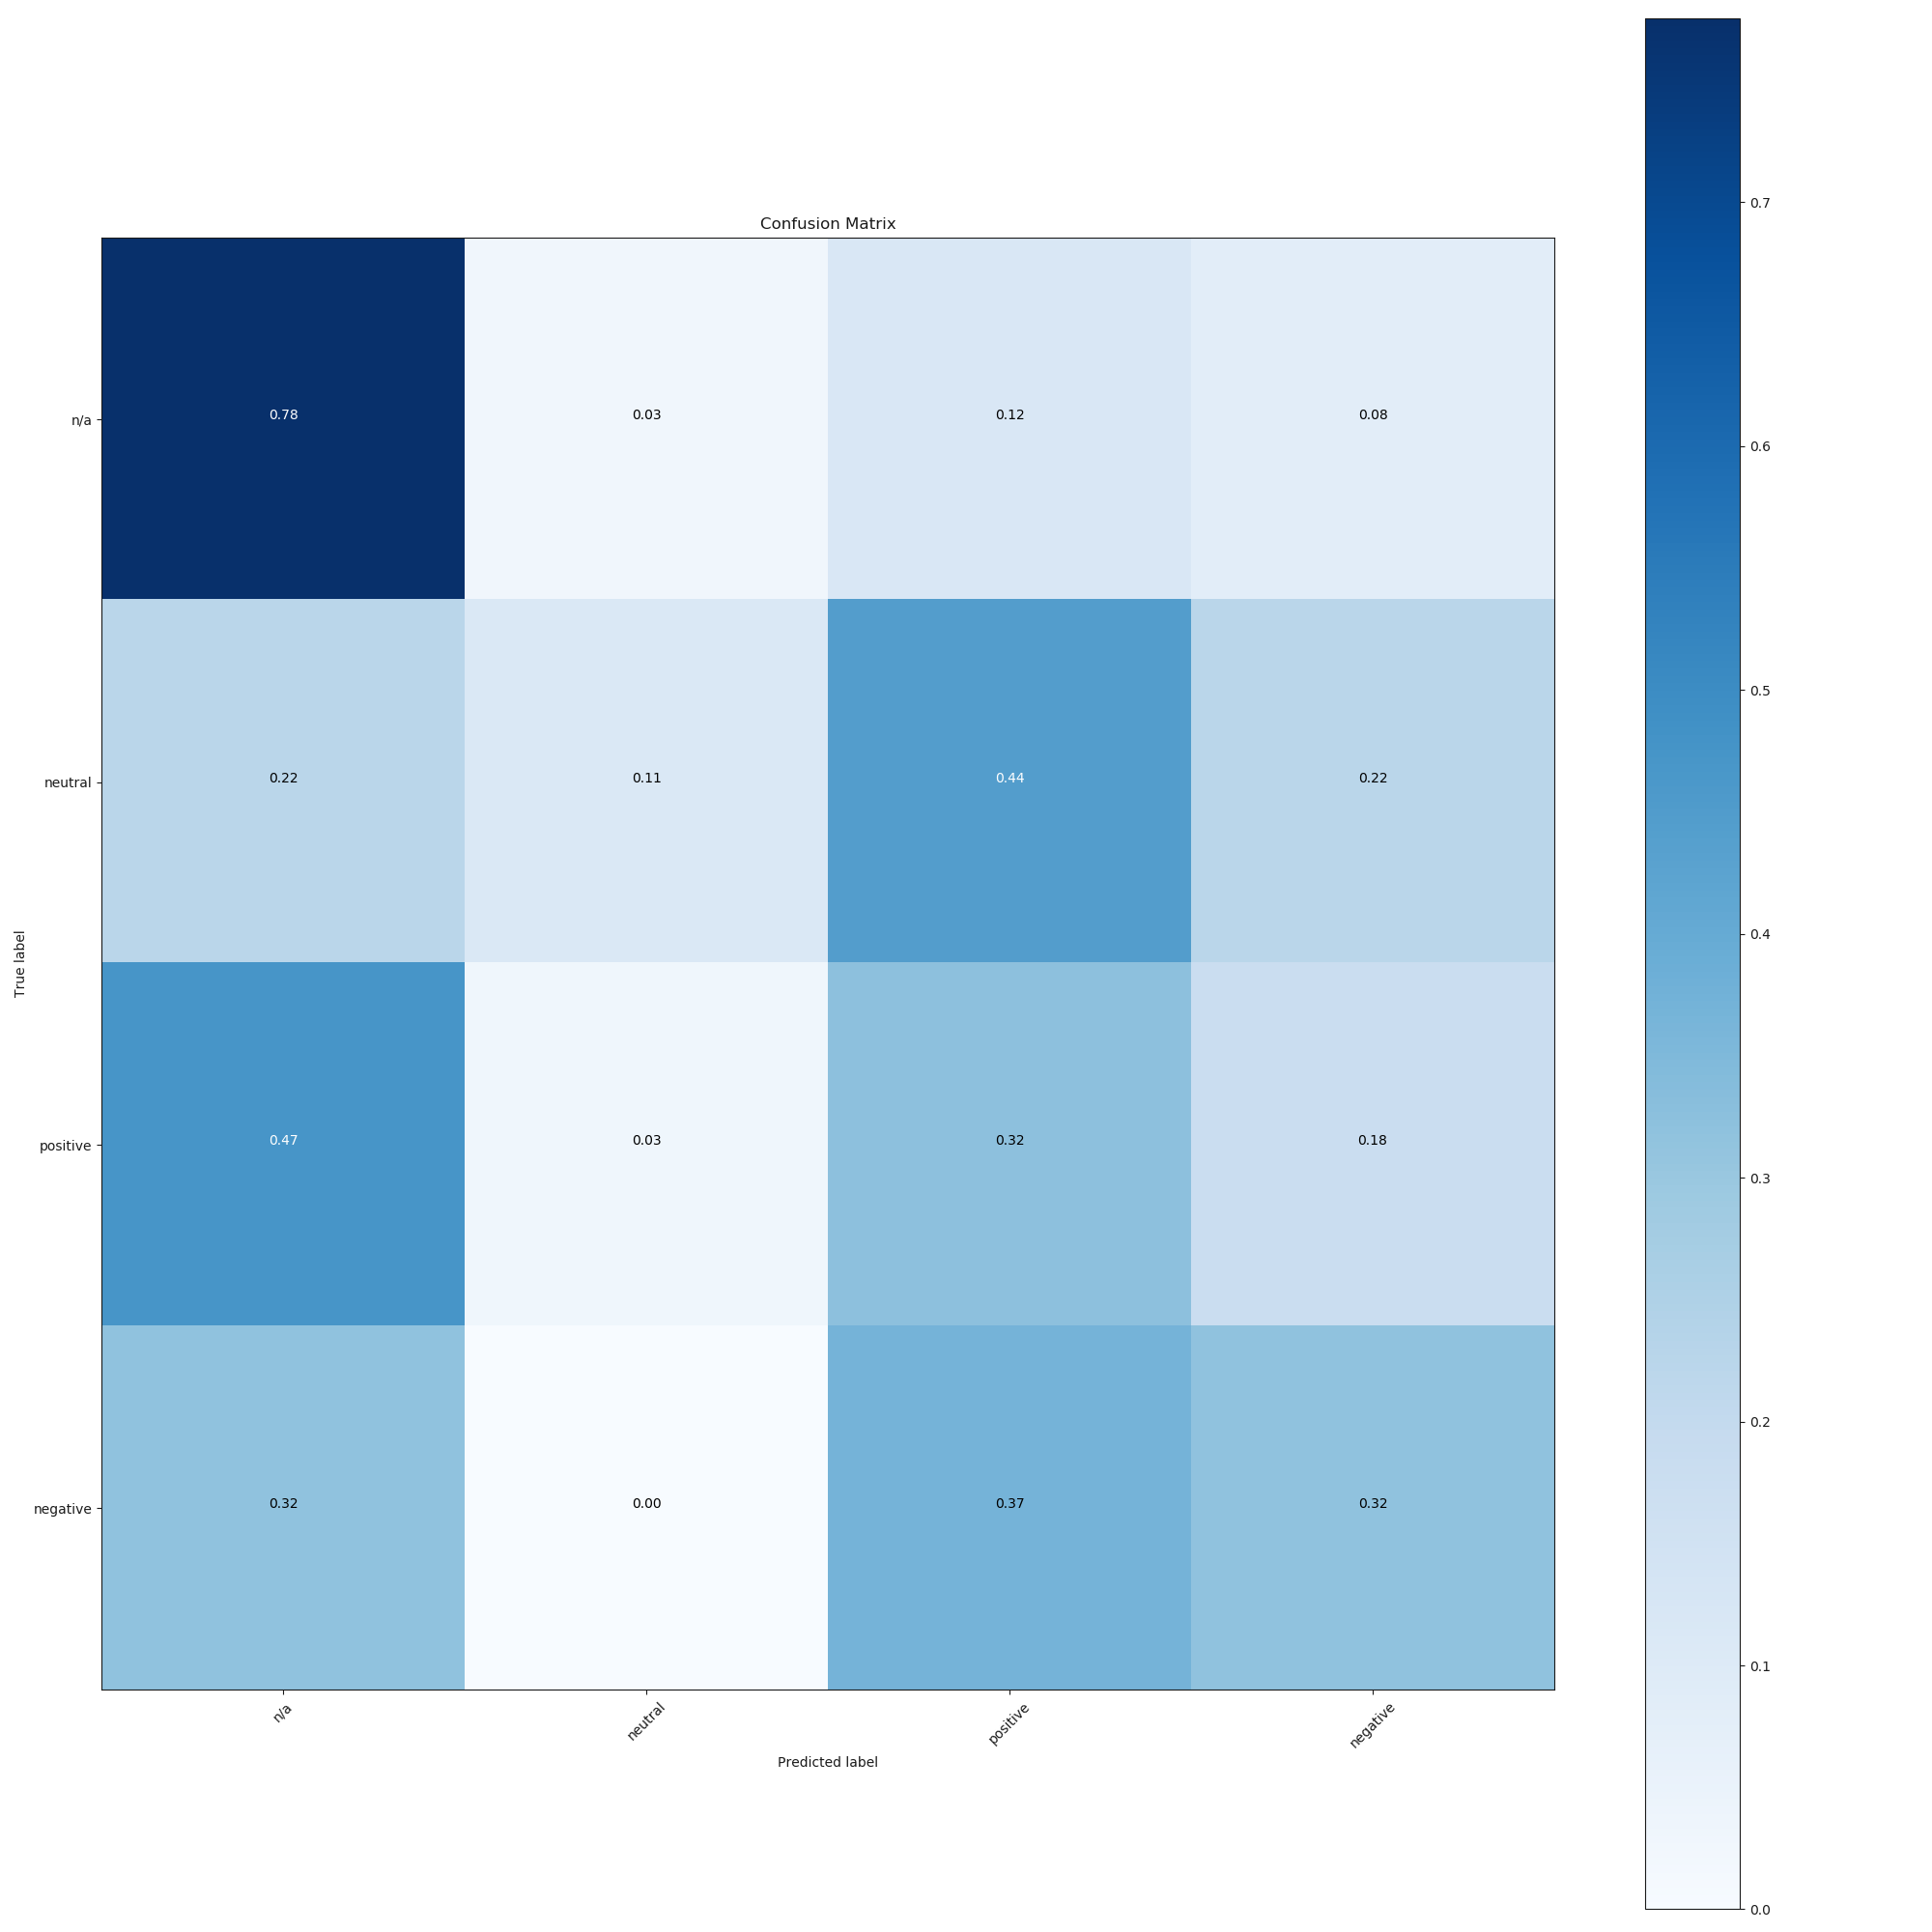
\includegraphics[width=0.19\textwidth]{figures/08_appendix/organic/08_17}
    }
    \subfloat[Organic:Sources]{
        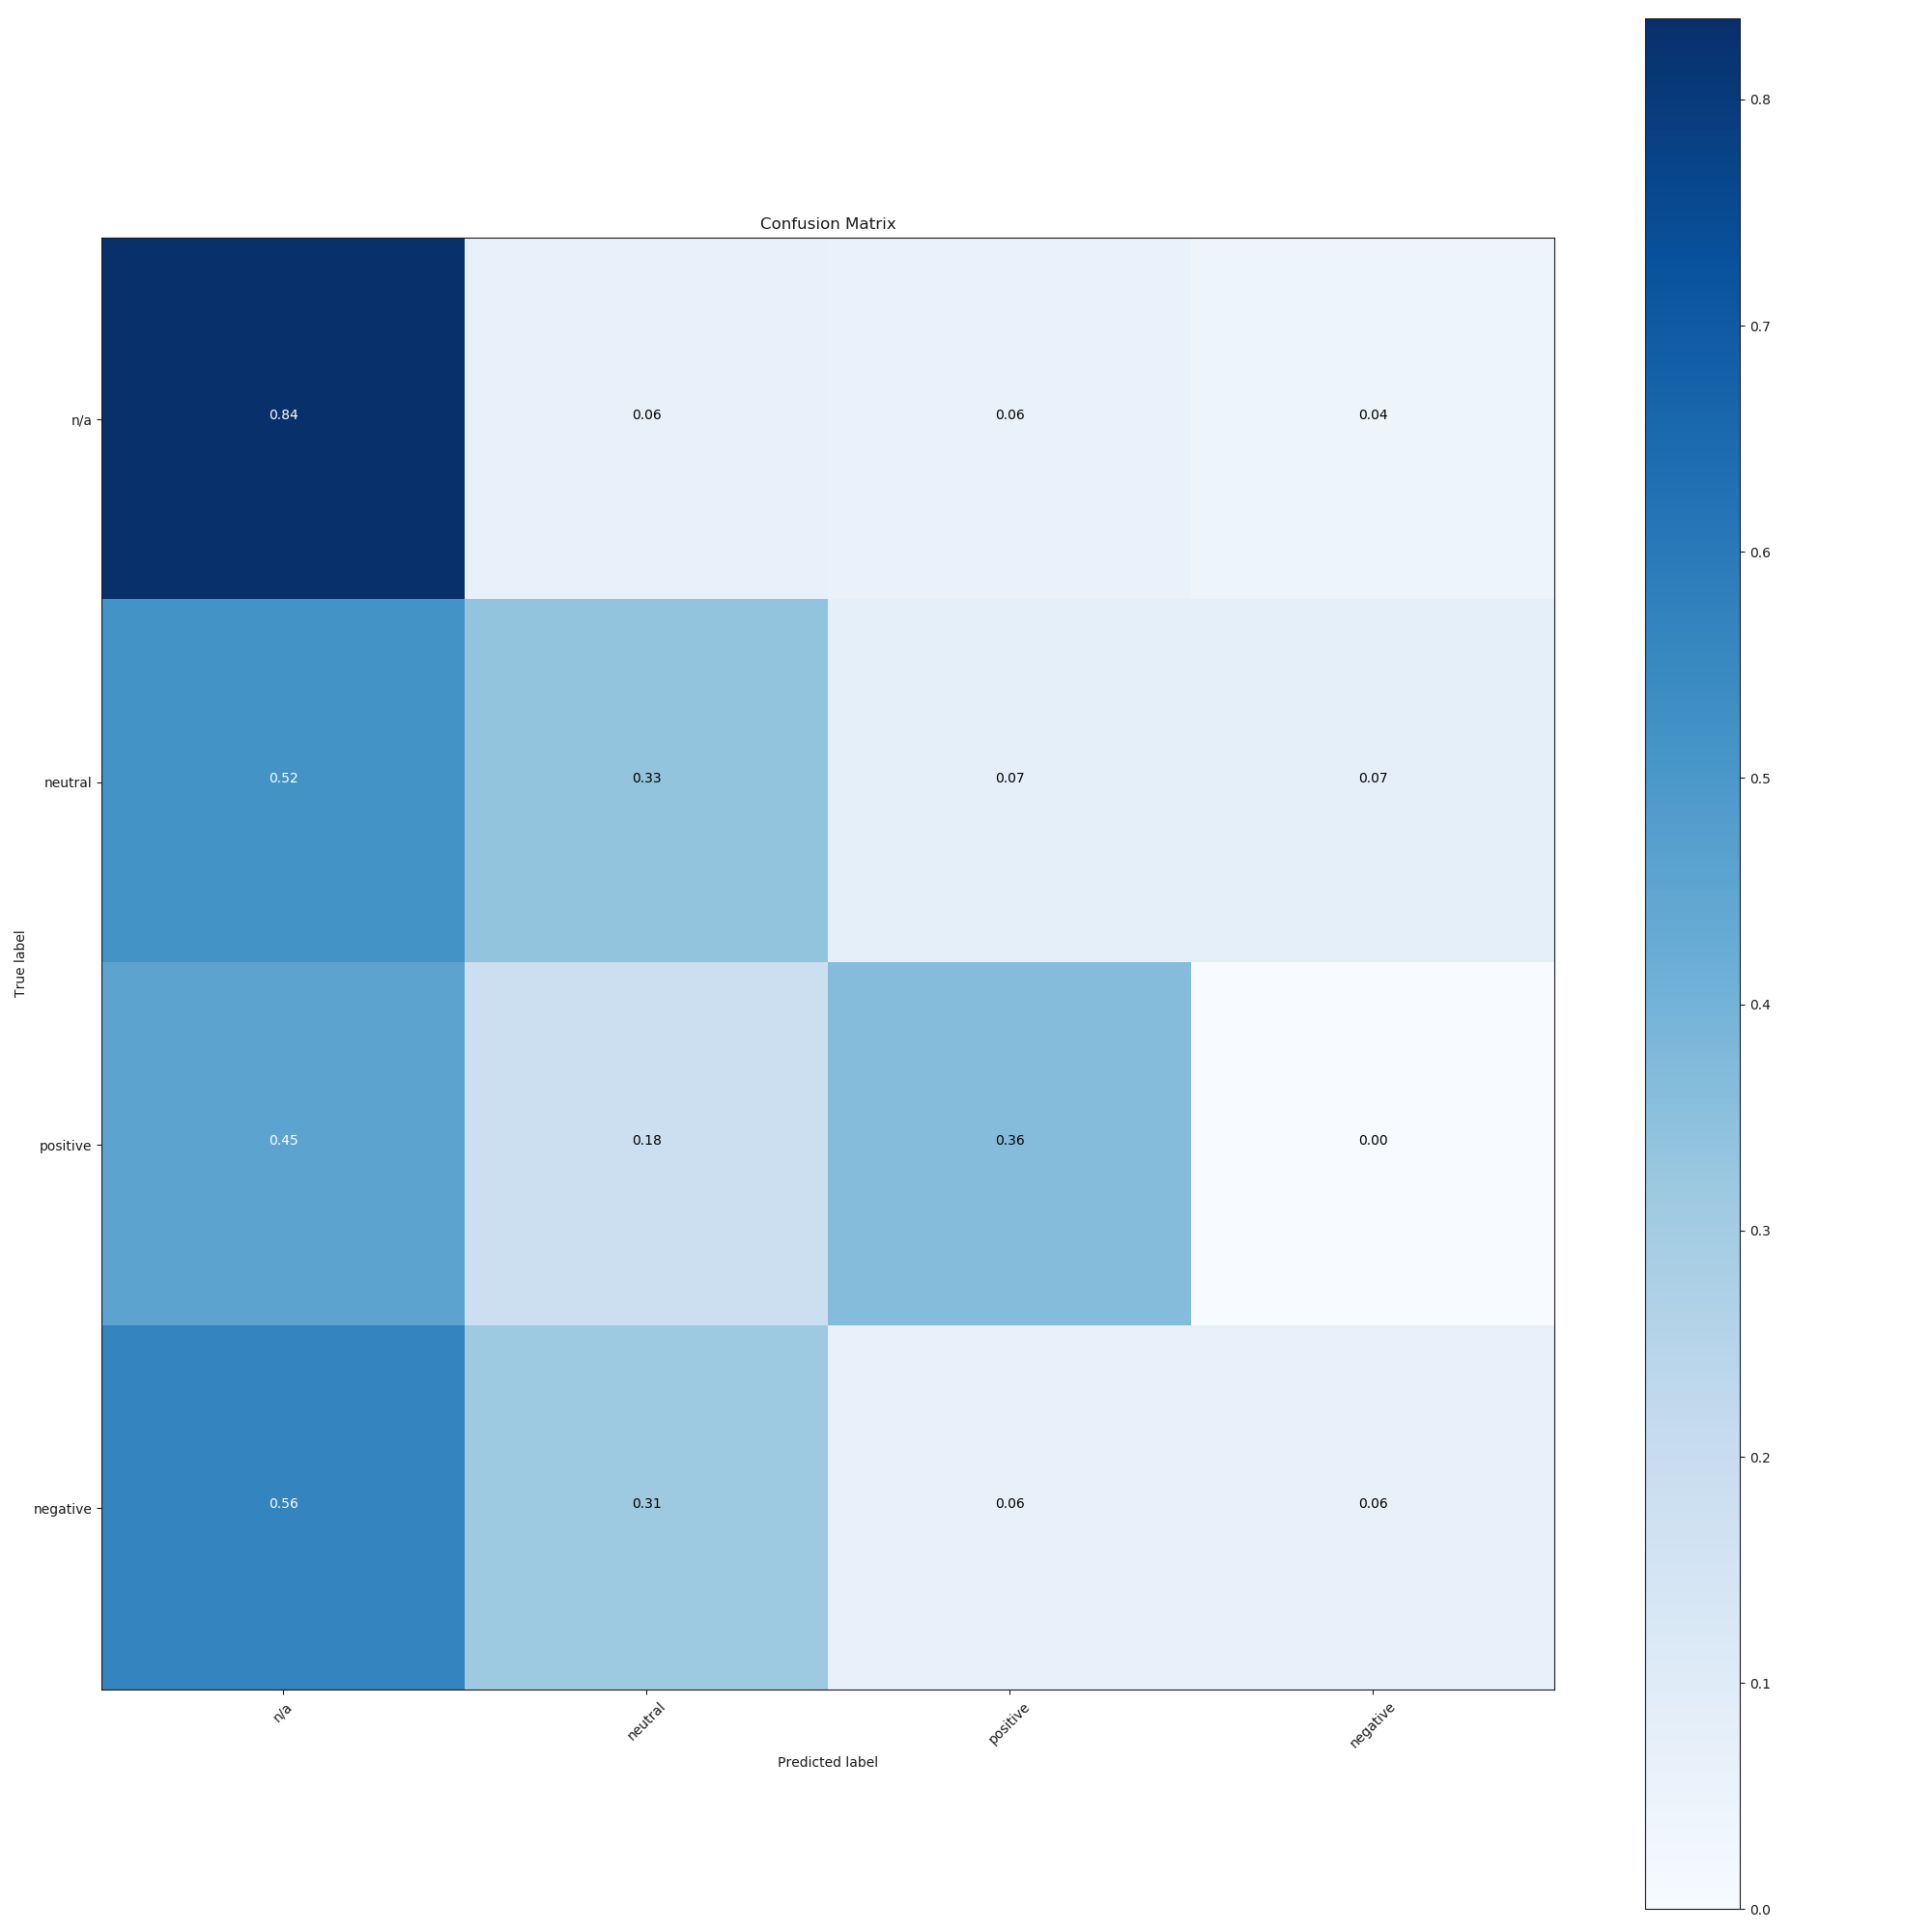
\includegraphics[width=0.19\textwidth]{figures/08_appendix/organic/08_18}
    }
	\hspace{0mm}
    \caption{\textbf{Organic-2019 Coarse Partition -- Confusion matrices of the aspect on the test split.} The figure shows a normalized confusion matrix for each aspect head. From left to right: n/a, neutral, positive, negative.}
	\label{fig:08_og_conf}

\end{figure}

\begin{figure}[H]
    \centering
    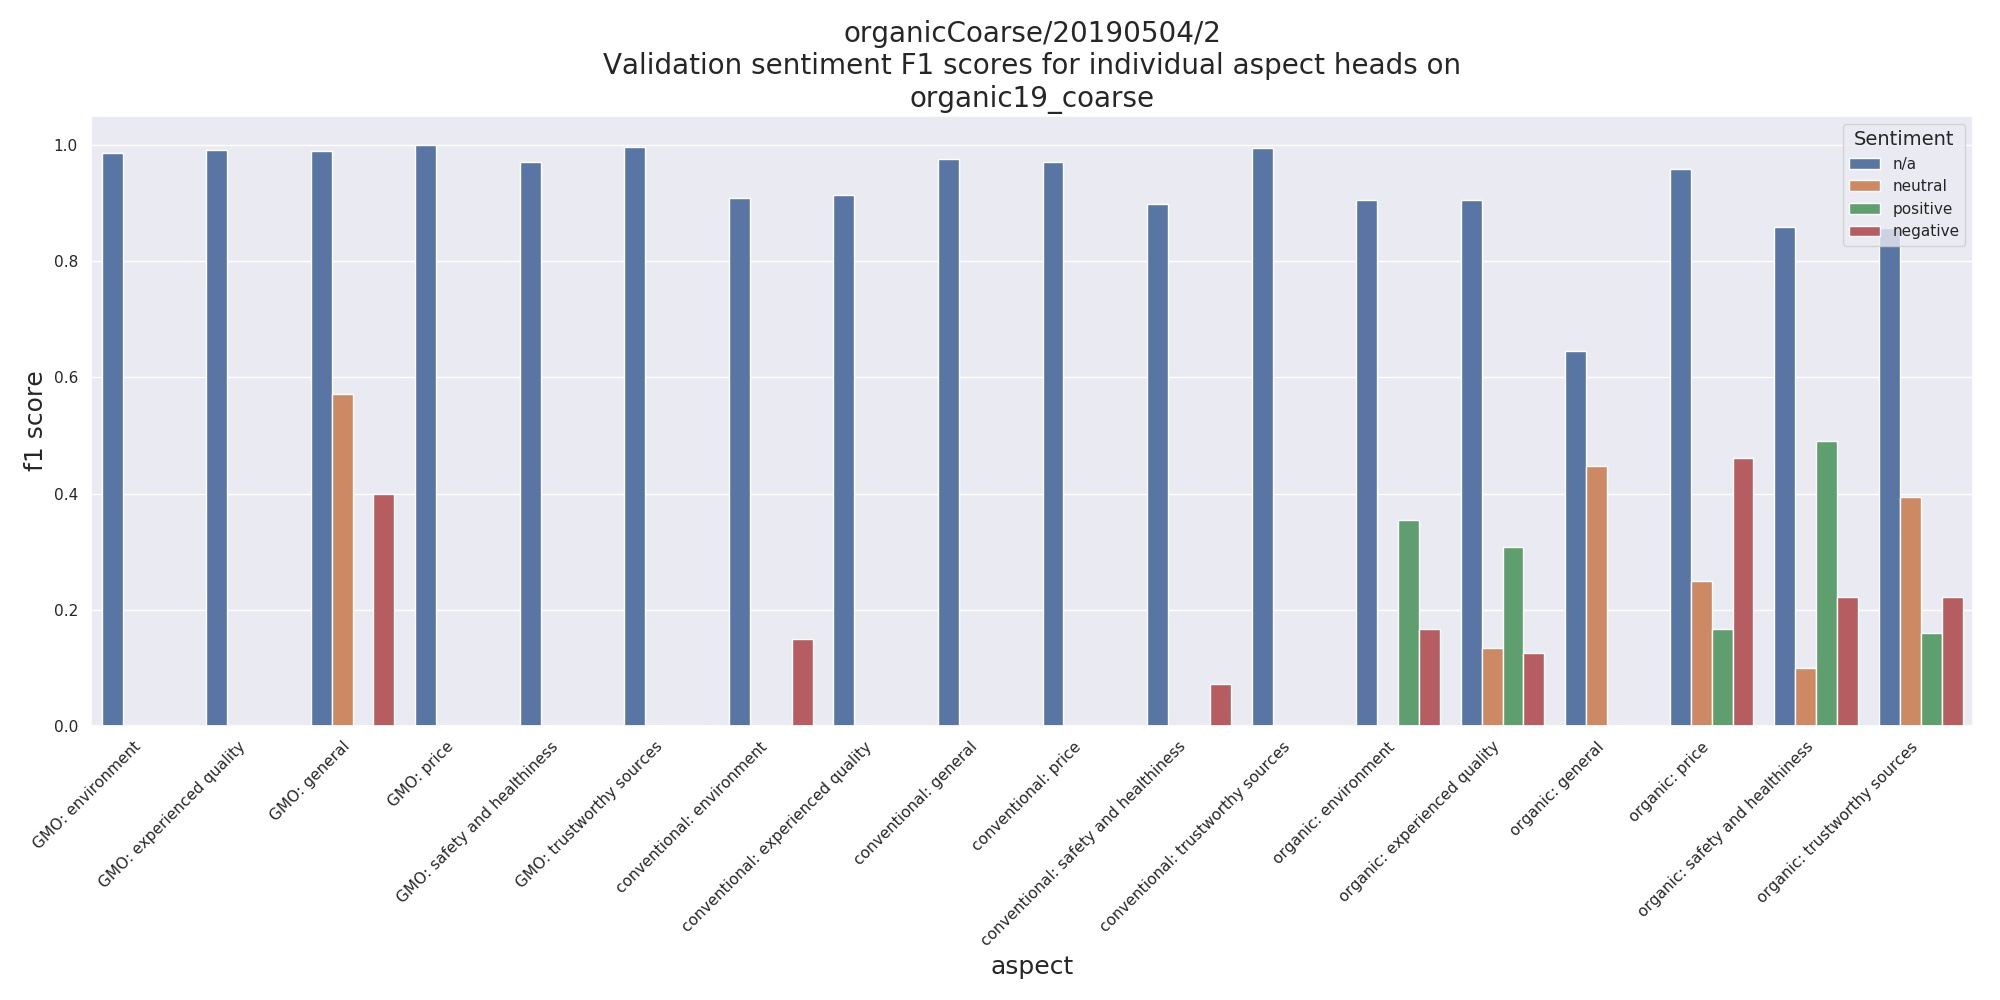
\includegraphics[width=\textwidth]{figures/08_appendix/08_og_coarse_results}
    \caption{\textbf{Organic-2019 Coarse Partition -- Micro F1 scores.} The graph visualizes the F1 scores for the sentiment class per individual aspect head. This graph demonstrates that the model does not classify classes with infrequent labels.}
    \label{fig:06_HpOptim_CnnParams2}
\end{figure}
